
%(BEGIN_QUESTION)
% Copyright 2006, Tony R. Kuphaldt, released under the Creative Commons Attribution License (v 1.0)
% This means you may do almost anything with this work of mine, so long as you give me proper credit

%Suppose you were giving instructions to a human operator regarding which way to move a hand-operated control valve to maintain a process variable at setpoint.  In each of these examples, determine which way the operator should move the valve to {\it counteract} an increase in the process variable resulting from some independent change in the process:

Du skal gi instruksjoner til en operatør no operering av håndopererte ventiler. I hvert av tilfellene nedenfor, avgjør hvilken vei han må skru. 

\vskip 30pt

\filbreak
\noindent
{\bf Example 1:} Temperaturreguleringssystem %Temperature control application

$$\includegraphics[width=15.5cm]{i00109x01.eps}$$

\vskip 30pt

\filbreak
\noindent
{\bf Example 2:} Nivåreguleringsystem %Level control application

$$\includegraphics[width=15.5cm]{i00109x02.eps}$$

\vskip 30pt

\filbreak
\noindent
{\bf Example 3:} Strømningreguleringssystem %Flow control application

$$\includegraphics[width=15.5cm]{i00109x03.eps}$$

\vskip 30pt

\filbreak
\noindent
{\bf Example 4:} Temperaturreguleringssystem %Temperature control application

$$\includegraphics[width=15.5cm]{i00109x04.eps}$$

\vskip 20pt \vbox{\hrule \hbox{\strut \vrule{} {\bf Suggestions for Socratic discussion} \vrule} \hrule}

\begin{itemize}
\item  Follow-up question: in which of these examples is the operator functioning as a {\it direct-action controller} and in which of these examples is the operator functioning as a {\it reverse-action controller}?
\end{itemize}
\medskip

\underbar{file i00109}
%(END_QUESTION)





%(BEGIN_ANSWER)

\begin{itemize}
\item  Example 1: increasing temperature, operator should close the valve more
\item  Example 2: increasing level, operator should open the valve more
\item  Example 3: increasing flow, operator should close the valve more
\item  Example 4: increasing temperature, operator should open the valve more
\end{itemize}
\medskip

The goal with these questions is to think like an operator, in order to have a clear understanding of the process's needs.  Only when one recognizes the required direction of valve operation to correct for an upset (off-setpoint) condition is it possible to properly and confidently configure an automatic controller to do the same.  This is something every instrument professional needs to consider when designing and/or commissioning a control system: {\it which way does the final control element need to go, in order to stabilize the process variable if it deviates too high?}

\vskip 10pt

In the first example, we would need to move the fuel gas valve further closed (toward the shutoff position) if ever the temperature got too high.

\vskip 10pt

In the second example, we would need to move the drain valve further open to correct for a too-high liquid level in the vessel.

\vskip 10pt

In the third example, we would need to move the flow control valve further closed (toward shutoff) if ever the flow rate measured too high.

\vskip 10pt

In the fourth example, we would need to open the control valve further in order to reduce a too-high oil temperature exiting the heat exchanger.  The rationale for this direction of valve motion is to increase the flow rate of the oil so that each molecule spends less time in the heat exchanger absorbing heat from steam and increasing in temperature.

%(END_ANSWER)





%(BEGIN_NOTES)


%INDEX% Control, basics: direct versus reverse action

%(END_NOTES)



%(BEGIN_QUESTION)
% Copyright 2006, Tony R. Kuphaldt, released under the Creative Commons Attribution License (v 1.0)
% This means you may do almost anything with this work of mine, so long as you give me proper credit

%In any automated (controlled) system, there is a {\it process variable}, a {\it setpoint}, and a {\it manipulated variable}.  There is also something called a {\it load}, which influences how well the control system is able to maintain setpoint.  Provide a general description for a ``load,'' and then identify the load(s) in each of the following manually-controlled processes:

I alle reguleringssystem er det en Prosessvariabel (PV), et settpunkt (SP) og en manipulerendevariabel (MV). Det er også noe kalt last som er med på å avgjøre hvor godt systemet holder settpunktet. Gi en generell beskrivelse av last og identifiser lastene i eksemplene nedenfor. 


\vskip 30pt

\noindent
{\bf Example 1:} Temperaturreguleringssystem % Temperature control application

$$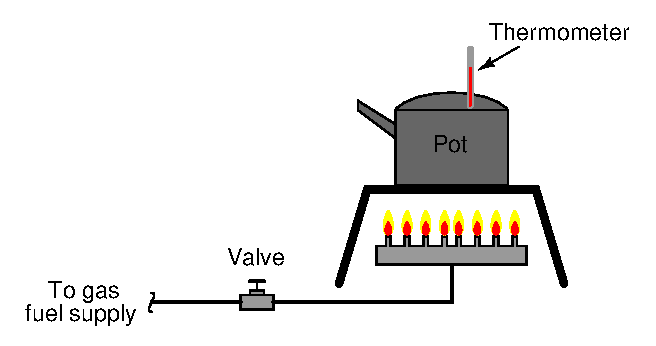
\includegraphics[width=15.5cm]{i01453x01.eps}$$

\vskip 30pt

\filbreak
\noindent
{\bf Example 2:} Nivåreguleringssystem % Level control application

$$\includegraphics[width=15.5cm]{i01453x02.eps}$$

\vskip 30pt

\filbreak
\noindent
{\bf Example 3:} Strømningsreguleringssystem % Flow control application

$$\includegraphics[width=15.5cm]{i01453x03.eps}$$

\vskip 30pt

\filbreak
\noindent
{\bf Example 4:} Temperaturreguleringssystem % Temperature control application

$$\includegraphics[width=15.5cm]{i01453x04.eps}$$

\vskip 20pt \vbox{\hrule \hbox{\strut \vrule{} {\bf Suggestions for Socratic discussion} \vrule} \hrule}

\begin{itemize}
\item  Explain why ambient air temperature is considered a {\it load} to process example \#4, but the insulation thickness on the heat exchanger is not.
\end{itemize}
\medskip

\underbar{file i01453}
%(END_QUESTION)





%(BEGIN_ANSWER)

A {\it load} is any variable in a process (besides the manipulated variable) that has influence over the process variable being controlled.

\vskip 10pt

Note: the following answers are not exhaustive.  In other words, there may be more loads than what is listed here for each process!

\begin{itemize}
\item  Example 1: ambient air temperature
\item  Example 2: incoming flow rate
\item  Example 3: upstream and downstream pressures
\item  Example 4: steam flow rate, steam temperature
\end{itemize}
\medskip

%(END_ANSWER)





%(BEGIN_NOTES)

Students may be tempted to list process {\it constants} (such as vessel volume, heat exchanger tube thickness, etc.) as loads because they do impact the process dynamics.  However, the term ``load'' is typically reserved for some {\it variable} that has impact over the process, and is thus liable to change over time in such a way to challenge the loop controller.

To put this in different terms, the need to change setpoints, and the existence of variable loads in a process, both {\it justify} the presence of a controller.  If we were faced with a process never needing a different setpoint, and devoid of variable loads, there would be no need to place a control loop in it!  We could simply set a manually-actuated control valve where we wanted it to be, and leave it in that position forever!

\vfil \eject

\noindent
{\bf Prep Quiz:}

The definition of a {\it load} with regard to process control loops is:

\begin{itemize}
\item  The time lag between a change in output and a change seen in the PV
\vskip 5pt 
\item  The value at which the control system attempts to stabilize the PV over time
\vskip 5pt 
\item  A device that dissipates energy in a circuit, as opposed to sourcing energy to the circuit
\vskip 5pt 
\item  The multiplication factor of a process, measured from output to input
\vskip 5pt 
\item  A drain of energy on a system, causing it to operate inefficiently
\vskip 5pt 
\item  A variable affecting the PV, that is itself unregulated by the control system
\end{itemize}
\medskip



%INDEX% Control, basics: load (definition)

%(END_NOTES)



%(BEGIN_QUESTION)
% Copyright 2006, Tony R. Kuphaldt, released under the Creative Commons Attribution License (v 1.0)
% This means you may do almost anything with this work of mine, so long as you give me proper credit

Definer følgende begreper med tanke på P-regulatorer:

\begin{itemize}
\item{} Proporsjonalbånd
\item{} Forsterkning (Gain)
\end{itemize}

Hvilket av disse to begrepene forteller oss hvor mye regulatoren reagerer på endringer i avviket? Forklar ditt svar med et eksempel.

\vfil

\underbar{file i01461}
\eject
%(END_QUESTION)





%(BEGIN_ANSWER)

{\it Proporsjonalbånd} er definert som mengden av endring i prosessvariabelen som er nødvendig for å endre regulatorens utgang (pådrag) fra 0\% til 100\%.

{\it Forsterkning} er definert som forholdet mellom endring i utgang og endring i inngang.

$$\mbox{Forsterkning} = \frac{\Delta \mbox{Utgang}}{\Delta \mbox{Inngang}}$$

Begge begrepene kvantifiserer responsiviteten til en regulator.

%(END_ANSWER)





%(BEGIN_NOTES)

Det er viktig at studentene forstår at {\it proporsjonalbånd} og {\it forsterkning} (gain) er to forskjellige måter å uttrykke nøyaktig det samme på: hvor kraftig regulatoren vil reagere på endringer i inngangssignalet (avviket). Sørg for at du diskuterer inversiteten mellom de to: en regulator med høy forsterkning har et smalt proporsjonalbånd, og omvendt.

%INDEX% Control, proportional: proportional band versus gain

%(END_NOTES)

%(BEGIN_QUESTION)
% Copyright 2006, Tony R. Kuphaldt, released under the Creative Commons Attribution License (v 1.0)
% This means you may do almost anything with this work of mine, so long as you give me proper credit

%Convert the following controller gain settings into units of proportional band:

Konverter følgende regulatorinstillinger for forsterkning om til proporsjonalbånd. 

\medskip 
\begin{itemize}
\item Gain = 1; P.B. = \underbar{\hskip 50pt}
\vskip 5pt
\item Gain = 2; P.B. = \underbar{\hskip 50pt} 
\vskip 5pt
\item Gain = 3.0; P.B. = \underbar{\hskip 50pt} 
\vskip 5pt
\item Gain = 0.5; P.B. = \underbar{\hskip 50pt}
\vskip 5pt
\item Gain = 0.2; P.B. = \underbar{\hskip 50pt} 
\vskip 5pt
\item Gain = 0.01; P.B. = \underbar{\hskip 50pt} 
\vskip 5pt
\item Gain = 5.5; P.B. = \underbar{\hskip 50pt} 
\vskip 5pt
\item Gain = 10.2; P.B. = \underbar{\hskip 50pt} 
\end{itemize}
\medskip 

\underbar{file i01462}
%(END_QUESTION)





%(BEGIN_ANSWER)

\medskip 
\begin{itemize}
\item Gain = 1; P.B. = 100\%
\vskip 5pt
\item Gain = 2; P.B. = 50\%
\vskip 5pt
\item Gain = 3.0; P.B. = 33.3\%
\vskip 5pt
\item Gain = 0.5; P.B. = 200\%
\vskip 5pt
\item Gain = 0.2; P.B. = 500\%
\vskip 5pt
\item Gain = 0.01; P.B. = 10,000\%
\vskip 5pt
\item Gain = 5.5; P.B. = 18.18\%
\vskip 5pt
\item Gain = 10.2; P.B. = 9.804\%
\end{itemize}
\medskip 

%(END_ANSWER)





%(BEGIN_NOTES)



%INDEX% Control, proportional: gain versus proportional band
%INDEX% Control, proportional: proportional band versus gain

%(END_NOTES)



%(BEGIN_QUESTION)
% Copyright 2006, Tony R. Kuphaldt, released under the Creative Commons Attribution License (v 1.0)
% This means you may do almost anything with this work of mine, so long as you give me proper credit

%Convert the following controller settings (in units of proportional band) into units of gain (K$_{p}$):

Konverter følgende regulatorinstilinger for proporsjonalbånd om til forsterkning. 

\medskip 
\begin{itemize}
\item P.B. = 150\%; Gain = \underbar{\hskip 50pt}
\vskip 5pt
\item P.B. = 300\%; Gain = \underbar{\hskip 50pt} 
\vskip 5pt
\item P.B. = 40\%; Gain = \underbar{\hskip 50pt} 
\vskip 5pt
\item P.B. = 10\%; Gain = \underbar{\hskip 50pt} 
\vskip 5pt
\item P.B. = 730\%; Gain = \underbar{\hskip 50pt} 
\vskip 5pt
\item P.B. = 4\%; Gain = \underbar{\hskip 50pt} 
\vskip 5pt
\item P.B. = 247\%; Gain = \underbar{\hskip 50pt} 
\vskip 5pt
\item P.B. = 9.5\%; Gain = \underbar{\hskip 50pt} 
\end{itemize}
\medskip 

\vskip 20pt \vbox{\hrule \hbox{\strut \vrule{} {\bf Suggestions for Socratic discussion} \vrule} \hrule}

\begin{itemize}
\item  Demonstrate how to estimate answers for these conversions without using a calculator.
\end{itemize}


\underbar{file i01463}
%(END_QUESTION)





%(BEGIN_ANSWER)

\medskip 
\begin{itemize}
\item P.B. = 150\%; Gain = 0.667
\vskip 5pt
\item P.B. = 300\%; Gain = 0.333
\vskip 5pt
\item P.B. = 40\%; Gain = 2.5
\vskip 5pt
\item P.B. = 10\%; Gain = 10
\vskip 5pt
\item P.B. = 730\%; Gain = 0.137
\vskip 5pt
\item P.B. = 4\%; Gain = 25
\vskip 5pt
\item P.B. = 247\%; Gain = 0.4049
\vskip 5pt
\item P.B. = 9.5\%; Gain = 10.53
\end{itemize}
\medskip 

%(END_ANSWER)





%(BEGIN_NOTES)



%INDEX% Control, proportional: gain versus proportional band
%INDEX% Control, proportional: proportional band versus gain

%(END_NOTES)



%(BEGIN_QUESTION)
% Copyright 2006, Tony R. Kuphaldt, released under the Creative Commons Attribution License (v 1.0)
% This means you may do almost anything with this work of mine, so long as you give me proper credit

%Graph the output of this proportional-only controller, assuming a gain ($K_p$) value of 2.0, a bias value of 50\%, and a control action that is direct-acting:

Vis hvordan utgangen på en ren proporsjonalregulator vil bli i grafen nedenfor. Innstillingen for forsterkning ($K_p$) er 2.0, bias er satt til 50\%, og regulatoren er direkte virkende. 

$$\includegraphics[width=15.5cm]{i01468x01.eps}$$

\vskip 20pt \vbox{\hrule \hbox{\strut \vrule{} {\bf Suggestions for Socratic discussion} \vrule} \hrule}

\begin{itemize}
\item  Explain why this trend graph of the PV is unrealistic for a real process, but nevertheless useful for learning how a proportional-only controller is designed to respond to changes in PV.
\item  How do you suppose the PV would {\it actually} respond in a real process to the conditions shown (or implied) in this trend?  Sketch what you would think would be a more realistic response assuming a properly-tuned proportional-only controller running in automatic mode.
\end{itemize}
\medskip

\underbar{file i01468}
%(END_QUESTION)





%(BEGIN_ANSWER)

$$\includegraphics[width=15.5cm]{i01468x02.eps}$$

%(END_ANSWER)





%(BEGIN_NOTES)


\vfil \eject

\noindent
{\bf Summary Quiz:}

The process controller generating the output seen on this trend is configured for:

$$\includegraphics[width=15.5cm]{i01468x03.eps}$$

\begin{itemize}
\item  Direct control action
\vskip 5pt 
\item  A proportional band value of 100\%
\vskip 5pt 
\item  A gain value of 1.5
\vskip 5pt 
\item  A proportional band value of 15\%
\vskip 5pt 
\item  A gain value of 0.5
\vskip 5pt 
\item  A proportional band value of 400\%
\end{itemize}
\medskip



%INDEX% Control, proportional: graphing controller response

%(END_NOTES)



%(BEGIN_QUESTION)
% Copyright 2006, Tony R. Kuphaldt, released under the Creative Commons Attribution License (v 1.0)
% This means you may do almost anything with this work of mine, so long as you give me proper credit

%Suppose that a reverse-acting, proportional-only controller has a gain ($K_p$) setting of 2 and a bias (b) setting of 40\%.  What will its output be for the following input conditions?

En direktevirkende ren proporsjonal regulator har en forsterkning på ($K_p$) 2 og en bias instilling på 40\%, hva vil utgangen (MV) blir i følgende tilfeller? 

\medskip 
\begin{itemize}
\item PV = 37\%; SP = 50\%; Output = \underbar{\hskip 50pt}
\vskip 5pt
\item PV = 92\%; SP = 80\%; Output = \underbar{\hskip 50pt}
\vskip 5pt
\item PV = 81\%; SP = 75\%; Output = \underbar{\hskip 50pt}
\vskip 5pt
\item PV = 33\%; SP = 42\%; Output = \underbar{\hskip 50pt}
\vskip 5pt
\item PV = 79\%; SP = 76\%; Output = \underbar{\hskip 50pt}
\vskip 5pt
\item PV = 15\%; SP = 20\%; Output = \underbar{\hskip 50pt}
\vskip 5pt
\item PV = 38\%; SP = 38\%; Output = \underbar{\hskip 50pt}
\vskip 5pt
\item PV = 0\%; SP = 0\%; Output = \underbar{\hskip 50pt}
\end{itemize}
\medskip 

\underbar{file i01489}
%(END_QUESTION)





%(BEGIN_ANSWER)

\medskip 
\begin{itemize}
\item PV = 37\%; SP = 50\%; Output = \underbar{\bf 66\%}
\vskip 5pt
\item PV = 92\%; SP = 80\%; Output = \underbar{\bf 16\%}
\vskip 5pt
\item PV = 81\%; SP = 75\%; Output = \underbar{\bf 28\%}
\vskip 5pt
\item PV = 33\%; SP = 42\%; Output = \underbar{\bf 58\%}
\vskip 5pt
\item PV = 79\%; SP = 76\%; Output = \underbar{\bf 34\%}
\vskip 5pt
\item PV = 15\%; SP = 20\%; Output = \underbar{\bf 50\%}
\vskip 5pt
\item PV = 38\%; SP = 38\%; Output = \underbar{\bf 40\%}
\vskip 5pt
\item PV = 0\%; SP = 0\%; Output = \underbar{\bf 40\%}
\end{itemize}
\medskip 

%(END_ANSWER)





%(BEGIN_NOTES)



%INDEX% Control, proportional: calculating controller response

%(END_NOTES)



%(BEGIN_QUESTION)
% Copyright 2006, Tony R. Kuphaldt, released under the Creative Commons Attribution License (v 1.0)
% This means you may do almost anything with this work of mine, so long as you give me proper credit

%A control valve (all by itself!) may act as a crude proportional controller for controlling pressure of a gas or vapor:

En reguleringsventil kan alene regulere trykket på gassen i et rør med strømning. 

$$\includegraphics[width=15.5cm]{i01483x01.eps}$$

%Identify how this constitutes a negative feedback system, and explain how it works to regulate downstream pressure.  Then, identify what things you would have to change in this system to alter its gain (proportional band) and setpoint.

Finn ut hvordan dette virker som negativ tilbakemelding og forklar hvordan det virker for å regulere trykket nedstrøms. (Finn også ut hva en må gjøre med reguleringsventilen for å forandre proporsjonal forsterkningen og settpunktet. )

\underbar{file i01483}
%(END_QUESTION)





%(BEGIN_ANSWER)

The principle is fairly straightforward to figure out, but gain and setpoint are not as easy.  To change gain, you could substitute a different-sized diaphragm in the valve actuator.  Setpoint adjustments could be made by changing the {\it bench set} of the valve.

%(END_ANSWER)





%(BEGIN_NOTES)

One could also alter gain by changing the spring in the actuator assembly with one having a different spring rate (the $k$ factor, as in Hooke's Law: $F = -kx$).

%INDEX% Control, proportional: control valve as crude proportional pressure controller

%(END_NOTES)



%(BEGIN_QUESTION)
% Copyright 2006, Tony R. Kuphaldt, released under the Creative Commons Attribution License (v 1.0)
% This means you may do almost anything with this work of mine, so long as you give me proper credit

Anta at en tekniker kalibrerer en trykktransmitter til et måleområde på 0 til 100 PSI, mens den skulle ha vært kalibrert for 0 til 200 PSI.

Forklar hvordan denne feilkalibreringen ville påvirke "sløyfeforsterkningen" (loop gain) til trykkreguleringssystemet, og hvilken effekt dette ville ha på systemets stabilitet.

\vfil

\underbar{file i01477}
\eject
%(END_QUESTION)





%(BEGIN_ANSWER)

Denne omkalibreringen ville gjøre transmitteren dobbelt så følsom som den skulle være (dobbelt så stor forsterkning), noe som ville øke den totale sløyfeforsterkningen. Dette ville sannsynligvis føre til at kontrollsystemet begynte å svinge (oscillere).

%(END_ANSWER)





%(BEGIN_NOTES)

Still studentene dette spørsmålet: "Vil transmitteren sende ut et sterkere eller svakere signal enn den burde for et gitt trykk?" (Svar: sterkere).

%INDEX% Control, proportional: effect of changing instrument calibration on process stability

%(END_NOTES)

%(BEGIN_QUESTION)
% Copyright 2006, Tony R. Kuphaldt, released under the Creative Commons Attribution License (v 1.0)
% This means you may do almost anything with this work of mine, so long as you give me proper credit

Forklar hvordan en {\it tids-proporsjonal} (time-proportioning) regulator fungerer. Hvordan skiller utgangssignalet fra denne typen regulator seg fra en vanlig analog regulator? Hva slags sluttelementer (pådragsorganer) brukes tids-proporsjonale regulatorer vanligvis med?

\vfil

\underbar{file i01487}
\eject
%(END_QUESTION)





%(BEGIN_ANSWER)

Tids-proporsjonal regulering varierer {\it driftssyklusen} (duty cycle) til et firkantbølgesignal med lav frekvens.

\vskip 10pt

$$\includegraphics[width=10cm]{i01487x01.eps}$$

\vskip 10pt

Disse regulatorene brukes nesten utelukkende for å kontrollere elektrisk kraft til varmerelementer, ved å bruke kontaktorer, solid-state reléer (SSR) eller tyristorer (SCR) som bryterenheter.

%(END_ANSWER)





%(BEGIN_NOTES)

Tids-proporsjonal regulering er svært populært for temperaturregulering av ovner. Når de fleste studenter tenker på pulsbreddemodulasjon (PWM), tenker de på høye frekvenser (kHz). Tids-proporsjonal kontroll er egentlig bare PWM med en svært lang periode (lav frekvens): sykluser på 10 sekunder eller mer er ikke uvanlig.

%INDEX% Control, proportional: time-proportioning output

%(END_NOTES)

%(BEGIN_QUESTION)
% Copyright 2006, Tony R. Kuphaldt, released under the Creative Commons Attribution License (v 1.0)
% This means you may do almost anything with this work of mine, so long as you give me proper credit

Beregn driftssyklusen (duty cycle) til en tids-proporsjonal regulator med en syklustid på 20 sekunder og en utgangsverdi (pådrag) på 35\%.

Hvor lenge vil utgangen være "på"? Hvor lenge vil utgangen være "av"?

\vfil

\underbar{file i01488}
\eject
%(END_QUESTION)





%(BEGIN_ANSWER)

Driftssyklus = 35\%

Tid på = 7 sekunder

Tid av = 13 sekunder

%(END_ANSWER)





%(BEGIN_NOTES)

En tids-proporsjonal regulator som opererer med 0\% bør være av hele tiden. En som opererer med 50\% skal være på i halvparten av tiden og av i halvparten av tiden. En som opererer med 100\% skal være på hele tiden.

%INDEX% Control, proportional: time-proportioning output

%(END_NOTES)

%(BEGIN_QUESTION)
% Copyright 2003, Tony R. Kuphaldt, released under the Creative Commons Attribution License (v 1.0)
% This means you may do almost anything with this work of mine, so long as you give me proper credit

Identifiser retningen på endringen (enten {\it økning} eller {\it reduksjon}) for hver av følgende variabler i dette nivåreguleringssystemet (flottørtransmitter, P-regulator, I/P-omformer og reguleringsventil), forutsatt at regulatoren er i automatisk modus, er reversvirkende, og at innstrømmingen (flow in) plutselig øker:

\vskip 10pt

$$\includegraphics{i00124x01.eps}$$

\vskip 10pt

\begin{itemize}
\item{} Flow out (Utstrømming):
\item{} Float position (Flottørposisjon):
\item{} LT output signal (LT utgangssignal):
\item{} Controller error (LT - SP) (Regulatoravvik):
\item{} Controller output signal (Regulatorutgang/Pådrag):
\item{} I/P output signal (I/P utgangssignal):
\item{} Valve position (Ventilposisjon):
\end{itemize}

\underbar{file i00124}
%(END_QUESTION)





%(BEGIN_ANSWER)

\begin{itemize}
\item{} Flow out (Utstrømming): {\it øker}
\item{} Float position (Flottørposisjon): {\it øker}
\item{} LT output signal (LT utgangssignal): {\it øker}
\item{} Controller error (LT - SP) (Regulatoravvik): {\it øker}
\item{} Controller output signal (Regulatorutgang/Pådrag): {\it reduseres}
\item{} I/P output signal (I/P utgangssignal): {\it reduseres}
\item{} Valve position (Ventilposisjon): {\it reduseres} (stenger mer)
\end{itemize}

\vskip 10pt

Det er selvsagt mer enn ett riktig svar for "Flow out", avhengig av tidsperspektivet. "Flow out" vil ikke endres umiddelbart etter at "Flow in" endres, men vil til slutt endres som et resultat av at regulatoren flytter ventilen. Svarene gitt ovenfor gjelder for konsekvensene av en P-regulators handling.

%(END_ANSWER)





%(BEGIN_NOTES)

Dette spørsmålet kan brukes som et utgangspunkt for å diskutere begrepet "belastning" (load) i et kontrollsystem. Be elevene dine definere hva "belastningen" er i dette prosessystemet.

Et viktig poeng å diskutere er at "Flow out" til slutt {\it må} bli lik "Flow in" hvis nivået skal stabilisere seg. Dette betyr at til tross for at ventilen strupes igjen (reduserer åpning), må den faktiske utstrømmingen til slutt øke til den er lik den økte innstrømmingen. Hvordan er dette mulig, at en ventil beveger seg mot stenget stilling, men likevel slipper gjennom mer væske? Be elevene forklare dette tilsynelatende paradokset.

%INDEX% Control, basics: signal changes in an automatic control loop

%(END_NOTES)

%(BEGIN_QUESTION)
% Copyright 2003, Tony R. Kuphaldt, released under the Creative Commons Attribution License (v 1.0)
% This means you may do almost anything with this work of mine, so long as you give me proper credit

En enkel form for automatisert regulering kalles {\it av/på-regulering}. Termostaten i et enkel oppvarmingssystem for hus er et godt eksempel på en slik regulator: enten slås varmeovnen på for fullt, eller så slås den helt av.

Tenk deg en væsketank der væskenivået opprettholdes av en slik nivåsjalter (level switch) og magnetventil, som enten fyller tanken (ventil helt åpen) når nivået blir for lavt, eller stopper fyllingen (ventil helt stengt) når nivået blir høyt nok:

$$\includegraphics{i00125.eps}$$

Utvikle en graf som viser nivået i denne tanken over tid, forutsatt at utstrømmingen fra tanken er konstant og mindre enn innstrømmingsraten når ventilen er åpen.

\underbar{file i00125}
%(END_QUESTION)





%(BEGIN_ANSWER)

Plottene bør se omtrentlig ut som en sagtannbølge:

$$\includegraphics{i00126x01.eps}$$

%(END_ANSWER)





%(BEGIN_NOTES)

Be studentene beskrive hva som skjer med "sagtann"-bølgeformen hvis utstrømmingen (belastningen) plutselig øker. Endres frekvensen? Endres amplituden (høyden)? Endres gjennomsnittsverdien (DC-bias)?

Hva skjer hvis hysteresen i nivåbryteren økes? Hva tilsvarer dette i et P-regulatorsystem?

%INDEX% Control, basics: on/off control

%(END_NOTES)

%(BEGIN_QUESTION)
% Copyright 2005, Tony R. Kuphaldt, released under the Creative Commons Attribution License (v 1.0)
% This means you may do almost anything with this work of mine, so long as you give me proper credit

Plott responsen for følgende P-regulator (reversvirkende, gain = 2, bias = 50\%), forutsatt en trinnvis endring i skal-verdien (SP):

$$\includegraphics{i00715x01.eps}$$

\underbar{file i00715}
%(END_QUESTION)





%(BEGIN_ANSWER)

$$\includegraphics[width=10cm]{i00725x01.eps}$$

%(END_ANSWER)





%(BEGIN_NOTES)

En vanlig feil blant studentene er å glemme bias-verdien. De vil ofte plotte utgangssignalet som starter på 0\% i stedet for 50\%.

De som husker bias-verdien vil kanskje fortsatt gjøre feil med endringsretningen. "Skal den gå opp eller ned?" spør de seg selv. Min metode for å besvare dette spørsmålet er å se for meg at PV øker. Hvis regulatoren er reversvirkende, skal utgangen gå ned. Dette betyr at PV og Output må bevege seg i motsatte retninger. Derfor, hvis PV går {\it opp}, skal Output gå {\it ned}. Men vent! Vi snakker om en endring i {\it skal-verdien} (SP), ikke prosessvariabelen (PV).

Dette bringer oss til et grunnleggende prinsipp for regulering: skal-verdi og prosessvariabel har alltid motsatt effekt på utgangen. Påstanden "reversvirkende" refererer til PV'ens effekt på utgangen. Derfor vil en økning i PV drive utgangen {\it ned}. Dette innebærer at en økning i SP vil drive utgangen {\it opp}.

%INDEX% Control, proportional: graphing controller response

%(END_NOTES)

%(BEGIN_QUESTION)
% Copyright 2006, Tony R. Kuphaldt, released under the Creative Commons Attribution License (v 1.0)
% This means you may do almost anything with this work of mine, so long as you give me proper credit

Skriv et pseudokode-program for en mikrokontroller som implementerer en enkel av/på-termostat for temperaturregulering. Programmet ditt bør inneholde en variabel kalt {\tt SP} (Setpoint/Skal-verdi) som bestemmer ved hvilken målt temperatur varmeovnen skal slås av. Sørg for at du inkluderer den nødvendige betingelsessetningen for å slå varmeovnen {\it på} igjen!

\underbar{file i01454}
%(END_QUESTION)





%(BEGIN_ANSWER)

Dette er bare ett eksempel, og ikke det eneste korrekte svaret:

\vskip 10pt

\hbox{ \vrule
\vbox{ \hrule \vskip 3pt
\hbox{ \hskip 3pt
\vbox{ \hsize=2.5in \raggedright

\noindent
\underbar{\bf Pseudocode listing}

{\tt LOOP}

\hskip 10pt {\tt IF Temp > SP THEN Heater = Off}

\hskip 10pt {\tt ELSE Heater = On}

{\tt ENDLOOP}
}
\hskip 3pt}%
\vskip 5pt \hrule}%
\vrule}

\vskip 10pt

En mer sofistikert versjon av dette programmet ville inkludere {\it hysterese} (også kalt {\it dødbånd}):

\vskip 10pt

\hbox{ \vrule
\vbox{ \hrule \vskip 3pt
\hbox{ \hskip 3pt
\vbox{ \hsize=2.5in \raggedright

\noindent
\underbar{\bf Pseudocode listing}

{\tt LOOP}

\hskip 10pt {\tt IF Temp > SP\_high THEN Heater = Off}

\hskip 10pt {\tt IF Temp < SP\_low THEN Heater = On}

{\tt ENDLOOP}
}
\hskip 3pt}%
\vskip 5pt \hrule}%
\vrule}

%(END_ANSWER)





%(BEGIN_NOTES)

Be studentene forklare hvorfor et dødbånd (hysterese) ville være en god funksjon å inkludere i en temperaturregulator.

%INDEX% Control, basics: on/off control (implemented in a microcontroller)

%(END_NOTES)

%(BEGIN_QUESTION)
% Copyright 2006, Tony R. Kuphaldt, released under the Creative Commons Attribution License (v 1.0)
% This means you may do almost anything with this work of mine, so long as you give me proper credit

Forklar betydningen av {\it prosessforsterkning} (process gain). Hva forteller denne parameteren oss om en prosess, og hvilken enhet måles den vanligvis i?

\vfil

\underbar{file i01457}
\eject
%(END_QUESTION)





%(BEGIN_ANSWER)

"Prosessforsterkning" beskriver hvor mye prosessvariabelen vil endres for en gitt endring i sluttelementet (pådragsorganet). Enhetene er vilkårlige, avhengig av den spesifikke prosessens art (f.eks. grader Celsius per prosent ventilåpning, liter per minutt per omdreining per minutt på pumpehastighet, etc.).

%(END_ANSWER)





%(BEGIN_NOTES)

{\it Prosessforsterkning} er en av tre prosessparametere som er viktige å kjenne til for å kunne tune en PID-regulator (de to andre er {\it prosesstidskonstant} og {\it dødtid}).

%INDEX% Control, proportional: process gain

%(END_NOTES)

%(BEGIN_QUESTION)
% Copyright 2006, Tony R. Kuphaldt, released under the Creative Commons Attribution License (v 1.0)
% This means you may do almost anything with this work of mine, so long as you give me proper credit

Beregn prosessforsterkningen (process gain) for varmeveksler-systemet som er vist her, forutsatt at dampventilen er lineær:

$$\includegraphics{i01458x01.eps}$$

Prosessdataene er som følger:

\begin{itemize}
\item{} Ved 0\% ventilåpning er temperaturen 75 grader
\item{} Ved 50\% ventilåpning er temperaturen 135 grader
\item{} Ved 100\% ventilåpning er temperaturen 180 grader
\end{itemize}

Er prosessforsterkningen konstant over hele driftsområdet? Hvorfor eller hvorfor ikke?

\vfil

\underbar{file i01458}
\eject
%(END_QUESTION)





%(BEGIN_ANSWER)

Prosessforsterkningen er {\it ikke} konstant. Fra 0\% til 50\% åpning er forsterkningen 1,2 grader per prosent. Fra 50\% til 100\% åpning er forsterkningen 0,9 grader per prosent.

%(END_ANSWER)





%(BEGIN_NOTES)

Varierende prosessforsterkning er et stort problem for optimal tuning av regulatorer. Spør studentene dine hvilken forsterkning de ville basert tuning-parametrene på (den "bratte" forsterkningen på 1,2 eller den "slake" forsterkningen på 0,9), og hvorfor.

%INDEX% Control, proportional: process gain

%(END_NOTES)

%(BEGIN_QUESTION)
% Copyright 2006, Tony R. Kuphaldt, released under the Creative Commons Attribution License (v 1.0)
% This means you may do almost anything with this work of mine, so long as you give me proper credit

Forklar forskjellen mellom {\it regulatorforsterkning} (controller gain) og {\it sløyfeforsterkning} (loop gain).

\vfil

\underbar{file i01459}
\eject
%(END_QUESTION)





%(BEGIN_ANSWER)

Regulatorforsterkning er forholdet mellom utgangsendring og inngangsendring (avviksendring) internt i regulatoren. Sløyfeforsterkning er det totale produktet av alle forsterkninger i tilbakekoblingssløyfen (regulator, sluttelement, prosess og sensor/transmitter).

%(END_ANSWER)





%(BEGIN_NOTES)

Å forstå at "sløyfeforsterkning" er produktet av alle komponentforsterkningene er svært viktig, da det fører til forståelsen av at vi kan kompensere for en endring i forsterkning et annet sted i sløyfen (sluttelement, prosess, etc.) ved rekalibrere forsterkningen i regulatoren.

%INDEX% Control, proportional: loop gain

%(END_NOTES)

%(BEGIN_QUESTION)
% Copyright 2006, Tony R. Kuphaldt, released under the Creative Commons Attribution License (v 1.0)
% This means you may do almost anything with this work of mine, so long as you give me proper credit

En tekniker er engasjert i å "tune" en prosessregulator (PID) som en del av igangkjøringsprosedyren for et nytt anlegg. Teknikeren finner ut at en regulatorforsterkning på 0,5 fungerer bra for prosessen, og gir en kvart bølges dempning (quarter-wave damping) etter en forstyrrelse.

Senere bestemmer en driftsingeniør seg for å bytte ut reguleringsventilen i denne prosessløyfen med en som har en "trim" som gir dobbelt så stor gjennomstrømning for samme åpningsgrad som den gamle ventilen.

Hva, om noe, må teknikeren gjøre med regulatorens tuning for å opprettholde samme stabilitet i systemet som før?

\vfil

\underbar{file i01460}
\eject
%(END_QUESTION)





%(BEGIN_ANSWER)

Regulatoren må tunes med en ny forsterkning på 0,25 (halvparten av den forrige verdien), for å kompensere for doblingen av ventilforsterkningen.

%(END_ANSWER)





%(BEGIN_NOTES)

En analogi jeg ofte bruker for å forklare denne nødvendigheten av "re-tuning" er en bil som har fått byttet girkasse til en med mye mer aggressivt girforhold. For at bilen fortsatt skal være like smidig å kjøre, må sjåføren tråkke mer forsiktig på gasspedalen (mindre forsterkning i "sjåfør-regulatoren").

En annen analogi er lydanlegget i et auditorium: hvis noen bytter ut effektforsterkeren med en som er mye kraftigere, må personen ved miksebordet skyve "master volume"-spaken ned (mindre forsterkning) for å opprettholde samme lydstyrke som før.

%INDEX% Control, proportional: controller gain

%(END_NOTES)

%(BEGIN_QUESTION)
% Copyright 2006, Tony R. Kuphaldt, released under the Creative Commons Attribution License (v 1.0)
% This means you may do almost anything with this work of mine, so long as you give me proper credit

Følgende P-regulatoralgoritme inneholder en feil. Identifiser feilen og korriger algoritmens kildekode for å fikse den:

\vskip 10pt

\hbox{ \vrule
\vbox{ \hrule \vskip 3pt
\hbox{ \hskip 3pt
\vbox{ \hsize=5in \raggedright

\noindent
\underbar{\bf Pseudocode listing}

{\tt Declare Pin0 as an analog input (scale 0 to 5 volts = 0 to 1023)}

{\tt Declare Pin1 as an analog output (scale 0 to 5 volts = 0 to 1023)}

{\tt Declare SP as a variable, initially set to a value of 250}

{\tt Declare ERROR as a variable}

{\tt Declare GAIN as a variable, initially set to a value of 2.5}

\vskip 10pt

{\tt LOOP}

\hskip 10pt {\tt SET ERROR = Pin0 - SP}

\hskip 10pt {\tt SET Pin1 = GAIN * ERROR}

{\tt ENDLOOP}

}
\hskip 3pt}%
\vskip 5pt \hrule}%
\vrule}
\vskip 10pt

\underbar{file i01467}
%(END_QUESTION)





%(BEGIN_ANSWER)

Denne regulatoren mangler en {\it bias}-verdi! Uten den kan ikke regulatoren holde utgangen på 50\% (eller andre verdier enn null) når avviket (error) er null.

\vskip 10pt

\hbox{ \vrule
\vbox{ \hrule \vskip 3pt
\hbox{ \hskip 3pt
\vbox{ \hsize=5in \raggedright

\noindent
\underbar{\bf Pseudocode listing}

{\tt Declare Pin0 as an analog input (scale 0 to 5 volts = 0 to 1023)}

{\tt Declare Pin1 as an analog output (scale 0 to 5 volts = 0 to 1023)}

{\tt Declare SP as a variable, initially set to a value of 250}

{\tt Declare ERROR as a variable}

{\tt Declare GAIN as a variable, initially set to a value of 2.5}

{\bf {\tt Declare BIAS as a constant = 512}}

\vskip 10pt

{\tt LOOP}

\hskip 10pt {\tt SET ERROR = Pin0 - SP}

\hskip 10pt {\tt SET Pin1 = (GAIN * ERROR) {\bf + BIAS}}

{\tt ENDLOOP}

}
\hskip 3pt}%
\vskip 5pt \hrule}%
\vrule}
\vskip 10pt

%(END_ANSWER)





%(BEGIN_NOTES)

Noen studenter vil kanskje hevde at bias {\it ikke} er nødvendig. I noen få applikasjoner kan dette faktisk være sant. Generelt sett er imidlertid bias nødvendig. For å bevise dette saken, be elevene vurdere en tilstand der PV er nøyaktig lik SP (null avvik). Hva slags pådrag ønsker vi vanligvis å ha i en slik situasjon? 0\%? Be dem vurdere hastigheten på en bil (cruise controll): innebærer 0\% gasspådrag å opprettholde hastigheten akkurat på settpunktet?

I dette spesifikke programmet er det et annet problem: "Integer rollover" (også kjent som "wrap-around"). Hvis det beregnede resultatet er større enn den høyeste verdien variabelen kan holde, vil den "rulle over" til en liten verdi. Dette kan forårsake store problemer i et kontrollsystem!

%INDEX% Control, proportional: digital electronic controller

%(END_NOTES)

%(BEGIN_QUESTION)
% Copyright 2006, Tony R. Kuphaldt, released under the Creative Commons Attribution License (v 1.0)
% This means you may do almost anything with this work of mine, so long as you give me proper credit

Plott responsen for følgende P-regulator (direktevirkende, gain = 1.5, bias = 0\%), forutsatt en trinnvis endring i prosessvariabelen (PV):

$$\includegraphics{i01469x01.eps}$$

\underbar{file i01469}
%(END_QUESTION)





%(BEGIN_ANSWER)

$$\includegraphics[width=10cm]{i01469x02.eps}$$

%(END_ANSWER)





%(BEGIN_NOTES)

En vanlig feil blant studentene er å glemme bias-verdien. De vil ofte plotte utgangssignalet som starter på 50\% (standard, halv skala) i stedet for den spesifiserte bias-verdien.

De som husker bias-verdien vil kanskje fortsatt gjøre feil med endringsretningen. "Skal den gå opp eller ned?" spør de seg selv. Min metode for å besvare dette spørsmålet er å se for meg at PV øker. Hvis regulatoren er direktevirkende, skal utgangen også øke. Dette betyr at PV og Output beveger seg i samme retning. Derfor, hvis PV går {\it opp}, skal Output gå {\it opp}.

%INDEX% Control, proportional: graphing controller response

%(END_NOTES)

%(BEGIN_QUESTION)
% Copyright 2006, Tony R. Kuphaldt, released under the Creative Commons Attribution License (v 1.0)
% This means you may do almost anything with this work of mine, so long as you give me proper credit

Plott responsen for følgende P-regulator (reversvirkende, gain = 0.5, bias = 50\%), forutsatt en trinnvis endring i prosessvariabelen (PV):

$$\includegraphics{i01469x01.eps}$$

\underbar{file i01470}
%(END_QUESTION)





%(BEGIN_ANSWER)

$$\includegraphics[width=10cm]{i01470x01.eps}$$

%(END_ANSWER)





%(BEGIN_NOTES)

En vanlig feil blant studentene er å glemme bias-verdien. De vil ofte plotte utgangssignalet som starter på 0\% i stedet for 50\%.

De som husker bias-verdien vil kanskje fortsatt gjøre feil med endringsretningen. "Skal den gå opp eller ned?" spør de seg selv. Min metode for å besvare dette spørsmålet er å se for meg at PV øker. Hvis regulatoren er reversvirkende, skal utgangen gå ned. Dette betyr at PV og Output beveger seg i motsatte retninger. Derfor, hvis PV går {\it opp}, skal Output gå {\it ned}.

%INDEX% Control, proportional: graphing controller response

%(END_NOTES)

%(BEGIN_QUESTION)
% Copyright 2006, Tony R. Kuphaldt, released under the Creative Commons Attribution License (v 1.0)
% This means you may do almost anything with this work of mine, so long as you give me proper credit

Plott responsen for følgende P-regulator (reversvirkende, gain = 4, bias = 40\%), forutsatt en trinnvis endring i prosessvariabelen (PV):

$$\includegraphics{i01484x01.eps}$$

\underbar{file i01484}
%(END_QUESTION)





%(BEGIN_ANSWER)

$$\includegraphics[width=10cm]{i01484x02.eps}$$

%(END_ANSWER)





%(BEGIN_NOTES)

En vanlig feil blant studentene er å glemme bias-verdien. De vil ofte plotte utgangssignalet som starter på 0\% eller 50\% i stedet for 40\%.

De som husker bias-verdien vil kanskje fortsatt gjøre feil med endringsretningen. "Skal den gå opp eller ned?" spør de seg selv. Min metode for å besvare dette spørsmålet er å se for meg at PV øker. Hvis regulatoren er reversvirkende, skal utgangen gå ned. Dette betyr at PV og Output beveger seg i motsatte retninger. Derfor, hvis PV går {\it ned} (som vist i grafen), skal Output gå {\it opp}.

%INDEX% Control, proportional: graphing controller response

%(END_NOTES)

%(BEGIN_QUESTION)
% Copyright 2006, Tony R. Kuphaldt, released under the Creative Commons Attribution License (v 1.0)
% This means you may do almost anything with this work of mine, so long as you give me proper credit

Plott responsen for følgende P-regulator (direktevirkende, gain = 0.5, bias = 60\%), forutsatt en trinnvis endring i skal-verdien (SP):

$$\includegraphics{i01485x01.eps}$$

\underbar{file i01485}
%(END_QUESTION)





%(BEGIN_ANSWER)

$$\includegraphics[width=10cm]{i01485x02.eps}$$

%(END_ANSWER)





%(BEGIN_NOTES)

En vanlig feil blant studentene er å glemme bias-verdien. De vil ofte plotte utgangssignalet som starter på 0\% eller 50\% i stedet for 60\%.

De som husker bias-verdien vil kanskje fortsatt gjøre feil med endringsretningen. "Skal den gå opp eller ned?" spør de seg selv. Min metode for å besvare dette spørsmålet er å se for meg at PV øker. Hvis regulatoren er direktevirkende, skal utgangen gå også øke. Dette betyr at PV og Output beveger seg i samme retning. Derfor, hvis PV går {\it opp}, skal Output gå {\it opp}. Men vent! Vi snakker om en endring i {\it skal-verdien} (SP), ikke prosessvariabelen (PV).

Dette bringer oss til et grunnleggende prinsipp for regulering: skal-verdi og prosessvariabel har alltid motsatt effekt på utgangen. Påstanden "direktevirkende" refererer til PV'ens effekt på utgangen. Derfor vil en økning i PV drive utgangen {\it opp}. Dette innebærer at en økning i SP vil drive utgangen {\it ned}.

%INDEX% Control, proportional: graphing controller response

%(END_NOTES)

%(BEGIN_QUESTION)
% Copyright 2006, Tony R. Kuphaldt, released under the Creative Commons Attribution License (v 1.0)
% This means you may do almost anything with this work of mine, so long as you give me proper credit

Her er et pseudokode-program for en digital prosessregulator:

\vskip 10pt

\hbox{ \vrule
\vbox{ \hrule \vskip 3pt
\hbox{ \hskip 3pt
\vbox{ \hsize=5in \raggedright

\noindent
\underbar{\bf Pseudocode listing}

\vskip 10pt

{\tt Declare Pin0 as an analog input (scale 0 to 5 volts = 0 to 1023)}

{\tt Declare Pin1 as an analog output (scale 0 to 5 volts = 0 to 1023)}

{\tt Declare SP as a variable, initially set to a value of 614}

{\tt Declare GAIN as a variable, initially set to a value of 1.0}

{\tt Declare ERROR as a variable}

{\tt Declare BIAS as a constant = 614}

\vskip 10pt

{\tt LOOP}

\hskip 10pt {\tt SET ERROR = Pin0 - SP}

\hskip 10pt {\tt SET Pin1 = (GAIN * ERROR) + BIAS}

{\tt ENDLOOP}
}
\hskip 3pt}%
\vskip 5pt \hrule}%
\vrule}


\vskip 10pt

Identifiser følgende parametere og funksjoner for dette dataprogrammet:
\begin{itemize}
\item{} Handlingsmodus: {\it direktevirkende} eller {\it reversvirkende}?
\item{} Hvor kommer signalet for prosessvariabelen (PV) fra?
\item{} Hvor går utgangssignalet (output) hen?
\item{} Hva er verdien for proporsjonalbåndet?
\item{} Hva er verdien for skal-verdien (setpoint) i prosent?
\item{} Hva er verdien for bias i prosent?
\item{} Endre dette programmet til å inkludere en PV-alarm, som slår på en LED-alarm hvis PV overstiger en viss verdi, og slår den av igjen når PV faller under en annen verdi.
\end{itemize}


\underbar{file i01486}
%(END_QUESTION)





%(BEGIN_ANSWER)

Regulatorkoden som vist implementerer {\it direkte} virkemåte, siden avviket beregnes som PV $-$ SP.

\vskip 10pt

Følgende tillegg gir denne regulatoren muligheten til å veksle mellom direkte eller revers virkemåte:

$$\includegraphics[width=15.5cm]{i01486x02.eps}$$

\hbox{ \vrule
\vbox{ \hrule \vskip 3pt
\hbox{ \hskip 3pt
\vbox{ \hsize=5in \raggedright

\noindent
\underbar{\bf Pseudocode listing}

\vskip 10pt

{\tt Declare Pin0 as an analog input (scale 0 to 5 volts = 0 to 1023)}

{\tt Declare Pin1 as an analog output (scale 0 to 5 volts = 0 to 1023)}

{\tt Declare Pin7 as a discrete input}

{\tt Declare SP as a variable, initially set to a value of 614}

{\tt Declare GAIN as a variable, initially set to a value of 1.0}

{\tt Declare ERROR as a variable}

{\tt Declare BIAS as a constant = 614}

\vskip 10pt

{\tt LOOP}

\hskip 10pt {\tt IF Pin7 = 0, SET ERROR = Pin0 - SP }

\hskip 10pt {\tt ELSE, SET ERROR = SP - Pin0}

\hskip 10pt {\tt ENDIF}

\vskip 10pt

\hskip 10pt {\tt SET Pin1 = (GAIN * ERROR) + BIAS}

{\tt ENDLOOP}
}
\hskip 3pt}%
\vskip 5pt \hrule}%
\vrule}


\vskip 10pt

Selv om en veldig treg kjøretid for programmet kan være dårlig for kontroll, kan det faktisk tjene en nyttig hensikt i noen prosesser. I prosesser med store dødtider (transportforsinkelser), er en kontrollstrategi kalt {\it sample-and-hold}, som er nettopp hva dette programmet ville være dersom en målrettet og betydelig forsinkelse ble lagt inn i sløyfen.

%(END_ANSWER)





%(BEGIN_NOTES)

\vfil \eject

\noindent
{\bf Summary Quiz:}

Avgjør om dette digitalregulator-programmet er {\it direktevirkende} eller {\it reversvirkende}:

\vskip 10pt

\hbox{ \vrule
\vbox{ \hrule \vskip 3pt
\hbox{ \hskip 3pt
\vbox{ \hsize=5in \raggedright

\noindent
\underbar{\bf Pseudocode listing}

\vskip 10pt

{\tt Declare Pin0 as an analog input (scale 0 to 5 volts = 0 to 1023)} {\it (PV)}

{\tt Declare Pin1 as an analog output (scale 0 to 5 volts = 0 to 1023)}

{\tt Declare SP as a variable, initially set to a value of 512}

{\tt Declare GAIN as a variable, initially set to a value of 1.0}

{\tt Declare ERROR as a variable}

{\tt Declare BIAS as a constant = 512}

\vskip 10pt

{\tt LOOP}

\hskip 10pt {\tt SET Pin1 = (GAIN * (SP - Pin0)) + BIAS}

{\tt ENDLOOP}
}
\hskip 3pt}%
\vskip 5pt \hrule}%
\vrule}

%INDEX% Control, proportional: digital electronic controller

%(END_NOTES)

%(BEGIN_QUESTION)
% Copyright 2006, Tony R. Kuphaldt, released under the Creative Commons Attribution License (v 1.0)
% This means you may do almost anything with this work of mine, so long as you give me proper credit

En P-regulator i automatisk modus har følgende inngangs- og utgangsverdier:

\begin{itemize}
\item{} PV = 65\%
\item{} SP = 62\%
\item{} Output (Pådrag) = 48\%
\end{itemize}

Plutselig endrer operatøren skal-verdien (setpoint) fra 62\% til 55\%. Regulatorutgangen går umiddelbart fra 48\% til 31\%. Beregn proporsjonalbåndet og forsterkningen for denne regulatoren, og vis utregningen din. Avgjør også om denne regulatoren er {\it direkte} eller {\it revers} virkende.

\vfil

\underbar{file i01493}
\eject
%(END_QUESTION)





%(BEGIN_ANSWER)

Dette er et spørsmål som skal evalueres -- ingen svar eller hint er gitt!

%(END_ANSWER)





%(BEGIN_NOTES)

Akkurat som en elektronisk forsterker, er {\it forsterkningen (gain)} til en sløyferegulator matematisk definert som forholdet mellom utgangsendring ($\Delta m$) og inngangsendring ($\Delta e$). Med andre ord:

$$\mbox{Forsterkning} = \frac{\Delta \mbox{ Utgang}}{\Delta \mbox{ Inngang}}$$

$$K_p = \frac{\Delta m}{\Delta e}$$

Derfor må vi nærme oss dette problemet ved å undersøke hvor mye avviket {\it endrer} seg fra sin forrige verdi, og sammenligne dette med hvor mye utgangssignalet {\it endrer} seg fra sin forrige verdi. I dette eksempelet endret skal-verdien seg fra 62\% til 55\%, som er et hopp på -7\%. Som en konsekvens av den endringen i skal-verdien, hoppet utgangen fra 48\% til 31\%, som er et hopp på -17\%. Derfor:

$$K_p = \frac{\Delta m}{\Delta e} = \frac{31\% - 48\%}{55\% - 62\%} = \frac{-17\%}{-7\%} = 2,429$$

Proporsjonalbånd er definert som den resiproke verdien av regulatorforsterkningen, uttrykt i prosent. Derfor:

$$\mbox{PB} = \frac{1}{K_p} = \frac{1}{2,429} = 0,4118 = 41,18\%$$

\vskip 10pt

Det faktum at utgangsverdien sank da skal-verdien sank, forteller oss at denne regulatoren er {\it reversvirkende}. Til å begynne med kan dette virke bakvendt for oss, for gikk ikke utgangen i {\it samme} retning som inngangen? Selv om dette er sant, er det avgjørende å huske at "direkte" og "revers" for en sløyferegulator er definert som effekten {\it prosessvariabelen} (ikke {\it skal-verdien}) har på utgangen. Siden vi vet at PV og SP alltid har motsatt effekt på utgangen, betyr en synkende utgang for en synkende SP at utgangen ville øke for en synkende PV, som gjør den reversvirkende. Ligningen for en slik regulator er vist her:

$$m = K_p (\mbox{SP} - \mbox{PV}) + b$$

%INDEX% Control, proportional: gain versus proportional band
%INDEX& Control, proportional: proportional band versus gain

%(END_NOTES)

%(BEGIN_QUESTION)
% Copyright 2006, Tony R. Kuphaldt, released under the Creative Commons Attribution License (v 1.0)
% This means you may do almost anything with this work of mine, so long as you give me proper credit

En instrumentstudent programmerer en mikrokontroller til å fungere som en proporsjonalregulator (P-regulator), men gjør en feil i programmeringen:

$$\includegraphics[width=15.5cm]{i01497x01.eps}$$

\hbox{ \vrule
\vbox{ \hrule \vskip 3pt
\hbox{ \hskip 3pt
\vbox{ \hsize=5in \raggedright

\noindent
\underbar{\bf Pseudocode listing}

{\tt Declare Pin0 as an analog input (scale 0 to 5 volts = 0 to 1023)}

{\tt Declare Pin1 as an analog output (scale 0 to 5 volts = 0 to 1023)}

{\tt Declare SP as a variable, initially set to a value of 614}

{\tt Declare ERROR as a variable}

{\tt Declare GAIN as a variable, initially set to a value of 1.0}

{\tt Declare BIAS as a constant = 614}

{\tt Set ERROR = Pin0 - SP}

\vskip 10pt

{\tt LOOP}

\hskip 10pt {\tt Set Pin1 = (GAIN * ERROR) + BIAS}

{\tt ENDLOOP}

}
\hskip 3pt}%
\vskip 5pt \hrule}%
\vrule}
\vskip 10pt

Når dette programmet kjøres, setter det utgangen til en bestemt spenningsverdi som aldri endres når prosessvariabelen endres (unntatt når mikrokontrolleren startes på nytt). Forklar hva som er galt med dette programmet, og hva som kreves for å fikse det. Avgjør også om dette er programmert til å være en {\it direktevirkende} regulator eller en {\it reversvirkende} regulator.

\underbar{file i01497}
%(END_QUESTION)





%(BEGIN_ANSWER)

Dette vil være en {\it direktevirkende} regulator når programmeringsfeilen er rettet.

%(END_ANSWER)





%(BEGIN_NOTES)

Beregningen av {\tt ERROR} (avviket) utføres kun én gang, før {\tt LOOP} starter. Dette er grunnen til at utgangen reagerer på prosessvariabelen bare én gang per omstart av mikrokontrolleren. For å fikse dette problemet, må vi flytte linjen med beregningen av {\tt ERROR} inn i {\tt LOOP} der den hører hjemme:

\vskip 10pt

\hbox{ \vrule
\vbox{ \hrule \vskip 3pt
\hbox{ \hskip 3pt
\vbox{ \hsize=5in \raggedright

\noindent
\underbar{\bf Pseudocode listing}

{\tt Declare Pin0 as an analog input (scale 0 to 5 volts = 0 to 1023)}

{\tt Declare Pin1 as an analog output (scale 0 to 5 volts = 0 to 1023)}

{\tt Declare SP as a variable, initially set to a value of 614}

{\tt Declare ERROR as a variable}

{\tt Declare GAIN as a variable, initially set to a value of 1.0}

{\tt Declare BIAS as a constant = 614}

\vskip 10pt

{\tt LOOP}

\hskip 10pt {\tt SET ERROR = Pin0 - SP}

\hskip 10pt {\tt SET Pin1 = (GAIN * ERROR) + BIAS}

{\tt ENDLOOP}

}
\hskip 3pt}%
\vskip 5pt \hrule}%
\vrule}
\vskip 10pt
\vskip 10pt


%INDEX% Control, proportional: digital electronic controller

%(END_NOTES)

%(BEGIN_QUESTION)
% Copyright 2006, Tony R. Kuphaldt, released under the Creative Commons Attribution License (v 1.0)
% This means you may do almost anything with this work of mine, so long as you give me proper credit

Plott responsen for følgende P-regulator (direktevirkende, gain = 2, bias = 0\%), forutsatt en trinnvis endring i prosessvariabelen (PV):

$$\includegraphics{i01499x01.eps}$$

\underbar{file i01499}
%(END_QUESTION)





%(BEGIN_ANSWER)

$$\includegraphics[width=10cm]{i01499x02.eps}$$

%(END_ANSWER)





%(BEGIN_NOTES)

En vanlig feil blant studentene er å glemme bias-verdien. De vil ofte plotte utgangssignalet som starter på 50\% (standard, halv skala) i stedet for den spesifiserte bias-verdien.

De som husker bias-verdien vil kanskje fortsatt gjøre feil med endringsretningen. "Skal den gå opp eller ned?" spør de seg selv. Min metode for å besvare dette spørsmålet er å se for meg at PV øker (slik den gjør i dette eksempelet). Hvis regulatoren er direktevirkende, skal utgangen også øke. Dette betyr at PV og Output beveger seg i samme retning. Derfor, hvis PV går {\it opp}, skal Output gå {\it opp}.

%INDEX% Control, proportional: graphing controller response

%(END_NOTES)

%(BEGIN_QUESTION)
% Copyright 2006, Tony R. Kuphaldt, released under the Creative Commons Attribution License (v 1.0)
% This means you may do almost anything with this work of mine, so long as you give me proper credit

Plott responsen for følgende P-regulator (reversvirkende, gain = 0.5, bias = 20\%), forutsatt en trinnvis endring i prosessvariabelen (PV):

$$\includegraphics{i01500x01.eps}$$

\underbar{file i01500}
%(END_QUESTION)





%(BEGIN_ANSWER)

$$\includegraphics[width=10cm]{i01500x02.eps}$$

%(END_ANSWER)





%(BEGIN_NOTES)

Bortsett fra bias-verdien og endringsretningen, må studentene også være nøye med å beregne mengden av endring i forhold til inngangstrinnet.

%INDEX% Control, proportional: graphing controller response

%(END_NOTES)

%(BEGIN_QUESTION)
% Copyright 2006, Tony R. Kuphaldt, released under the Creative Commons Attribution License (v 1.0)
% This means you may do almost anything with this work of mine, so long as you give me proper credit

Plott responsen for følgende P-regulator (reversvirkende, gain = 3, bias = 65\%), forutsatt en trinnvis endring i prosessvariabelen (PV):

$$\includegraphics{i01536x01.eps}$$

\underbar{file i01536}
%(END_QUESTION)





%(BEGIN_ANSWER)

$$\includegraphics[width=10cm]{i01536x02.eps}$$

%(END_ANSWER)





%(BEGIN_NOTES)

En vanlig feil blant studentene er å glemme bias-verdien. De vil ofte plotte utgangssignalet som starter på 0\% eller 50\% i stedet for 65\%.

De som husker bias-verdien vil kanskje fortsatt gjøre feil med endringsretningen. "Skal den gå opp eller ned?" spør de seg selv. Min metode for å besvare dette spørsmålet er å se for meg at PV øker. Hvis regulatoren er reversvirkende, skal utgangen gå ned. Dette betyr at PV og Output beveger seg i motsatte retninger. Derfor, hvis PV går {\it ned} (som vist i grafen), skal Output gå {\it opp}.

%INDEX% Control, proportional: graphing controller response

%(END_NOTES)

%(BEGIN_QUESTION)
% Copyright 2006, Tony R. Kuphaldt, released under the Creative Commons Attribution License (v 1.0)
% This means you may do almost anything with this work of mine, so long as you give me proper credit

Plott responsen for en derivat-regulator (D-regulator) til følgende inngangssignaler (PV, prosessvariabel), anta en direkte virkemåte:

$$\includegraphics{i01537x01.eps}$$

\underbar{file i01537}
%(END_QUESTION)





%(BEGIN_ANSWER)

$$\includegraphics[width=10cm]{i01537x02.eps}$$

%(END_ANSWER)





%(BEGIN_NOTES)

Et viktig begrep å formidle her er at derivatvirkning (D-del) svarer på {\it endringshastigheten} til avviket (error). Siden skal-verdien (SP) er konstant, er endringshastigheten til PV den samme som endringshastigheten til avviket.

Derfor produserer derivatvirkning et utgangssignal som er proporsjonalt med hvor raskt prosessvariabelen endrer seg.

Merk at jeg ikke har gitt noen verdier for derivattidskonstanten ($\tau_d$) eller forsterkningen ($K_p$). Dette er med vilje: Jeg vil at studentene bare skal kvalitativt bestemme {\it formen} på utgangsresponsen, ikke den spesifikke høyden.

%INDEX% Control, derivative: graphing controller response

%(END_NOTES)

%(BEGIN_QUESTION)
% Copyright 2006, Tony R. Kuphaldt, released under the Creative Commons Attribution License (v 1.0)
% This means you may do almost anything with this work of mine, so long as you give me proper credit

Plott responsen for følgende PD-regulator (Proporsjonal + Derivat), anta revers virkemåte, gain = 2, derivattid = 0,5 minutter, og bias = 40\%:

$$\includegraphics{i01540x01.eps}$$

\underbar{file i01540}
%(END_QUESTION)





%(BEGIN_ANSWER)

$$\includegraphics[width=10cm]{i01540x02.eps}$$

%(END_ANSWER)





%(BEGIN_NOTES)

En vanlig feil blant studentene er å glemme bias-verdien. De vil ofte plotte utgangssignalet som starter på 0\% eller 50\% i stedet for 40\%.

De som husker bias-verdien vil kanskje fortsatt gjøre feil med endringsretningen. "Skal den gå opp eller ned?" spør de seg selv. Min metode for å besvare dette spørsmålet er å se for meg at PV øker. Hvis regulatoren er reversvirkende, skal utgangen gå ned. Dette betyr at PV og Output beveger seg i motsatte retninger. Derfor, hvis PV går {\it opp}, skal Output gå {\it ned}.

Det kan være lurt å be studentene tegne P-responsen og D-responsen hver for seg, og deretter summere dem algebraisk for å få den endelige utgangsresponsen.

%INDEX% Control, proportional + derivative: graphing controller response

%(END_NOTES)

%(BEGIN_QUESTION)
% Copyright 2006, Tony R. Kuphaldt, released under the Creative Commons Attribution License (v 1.0)
% This means you may do almost anything with this work of mine, so long as you give me proper credit

Plott responsen for følgende PD-regulator (Proporsjonal + Derivat), anta revers virkemåte, gain = 1, derivattid = 15 sekunder, og bias = 50\%:

$$\includegraphics{i01543x01.eps}$$

\underbar{file i01543}
%(END_QUESTION)





%(BEGIN_ANSWER)

$$\includegraphics[width=10cm]{i01543x02.eps}$$

%(END_ANSWER)





%(BEGIN_NOTES)

En vanlig feil blant studentene er å glemme bias-verdien. De vil ofte plotte utgangssignalet som starter på 0\% i stedet for 50\%.

De som husker bias-verdien vil kanskje fortsatt gjøre feil med endringsretningen. "Skal den gå opp eller ned?" spør de seg selv. Min metode for å besvare dette spørsmålet er å se for meg at PV øker. Hvis regulatoren er reversvirkende, skal utgangen gå ned. Dette betyr at PV og Output beveger seg i motsatte retninger. Derfor, hvis PV går {\it opp}, skal Output gå {\it ned}.

Det kan være lurt å be studentene tegne P-responsen og D-responsen hver for seg, og deretter summere dem algebraisk for å få den endelige utgangsresponsen.

%INDEX% Control, proportional + derivative: graphing controller response

%(END_NOTES)

%(BEGIN_QUESTION)
% Copyright 2006, Tony R. Kuphaldt, released under the Creative Commons Attribution License (v 1.0)
% This means you may do almost anything with this work of mine, so long as you give me proper credit

Plott responsen for følgende PD-regulator (Proporsjonal + Derivat), anta revers virkemåte, gain = 5, derivattid = 0,2 minutter, og bias = 40\%:

$$\includegraphics{i01544x01.eps}$$

\underbar{file i01544}
%(END_QUESTION)





%(BEGIN_ANSWER)

$$\includegraphics[width=10cm]{i01544x02.eps}$$

%(END_ANSWER)





%(BEGIN_NOTES)

En vanlig feil blant studentene er å glemme bias-verdien. De vil ofte plotte utgangssignalet som starter på 0\% eller 50\% i stedet for 40\%.

De som husker bias-verdien vil kanskje fortsatt gjøre feil med endringsretningen. "Skal den gå opp eller ned?" spør de seg selv. Min metode for å besvare dette spørsmålet er å se for meg at PV øker. Hvis regulatoren er reversvirkende, skal utgangen gå ned. Dette betyr at PV og Output beveger seg i motsatte retninger. Derfor, hvis PV går {\it opp}, skal Output gå {\it ned}.

Det kan være lurt å be studentene tegne P-responsen og D-responsen hver for seg, og deretter summere dem algebraisk for å få den endelige utgangsresponsen.

%INDEX% Control, proportional + derivative: graphing controller response

%(END_NOTES)

%(BEGIN_QUESTION)
% Copyright 2006, Tony R. Kuphaldt, released under the Creative Commons Attribution License (v 1.0)
% This means you may do almost anything with this work of mine, so long as you give me proper credit

Plott responsen for følgende PD-regulator (Proporsjonal + Derivat), anta direkte virkemåte, gain = 2, derivattid = 0,25 minutter, og bias = 30\%:

$$\includegraphics{i01546x01.eps}$$

\underbar{file i01546}
%(END_QUESTION)





%(BEGIN_ANSWER)

$$\includegraphics[width=10cm]{i01546x02.eps}$$

%(END_ANSWER)





%(BEGIN_NOTES)

En vanlig feil blant studentene er å glemme bias-verdien. De vil ofte plotte utgangssignalet som starter på 0\% eller 50\% i stedet for 30\%.

De som husker bias-verdien vil kanskje fortsatt gjøre feil med endringsretningen. "Skal den gå opp eller ned?" spør de seg selv. Min metode for å besvare dette spørsmålet er å se for meg at PV øker. Hvis regulatoren er direktevirkende, skal utgangen også øke. Dette betyr at PV og Output beveger seg i samme retning. Derfor, hvis PV går {\it opp}, skal Output gå {\it opp}.

Det kan være lurt å be studentene tegne P-responsen og D-responsen hver for seg, og deretter summere dem algebraisk for å få den endelige utgangsresponsen.

%INDEX% Control, proportional + derivative: graphing controller response

%(END_NOTES)

%(BEGIN_QUESTION)
% Copyright 2006, Tony R. Kuphaldt, released under the Creative Commons Attribution License (v 1.0)
% This means you may do almost anything with this work of mine, so long as you give me proper credit

Plott responsen for følgende PD-regulator (Proporsjonal + Derivat), anta revers virkemåte, gain = 1.5, derivattid = 18 sekunder, og bias = 45\%:

$$\includegraphics{i01547x01.eps}$$

\underbar{file i01547}
%(END_QUESTION)





%(BEGIN_ANSWER)

$$\includegraphics[width=10cm]{i01547x02.eps}$$

%(END_ANSWER)





%(BEGIN_NOTES)

En vanlig feil blant studentene er å glemme bias-verdien. De vil ofte plotte utgangssignalet som starter på 0\% eller 50\% i stedet for 45\%.

De som husker bias-verdien vil kanskje fortsatt gjøre feil med endringsretningen. "Skal den gå opp eller ned?" spør de seg selv. Min metode for å besvare dette spørsmålet er å se for meg at PV øker. Hvis regulatoren er reversvirkende, skal utgangen gå ned. Dette betyr at PV og Output beveger seg i motsatte retninger. Derfor, hvis PV går {\it ned} (som vist i grafen), skal Output gå {\it opp}.

Det kan være lurt å be studentene tegne P-responsen og D-responsen hver for seg, og deretter summere dem algebraisk for å få den endelige utgangsresponsen.

%INDEX% Control, proportional + derivative: graphing controller response

%(END_NOTES)

%(BEGIN_QUESTION)
% Copyright 2006, Tony R. Kuphaldt, released under the Creative Commons Attribution License (v 1.0)
% This means you may do almost anything with this work of mine, so long as you give me proper credit

Plott responsen for følgende PD-regulator (Proporsjonal + Derivat), anta revers virkemåte, gain = 3, derivattid = 0,2 minutter, og bias = 40\%:

$$\includegraphics{i01548x01.eps}$$

\underbar{file i01548}
%(END_QUESTION)





%(BEGIN_ANSWER)

$$\includegraphics[width=10cm]{i01548x02.eps}$$

%(END_ANSWER)





%(BEGIN_NOTES)

En vanlig feil blant studentene er å glemme bias-verdien. De vil ofte plotte utgangssignalet som starter på 0\% eller 50\% i stedet for 40\%.

De som husker bias-verdien vil kanskje fortsatt gjøre feil med endringsretningen. "Skal den gå opp eller ned?" spør de seg selv. Min metode for å besvare dette spørsmålet er å se for meg at PV øker. Hvis regulatoren er reversvirkende, skal utgangen gå ned. Dette betyr at PV og Output beveger seg i motsatte retninger. Derfor, hvis PV går {\it opp}, skal Output gå {\it ned}.

Det kan være lurt å be studentene tegne P-responsen og D-responsen hver for seg, og deretter summere dem algebraisk for å få den endelige utgangsresponsen.

%INDEX% Control, proportional + derivative: graphing controller response

%(END_NOTES)

%(BEGIN_QUESTION)
% Copyright 2006, Tony R. Kuphaldt, released under the Creative Commons Attribution License (v 1.0)
% This means you may do almost anything with this work of mine, so long as you give me proper credit

Identifiser hvilken av belgene (bellows) i denne pneumatiske regulatormekanismen som er {\it proporsjonal}-belgen og hvilken som er {\it derivat}-belgen (hastighets-belgen). Det kan være lurt å analysere mekanismens bevegelse for en trinnendring i inngangen (PV) for å bestemme hva hver belg gjør:

$$\includegraphics{i01551x01.eps}$$

Forklar også hvordan du ville justert (tunet) forsterkning og derivattid for denne mekanismen.

\underbar{file i01551}
%(END_QUESTION)





%(BEGIN_ANSWER)

Belgen til venstre er {\it proporsjonal}-belgen, og belgen til høyre er {\it derivat}-belgen.

\vskip 10pt

For å justere forsterkningen (gain), flytt vippeppunktet (fulcrum) mellom de to kraftbjelkene. For å justere derivattiden, endre nåleventilens innstilling.

%(END_ANSWER)





%(BEGIN_NOTES)

Dette er en interessant øvelse i å analysere kraftbalanse-mekanismer. Hvis inngangstrykket plutselig øker ("Step input"), presser inngangsbelgen opp på venstre ende av kraftbjelken. Dette fører til at flapper-ventilen nærmer seg dysen, noe som bygger opp utgangstrykk. Utgangstrykket går umiddelbart til belgen til venstre, som presser ned på kraftbjelken: dette er {\it negativ tilbakekobling}. På samme tid (umiddelbart etter trinnet), har ikke nåleventilen tillatt nok luftstrøm til å fylle belgen til høyre. Dette betyr at belgen til venstre umiddelbart motsetter seg bevegelsen fra inngangsbelgen, og begrenser utgangstrykkets økning (proporsjonal respons).

Men etter hvert som tiden går, fylles belgen til høyre med lufttrykk fra utgangslinjen. Siden denne belgen presser {\it opp} på bjelken, hjelper den inngangsbelgen med å presse flapperen nærmere dysen. Dette fører til at utgangstrykket stiger til en høyere verdi enn det hadde rett etter trinnet. Med andre ord, den forsinkede handlingen fra belgen til høyre "legger til" (øker) forsterkningen til mekanismen over tid. Det motsatte er også sant: forsterkningen er minst til å begynne med. "Mindre forsterkning til å begynne med" betyr samme effekt som å ha "mer forsterkning" i begynnelsen for så å falle tilbake til en lavere forsterkning etter hvert. Dette er definisjonen på derivat-virkning.

Derfor er belgen til venstre proporsjonal-belgen, og belgen til høyre er derivat-belgen.

%INDEX% Control, proportional + derivative: pneumatic force-balance controller

%(END_NOTES)

%(BEGIN_QUESTION)
% Copyright 2006, Tony R. Kuphaldt, released under the Creative Commons Attribution License (v 1.0)
% This means you may do almost anything with this work of mine, so long as you give me proper credit

Skriv et pseudokode-program for en mikrokontroller som beregner den omtrentlige endringshastigheten (derivert) til et analogt inngangssignal ($PV$) i enheter av "volt per minutt".

Anta at programmet skannes (kjøres) 15 ganger per sekund.

\underbar{file i01557}
%(END_QUESTION)





%(BEGIN_ANSWER)

Dette er bare ett eksempel, og ikke det eneste korrekte svaret:

\vskip 10pt

\hbox{ \vrule
\vbox{ \hrule \vskip 3pt
\hbox{ \hskip 3pt
\vbox{ \hsize=4.5in \raggedright

\noindent
\underbar{\bf Pseudocode listing}

{\tt Declare PV as variable}

{\tt Declare Last\_PV as variable}

{\tt Declare Rate as variable}

\vskip 10pt

{\tt LOOP}

\hskip 10pt {\tt SET PV = Analog Input}

\hskip 10pt {\tt SET Rate = (PV - Last\_PV) * 900}

\hskip 10pt {\tt SET Last\_PV = PV}

{\tt ENDLOOP}
}
\hskip 3pt}%
\vskip 5pt \hrule}%
\vrule}

\vskip 10pt

Faktoren "900" kommer fra det faktum at sløyfen kjører med en hastighet på 15 ganger i sekundet (900 ganger i minuttet). Forskjellen mellom nåværende PV og forrige PV vil derfor representere spenningsendringen per $\frac{1}{900}$ del av et minutt. For å skalere dette til "volt per minutt", må vi multiplisere med 900.

%(END_ANSWER)





%(BEGIN_NOTES)

Be studentene forklare hvorfor verdien for {\tt Last\_PV} oppdateres helt på slutten av loopen, og ikke begynnelsen. Hva ville skje hvis vi oppdaterte den ved begynnelsen?

Svaret er ganske pedagogisk: hvis vi satte {\tt Last\_PV = PV} ved starten av loopen, ville de to variablene hatt samme verdi når vi beregnet {\tt Rate}. Dette ville resultere i en {\tt Rate}-verdi på 0 hver gang! For at derivasjonsfunksjonen skal fungere, må differansen tas mellom verdien av PV {\it akkurat nå} og verdien av PV {\it for en tid siden} (i forrige skanning).

%INDEX% Control, derivative: digital algorithm

%(END_NOTES)

%(BEGIN_QUESTION)
% Copyright 2006, Tony R. Kuphaldt, released under the Creative Commons Attribution License (v 1.0)
% This means you may do almost anything with this work of mine, so long as you give me proper credit

Når man beskriver integralvirkning i en PID-regulator, refererer man ofte til en enhet kalt "repetisjoner per minutt" (repeats per minute). Forklar hva denne enheten betyr, gjerne med bruk av grafer.

\vfil

\underbar{file i01583}
\eject
%(END_QUESTION)





%(BEGIN_ANSWER)

Enheten "repetisjoner per minutt" refererer til hvor mange ganger integralvirkningen "repeterer" proporsjonalvirkningens respons per minutt, når en trinnvis inngang påføres regulatoren:

$$\includegraphics{i01583x01.eps}$$

%(END_ANSWER)





%(BEGIN_NOTES)

Enheten "repetisjoner per minutt" definerer {\it integralkonstanten} til regulatoren. En alternativ måte (og resiprok enhet) å uttrykke dette på er "minutter per repetisjon". Sørg for at du diskuterer begge med studentene dine, da ulike produsenter bruker ulike enheter.

%INDEX% Control, integral: meaning of ``repeats per minute'' unit

%(END_NOTES)

%(BEGIN_QUESTION)
% Copyright 2006, Tony R. Kuphaldt, released under the Creative Commons Attribution License (v 1.0)
% This means you may do almost anything with this work of mine, so long as you give me proper credit

Et uungåelig kjennetegn ved P-regulering (kun proporsjonal) er noe som kalles {\it stasjonært avvik} (proportional-only offset). Definer hva "stasjonært avvik" er, og forklar hvorfor en P-regulator ikke klarer å eliminere det.

\vfil

\underbar{file i01584}
\eject
%(END_QUESTION)





%(BEGIN_ANSWER)

"Stasjonært avvik" er forskjellen mellom settpunkt (SP) og prosessvariabel (PV) som oppstår når prosessbelastningen endrer seg fra verdien som bias-innstillingen var basert på. P-regulatorer "trenger" avvik for å generere et annet utgangssignal enn bias-verdien (vanligvis 50\%), og derfor vil de alltid ha et visst avvik (feil) når prosessforholdene krever et pådrag som er forskjellig fra bias-verdien.

%(END_ANSWER)





%(BEGIN_NOTES)

Mange lærebøker forklarer {\it stasjonært avvik} (offset) ved hjelp av eksempler, f.eks. en væskenivå-regulator der en endring i ventilstilling er nødvendig for å opprettholde nivået under en ny strømningsrate, men hvor regulatoren (som kun er proporsjonal) ikke kan flytte ventilen til en ny posisjon uten at nivået endres for å drive den dit. Dette er en god måte å forklare det på, men vær sikker på at studentene også forstår svaret som er gitt her. Rent matematisk genererer en P-regulator utgangssignalet kun basert på to faktorer: feil (avvik) og bias. Hvis utgangssignalet skal være noe annet enn bias-verdien, {\it må} det være en feil tilstede!

%INDEX% Control, proportional: proportional-only offset

%(END_NOTES)

%(BEGIN_QUESTION)
% Copyright 2006, Tony R. Kuphaldt, released under the Creative Commons Attribution License (v 1.0)
% This means you may do almost anything with this work of mine, so long as you give me proper credit

Integralvirkning (også kalt "reset") er en svært nyttig funksjon i prosessregulatorer, ettersom den eliminerer stasjonært avvik (offset). Den har imidlertid en ulempe: det kalles {\it integrasjonsmetning} (integral windup, eller "reset windup").

Forklar hva integrasjonsmetning er, og gi et eksempel på en prosessreguleringstilstand som vil forårsake det.

Forklar også hvordan en menneskelig operatør ville måtte reagere på en "windup"-hendelse. Forestill deg at du er operatør, og en av dine PID-regulatorer har gått i metning (wound up). Hva må du gjøre for å fikse problemet?

\vfil

\underbar{file i01587}
\eject
%(END_QUESTION)





%(BEGIN_ANSWER)

"Integrasjonsmetning" (Windup) er en tilstand der integraldelen i en regulator fortsetter å øke (eller redusere) utgangssignalet i et forgjeves forsøk på å eliminere avviket, selv om utgangen allerede har nådd sin metningsgrense (100\% eller 0\%).

For å komme seg ut av en metningstilstand, må operatøren vanligvis bytte regulatoren til {\it manuell modus} og tvinge utgangen til en verdi som bringer prosessen tilbake til settpunktet.

%(END_ANSWER)





%(BEGIN_NOTES)

Integrasjonsmetning er vanskelig å forstå uten å faktisk ha opplevd det. Hvis du har utstyr for prosess-simulering, eller til og med en enkel op-amp krets som demonstrerer integralvirkning, la studentene eksperimentere med windup/metning, så de kan se det selv. Det kan være en skikkelig øyeåpner!

%INDEX% Control, integral: human operator perspective

%(END_NOTES)

%(BEGIN_QUESTION)
% Copyright 2007, Tony R. Kuphaldt, released under the Creative Commons Attribution License (v 1.0)
% This means you may do almost anything with this work of mine, so long as you give me proper credit

Identifiser følgende funksjoner på denne trend-grafen for en P-regulator som reagerer på en trinnvis endring i settpunktet:

\begin{itemize}
\item{} Hvor mye forsterkning (Gain) har regulatoren?
\item{} Hvor stor er bias-verdien?
\item{} Er regulatoren direktevirkende eller reversvirkende?
\end{itemize}

$$\includegraphics[width=15.5cm]{i01593x01.eps}$$

\underbar{file i01593}
%(END_QUESTION)





%(BEGIN_ANSWER)

\begin{itemize}
\item{} Gain = 0,2
\item{} Bias = 40\%
\item{} Reversvirkende
\end{itemize}

%(END_ANSWER)





%(BEGIN_NOTES)

Vi vet at regulatoren er {\it reversvirkende} fordi utgangen synker mens settpunktet (SP) stiger.

Vi vet at bias er 40\% fordi det var utgangsverdien da systemet var i likevekt (SP = PV).

Vi beregner forsterkningen som forholdet mellom utgangsendring og inngangsendring:

$$K_p = \frac{\Delta \mbox{Utgang}}{\Delta \mbox{Inngang}} = \frac{30\% - 40\%}{75\% - 25\%} = \frac{-10\%}{50\%} = 0,2$$

%INDEX% Control, proportional: graphing controller response

%(END_NOTES)

%(BEGIN_QUESTION)
% Copyright 2007, Tony R. Kuphaldt, released under the Creative Commons Attribution License (v 1.0)
% This means you may do almost anything with this work of mine, so long as you give me proper credit

Følgende trendlogg viser en PI-regulators respons på en trinnvis endring i avviket (error). Anta en forsterkning på 1 og at regulatoren er reversvirkende (for en økning i PV, vil utgangen synke):

$$\includegraphics[width=15.5cm]{i01595x01.eps}$$

Tegn den responsen du ville forventet å se fra en {\it P-regulator} (kun proporsjonal) og en {\it I-regulator} (kun integral) hver for seg, gitt det samme inngangssignalet. Kombiner disse to responsene grafisk for å bevise at PI-responsen faktisk er summen av P- og I-virkning.

Fra P- og I-grafene dine, estimer integraltidskonstanten ($\tau_i$, i minutter per repetisjon) for denne regulatoren.

\underbar{file i01595}
%(END_QUESTION)





%(BEGIN_ANSWER)

$$\includegraphics[width=15.5cm]{i01595x02.eps}$$

\vskip 10pt

Integraltidskonstanten ($\tau_i$) er ca. 1,6 minutter per repetisjon.

%(END_ANSWER)





%(BEGIN_NOTES)

{\bf Proporsjonalvirkning er hvor \underbar{størrelsen} på avviket forteller utgangen hvor \underbar{langt} den skal gå.}

\vskip 10pt

{\bf Integralvirkning er hvor \underbar{størrelsen} på avviket forteller utgangen hvor \underbar{raskt} den skal gå.}

\vskip 10pt

{\bf Derivatvirkning er hvor \underbar{hastigheten} på avviket forteller utgangen hvor \underbar{langt} den skal gå.}

%INDEX% Control, proportional + integral: graphing controller response

%(END_NOTES)

%(BEGIN_QUESTION)
% Copyright 2007, Tony R. Kuphaldt, released under the Creative Commons Attribution License (v 1.0)
% This means you may do almost anything with this work of mine, so long as you give me proper credit

Her vises responsen til en PI-regulator (proporsjonal + integral) på en trinnvis endring i prosessvariabelen (med et konstant settpunkt). Beregn regulatorens innstillinger for proporsjonal og integral, basert på det du ser i grafen. Avgjør også om denne regulatoren er direktevirkende eller reversvirkende, og marker de trekkene ved utgangsplottet som tilsvarer proporsjonalvirkning og integralvirkning.

$$\includegraphics[width=15.5cm]{i01601x01.eps}$$

Tidsskalaen på grafen er minutter:sekunder, og PI-algoritmen er som følger:

$$m = K_p \left( e + {1 \over \tau_i} \int e \> dt \right) + b$$

\noindent
Hvor,

$m$ = Regulatorutgang (pådrag)

$K_p$ = Forsterkning (Gain)

$e$ = Avvikssignal (SP$-$PV eller PV$-$SP)

$\tau_i$ = Integraltidskonstant

$b$ = Bias

\vskip 10pt

\vskip 20pt \vbox{\hrule \hbox{\strut \vrule{} {\bf Forslag til sokratisk diskusjon} \vrule} \hrule}

\begin{itemize}
\item{} Når man analyserer utgangstrenden for en PI-regulator, er definisjonen av integraltidskonstanten som "antall minutter som kreves for å repetere proporsjonalvirkningen" mest nyttig. Identifiser størrelsen på proporsjonalvirkningens respons på PV-trinnet, og forklar deretter hvordan denne verdien er nyttig for å identifisere $\tau_i$.
\item{} Tegn utgangstrenden på nytt for hvordan den ville se ut hvis regulatorens forsterkning ($K_p$) ble doblet.
\item{} Tegn utgangstrenden på nytt for hvordan den ville se ut hvis regulatorens integraltidskonstant ($\tau_i$) ble doblet (tregere integrasjon).
\item{} Tegn utgangstrenden på nytt for hvordan den ville se ut hvis regulatorens bias-verdi ($b$) ble økt.
\end{itemize}

\underbar{file i01601}
%(END_QUESTION)





%(BEGIN_ANSWER)

Regulatorvirkemåte = {\it Revers}
 
\vskip 10pt

Forsterkningskonstant (Gain) = 0,5
 
\vskip 10pt

$\tau_i$ = 1 minutt per repetisjon ($K_i$ = 1 repetisjon per minutt)
 
%(END_ANSWER)





%(BEGIN_NOTES)

Vi vet at denne regulatorens virkemåte er {\it revers} fordi utgangen minker når prosessvariabelen (PV) øker. Forsterkningen beregnes ved forholdet mellom utgangstrinnets størrelse og inngangstrinnets størrelse: i dette tilfellet skyldes en 5\% trinndring i utgangen en 10\% endring i inngangen, noe som gir en forsterkning på 0,5. Vi ser at over en periode på ett minutt, får integralvirkningen utgangen til å drifte ytterligere 5\% (trenden viser en 10\% drift over 2 minutter), noe som indikerer en integralkonstant på 1 repetisjon per minutt.

%INDEX% Control, proportional + integral: graphing controller response

%(END_NOTES)

%(BEGIN_QUESTION)
% Copyright 2007, Tony R. Kuphaldt, released under the Creative Commons Attribution License (v 1.0)
% This means you may do almost anything with this work of mine, so long as you give me proper credit

Her vises responsen til en PI-regulator på en trinnvis endring i settpunktet (med en konstant prosessvariabel). Beregn regulatorens innstillinger for proporsjonal og integral, basert på det du ser i grafen. Uttrykk svaret ditt for integralkonstanten både i enhetene "repetisjoner per minutt" og "minutter per repetisjon". Avgjør også om denne regulatoren er direktevirkende eller reversvirkende, og marker de trekkene ved utgangsplottet som tilsvarer proporsjonalvirkning og integralvirkning.
  
$$\includegraphics[width=15.5cm]{i01602x01.eps}$$

Tidsskalaen på grafen er minutter:sekunder, og PI-algoritmen er som følger:

$$m = K_p \left( e + {1 \over \tau_i} \int e \> dt \right) + b$$

\noindent
Hvor,

$m$ = Regulatorutgang (pådrag)

$K_p$ = Forsterkning (Gain)

$e$ = Avvikssignal (SP$-$PV eller PV$-$SP)

$\tau_i$ = Integraltidskonstant

$b$ = Bias

\vskip 10pt

\vskip 20pt \vbox{\hrule \hbox{\strut \vrule{} {\bf Forslag til sokratisk diskusjon} \vrule} \hrule}

\begin{itemize}
\item{} Når man analyserer utgangstrenden for en PI-regulator, er definisjonen av integraltidskonstanten som "antall minutter som kreves for å repetere proporsjonalvirkningen" mest nyttig. Identifiser størrelsen på proporsjonalvirkningens respons på PV-trinnet, og forklar deretter hvordan denne verdien er nyttig for å identifisere $\tau_i$.
\item{} Hvis du virkelig så denne typen respons på en prosesstrend (skriver), hva ville du mistenke om systemet? Hint: denne typen trend er definitivt {\it ikke} normal for et velfungerende kontrollsystem!
\end{itemize}

\underbar{file i01602}
%(END_QUESTION)





%(BEGIN_ANSWER)

Regulatorvirkemåte = {\it Direkte}

\vskip 10pt

Forsterkningskonstant (Gain) = 1, eller 100\% proporsjonalbånd

\vskip 10pt

Integralkonstant = 0,25 repetisjoner per minutt ($\tau_i$), eller 4 minutter per repetisjon ($K_i$)

%(END_ANSWER)





%(BEGIN_NOTES)

Vi vet at denne regulatorens virkemåte er {\it direkte} fordi utgangen minker når settpunktet (SP) øker (OBS: Dette er faktisk feil i originalteksten ut i fra figuren, men hvis SP øker og output minker, så er det reversvirkende i forhold til SP, som betyr direktevirkende i forhold til PV. La oss sjekke: Direct acting: PV opp -> Output opp. Error = PV-SP. Hvis SP opp, Error ned, Output ned. Korrekt. Direct acting.)

Denne regulatorens forsterkning beregnes ved forholdet mellom utgangstrinnets størrelse og inngangstrinnets størrelse: i dette tilfellet skyldes en 20\% endring i utgang en 20\% endring i inngang, noe som gir en forsterkning på 1. Den resiproke verdien gir et proporsjonalbånd på 100\%.

Til slutt ser vi at over en periode på ett minutt, får integralvirkningen utgangen til å drifte ytterligere 5\%. Dette er bare 1/4 av proporsjonalvirkningens respons (som var 20\%), så integralkonstanten er 1/4 repetisjon per minutt. Den resiproke verdien er 4 minutter per repetisjon.
 
\vskip 10pt

Hva er galt med dette kontrollsystemet, som indikert av trenden? Prosessvariabelen virker fullstendig uresponsiv overfor endringen i utgangssignalet! Det ser ut til at sluttelementet er forbigått eller utkoblet på en eller annen måte. Ikke tro at dette indikerer en regulator i manuell modus. En regulator i "manuell" ville ikke generert noen endring i utgangssignalet som respons på endringer i verken PV eller SP.

%INDEX% Control, proportional + integral: graphing controller response

%(END_NOTES)

%(BEGIN_QUESTION)
% Copyright 2007, Tony R. Kuphaldt, released under the Creative Commons Attribution License (v 1.0)
% This means you may do almost anything with this work of mine, so long as you give me proper credit

Tegn responsen til en PI-regulator med følgende inngangsforhold, gitt et proporsjonalbånd på 100\% og en integralkonstant på 8 minutter per repetisjon. Regulatorens virkemåte er {\it direkte}, og algoritmen den følger er vist under grafen:

$$\includegraphics[width=15.5cm]{i01603x01.eps}$$

Tidsskalaen på grafen er minutter:sekunder, og PI-algoritmen er som følger:

$$m = K_p \left( e + {1 \over \tau_i} \int e \> dt \right) + b$$

\noindent
Hvor,

$m$ = Regulatorutgang (pådrag)

$K_p$ = Forsterkning (Gain)

$e$ = Avvikssignal (PV$-$SP)

$\tau_i$ = Integraltidskonstant

$b$ = Bias

\vskip 10pt

\underbar{file i01603}
%(END_QUESTION)





%(BEGIN_ANSWER)

$$\includegraphics[width=15.5cm]{i01603x02.eps}$$

%(END_ANSWER)





%(BEGIN_NOTES)

En integralkonstant på 8 minutter per repetisjon (0,125 repetisjoner per minutt) gjør at utgangskurven heller ganske svakt (flatt). Den akkumulerer en 2,5\% endring i utgangen på 1 minutt.

%INDEX% Control, proportional + integral: graphing controller response

%(END_NOTES)

%(BEGIN_QUESTION)
% Copyright 2007, Tony R. Kuphaldt, released under the Creative Commons Attribution License (v 1.0)
% This means you may do almost anything with this work of mine, so long as you give me proper credit

Tegn responsen til en PI-regulator med følgende inngangsforhold, gitt et proporsjonalbånd på 20\% og en integralkonstant på 3 repetisjoner per minutt. Regulatorens virkemåte er {\it revers}, og algoritmen den følger er vist under grafen:

$$\includegraphics[width=15.5cm]{i01604x01.eps}$$

Tidsskalaen på grafen er minutter:sekunder, og PI-algoritmen er som følger:

$$m = K_p \left( e + {1 \over \tau_i} \int e \> dt \right) + b$$

\noindent
Hvor,

$m$ = Regulatorutgang (pådrag)

$K_p$ = Forsterkning (Gain)

$e$ = Avvikssignal (SP$-$PV)

$\tau_i$ = Integraltidskonstant

$b$ = Bias

\vskip 10pt

\underbar{file i01604}
%(END_QUESTION)





%(BEGIN_ANSWER)

$$\includegraphics[width=15.5cm]{i01604x02.eps}$$

%(END_ANSWER)





%(BEGIN_NOTES)

En integralkonstant på 3 repetisjoner per minutt er ganske aggressiv, og får utgangskurven til å stige bratt i forhold til proporsjonaltrinnet. Den akkumulerer en 150\% endring i utgangen på 1 minutt (3 ganger proporsjonaltrinnet på 50\%).

%INDEX% Control, proportional + integral: graphing controller response

%(END_NOTES)

%(BEGIN_QUESTION)
% Copyright 2007, Tony R. Kuphaldt, released under the Creative Commons Attribution License (v 1.0)
% This means you may do almost anything with this work of mine, so long as you give me proper credit

Tegn responsen til en PI-regulator med følgende inngangsforhold, gitt et proporsjonalbånd på 50\% og en integraltidskonstant på 0,5 minutter per repetisjon. Regulatorens virkemåte er {\it revers}, og algoritmen den følger er vist under grafen:

$$\includegraphics[width=15.5cm]{i01606x01.eps}$$

Tidsskalaen på grafen er minutter:sekunder, og PI-algoritmen er som følger:

$$m = K_p \left( e + {1 \over \tau_i} \int e \> dt \right) + b$$

\noindent
Hvor,

$m$ = Regulatorutgang (pådrag)

$K_p$ = Forsterkning (Gain)

$e$ = Avvikssignal (SP$-$PV)

$\tau_i$ = Integraltidskonstant

$b$ = Bias

\vskip 10pt

\underbar{file i01606}
%(END_QUESTION)





%(BEGIN_ANSWER)

$$\includegraphics[width=15.5cm]{i01606x02.eps}$$

%(END_ANSWER)





%(BEGIN_NOTES)

Integraltiden på 0,5 minutter per repetisjon tilsvarer en integralkonstant på 2 repetisjoner per minutt. Dette får utgangskurven til å helle moderat bratt i forhold til proporsjonaltrinnet. Den akkumulerer en 40\% endring i utgangen på 1 minutt (2 ganger proporsjonaltrinnet på 20\%).

%INDEX% Control, proportional + integral: graphing controller response

%(END_NOTES)

%(BEGIN_QUESTION)
% Copyright 2007, Tony R. Kuphaldt, released under the Creative Commons Attribution License (v 1.0)
% This means you may do almost anything with this work of mine, so long as you give me proper credit

Tegn responsen til en PI-regulator med følgende inngangsforhold, gitt en forsterkning på 0,5 og en integraltidskonstant på 1 minutt per repetisjon. Regulatorens virkemåte er {\it revers}, og algoritmen den følger er vist under grafen:

$$\includegraphics[width=15.5cm]{i01607x01.eps}$$

Tidsskalaen på grafen er minutter:sekunder, og PI-algoritmen er som følger:

$$m = K_p \left( e + {1 \over \tau_i} \int e \> dt \right) + b$$

\noindent
Hvor,

$m$ = Regulatorutgang (pådrag)

$K_p$ = Forsterkning (Gain)

$e$ = Avvikssignal (SP$-$PV)

$\tau_i$ = Integraltidskonstant

$b$ = Bias

\vskip 10pt

\underbar{file i01607}
%(END_QUESTION)





%(BEGIN_ANSWER)

$$\includegraphics[width=15.5cm]{i01607x02.eps}$$

%(END_ANSWER)





%(BEGIN_NOTES)

En integraltidskonstant på 1 minutt per repetisjon betyr at integralvirkningen vil duplisere proporsjonalvirkningens respons hvert minutt. I dette tilfellet er proporsjonalresponsen et hopp på 5\% (Gain på 0,5 ganger inngangstrinnet på 10\%). Derfor vil integralvirkningen legge til 5\% til utgangen for hvert minutt avviket vedvarer.

%INDEX% Control, proportional + integral: graphing controller response

%(END_NOTES)

%(BEGIN_QUESTION)
% Copyright 2006, Tony R. Kuphaldt, released under the Creative Commons Attribution License (v 1.0)
% This means you may do almost anything with this work of mine, so long as you give me proper credit

Hva er {\it integrasjonsmetning} (integral windup) i en PID-regulator, og under hvilke forhold er det sannsynlig at det oppstår?

\vfil

\underbar{file i01608}
\eject
%(END_QUESTION)





%(BEGIN_ANSWER)

"Integrasjonsmetning" er metningen av integraldelen i en PID-regulator. Det oppstår når et avvik (error) vedvarer lenge nok til å tvinge integralvirkningen opp (eller ned) til sin maksimale (eller minimale) grense.

%(END_ANSWER)





%(BEGIN_NOTES)

Den kanskje mest vanlige årsaken til windup er at operatører lar en sløyfe stå i "Manuell" modus uten at regulatoren sporer utgangsverdien (tracking). Be elevene dine om å detaljere hvordan windup kan oppstå i en slik situasjon.

Windup kan, i mindre grad, også oppstå når en "load"-endring (forstyrrelse) treffer prosessen som er for stor til at regulatoren kan motvirke den med kontrollventilen helt åpen (eller helt stengt). Dette kalles "valve saturation" (ventilmetning), og så lenge avviket vedvarer på grunn av denne begrensningen, vil integralvirkningen bygge seg opp ("wind up").

%INDEX% Control, integral: windup

%(END_NOTES)

%(BEGIN_QUESTION)
% Copyright 2006, Tony R. Kuphaldt, released under the Creative Commons Attribution License (v 1.0)
% This means you may do almost anything with this work of mine, so long as you give me proper credit

I dette nivåreguleringssystemet er kontrollventilen (LV) av typen "fail-closed" (stenger ved signalbortfall), og I/P-omformeren er direktekoblet (4mA inn = 3 PSI ut ; 20mA inn = 15 PSI ut). Transmitteren er reversvirkende (høyt nivå = 4 mA ut ; lavt nivå = 20 mA ut):

$$\includegraphics{i01609x01.eps}$$

Anta at operatøren stenger håndventilen på innløpsledningen for å stoppe væskestrømmen inn i tanken, for å utføre vedlikehold på pumpen. Nivåregulatoren etterlates i "auto"-modus med et settpunkt på 50\%.

Forklar hvorfor integrasjonsmetning (reset windup) vil oppstå i denne regulatoren hvis den blir stående i denne tilstanden, og hvilken konsekvens det vil ha når operatøren åpner håndventilen igjen etter vedlikeholdet.

\vfil

\underbar{file i01609}
\eject
%(END_QUESTION)





%(BEGIN_ANSWER)

Når væsketilførselen stopper, vil nivået synke. Siden transmitteren er reversvirkende, vil signalet til regulatoren (PV) øke. Et økende PV-signal i en reversvirkende regulator (som dette må være for å kontrollere nivået med en fail-closed ventil) vil føre til at integralvirkningen reduserer utgangen i et forsøk på å stenge ventilen og stoppe nivåfallet. Men siden væsketilførselen allerede er stoppet manuelt, vil ikke dette ha noen effekt. Nivået fortsetter å synke, avviket vedvarer, og integralvirkningen vil fortsette å redusere utgangen ("wind down") til den når nedre metningspunkt (0%).

Når håndventilen åpnes igjen, vil regulatoren være mettet på 0% utgang. Dette betyr at kontrollventilen vil være helt stengt. Selv om nivået nå begynner å stige igjen (fordi pumpen starter), vil det ta tid for regulatoren å "integrere seg opp" (unwind) fra 0% og begynne å åpne ventilen. Dette vil resultere i en betydelig overskyting i nivået før kontrollen gjenopprettes.

%(END_ANSWER)





%(BEGIN_NOTES)

Dette er et klassisk eksempel på windup, og viser viktigheten av å forstå hvordan regulatorer oppfører seg i unormale situasjoner. Diskusjonen bør fokusere på konsekvensene av windup og hvordan det kan unngås (f.eks. ved å sette regulatoren i manuell modus før pumpen stoppes, eller ved å bruke en regulator med anti-windup funksjon).

%INDEX% Control, integral: windup

%(END_NOTES)

%(BEGIN_QUESTION)
% Copyright 2006, Tony R. Kuphaldt, released under the Creative Commons Attribution License (v 1.0)
% This means you may do almost anything with this work of mine, so long as you give me proper credit

En vanlig funksjon på industrielle PID-regulatorer er {\it ekstern reset} (external reset) eller {\it ekstern tilbakekobling} (external feedback). Forklar hva denne funksjonen brukes til, og hvordan den fungerer for å forhindre integrasjonsmetning (windup).

\vfil

\underbar{file i01610}
\eject
%(END_QUESTION)





%(BEGIN_ANSWER)

Ekstern reset mater det faktiske ventilsignalet (posisjonen) tilbake til regulatorens integraldel, i stedet for regulatorens eget beregnede utgangssignal. Hvis ventilen går i metning, eller hvis den overstyres av en annen enhet (som en begrensende velger), vil ikke integraldelen fortsette å integrere avviket, fordi den "ser" at ventilen ikke beveger seg.

%(END_ANSWER)





%(BEGIN_NOTES)

Ekstern reset er en meget elegant løsning på windup-problemet, spesielt i kaskaderegulering eller systemer med selektor (override) kontroll. Det sikrer at regulatorens utgang alltid er synkronisert med det faktiske pådraget til prosessen.

%INDEX% Control, integral: windup mitigation through external reset

%(END_NOTES)

%(BEGIN_QUESTION)
% Copyright 2006, Tony R. Kuphaldt, released under the Creative Commons Attribution License (v 1.0)
% This means you may do almost anything with this work of mine, so long as you give me proper credit

Forklar forskjellen mellom {\it proporsjonalbånd} (proportional band) og {\it forsterkning} (gain) som regulatorparametre.

\vfil

\underbar{file i01612}
\eject
%(END_QUESTION)





%(BEGIN_ANSWER)

De er resiproke verdier av hverandre.

$$\mbox{Gain} = \frac{1}{\mbox{Proporsjonalbånd}}$$

$$\mbox{Proporsjonalbånd} = \frac{1}{\mbox{Gain}}$$

(Proporsjonalbånd uttrykkes vanligvis som en desimal i disse formlene, f.eks. 50\% PB = 0,5).

%(END_ANSWER)





%(BEGIN_NOTES)

Det er viktig at studentene mestrer konverteringen mellom disse to begrepene, da de vil møte begge deler i industrien.

%INDEX% Control, proportional: proportional band versus gain

%(END_NOTES)

%(BEGIN_QUESTION)
% Copyright 2006, Tony R. Kuphaldt, released under the Creative Commons Attribution License (v 1.0)
% This means you may do almost anything with this work of mine, so long as you give me proper credit

En pneumatisk, fjær-retur aktuator på en reguleringsventil fungerer som en grov proporsjonalregulator. Forklar hvorfor. Hva er prosessvariabelen (PV), settpunktet (SP) og utgangen (Output) for denne "regulatoren"?

\vfil

\underbar{file i01614}
\eject
%(END_QUESTION)





%(BEGIN_ANSWER)

Aktuatoren balanserer kraften fra lufttrykket (PV) mot kraften fra fjæren (SP). Posisjonen til ventilstammen er utgangen (Output). Kraften fra fjæren øker proporsjonalt med kompresjonen (Hookes lov), noe som gir en proporsjonal respons.

%(END_ANSWER)





%(BEGIN_NOTES)

Dette er en konseptuell oppgave som hjelper studentene å se proporsjonal kontroll i en mekanisk sammenheng. Det illustrerer også hvorfor vi ofte trenger en ventilposisjoner: for å overvinne friksjon og gjøre posisjoneringen mer nøyaktig (øke sløyfeforsterkningen lokalt rundt ventilen).

%INDEX% Control, proportional: control valve as crude proportional pressure controller

%(END_NOTES)

%(BEGIN_QUESTION)
% Copyright 2007, Tony R. Kuphaldt, released under the Creative Commons Attribution License (v 1.0)
% This means you may do almost anything with this work of mine, so long as you give me proper credit

Identifiser funksjonen til de tre operasjonsforsterkerne (op-ampene) i denne analoge elektroniske regulatorkretsen:

$$\includegraphics{i01635x01.eps}$$

Hvilken forsterker håndterer {\it proporsjonalvirkning}? Hvilken håndterer {\it integralvirkning}? Hvilken håndterer {\it derivatvirkning}? Forklar også hva bryterne i tilbakekoblingssløyfene brukes til.

\underbar{file i01635}
%(END_QUESTION)





%(BEGIN_ANSWER)

Fra venstre mot høyre: Proporsjonal (P), Integral (I) og Derivat (D). Bryterne brukes til å koble ut (deaktivere) de ulike reguleringsmodiene.

%(END_ANSWER)





%(BEGIN_NOTES)

Dette er en parallell PID-struktur. Legg merke til hvordan hver del (P, I, D) mottar samme feilsignal (fra differanseforsterkeren til venstre, ikke vist i detalj) og summeres til slutt. Dette designet gjør det enkelt å forstå og visualisere PID-interaksjonen.

%INDEX% Control, proportional + integral + derivative: analog electronic controller

%(END_NOTES)

%(BEGIN_QUESTION)
% Copyright 2007, Tony R. Kuphaldt, released under the Creative Commons Attribution License (v 1.0)
% This means you may do almost anything with this work of mine, so long as you give me proper credit

Identifiser hvilke justeringsskruer (nåleventiler) i denne pneumatiske regulatoren som tilsvarer proporsjonalbånd (gain), integral (reset) og derivat (rate):

$$\includegraphics{i01636x01.eps}$$

\underbar{file i01636}
%(END_QUESTION)





%(BEGIN_ANSWER)

Skruen merket med PB er proporsjonalbåndet. Skruen merket med I er integral (reset), og skruen merket med D er derivat (rate).

Merk: Plasseringen av nåleventilene i forhold til belgene og kraftbjelken er avgjørende for funksjonen. Integralventilen forsinker trykkoppbyggingen i reset-belgen (positiv tilbakekobling), mens derivatventilen forsinker trykkoppbyggingen i tilbakekoblingsbelgen (negativ tilbakekobling).

%(END_ANSWER)





%(BEGIN_NOTES)

Pneumatiske PID-regulatorer er fascinerende mekanismer. Selv om de er sjeldne i nye installasjoner, finnes det fortsatt mange i drift. Å forstå dem gir dyp innsikt i PID-teori.

%INDEX% Control, proportional + integral + derivative: pneumatic controller

%(END_NOTES)

%(BEGIN_QUESTION)
% Copyright 2007, Tony R. Kuphaldt, released under the Creative Commons Attribution License (v 1.0)
% This means you may do almost anything with this work of mine, so long as you give me proper credit

Tegn responsen til en PID-regulator (Proporsjonal + Integral + Derivat) gitt følgende parametere og inngangssignal:

\begin{itemize}
\item{} Gain = 1
\item{} Integraltid = 1 minutt per repetisjon
\item{} Derivattid = 0,5 minutter
\item{} Reversvirkende
\end{itemize}

$$\includegraphics[width=15.5cm]{i01637x01.eps}$$

Anta en "ideell" eller "serie" PID-ligning.

\underbar{file i01637}
%(END_QUESTION)





%(BEGIN_ANSWER)

$$\includegraphics[width=15.5cm]{i01637x02.eps}$$

%(END_ANSWER)





%(BEGIN_NOTES)

Responsen her er summen av P-hoppet, I-rampen og D-pulsen (som her blir en pigg på grunn av trinnet). Vær oppmerksom på at en perfekt trinnendring i inngangen teoretisk vil gi en uendelig høy derivat-puls, men i praksis (og i tegninger) begrenser vi den.

%INDEX% Control, proportional + integral + derivative: graphing controller response

%(END_NOTES)

%(BEGIN_QUESTION)
% Copyright 2007, Tony R. Kuphaldt, released under the Creative Commons Attribution License (v 1.0)
% This means you may do almost anything with this work of mine, so long as you give me proper credit

Tegn responsen til en PID-regulator med samme parametere som i forrige oppgave, men denne gangen reagerer den på et rampeformet (lineært økende) inngangssignal:

\begin{itemize}
\item{} Gain = 1
\item{} Integraltid = 1 minutt per repetisjon
\item{} Derivattid = 0,5 minutter
\item{} Reversvirkende
\end{itemize}

$$\includegraphics[width=15.5cm]{i01638x01.eps}$$

\underbar{file i01638}
%(END_QUESTION)





%(BEGIN_ANSWER)

$$\includegraphics[width=15.5cm]{i01638x02.eps}$$

%(END_ANSWER)





%(BEGIN_NOTES)

Her vil P-delen gi en rampe, I-delen vil gi en parabel (akselererende rampe), og D-delen vil gi et konstant sprang (trinn). Summen av disse gir den viste kurven.

%INDEX% Control, proportional + integral + derivative: graphing controller response

%(END_NOTES)

%(BEGIN_QUESTION)
% Copyright 2007, Tony R. Kuphaldt, released under the Creative Commons Attribution License (v 1.0)
% This means you may do almost anything with this work of mine, so long as you give me proper credit

Fyll inn de manglende ordene i følgende setninger:

{\bf Proporsjonalvirkning er hvor \underbar{\hskip 30pt} på avviket forteller utgangen hvor \underbar{langt} den skal gå.}

\vskip 10pt

{\bf Integralvirkning er hvor \underbar{\hskip 30pt} på avviket forteller utgangen hvor \underbar{raskt} den skal gå.}

\vskip 10pt

{\bf Derivatvirkning er hvor \underbar{\hskip 30pt} på avviket forteller utgangen hvor \underbar{langt} den skal gå.}

\underbar{file i01639}
%(END_QUESTION)





%(BEGIN_ANSWER)

{\bf Proporsjonalvirkning er hvor \underbar{størrelsen} på avviket forteller utgangen hvor \underbar{langt} den skal gå.}

\vskip 10pt

{\bf Integralvirkning er hvor \underbar{størrelsen} på avviket forteller utgangen hvor \underbar{raskt} den skal gå.}

\vskip 10pt

{\bf Derivatvirkning er hvor \underbar{hastigheten} på avviket forteller utgangen hvor \underbar{langt} den skal gå.}

%(END_ANSWER)





%(BEGIN_NOTES)

Dette er en fin huskeregel for å skille de tre virkemåtene.

%INDEX% Control, proportional + integral + derivative: actions contrasted with regard to time

%(END_NOTES)

%(BEGIN_QUESTION)
% Copyright 2007, Tony R. Kuphaldt, released under the Creative Commons Attribution License (v 1.0)
% This means you may do almost anything with this work of mine, so long as you give me proper credit

En "reversvirkende" regulator er definert som en der utgangen minker når prosessvariabelen (PV) øker.

Hvordan påvirker denne definisjonen fortegnet til P-, I- og D-virkningene i PID-ligningen? Vil de alle jobbe i samme retning (alle negative for revers virkemåte), eller kan de ha forskjellige fortegn?

\underbar{file i01640}
%(END_QUESTION)





%(BEGIN_ANSWER)

I en standard PID-regulator jobber alle tre leddene (P, I og D) sammen i samme retning. Hvis regulatoren er reversvirkende, vil både P-, I- og D-bidragene virke for å redusere utgangen ved en økning i PV.

(Unntaket er visse spesielle implementeringer der man kan velge virkemåte individuelt per ledd, men dette er uvanlig i standard prosesskontroll).

%(END_ANSWER)





%(BEGIN_NOTES)

Det er viktig å forstå at "virkemåte" (Action) er en global innstilling for hele regulatoren, som snur fortegnet på alle leddene samtidig.

%INDEX% Control, proportional + integral + derivative: relative directions of action

%(END_NOTES)

%(BEGIN_QUESTION)
% Copyright 2007, Tony R. Kuphaldt, released under the Creative Commons Attribution License (v 1.0)
% This means you may do almost anything with this work of mine, so long as you give me proper credit

Forklar hvorfor det er viktig at P, I og D leddene i en regulator jobber sammen i samme retning (enten alle direkte eller alle revers). Hva ville skje hvis f.eks. P-delen var reversvirkende men I-delen var direktevirkende?

\underbar{file i01641}
%(END_QUESTION)





%(BEGIN_ANSWER)

Hvis leddene jobbet mot hverandre, ville regulatoren kjempe mot seg selv. P-delen ville prøve å lukke ventilen mens I-delen prøvde å åpne den for samme avvik. Dette ville føre til ustabil og uforutsigbar regulering.

%(END_ANSWER)





%(BEGIN_NOTES)

Dette forsterker konseptet fra forrige oppgave.

%INDEX% Control, proportional + integral + derivative: relative directions of action

%(END_NOTES)

%(BEGIN_QUESTION)
% Copyright 2007, Tony R. Kuphaldt, released under the Creative Commons Attribution License (v 1.0)
% This means you may do almost anything with this work of mine, so long as you give me proper credit

Det finnes hovedsakelig tre forskjellige matematiske algoritmer for PID-regulering: {\it Ideell} (Ideal), {\it Serie} (Series) og {\it Parallell} (Parallel).

Skriv ned ligningene for disse tre (eller finn dem i læreboken), og forklar hovedforskjellen mellom dem når det gjelder hvordan tuning-parametrene (Gain, Ti, Td) påvirker hverandre.

Spesielt, hvilken type ligning gjør at alle tre virkemåtene (P, I, D) påvirkes av endringer i Gain ($K_p$)? Og hvilken ligning har uavhengige innstillinger for hvert ledd?

\underbar{file i01643}
%(END_QUESTION)





%(BEGIN_ANSWER)

Ideell (ISA) ligning:
$$m = K_p ( e + \frac{1}{\tau_i} \int e dt + \tau_d \frac{de}{dt} )$$
Her påvirker $K_p$ (Gain) alle tre leddene. Dette er den mest vanlige formen.

Serie (Interacting) ligning:
Matematisk lik Ideell, men derivat- og integralleddene interagerer på en slik måte at endring i den ene påvirker den effektive verdien av den andre.

Parallell (Independent) ligning:
$$m = K_p e + K_i \int e dt + K_d \frac{de}{dt}$$
Her er $K_p$, $K_i$ og $K_d$ helt uavhengige. Endring i $K_p$ påvirker kun P-leddet.

%(END_ANSWER)





%(BEGIN_NOTES)

Diskusjonen om PID-ligninger er viktig fordi forskjellige regulatorprodusenter bruker forskjellige ligninger. Hvis man tar tuning-verdier fra en regulator (f.eks. Allen-Bradley som ofte bruker Ideell) og taster dem inn i en annen (f.eks. en som bruker Parallell), vil resultatet bli helt feil.

%INDEX% Control, proportional + integral + derivative: ideal (ISA) equation
%INDEX% Control, proportional + integral + derivative: parallel equation

%(END_NOTES)

%(BEGIN_QUESTION)
% Copyright 2007, Tony R. Kuphaldt, released under the Creative Commons Attribution License (v 1.0)
% This means you may do almost anything with this work of mine, so long as you give me proper credit

Det finnes hovedsakelig tre forskjellige matematiske algoritmer for PID-regulering: {\it Ideell} (Ideal), {\it Serie} (Series) og {\it Parallell} (Parallel).

Skriv ned ligningene for disse tre (eller finn dem i læreboken), og forklar hovedforskjellen mellom dem når det gjelder hvordan tuning-parametrene (Gain, Ti, Td) påvirker hverandre.

Spesielt, hvilken type ligning gjør at alle tre virkemåtene (P, I, D) påvirkes av endringer i Gain ($K_p$)? Og hvilken ligning har uavhengige innstillinger for hvert ledd?

\underbar{file i01643}
%(END_QUESTION)





%(BEGIN_ANSWER)

Ideell (ISA) ligning:
$$m = K_p ( e + \frac{1}{\tau_i} \int e dt + \tau_d \frac{de}{dt} )$$
Her påvirker $K_p$ (Gain) alle tre leddene. Dette er den mest vanlige formen.

Serie (Interacting) ligning:
Matematisk lik Ideell, men derivat- og integralleddene interagerer på en slik måte at endring i den ene påvirker den effektive verdien av den andre.

Parallell (Independent) ligning:
$$m = K_p e + K_i \int e dt + K_d \frac{de}{dt}$$
Her er $K_p$, $K_i$ og $K_d$ helt uavhengige. Endring i $K_p$ påvirker kun P-leddet.

%(END_ANSWER)





%(BEGIN_NOTES)

Diskusjonen om PID-ligninger er viktig fordi forskjellige regulatorprodusenter bruker forskjellige ligninger. Hvis man tar tuning-verdier fra en regulator (f.eks. Allen-Bradley som ofte bruker Ideell) og taster dem inn i en annen (f.eks. en som bruker Parallell), vil resultatet bli helt feil.

%INDEX% Control, proportional + integral + derivative: ideal (ISA) equation
%INDEX% Control, proportional + integral + derivative: parallel equation

%(END_NOTES)

%(BEGIN_QUESTION)
% Copyright 2007, Tony R. Kuphaldt, released under the Creative Commons Attribution License (v 1.0)
% This means you may do almost anything with this work of mine, so long as you give me proper credit

På mange PID-regulatorer kan man velge om derivatvirkningen skal reagere på endringer i prosessvariabelen (PV) eller på endringer i avviket (Error).

Hva er fordelen med å la derivatvirkningen kun reagere på PV, og ikke på avviket?

\underbar{file i01644}
%(END_QUESTION)





%(BEGIN_ANSWER)

Hvis derivatdelen reagerer på avviket (Error), vil den reagere kraftig på endringer i settpunktet (SP), siden Error = SP - PV. En trinnvis endring i SP representerer en uendelig rask endringshastighet, som vil gi et voldsomt "rykk" (kick) i utgangen.

Ved å la derivatdelen kun se på PV, unngår man dette rykket ved settpunktsendringer, samtidig som man beholder dempningseffekten på prosessforstyrrelser.

%(END_ANSWER)





%(BEGIN_NOTES)

Dette kalles ofte "Derivative on PV" vs "Derivative on Error". I de fleste prosessapplikasjoner foretrekkes "Derivative on PV" for å gi en jevnere respons ved operatørendringer av settpunkt.

%INDEX% Control, derivative: action on PV only

%(END_NOTES)

%(BEGIN_QUESTION)
% Copyright 2008, Tony R. Kuphaldt, released under the Creative Commons Attribution License (v 1.0)
% This means you may do almost anything with this work of mine, so long as you give me proper credit

Derivatvirkning kan ikke brukes i prosesser der PV-signalet inneholder mye {\it støy}, slik som vist i denne trenden:

$$\includegraphics[width=15.5cm]{i01671x01.eps}$$

Forklar hvorfor støy og derivatkontroll er uforenlige.

Avgjør også om {\it integralvirkning} påvirkes av støy i PV-signalet på samme måte, og forklar svaret ditt.

\underbar{file i01671}
%(END_QUESTION)





%(BEGIN_ANSWER)

Derivatdelen ser på *endringshastigheten*. Støy består av mange små, men veldig raske endringer (høy frekvens). Derfor vil derivatdelen forsterke støyen enormt og gi en svært urolig regulatorutgang, noe som sliter på ventiler og utstyr.

Integralvirkningen derimot, ser på *arealet* under kurven (akkumulert feil). Siden støy svinger raskt frem og tilbake rundt den sanne verdien, vil de positive og negative bidragene kansellere hverandre ut over tid. Derfor påvirkes integralvirkningen svært lite av støy.

%(END_ANSWER)





%(BEGIN_NOTES)

Dette er grunnen til at D-delen sjelden brukes i strømningsregulering (flow control), som ofte er beheftet med turbulensstøy.

%INDEX% Control, derivative: noisy process signal
%INDEX% Control, integral: noisy process signal

%(END_NOTES)

%(BEGIN_QUESTION)
% Copyright 2007, Tony R. Kuphaldt, released under the Creative Commons Attribution License (v 1.0)
% This means you may do almost anything with this work of mine, so long as you give me proper credit

Hva betyr det at en prosess (f.eks. en termostatstyrt ovn) har en {\it tidskonstant}? Jeg refererer her til selve prosessen (ovn, varmeelement og innhold), ikke kontrollsystemet.

\underbar{file i01678}
%(END_QUESTION)





%(BEGIN_ANSWER)

Tidskonstanten til en prosess er den tiden det tar for prosessvariabelen å endre seg 63,2\% av den totale endringen fra startverdi til sluttverdi, etter en trinnvis endring i pådraget (eller en lastendring).

%(END_ANSWER)





%(BEGIN_NOTES)

Konseptet med tidskonstant ($\tau$) er fundamental i systemdynamikk.

%INDEX% Control, basics: process time constant

%(END_NOTES)

%(BEGIN_QUESTION)
% Copyright 2007, Tony R. Kuphaldt, released under the Creative Commons Attribution License (v 1.0)
% This means you may do almost anything with this work of mine, so long as you give me proper credit

Forklar hva en {\it førsteordens prosess} er.

\underbar{file i01679}
%(END_QUESTION)





%(BEGIN_ANSWER)

En førsteordens prosess er en prosess som har ett enkelt energilagringselement (termisk kapasitet, tankvolum, etc.) og et "resistivt" element som begrenser strømmen inn eller ut av lageret. Dette fører til en respons som kan beskrives av en førsteordens differensialligning, lik oppførselen til en enkel RC-krets.

%(END_ANSWER)





%(BEGIN_NOTES)

Førsteordens prosesser kjennetegnes av at de begynner å endre seg umiddelbart etter et trinn, med maksimal hastighet i starten, og deretter flater ut eksponentielt. De har ingen dødtid og ingen svingninger (overshoot).

%INDEX% Control, basics: first-order process response

%(END_NOTES)

%(BEGIN_QUESTION)
% Copyright 2013, Tony R. Kuphaldt, released under the Creative Commons Attribution License (v 1.0)
% This means you may do almost anything with this work of mine, so long as you give me proper credit

Plott responsen for følgende PD-regulator (Proporsjonal + Derivat) på en trinnvis endring i prosessvariabelen. Anta revers virkemåte, gain = 2 ($PB = 50\%$), derivat $\tau_d = 1.0$ minutt, og bias = 30\%:

$$\includegraphics{i01815x01.eps}$$

\underbar{file i01815}
%(END_QUESTION)





%(BEGIN_ANSWER)

$$\includegraphics[width=10cm]{i01815x02.eps}$$

%(END_ANSWER)





%(BEGIN_NOTES)

Det kan være lurt å be studentene tegne P-responsen og D-responsen hver for seg, og deretter summere dem algebraisk for å få den endelige utgangsresponsen.

%INDEX% Control, proportional + derivative: graphing controller response

%(END_NOTES)

%(BEGIN_QUESTION)
% Copyright 2013, Tony R. Kuphaldt, released under the Creative Commons Attribution License (v 1.0)
% This means you may do almost anything with this work of mine, so long as you give me proper credit

Plott responsen for en derivat-regulator (D-regulator) til følgende inngangssignaler (PV, prosessvariabel), anta en direkte virkemåte:

$$\includegraphics{i01863x01.eps}$$

\underbar{file i01863}
%(END_QUESTION)





%(BEGIN_ANSWER)

$$\includegraphics[width=10cm]{i01863x02.eps}$$

%(END_ANSWER)





%(BEGIN_NOTES)

Et viktig begrep å formidle her er at derivatvirkning (D-del) svarer på {\it endringshastigheten} til avviket (error). Siden skal-verdien (SP) er konstant, er endringshastigheten til PV den samme som endringshastigheten til avviket.

Derfor produserer derivatvirkning et utgangssignal som er proporsjonalt med hvor raskt prosessvariabelen endrer seg. Merk at utgangssignalet går i metning ved den siste (bratteste) rampen.

Merk at jeg ikke har gitt noen verdier for derivattidskonstanten ($\tau_d$) eller forsterkningen ($K_p$). Dette er med vilje: Jeg vil at studentene bare skal kvalitativt bestemme {\it formen} på utgangsresponsen, ikke den spesifikke høyden.

%INDEX% Control, derivative: graphing controller response

%(END_NOTES)

%(BEGIN_QUESTION)
% Copyright 2013, Tony R. Kuphaldt, released under the Creative Commons Attribution License (v 1.0)
% This means you may do almost anything with this work of mine, so long as you give me proper credit

Følgende P-regulering kildekode (pseudokode) inneholder logikk for å begrense utgangssignalet mellom 0\% og 100\%:

\vskip 10pt

\hbox{ \vrule
\vbox{ \hrule \vskip 3pt
\hbox{ \hskip 3pt
\vbox{ \hsize=5in \raggedright

\noindent
\underbar{\bf Pseudocode listing}

{\tt Set ERROR = SP - PV}

{\tt Set OUTPUT = (GAIN * ERROR) + BIAS}

{\tt IF OUTPUT > 100\% THEN OUTPUT = 100\%}

{\tt IF OUTPUT < 0\% THEN OUTPUT = 0\%}

}
\hskip 3pt}%
\vskip 5pt \hrule}%
\vrule}
\vskip 10pt

Forklar hvorfor det er nødvendig å inkludere lignende grense-logikk i den integrerende (I) delen av algoritmen for en PID-regulator, og forklar hva konsekvensene er for regulatorens drift hvis denne logikken utelates.

\underbar{file i02325}
%(END_QUESTION)





%(BEGIN_ANSWER)

Hvis integraldelen av regulator-algoritmen ikke er begrenset, vil verdien fortsette å integrere oppover (eller nedover) over metningsgrensen på 100\% (eller under 0\%) hvis den utsettes for et vedvarende avvik over lengre tid. Dette kalles {\it integrasjonsmetning} (integral windup), og resulterer i en treg respons fra regulatoren når avviket endrer fortegn.

%(END_ANSWER)





%(BEGIN_NOTES)

Be studentene beskrive en situasjon der integrasjonsmetning kan oppstå.

%INDEX% Control, integral: windup
%INDEX% Control, digital algorithm: saturation limits

%(END_NOTES)

%(BEGIN_QUESTION)
% Copyright 2013, Tony R. Kuphaldt, released under the Creative Commons Attribution License (v 1.0)
% This means you may do almost anything with this work of mine, so long as you give me proper credit

Tegn responsen til en PID-regulator gitt følgende parametere og inngangssignal:

\begin{itemize}
\item{} Gain = 1,5
\item{} Integraltid = 9 minutter per repetisjon
\item{} Derivattid = 0,0 minutter
\item{} Reversvirkende
\end{itemize}

$$\includegraphics[width=15.5cm]{i02417x01.eps}$$

Anta en "ideell" eller "serie" PID-ligning.

\underbar{file i02417}
%(END_QUESTION)





%(BEGIN_ANSWER)

$$\includegraphics[width=15.5cm]{i02417x02.eps}$$

%(END_ANSWER)





%(BEGIN_NOTES)

Studentene glemmer ofte å inkludere den opprinnelige utgangsverdien (startverdien), og tegner i stedet endringen fra null.

%INDEX% Control, proportional + integral + derivative: graphing controller response

%(END_NOTES)

%(BEGIN_QUESTION)
% Copyright 2013, Tony R. Kuphaldt, released under the Creative Commons Attribution License (v 1.0)
% This means you may do almost anything with this work of mine, so long as you give me proper credit

Tegn responsen til en PID-regulator gitt følgende parametere og inngangssignal:

\begin{itemize}
\item{} Gain = 1,5
\item{} Integraltid = 100 minutter per repetisjon
\item{} Derivattid = 2,0 minutter
\item{} Direktevirkende
\end{itemize}

$$\includegraphics[width=15.5cm]{i02419x01.eps}$$

Anta en "ideell" eller "serie" PID-ligning.

\underbar{file i02419}
%(END_QUESTION)





%(BEGIN_ANSWER)

$$\includegraphics[width=15.5cm]{i02419x02.eps}$$

%(END_ANSWER)





%(BEGIN_NOTES)

En ting som er verdt å merke seg i denne oppgaven er den ekstremt svake integralresponsen (veldig lang integraltid), som praktisk talt resulterer i null integralvirkning. Dette forenkler tegneoppgaven betraktelig!

%INDEX% Control, proportional + integral + derivative: graphing controller response
%INDEX% Control, PID tuning: excessive integral time

%(END_NOTES)

%(BEGIN_QUESTION)
% Copyright 2013, Tony R. Kuphaldt, released under the Creative Commons Attribution License (v 1.0)
% This means you may do almost anything with this work of mine, so long as you give me proper credit

Tegn responsen til en PID-regulator gitt følgende parametere og inngangssignal:

\begin{itemize}
\item{} Gain = 2,5
\item{} Integraltid = 4 minutter per repetisjon
\item{} Derivattid = 0,5 minutter
\item{} Direktevirkende
\end{itemize}

$$\includegraphics[width=15.5cm]{i02420x01.eps}$$

Anta en "ideell" eller "serie" PID-ligning.

\underbar{file i02420}
%(END_QUESTION)





%(BEGIN_ANSWER)

$$\includegraphics[width=15.5cm]{i02420x02.eps}$$

%(END_ANSWER)





%(BEGIN_NOTES)

Dette problemet er litt vrient fordi PV endres med forskjellige hastigheter i de to rampene. Dette krever at studentene beregner nøye høyden på "platåene" skapt av derivatvirkningen.

$$D = K_p \tau_d {de \over dt}$$

%INDEX% Control, proportional + integral + derivative: graphing controller response

%(END_NOTES)

%(BEGIN_QUESTION)
% Copyright 2013, Tony R. Kuphaldt, released under the Creative Commons Attribution License (v 1.0)
% This means you may do almost anything with this work of mine, so long as you give me proper credit

Forklar effekten av {\it dødtid} (dead time) i en prosess på stabiliteten til en tilbakekoblingssløyfe. Hva er det med dødtid som gjør en prosess vanskeligere å regulere? Sørg for å definere hva "dødtid" faktisk er i svaret ditt.

Gjør dødtid det nødvendig å tune en PID-regulator mer aggressivt (høyere forsterkning, raskere integral) eller mindre aggressivt (lavere forsterkning, tregere integral)? Forklar hvorfor.

\underbar{file i02674}
%(END_QUESTION)





%(BEGIN_ANSWER)

"Dødtid" er tidsperioden mellom en endring i systeminngang (pådrag) og den {\it aller første} observerbare endringen i systemutgang (prosessvariabel). Dødtid er skadelig for tilbakekoblingskontroll fordi den forårsaker en fasiforskyvning (lag) uten noen korresponderende dempning av amplitude (gain).

Store mengder dødtid nødvendiggjør en "løsere" (mindre aggressiv) tuning (lavere Gain, lavere Reset).

%(END_ANSWER)





%(BEGIN_NOTES)

Be studentene forklare sine resonnementer angående tuning. Hvorfor må regulatoren gjøres mindre aggressiv? Hva ville skje hvis vi beholdt de aggressive tuning-parametrene i en prosess med mye dødtid?

%INDEX% Control, basics: dead time
%INDEX% Control, PID tuning: effect of dead time

%(END_NOTES)

%(BEGIN_QUESTION)
% Copyright 2013, Tony R. Kuphaldt, released under the Creative Commons Attribution License (v 1.0)
% This means you may do almost anything with this work of mine, so long as you give me proper credit

En utbredt funksjon i moderne PID-regulatorer er {\it Derivative-on-PV} (Derivat på PV), hvor derivatdelen av PID-ligningen virker på endringshastigheten til prosessvariabelen (PV) i stedet for endringshastigheten til avviket (Error).

Forklar hvorfor denne funksjonen er ønskelig, spesielt i applikasjoner der operatøren kan gjøre plutselige endringer i settpunktet (SP).

\underbar{file i03084}
%(END_QUESTION)





%(BEGIN_ANSWER)

Hvis derivatdelen virker på avviket ($e = SP - PV$), vil en trinnvis endring i settpunktet bli sett av derivatdelen som en uendelig stor endringshastighet (vertikal kant), noe som forårsaker en enorm "spiker" i utgangssignalet. Dette kalles "derivat-rykk" (derivative kick), og unngås ved å la derivatdelen kun se på PV (som ikke endres umiddelbart ved en settpunktsendring).

Den matematiske PID-ligningen for "Derivative-on-PV" ser slik ut:

$$m = K_p \left( e + {1 \over \tau_i} \int e \> dt - \tau_d {d\mbox{PV} \over dt} \right) + b$$

%(END_ANSWER)





%(BEGIN_NOTES)

Det bør bemerkes for studentene at "Derivative-on-PV" er standardinnstillingen for de fleste digitale regulatorer i dag. Sjelden ønsker man "Derivative-on-Error", og da vanligvis bare for servokontroll (motion control), ikke prosesskontroll.

Merk også at derivatleddet i ligningen ovenfor er subtrapert. Dette er nødvendig fordi en økning i PV representerer en negativ endring i $e$ (forutsatt $e = SP - PV$). Siden $d\mbox{PV}/dt$ vil være positiv for en økende PV, må vi subtrahere dette leddet for å få samme effekt som $de/dt$ ville gitt (som ville vært negativ).

%INDEX% Control, derivative: action on PV only
%INDEX% Control, proportional + integral + derivative: ideal (ISA) equation

%(END_NOTES)

%(BEGIN_QUESTION)
% Copyright 2008, Tony R. Kuphaldt, released under the Creative Commons Attribution License (v 1.0)
% This means you may do almost anything with this work of mine, so long as you give me proper credit

Tegn kvalitativt responsen til en P-regulator (kun proporsjonal) over tid for følgende endringer i prosessvariabelen:

$$\includegraphics[width=15.5cm]{i03271x01.eps}$$

Anta {\it revers} virkemåte.
 
\underbar{file i03271}
%(END_QUESTION)





%(BEGIN_ANSWER)

Grafen av registerutgangen vist her er kun {\it kvalitativ}. Selv om den er tegnet i skala (dvs. alle endringer i utgangen er riktig skalert i forhold til hverandre), er selve skalaen vilkårlig og samsvarer kanskje ikke med skalaen på din skisse:

$$\includegraphics[width=15.5cm]{i03271x02.eps}$$

%(END_ANSWER)





%(BEGIN_NOTES)


%INDEX% Control, proportional: graphing controller response

%(END_NOTES)

%(BEGIN_QUESTION)
% Copyright 2008, Tony R. Kuphaldt, released under the Creative Commons Attribution License (v 1.0)
% This means you may do almost anything with this work of mine, so long as you give me proper credit

Tegn kvalitativt responsen til en P-regulator (kun proporsjonal) over tid for følgende endringer i prosessvariabelen:

$$\includegraphics[width=15.5cm]{i03272x01.eps}$$

Anta {\it revers} virkemåte.
 
\underbar{file i03272}
%(END_QUESTION)





%(BEGIN_ANSWER)

Grafen av registerutgangen vist her er kun {\it kvalitativ}. Selv om den er tegnet i skala (dvs. alle endringer i utgangen er riktig skalert i forhold til hverandre), er selve skalaen vilkårlig og samsvarer kanskje ikke med skalaen på din skisse:

$$\includegraphics[width=15.5cm]{i03272x02.eps}$$

%(END_ANSWER)





%(BEGIN_NOTES)


%INDEX% Control, proportional: graphing controller response

%(END_NOTES)

%(BEGIN_QUESTION)
% Copyright 2008, Tony R. Kuphaldt, released under the Creative Commons Attribution License (v 1.0)
% This means you may do almost anything with this work of mine, so long as you give me proper credit

Tegn kvalitativt responsen til en P-regulator (kun proporsjonal) over tid for følgende endringer i prosessvariabelen:

$$\includegraphics[width=15.5cm]{i03273x01.eps}$$

Anta {\it revers} virkemåte.
 
\underbar{file i03273}
%(END_QUESTION)





%(BEGIN_ANSWER)

Grafen av registerutgangen vist her er kun {\it kvalitativ}. Selv om den er tegnet i skala (dvs. alle endringer i utgangen er riktig skalert i forhold til hverandre), er selve skalaen vilkårlig og samsvarer kanskje ikke med skalaen på din skisse:

$$\includegraphics[width=15.5cm]{i03273x02.eps}$$

%(END_ANSWER)





%(BEGIN_NOTES)


%INDEX% Control, proportional: graphing controller response

%(END_NOTES)

%(BEGIN_QUESTION)
% Copyright 2008, Tony R. Kuphaldt, released under the Creative Commons Attribution License (v 1.0)
% This means you may do almost anything with this work of mine, so long as you give me proper credit

Tegn kvalitativt responsen til en P-regulator (kun proporsjonal) over tid for følgende endringer i prosessvariabelen:

$$\includegraphics[width=15.5cm]{i03274x01.eps}$$

Anta {\it revers} virkemåte.
 
\underbar{file i03274}
%(END_QUESTION)





%(BEGIN_ANSWER)

Grafen av registerutgangen vist her er kun {\it kvalitativ}. Selv om den er tegnet i skala (dvs. alle endringer i utgangen er riktig skalert i forhold til hverandre), er selve skalaen vilkårlig og samsvarer kanskje ikke med skalaen på din skisse:

$$\includegraphics[width=15.5cm]{i03274x02.eps}$$

%(END_ANSWER)





%(BEGIN_NOTES)


%INDEX% Control, proportional: graphing controller response

%(END_NOTES)

%(BEGIN_QUESTION)
% Copyright 2008, Tony R. Kuphaldt, released under the Creative Commons Attribution License (v 1.0)
% This means you may do almost anything with this work of mine, so long as you give me proper credit

Tegn kvalitativt responsen til en I-regulator (kun integral) over tid for følgende endringer i prosessvariabelen:

$$\includegraphics[width=15.5cm]{i03275x01.eps}$$

Anta {\it revers} virkemåte.
 
\underbar{file i03275}
%(END_QUESTION)





%(BEGIN_ANSWER)

Grafen av registerutgangen vist her er kun {\it kvalitativ}. Selv om den er tegnet i skala (dvs. alle endringer i utgangen er riktig skalert i forhold til hverandre), er selve skalaen vilkårlig og samsvarer kanskje ikke med skalaen på din skisse:

$$\includegraphics[width=15.5cm]{i03275x02.eps}$$

%(END_ANSWER)





%(BEGIN_NOTES)

En ting som bør bemerkes for studentene dine, er at startverdien for en P-regulators utgang er bestemt av Bias og Error ved den tiden (starttidspunktet). Startverdien for en I-regulator er imidlertid vilkårlig: den starter der den slapp. Siden dette problemet ikke spesifiserer en tidligere historikk for prosessvariabelen, har vi ingen anelse om hvor utgangen skal starte. Jeg har valgt å starte den sentrert på grafen, men den kunne like gjerne startet hvor som helst.

%INDEX% Control, integral: graphing controller response

%(END_NOTES)

%(BEGIN_QUESTION)
% Copyright 2008, Tony R. Kuphaldt, released under the Creative Commons Attribution License (v 1.0)
% This means you may do almost anything with this work of mine, so long as you give me proper credit

Tegn kvalitativt responsen til en I-regulator (kun integral) over tid for følgende endringer i prosessvariabelen:

$$\includegraphics[width=15.5cm]{i03276x01.eps}$$

Anta {\it revers} virkemåte.
 
\underbar{file i03276}
%(END_QUESTION)





%(BEGIN_ANSWER)

Grafen av registerutgangen vist her er kun {\it kvalitativ}. Selv om den er tegnet i skala (dvs. alle endringer i utgangen er riktig skalert i forhold til hverandre), er selve skalaen vilkårlig og samsvarer kanskje ikke med skalaen på din skisse:

$$\includegraphics[width=15.5cm]{i03276x02.eps}$$

%(END_ANSWER)





%(BEGIN_NOTES)

En ting som bør bemerkes for studentene dine, er at startverdien for en P-regulators utgang er bestemt av Bias og Error ved den tiden (starttidspunktet). Startverdien for en I-regulator er imidlertid vilkårlig: den starter der den slapp. Siden dette problemet ikke spesifiserer en tidligere historikk for prosessvariabelen, har vi ingen anelse om hvor utgangen skal starte. Jeg har valgt å starte den sentrert på grafen, men den kunne like gjerne startet hvor som helst.

%INDEX% Control, integral: graphing controller response

%(END_NOTES)

%(BEGIN_QUESTION)
% Copyright 2008, Tony R. Kuphaldt, released under the Creative Commons Attribution License (v 1.0)
% This means you may do almost anything with this work of mine, so long as you give me proper credit

Tegn kvalitativt responsen til en D-regulator (kun derivat) over tid for følgende endringer i prosessvariabelen:

$$\includegraphics[width=15.5cm]{i03277x01.eps}$$

Anta {\it revers} virkemåte.
 
\underbar{file i03277}
%(END_QUESTION)





%(BEGIN_ANSWER)

Grafen av registerutgangen vist her er kun {\it kvalitativ}. Selv om den er tegnet i skala (dvs. alle endringer i utgangen er riktig skalert i forhold til hverandre), er selve skalaen vilkårlig og samsvarer kanskje ikke med skalaen på din skisse:

$$\includegraphics[width=15.5cm]{i03277x02.eps}$$

Matematisk sett vil utgangssignalet fra en D-regulator (som reagerer på avviket) være:

$$m = K_p \left( e + \tau_d {de \over dt} \right) + b$$

%(END_ANSWER)





%(BEGIN_NOTES)


%INDEX% Control, proportional + derivative: graphing controller response

%(END_NOTES)

%(BEGIN_QUESTION)
% Copyright 2008, Tony R. Kuphaldt, released under the Creative Commons Attribution License (v 1.0)
% This means you may do almost anything with this work of mine, so long as you give me proper credit

Tegn kvalitativt responsen til en P-regulator (kun proporsjonal) over tid for følgende endringer i prosessvariabelen:

$$\includegraphics[width=15.5cm]{i03278x01.eps}$$

Anta {\it revers} virkemåte.
 
\underbar{file i03278}
%(END_QUESTION)





%(BEGIN_ANSWER)

Grafen av registerutgangen vist her er kun {\it kvalitativ}. Selv om den er tegnet i skala (dvs. alle endringer i utgangen er riktig skalert i forhold til hverandre), er selve skalaen vilkårlig og samsvarer kanskje ikke med skalaen på din skisse:

$$\includegraphics[width=15.5cm]{i03278x02.eps}$$

%(END_ANSWER)





%(BEGIN_NOTES)


%INDEX% Control, proportional: graphing controller response

%(END_NOTES)

%(BEGIN_QUESTION)
% Copyright 2008, Tony R. Kuphaldt, released under the Creative Commons Attribution License (v 1.0)
% This means you may do almost anything with this work of mine, so long as you give me proper credit

Tegn kvalitativt responsen til en hypotetisk D-regulator (kun derivat) over tid for følgende endringer i prosessvariabelen:

$$\includegraphics[width=15.5cm]{i03279x01.eps}$$

Anta {\it revers} virkemåte.
 
\underbar{file i03279}
%(END_QUESTION)





%(BEGIN_ANSWER)

Grafen av registerutgangen vist her er kun {\it kvalitativ}. Selv om den er tegnet i skala (dvs. alle endringer i utgangen er riktig skalert i forhold til hverandre), er selve skalaen vilkårlig og samsvarer kanskje ikke med skalaen på din skisse:

$$\includegraphics[width=15.5cm]{i03279x02.eps}$$

%(END_ANSWER)





%(BEGIN_NOTES)


%INDEX% Control, proportional: graphing controller response

%(END_NOTES)

%(BEGIN_QUESTION)
% Copyright 2011, Tony R. Kuphaldt, released under the Creative Commons Attribution License (v 1.0)
% This means you may do almost anything with this work of mine, so long as you give me proper credit

En av de viktigste prosessene som brukes for å rense kommunalt avløpsvann er {\it lufting} (aeration), hvor konsentrasjonen av oppløst oksygen i avløpsvannet økes ved å boble luft gjennom vannet i et {\it luftebasseng}. En analysator for oppløst oksygen ("DO") måler oksygenkonsentrasjonen i avløpsvannet, og en regulator varierer hastigheten på viftene som pumper luft inn i bassengene ved hjelp av AC-motorer drevet gjennom frekvensomformere (VFD-er):

$$\includegraphics[width=15.5cm]{i03291x01.eps}$$

Kontrollstrategien som brukes her kalles {\it adaptiv forsterkning} (adaptive gain). Selv om den ligner i konfigurasjon på foroverkobling (feedforward) -- hvor en lastvariabel (i dette tilfellet innkommende strømningsrate) brukes til å endre pådraget (MV) som går til sluttelementet i en tilbakekoblingssløyfe -- er reléet som brukes i dette tilfellet en {\it multiplikator} snarere enn den mer vanlige {\it summereren} som sees i konvensjonelle strategier for foroverkobling.

\vskip 10pt

Forklar hvorfor et multipliserende relé egentlig er det mest passende for denne typen applikasjon, og "demonstrer" forklaringen din ved å sette opp et tankeeksperiment av ditt eget design.

\vfil 

\underbar{file i03291}
\eject
%(END_QUESTION)





%(BEGIN_ANSWER)

Dette er et spørsmål som skal evalueres -- ingen svar eller hint er gitt!

%(END_ANSWER)





%(BEGIN_NOTES)

La oss utføre et tankeeksperiment der innkommende strømningsrate {\it dobles}. Vårt spørsmål er: hvordan vil behovet for luft øke? Basert på vår kunnskap om oksidering (massen av oksygen som kreves for oksidering er direkte proporsjonal med massen av stoff som trenger oksidering), kan vi konkludere med at luftbehovet også vil dobles. Derfor må luftstrømmen styres som en {\it andel} av innkommende strøm.

\vskip 10pt

Hvis vi bare skulle bruke et summerings-relé mellom AIC og viftekontrollene, ville en økning i innkommende strømningsrate faktisk legge til mer luft til dysene, men det ville sannsynligvis ikke være riktig mengde. Vi trenger at AIC-regulatorens utgang skal {\it multipliseres} med eventuelle økninger i innkommende flyt for å opprettholde riktig forhold mellom innløp og oksygen.

Et enkelt tankeeksperiment beviser at dette er sant. Anta at innløpshastigheten hopper opp fra 25\% til 50\%. Det økte behovet for luftstrøm inn i bassenget ville selvfølgelig dobles. La oss nå anta at innløpshastigheten hopper opp igjen, denne gangen fra 50\% til 100\%. Enda en gang ville vi trenge å doble luftmengden fra før (dvs. {\it fire ganger} mengden luft sammenlignet med den opprinnelige luftstrømmen ved 25\% innløpshastighet). Hvis vi hadde en summeringsblokk i stedet for en multiplikator, ville den ekstra luftstrømmen som ble kalt på av foroverkoblingen bare være 75\%, ikke den firedoble (400\%) økningen vi faktisk trenger.

%INDEX% Control, strategies: adaptive gain
%INDEX% Control, strategies: feedforward
%INDEX% Process: wastewater aeration (dissolved oxygen control)

%(END_NOTES)

%(BEGIN_QUESTION)
% Copyright 2008, Tony R. Kuphaldt, released under the Creative Commons Attribution License (v 1.0)
% This means you may do almost anything with this work of mine, so long as you give me proper credit

Tegn kvalitativt de individuelle proporsjonal-, integral- og derivat-responsene til en PID-regulator for følgende inngangsforhold, anta {\it revers} virkemåte. Bruk en heltrukken linje for proporsjonal, en stiplet linje for integral, og en prikket linje for derivat:

$$\includegraphics[width=15.5cm]{i03303x01.eps}$$

Tegn deretter en endelig graf for regulatorens utgang, som viser hvordan P-, I- og D-leddene ville kombineres for å danne en sammensatt bølgeform:

$$\includegraphics[width=15.5cm]{i03303x01.eps}$$

\underbar{file i03303}
%(END_QUESTION)





%(BEGIN_ANSWER)

Grafen av registerutgangen vist her er kun {\it kvalitativ}. Selv om den er tegnet i skala (dvs. alle endringer i utgangen er riktig skalert i forhold til hverandre), er selve skalaen vilkårlig og samsvarer kanskje ikke med skalaen på din skisse:

\vskip 10pt

Individuelle P-, I-, og D-responser tegnet:

$$\includegraphics[width=15.5cm]{i03303x02.eps}$$

Endelig utgangssignal-graf:

$$\includegraphics[width=15.5cm]{i03303x03.eps}$$

%(END_ANSWER)





%(BEGIN_NOTES)



%INDEX% Control, proportional + integral + derivative: graphing controller response

%(END_NOTES)

%(BEGIN_QUESTION)
% Copyright 2008, Tony R. Kuphaldt, released under the Creative Commons Attribution License (v 1.0)
% This means you may do almost anything with this work of mine, so long as you give me proper credit

Tegn kvalitativt de individuelle proporsjonal-, integral- og derivat-responsene til en PID-regulator for følgende inngangsforhold, anta {\it revers} virkemåte. Bruk en heltrukken linje for proporsjonal, en stiplet linje for integral, og en prikket linje for derivat:

$$\includegraphics[width=15.5cm]{i03304x01.eps}$$

Tegn deretter en endelig graf for regulatorens utgang, som viser hvordan P-, I- og D-leddene ville kombineres for å danne en sammensatt bølgeform:

$$\includegraphics[width=15.5cm]{i03304x01.eps}$$

\vfil 

\underbar{file i03304}
\eject
%(END_QUESTION)





%(BEGIN_ANSWER)

Dette er et spørsmål som skal evalueres -- ingen svar eller hint er gitt!

%(END_ANSWER)





%(BEGIN_NOTES)

Grafen av registerutgangen vist her er kun {\it kvalitativ}. Selv om den er tegnet i skala (dvs. alle endringer i utgangen er riktig skalert i forhold til hverandre), er selve skalaen vilkårlig og samsvarer kanskje ikke med skalaen på din skisse:

\vskip 10pt

Individuelle P-, I-, og D-responser tegnet:

$$\includegraphics[width=15.5cm]{i03304x02.eps}$$

Endelig utgangssignal-graf:

$$\includegraphics[width=15.5cm]{i03304x03.eps}$$

%INDEX% Control, proportional + integral + derivative: graphing controller response

%(END_NOTES)

%(BEGIN_QUESTION)
% Copyright 2011, Tony R. Kuphaldt, released under the Creative Commons Attribution License (v 1.0)
% This means you may do almost anything with this work of mine, so long as you give me proper credit

En veldig vanlig kontrollstrategi for store dampkjeler er såkalt {\it tre-element} (three-element) regulering av vannstanden i dampsylinderen (trommelen). Følgende illustrasjon viser systemet:

$$\includegraphics[width=15.5cm]{i03632x01.eps}$$

Forklar formålet med denne komplekse kontrollstrategien. Hvorfor er det ikke godt nok å bare la en enkel regulator måle vannstanden i trommelen (LT) og justere kontrollventilen for fødevannet (feedwater) deretter? Hvilket problem spesielt er denne strategien designet for å motvirke?

\vfil 

\underbar{file i03632}
\eject
%(END_QUESTION)





%(BEGIN_ANSWER)

Tre-element kjelestyring er designet for å overvinne problemet med "svelle og krympe" (shrink and swell) i damptrommelen, så vel som å motvirke svingninger i fødevannstrykket. Ved plutselig økning i damputtaket vil trykket i trommelen falle, noe som fører til at vannbobler (dampbobler under vannoverflaten) utvider seg og får vannstanden til å stige midlertidig ("svelle") selv om kjelen faktisk mister total vannmasse. En enkel nivåregulator ville reagert med å stenge ventilen for å senke nivået, noe som er feil reaksjon ettersom vi faktisk trenger mer vann.

Tre-element strategien bruker massebalanse (Dampstrøm vs. Vannstrøm) som primær styring for vannventilen, med nivået i trommelen som en korreksjon ("master") for å holde nivået over tid. Dermed, hvis dampstrømmen øker, vil regulatoren umiddelbart øke vannstrømmen tilsvarende, uavhengig av hva nivået gjør midlertidig.

%(END_ANSWER)





%(BEGIN_NOTES)

Dette er klassisk kaskaderegulering med foroverkobling (feedforward). Nivåregulatoren (LIC) er master, og strømningsregulatoren (FIC) er slave. Dampstrømmen virker som en foroverkobling til strømningsregulatoren.

%INDEX% Control, strategies: three-element boiler level control
%INDEX% Process: boiler water level control

%(END_NOTES)

%(BEGIN_QUESTION)
% Copyright 2009, Tony R. Kuphaldt, released under the Creative Commons Attribution License (v 1.0)
% This means you may do almost anything with this work of mine, so long as you give me proper credit

Tegn kvalitativt responsen til en PD-regulator (Proporsjonal + Derivat) over tid for følgende endringer i prosessvariabelen:

$$\includegraphics[width=15.5cm]{i03749x01.eps}$$

Anta {\it direkte} virkemåte.
 
\underbar{file i03749}
%(END_QUESTION)





%(BEGIN_ANSWER)

Grafen av registerutgangen vist her er kun {\it kvalitativ}. Selv om den er tegnet i skala (dvs. alle endringer i utgangen er riktig skalert i forhold til hverandre), er selve skalaen vilkårlig og samsvarer kanskje ikke med skalaen på din skisse:

$$\includegraphics[width=15.5cm]{i03749x02.eps}$$

%(END_ANSWER)





%(BEGIN_NOTES)


%INDEX% Control, proportional + derivative: graphing controller response

%(END_NOTES)

%(BEGIN_QUESTION)
% Copyright 2009, Tony R. Kuphaldt, released under the Creative Commons Attribution License (v 1.0)
% This means you may do almost anything with this work of mine, so long as you give me proper credit

Tegn kvalitativt responsen til en PD-regulator (Proporsjonal + Derivat) over tid for følgende endringer i prosessvariabelen:

$$\includegraphics[width=15.5cm]{i03750x01.eps}$$

Anta {\it direkte} virkemåte.
 
\underbar{file i03750}
%(END_QUESTION)





%(BEGIN_ANSWER)

Grafen av registerutgangen vist her er kun {\it kvalitativ}. Selv om den er tegnet i skala (dvs. alle endringer i utgangen er riktig skalert i forhold til hverandre), er selve skalaen vilkårlig og samsvarer kanskje ikke med skalaen på din skisse:

$$\includegraphics[width=15.5cm]{i03750x02.eps}$$

%(END_ANSWER)





%(BEGIN_NOTES)


%INDEX% Control, proportional + derivative: graphing controller response

%(END_NOTES)

%(BEGIN_QUESTION)
% Copyright 2009, Tony R. Kuphaldt, released under the Creative Commons Attribution License (v 1.0)
% This means you may do almost anything with this work of mine, so long as you give me proper credit

Tegn kvalitativt responsen til en PD-regulator (Proporsjonal + Derivat) over tid for følgende endringer i prosessvariabelen:

$$\includegraphics[width=15.5cm]{i03751x01.eps}$$

Anta {\it revers} virkemåte.
 
\underbar{file i03751}
%(END_QUESTION)





%(BEGIN_ANSWER)

Grafen av registerutgangen vist her er kun {\it kvalitativ}. Selv om den er tegnet i skala (dvs. alle endringer i utgangen er riktig skalert i forhold til hverandre), er selve skalaen vilkårlig og samsvarer kanskje ikke med skalaen på din skisse:

$$\includegraphics[width=15.5cm]{i03751x02.eps}$$

%(END_ANSWER)





%(BEGIN_NOTES)


%INDEX% Control, proportional + derivative: graphing controller response

%(END_NOTES)

%(BEGIN_QUESTION)
% Copyright 2009, Tony R. Kuphaldt, released under the Creative Commons Attribution License (v 1.0)
% This means you may do almost anything with this work of mine, so long as you give me proper credit

Tegn kvalitativt responsen til en PD-regulator (Proporsjonal + Derivat) over tid for følgende endringer i prosessvariabelen:

$$\includegraphics[width=15.5cm]{i03752x01.eps}$$

Anta {\it direkte} virkemåte.
 
\underbar{file i03752}
%(END_QUESTION)





%(BEGIN_ANSWER)

Grafen av registerutgangen vist her er kun {\it kvalitativ}. Selv om den er tegnet i skala (dvs. alle endringer i utgangen er riktig skalert i forhold til hverandre), er selve skalaen vilkårlig og samsvarer kanskje ikke med skalaen på din skisse:

$$\includegraphics[width=15.5cm]{i03752x02.eps}$$

%(END_ANSWER)





%(BEGIN_NOTES)


%INDEX% Control, proportional + derivative: graphing controller response

%(END_NOTES)

%(BEGIN_QUESTION)
% Copyright 2009, Tony R. Kuphaldt, released under the Creative Commons Attribution License (v 1.0)
% This means you may do almost anything with this work of mine, so long as you give me proper credit

Tegn kvalitativt responsen til en PD-regulator (Proporsjonal + Derivat) over tid for følgende endringer i prosessvariabelen:

$$\includegraphics[width=15.5cm]{i03753x01.eps}$$

Anta {\it revers} virkemåte.
 
\underbar{file i03753}
%(END_QUESTION)





%(BEGIN_ANSWER)

Grafen av registerutgangen vist her er kun {\it kvalitativ}. Selv om den er tegnet i skala (dvs. alle endringer i utgangen er riktig skalert i forhold til hverandre), er selve skalaen vilkårlig og samsvarer kanskje ikke med skalaen på din skisse:

$$\includegraphics[width=15.5cm]{i03753x02.eps}$$

%(END_ANSWER)





%(BEGIN_NOTES)


%INDEX% Control, proportional + derivative: graphing controller response

%(END_NOTES)

%(BEGIN_QUESTION)
% Copyright 2009, Tony R. Kuphaldt, released under the Creative Commons Attribution License (v 1.0)
% This means you may do almost anything with this work of mine, so long as you give me proper credit

Tegn kvalitativt responsen til en PD-regulator (Proporsjonal + Derivat) over tid for følgende endringer i prosessvariabelen:

$$\includegraphics[width=15.5cm]{i03754x01.eps}$$

Anta {\it direkte} virkemåte.
 
\underbar{file i03754}
%(END_QUESTION)





%(BEGIN_ANSWER)

Grafen av registerutgangen vist her er kun {\it kvalitativ}. Selv om den er tegnet i skala (dvs. alle endringer i utgangen er riktig skalert i forhold til hverandre), er selve skalaen vilkårlig og samsvarer kanskje ikke med skalaen på din skisse:

$$\includegraphics[width=15.5cm]{i03754x02.eps}$$

%(END_ANSWER)





%(BEGIN_NOTES)


%INDEX% Control, proportional + derivative: graphing controller response

%(END_NOTES)

%(BEGIN_QUESTION)
% Copyright 2009, Tony R. Kuphaldt, released under the Creative Commons Attribution License (v 1.0)
% This means you may do almost anything with this work of mine, so long as you give me proper credit

Tegn kvalitativt responsen til en PD-regulator (Proporsjonal + Derivat) over tid for følgende endringer i prosessvariabelen:

$$\includegraphics[width=15.5cm]{i03755x01.eps}$$

Anta {\it revers} virkemåte.
 
\underbar{file i03755}
%(END_QUESTION)





%(BEGIN_ANSWER)

Grafen av registerutgangen vist her er kun {\it kvalitativ}. Selv om den er tegnet i skala (dvs. alle endringer i utgangen er riktig skalert i forhold til hverandre), er selve skalaen vilkårlig og samsvarer kanskje ikke med skalaen på din skisse:

$$\includegraphics[width=15.5cm]{i03755x02.eps}$$

%(END_ANSWER)





%(BEGIN_NOTES)


%INDEX% Control, proportional + derivative: graphing controller response

%(END_NOTES)

%(BEGIN_QUESTION)
% Copyright 2009, Tony R. Kuphaldt, released under the Creative Commons Attribution License (v 1.0)
% This means you may do almost anything with this work of mine, so long as you give me proper credit

I deres banebrytende artikkel fra 1942, {\it Optimum Settings for Automatic Controllers}, beskriver J.G. Ziegler og N.B. Nichols kompromisset som må inngås når man justerer forsterkningen ("følsomheten") til en regulator som kun har proporsjonalvirkning:

\vskip 10pt {\narrower \noindent \baselineskip5pt

\noindent
"The rational adjustment of proportional-response sensitivity is then simply a matter of balancing the two evils of offset and amplitude ratio." (side 761)

\par} \vskip 10pt

Ziegler og Nichols brukte uttrykket "amplitude ratio" (amplitudeforhold) for å beskrive alvorlighetsgraden av svingninger etter en plutselig endring i settpunkt eller belastning. "Amplitudeforholdet" til en svingning var et mål på hver påfølgende topps høyde sammenlignet med den forrige toppen. Et stort amplitudeforhold refererte derfor til svingninger som krevde mange sykluser for å dempes, mens et lite amplitudeforhold refererte til svingninger som dempet seg veldig raskt.

\vskip 10pt

Beskriv denne balansegangen mellom de "to onder" avvik (offset) og svingning (oscillation) når man justerer forsterkningsinnstillingen på en prosessregulator, gjerne ved å referere til dine egne erfaringer med å justere forsterkning på prosessregulatorer.

\vskip 20pt \vbox{\hrule \hbox{\strut \vrule{} {\bf Forslag til sokratisk diskusjon} \vrule} \hrule}

\begin{itemize}
\item{} Gitt at løsningen på proporsjonal-avvik er å bruke {\it integral}-virkning i sløyferegulatoren i tillegg til proporsjonalvirkning, hvorfor tror du Ziegler og Nichols i det hele tatt gadd å foreslå å finne et kompromiss mellom lav og høy forsterkning? Hvorfor ikke bare foreslå bruk av integralvirkning som en universell løsning for de "to onder" avvik og amplitudeforhold?
\end{itemize}

\underbar{file i04288}
%(END_QUESTION)





%(BEGIN_ANSWER)


%(END_ANSWER)





%(BEGIN_NOTES)

For liten forsterkning fører til stort avvik. For mye forsterkning fører til alvorlige svingninger. Den nødvendige "balanseringen" mellom disse tvilling-ondene burde være åpenbar.

\vskip 10pt

I tilfelle noen spør, grunnen til at dette sitatet finnes på side {\it 761} er ikke at Ziegler og Nichols' artikkel er hundrevis av sider lang. Det er fordi deres ti-siders artikkel ble publisert i et større tidsskrift, "Transactions of the American Society of Mechanical Engineers".











\vfil \eject

\noindent
{\bf Summary Quiz:}

Overdreven forsterkning programmert inn i en sløyferegulator vil føre til at sløyfen oppfører seg på hvilken måte?

\begin{itemize}
\item{} PV vil reagere for sakte på endringer i SP
\vskip 5pt 
\item{} Utgangen fra regulatoren vil forbli på null
\vskip 5pt 
\item{} Det stasjonære avviket (P-avvik / "droop") vil være stort
\vskip 5pt 
\item{} Dødtiden i prosessen vil bli overdreven
\vskip 5pt 
\item{} Kontrollventilen vil utvise for mye "stiction" (friksjon)
\vskip 5pt 
\item{} PV vil ha en tendens til å svinge (oscillere) i stedet for å holde seg stabil
\end{itemize}

%INDEX% Control, proportional: proportional-only offset

%(END_NOTES)

%(BEGIN_QUESTION)
% Copyright 2006, Tony R. Kuphaldt, released under the Creative Commons Attribution License (v 1.0)
% This means you may do almost anything with this work of mine, so long as you give me proper credit

%Suppose you were giving instructions to a human operator regarding which way to move a hand-operated control valve to maintain a process variable at setpoint.  In each of these examples, determine which way the operator should move the valve to {\it counteract} an increase in the process variable resulting from some independent change in the process:

Du skal gi instruksjoner til en operatør no operering av håndopererte ventiler. I hvert av tilfellene nedenfor, avgjør hvilken vei han må skru. 

\vskip 30pt

\filbreak
\noindent
{\bf Example 1:} Temperaturreguleringssystem %Temperature control application

$$\includegraphics[width=15.5cm]{i00109x01.eps}$$

\vskip 30pt

\filbreak
\noindent
{\bf Example 2:} Nivåreguleringsystem %Level control application

$$\includegraphics[width=15.5cm]{i00109x02.eps}$$

\vskip 30pt

\filbreak
\noindent
{\bf Example 3:} Strømningreguleringssystem %Flow control application

$$\includegraphics[width=15.5cm]{i00109x03.eps}$$

\vskip 30pt

\filbreak
\noindent
{\bf Example 4:} Temperaturreguleringssystem %Temperature control application

$$\includegraphics[width=15.5cm]{i00109x04.eps}$$

\vskip 20pt \vbox{\hrule \hbox{\strut \vrule{} {\bf Suggestions for Socratic discussion} \vrule} \hrule}

\begin{itemize}
\item  Follow-up question: in which of these examples is the operator functioning as a {\it direct-action controller} and in which of these examples is the operator functioning as a {\it reverse-action controller}?
\end{itemize}
\medskip

\underbar{file i00109}
%(END_QUESTION)





%(BEGIN_ANSWER)

\begin{itemize}
\item  Example 1: increasing temperature, operator should close the valve more
\item  Example 2: increasing level, operator should open the valve more
\item  Example 3: increasing flow, operator should close the valve more
\item  Example 4: increasing temperature, operator should open the valve more
\end{itemize}
\medskip

The goal with these questions is to think like an operator, in order to have a clear understanding of the process's needs.  Only when one recognizes the required direction of valve operation to correct for an upset (off-setpoint) condition is it possible to properly and confidently configure an automatic controller to do the same.  This is something every instrument professional needs to consider when designing and/or commissioning a control system: {\it which way does the final control element need to go, in order to stabilize the process variable if it deviates too high?}

\vskip 10pt

In the first example, we would need to move the fuel gas valve further closed (toward the shutoff position) if ever the temperature got too high.

\vskip 10pt

In the second example, we would need to move the drain valve further open to correct for a too-high liquid level in the vessel.

\vskip 10pt

In the third example, we would need to move the flow control valve further closed (toward shutoff) if ever the flow rate measured too high.

\vskip 10pt

In the fourth example, we would need to open the control valve further in order to reduce a too-high oil temperature exiting the heat exchanger.  The rationale for this direction of valve motion is to increase the flow rate of the oil so that each molecule spends less time in the heat exchanger absorbing heat from steam and increasing in temperature.

%(END_ANSWER)





%(BEGIN_NOTES)


%INDEX% Control, basics: direct versus reverse action

%(END_NOTES)



%(BEGIN_QUESTION)
% Copyright 2006, Tony R. Kuphaldt, released under the Creative Commons Attribution License (v 1.0)
% This means you may do almost anything with this work of mine, so long as you give me proper credit

%In any automated (controlled) system, there is a {\it process variable}, a {\it setpoint}, and a {\it manipulated variable}.  There is also something called a {\it load}, which influences how well the control system is able to maintain setpoint.  Provide a general description for a ``load,'' and then identify the load(s) in each of the following manually-controlled processes:

I alle reguleringssystem er det en Prosessvariabel (PV), et settpunkt (SP) og en manipulerendevariabel (MV). Det er også noe kalt last som er med på å avgjøre hvor godt systemet holder settpunktet. Gi en generell beskrivelse av last og identifiser lastene i eksemplene nedenfor. 


\vskip 30pt

\noindent
{\bf Example 1:} Temperaturreguleringssystem % Temperature control application

$$\includegraphics[width=15.5cm]{i01453x01.eps}$$

\vskip 30pt

\filbreak
\noindent
{\bf Example 2:} Nivåreguleringssystem % Level control application

$$\includegraphics[width=15.5cm]{i01453x02.eps}$$

\vskip 30pt

\filbreak
\noindent
{\bf Example 3:} Strømningsreguleringssystem % Flow control application

$$\includegraphics[width=15.5cm]{i01453x03.eps}$$

\vskip 30pt

\filbreak
\noindent
{\bf Example 4:} Temperaturreguleringssystem % Temperature control application

$$\includegraphics[width=15.5cm]{i01453x04.eps}$$

\vskip 20pt \vbox{\hrule \hbox{\strut \vrule{} {\bf Suggestions for Socratic discussion} \vrule} \hrule}

\begin{itemize}
\item  Explain why ambient air temperature is considered a {\it load} to process example \#4, but the insulation thickness on the heat exchanger is not.
\end{itemize}
\medskip

\underbar{file i01453}
%(END_QUESTION)





%(BEGIN_ANSWER)

A {\it load} is any variable in a process (besides the manipulated variable) that has influence over the process variable being controlled.

\vskip 10pt

Note: the following answers are not exhaustive.  In other words, there may be more loads than what is listed here for each process!

\begin{itemize}
\item  Example 1: ambient air temperature
\item  Example 2: incoming flow rate
\item  Example 3: upstream and downstream pressures
\item  Example 4: steam flow rate, steam temperature
\end{itemize}
\medskip

%(END_ANSWER)





%(BEGIN_NOTES)

Students may be tempted to list process {\it constants} (such as vessel volume, heat exchanger tube thickness, etc.) as loads because they do impact the process dynamics.  However, the term ``load'' is typically reserved for some {\it variable} that has impact over the process, and is thus liable to change over time in such a way to challenge the loop controller.

To put this in different terms, the need to change setpoints, and the existence of variable loads in a process, both {\it justify} the presence of a controller.  If we were faced with a process never needing a different setpoint, and devoid of variable loads, there would be no need to place a control loop in it!  We could simply set a manually-actuated control valve where we wanted it to be, and leave it in that position forever!

\vfil \eject

\noindent
{\bf Prep Quiz:}

The definition of a {\it load} with regard to process control loops is:

\begin{itemize}
\item  The time lag between a change in output and a change seen in the PV
\vskip 5pt 
\item  The value at which the control system attempts to stabilize the PV over time
\vskip 5pt 
\item  A device that dissipates energy in a circuit, as opposed to sourcing energy to the circuit
\vskip 5pt 
\item  The multiplication factor of a process, measured from output to input
\vskip 5pt 
\item  A drain of energy on a system, causing it to operate inefficiently
\vskip 5pt 
\item  A variable affecting the PV, that is itself unregulated by the control system
\end{itemize}
\medskip



%INDEX% Control, basics: load (definition)

%(END_NOTES)



%(BEGIN_QUESTION)
% Copyright 2006, Tony R. Kuphaldt, released under the Creative Commons Attribution License (v 1.0)
% This means you may do almost anything with this work of mine, so long as you give me proper credit

Definer følgende begreper med tanke på P-regulatorer:

\begin{itemize}
\item{} Proporsjonalbånd
\item{} Forsterkning (Gain)
\end{itemize}

Hvilket av disse to begrepene forteller oss hvor mye regulatoren reagerer på endringer i avviket? Forklar ditt svar med et eksempel.

\vfil

\underbar{file i01461}
\eject
%(END_QUESTION)





%(BEGIN_ANSWER)

{\it Proporsjonalbånd} er definert som mengden av endring i prosessvariabelen som er nødvendig for å endre regulatorens utgang (pådrag) fra 0\% til 100\%.

{\it Forsterkning} er definert som forholdet mellom endring i utgang og endring i inngang.

$$\mbox{Forsterkning} = \frac{\Delta \mbox{Utgang}}{\Delta \mbox{Inngang}}$$

Begge begrepene kvantifiserer responsiviteten til en regulator.

%(END_ANSWER)





%(BEGIN_NOTES)

Det er viktig at studentene forstår at {\it proporsjonalbånd} og {\it forsterkning} (gain) er to forskjellige måter å uttrykke nøyaktig det samme på: hvor kraftig regulatoren vil reagere på endringer i inngangssignalet (avviket). Sørg for at du diskuterer inversiteten mellom de to: en regulator med høy forsterkning har et smalt proporsjonalbånd, og omvendt.

%INDEX% Control, proportional: proportional band versus gain

%(END_NOTES)

%(BEGIN_QUESTION)
% Copyright 2006, Tony R. Kuphaldt, released under the Creative Commons Attribution License (v 1.0)
% This means you may do almost anything with this work of mine, so long as you give me proper credit

%Convert the following controller gain settings into units of proportional band:

Konverter følgende regulatorinstillinger for forsterkning om til proporsjonalbånd. 

\medskip 
\begin{itemize}
\item Gain = 1; P.B. = \underbar{\hskip 50pt}
\vskip 5pt
\item Gain = 2; P.B. = \underbar{\hskip 50pt} 
\vskip 5pt
\item Gain = 3.0; P.B. = \underbar{\hskip 50pt} 
\vskip 5pt
\item Gain = 0.5; P.B. = \underbar{\hskip 50pt}
\vskip 5pt
\item Gain = 0.2; P.B. = \underbar{\hskip 50pt} 
\vskip 5pt
\item Gain = 0.01; P.B. = \underbar{\hskip 50pt} 
\vskip 5pt
\item Gain = 5.5; P.B. = \underbar{\hskip 50pt} 
\vskip 5pt
\item Gain = 10.2; P.B. = \underbar{\hskip 50pt} 
\end{itemize}
\medskip 

\underbar{file i01462}
%(END_QUESTION)





%(BEGIN_ANSWER)

\medskip 
\begin{itemize}
\item Gain = 1; P.B. = 100\%
\vskip 5pt
\item Gain = 2; P.B. = 50\%
\vskip 5pt
\item Gain = 3.0; P.B. = 33.3\%
\vskip 5pt
\item Gain = 0.5; P.B. = 200\%
\vskip 5pt
\item Gain = 0.2; P.B. = 500\%
\vskip 5pt
\item Gain = 0.01; P.B. = 10,000\%
\vskip 5pt
\item Gain = 5.5; P.B. = 18.18\%
\vskip 5pt
\item Gain = 10.2; P.B. = 9.804\%
\end{itemize}
\medskip 

%(END_ANSWER)





%(BEGIN_NOTES)



%INDEX% Control, proportional: gain versus proportional band
%INDEX% Control, proportional: proportional band versus gain

%(END_NOTES)



%(BEGIN_QUESTION)
% Copyright 2006, Tony R. Kuphaldt, released under the Creative Commons Attribution License (v 1.0)
% This means you may do almost anything with this work of mine, so long as you give me proper credit

%Convert the following controller settings (in units of proportional band) into units of gain (K$_{p}$):

Konverter følgende regulatorinstilinger for proporsjonalbånd om til forsterkning. 

\medskip 
\begin{itemize}
\item P.B. = 150\%; Gain = \underbar{\hskip 50pt}
\vskip 5pt
\item P.B. = 300\%; Gain = \underbar{\hskip 50pt} 
\vskip 5pt
\item P.B. = 40\%; Gain = \underbar{\hskip 50pt} 
\vskip 5pt
\item P.B. = 10\%; Gain = \underbar{\hskip 50pt} 
\vskip 5pt
\item P.B. = 730\%; Gain = \underbar{\hskip 50pt} 
\vskip 5pt
\item P.B. = 4\%; Gain = \underbar{\hskip 50pt} 
\vskip 5pt
\item P.B. = 247\%; Gain = \underbar{\hskip 50pt} 
\vskip 5pt
\item P.B. = 9.5\%; Gain = \underbar{\hskip 50pt} 
\end{itemize}
\medskip 

\vskip 20pt \vbox{\hrule \hbox{\strut \vrule{} {\bf Suggestions for Socratic discussion} \vrule} \hrule}

\begin{itemize}
\item  Demonstrate how to estimate answers for these conversions without using a calculator.
\end{itemize}


\underbar{file i01463}
%(END_QUESTION)





%(BEGIN_ANSWER)

\medskip 
\begin{itemize}
\item P.B. = 150\%; Gain = 0.667
\vskip 5pt
\item P.B. = 300\%; Gain = 0.333
\vskip 5pt
\item P.B. = 40\%; Gain = 2.5
\vskip 5pt
\item P.B. = 10\%; Gain = 10
\vskip 5pt
\item P.B. = 730\%; Gain = 0.137
\vskip 5pt
\item P.B. = 4\%; Gain = 25
\vskip 5pt
\item P.B. = 247\%; Gain = 0.4049
\vskip 5pt
\item P.B. = 9.5\%; Gain = 10.53
\end{itemize}
\medskip 

%(END_ANSWER)





%(BEGIN_NOTES)



%INDEX% Control, proportional: gain versus proportional band
%INDEX% Control, proportional: proportional band versus gain

%(END_NOTES)



%(BEGIN_QUESTION)
% Copyright 2006, Tony R. Kuphaldt, released under the Creative Commons Attribution License (v 1.0)
% This means you may do almost anything with this work of mine, so long as you give me proper credit

%Graph the output of this proportional-only controller, assuming a gain ($K_p$) value of 2.0, a bias value of 50\%, and a control action that is direct-acting:

Vis hvordan utgangen på en ren proporsjonalregulator vil bli i grafen nedenfor. Innstillingen for forsterkning ($K_p$) er 2.0, bias er satt til 50\%, og regulatoren er direkte virkende. 

$$\includegraphics[width=15.5cm]{i01468x01.eps}$$

\vskip 20pt \vbox{\hrule \hbox{\strut \vrule{} {\bf Suggestions for Socratic discussion} \vrule} \hrule}

\begin{itemize}
\item  Explain why this trend graph of the PV is unrealistic for a real process, but nevertheless useful for learning how a proportional-only controller is designed to respond to changes in PV.
\item  How do you suppose the PV would {\it actually} respond in a real process to the conditions shown (or implied) in this trend?  Sketch what you would think would be a more realistic response assuming a properly-tuned proportional-only controller running in automatic mode.
\end{itemize}
\medskip

\underbar{file i01468}
%(END_QUESTION)





%(BEGIN_ANSWER)

$$\includegraphics[width=15.5cm]{i01468x02.eps}$$

%(END_ANSWER)





%(BEGIN_NOTES)


\vfil \eject

\noindent
{\bf Summary Quiz:}

The process controller generating the output seen on this trend is configured for:

$$\includegraphics[width=15.5cm]{i01468x03.eps}$$

\begin{itemize}
\item  Direct control action
\vskip 5pt 
\item  A proportional band value of 100\%
\vskip 5pt 
\item  A gain value of 1.5
\vskip 5pt 
\item  A proportional band value of 15\%
\vskip 5pt 
\item  A gain value of 0.5
\vskip 5pt 
\item  A proportional band value of 400\%
\end{itemize}
\medskip



%INDEX% Control, proportional: graphing controller response

%(END_NOTES)



%(BEGIN_QUESTION)
% Copyright 2006, Tony R. Kuphaldt, released under the Creative Commons Attribution License (v 1.0)
% This means you may do almost anything with this work of mine, so long as you give me proper credit

%Suppose that a reverse-acting, proportional-only controller has a gain ($K_p$) setting of 2 and a bias (b) setting of 40\%.  What will its output be for the following input conditions?

En direktevirkende ren proporsjonal regulator har en forsterkning på ($K_p$) 2 og en bias instilling på 40\%, hva vil utgangen (MV) blir i følgende tilfeller? 

\medskip 
\begin{itemize}
\item PV = 37\%; SP = 50\%; Output = \underbar{\hskip 50pt}
\vskip 5pt
\item PV = 92\%; SP = 80\%; Output = \underbar{\hskip 50pt}
\vskip 5pt
\item PV = 81\%; SP = 75\%; Output = \underbar{\hskip 50pt}
\vskip 5pt
\item PV = 33\%; SP = 42\%; Output = \underbar{\hskip 50pt}
\vskip 5pt
\item PV = 79\%; SP = 76\%; Output = \underbar{\hskip 50pt}
\vskip 5pt
\item PV = 15\%; SP = 20\%; Output = \underbar{\hskip 50pt}
\vskip 5pt
\item PV = 38\%; SP = 38\%; Output = \underbar{\hskip 50pt}
\vskip 5pt
\item PV = 0\%; SP = 0\%; Output = \underbar{\hskip 50pt}
\end{itemize}
\medskip 

\underbar{file i01489}
%(END_QUESTION)





%(BEGIN_ANSWER)

\medskip 
\begin{itemize}
\item PV = 37\%; SP = 50\%; Output = \underbar{\bf 66\%}
\vskip 5pt
\item PV = 92\%; SP = 80\%; Output = \underbar{\bf 16\%}
\vskip 5pt
\item PV = 81\%; SP = 75\%; Output = \underbar{\bf 28\%}
\vskip 5pt
\item PV = 33\%; SP = 42\%; Output = \underbar{\bf 58\%}
\vskip 5pt
\item PV = 79\%; SP = 76\%; Output = \underbar{\bf 34\%}
\vskip 5pt
\item PV = 15\%; SP = 20\%; Output = \underbar{\bf 50\%}
\vskip 5pt
\item PV = 38\%; SP = 38\%; Output = \underbar{\bf 40\%}
\vskip 5pt
\item PV = 0\%; SP = 0\%; Output = \underbar{\bf 40\%}
\end{itemize}
\medskip 

%(END_ANSWER)





%(BEGIN_NOTES)



%INDEX% Control, proportional: calculating controller response

%(END_NOTES)



%(BEGIN_QUESTION)
% Copyright 2006, Tony R. Kuphaldt, released under the Creative Commons Attribution License (v 1.0)
% This means you may do almost anything with this work of mine, so long as you give me proper credit

%A control valve (all by itself!) may act as a crude proportional controller for controlling pressure of a gas or vapor:

En reguleringsventil kan alene regulere trykket på gassen i et rør med strømning. 

$$\includegraphics[width=15.5cm]{i01483x01.eps}$$

%Identify how this constitutes a negative feedback system, and explain how it works to regulate downstream pressure.  Then, identify what things you would have to change in this system to alter its gain (proportional band) and setpoint.

Finn ut hvordan dette virker som negativ tilbakemelding og forklar hvordan det virker for å regulere trykket nedstrøms. (Finn også ut hva en må gjøre med reguleringsventilen for å forandre proporsjonal forsterkningen og settpunktet. )

\underbar{file i01483}
%(END_QUESTION)





%(BEGIN_ANSWER)

The principle is fairly straightforward to figure out, but gain and setpoint are not as easy.  To change gain, you could substitute a different-sized diaphragm in the valve actuator.  Setpoint adjustments could be made by changing the {\it bench set} of the valve.

%(END_ANSWER)





%(BEGIN_NOTES)

One could also alter gain by changing the spring in the actuator assembly with one having a different spring rate (the $k$ factor, as in Hooke's Law: $F = -kx$).

%INDEX% Control, proportional: control valve as crude proportional pressure controller

%(END_NOTES)



%(BEGIN_QUESTION)
% Copyright 2006, Tony R. Kuphaldt, released under the Creative Commons Attribution License (v 1.0)
% This means you may do almost anything with this work of mine, so long as you give me proper credit

Anta at en tekniker kalibrerer en trykktransmitter til et måleområde på 0 til 100 PSI, mens den skulle ha vært kalibrert for 0 til 200 PSI.

Forklar hvordan denne feilkalibreringen ville påvirke "sløyfeforsterkningen" (loop gain) til trykkreguleringssystemet, og hvilken effekt dette ville ha på systemets stabilitet.

\vfil

\underbar{file i01477}
\eject
%(END_QUESTION)





%(BEGIN_ANSWER)

Denne omkalibreringen ville gjøre transmitteren dobbelt så følsom som den skulle være (dobbelt så stor forsterkning), noe som ville øke den totale sløyfeforsterkningen. Dette ville sannsynligvis føre til at kontrollsystemet begynte å svinge (oscillere).

%(END_ANSWER)





%(BEGIN_NOTES)

Still studentene dette spørsmålet: "Vil transmitteren sende ut et sterkere eller svakere signal enn den burde for et gitt trykk?" (Svar: sterkere).

%INDEX% Control, proportional: effect of changing instrument calibration on process stability

%(END_NOTES)

%(BEGIN_QUESTION)
% Copyright 2006, Tony R. Kuphaldt, released under the Creative Commons Attribution License (v 1.0)
% This means you may do almost anything with this work of mine, so long as you give me proper credit

Forklar hvordan en {\it tids-proporsjonal} (time-proportioning) regulator fungerer. Hvordan skiller utgangssignalet fra denne typen regulator seg fra en vanlig analog regulator? Hva slags sluttelementer (pådragsorganer) brukes tids-proporsjonale regulatorer vanligvis med?

\vfil

\underbar{file i01487}
\eject
%(END_QUESTION)





%(BEGIN_ANSWER)

Tids-proporsjonal regulering varierer {\it driftssyklusen} (duty cycle) til et firkantbølgesignal med lav frekvens.

\vskip 10pt

$$\includegraphics[width=10cm]{i01487x01.eps}$$

\vskip 10pt

Disse regulatorene brukes nesten utelukkende for å kontrollere elektrisk kraft til varmerelementer, ved å bruke kontaktorer, solid-state reléer (SSR) eller tyristorer (SCR) som bryterenheter.

%(END_ANSWER)





%(BEGIN_NOTES)

Tids-proporsjonal regulering er svært populært for temperaturregulering av ovner. Når de fleste studenter tenker på pulsbreddemodulasjon (PWM), tenker de på høye frekvenser (kHz). Tids-proporsjonal kontroll er egentlig bare PWM med en svært lang periode (lav frekvens): sykluser på 10 sekunder eller mer er ikke uvanlig.

%INDEX% Control, proportional: time-proportioning output

%(END_NOTES)

%(BEGIN_QUESTION)
% Copyright 2006, Tony R. Kuphaldt, released under the Creative Commons Attribution License (v 1.0)
% This means you may do almost anything with this work of mine, so long as you give me proper credit

Beregn driftssyklusen (duty cycle) til en tids-proporsjonal regulator med en syklustid på 20 sekunder og en utgangsverdi (pådrag) på 35\%.

Hvor lenge vil utgangen være "på"? Hvor lenge vil utgangen være "av"?

\vfil

\underbar{file i01488}
\eject
%(END_QUESTION)





%(BEGIN_ANSWER)

Driftssyklus = 35\%

Tid på = 7 sekunder

Tid av = 13 sekunder

%(END_ANSWER)





%(BEGIN_NOTES)

En tids-proporsjonal regulator som opererer med 0\% bør være av hele tiden. En som opererer med 50\% skal være på i halvparten av tiden og av i halvparten av tiden. En som opererer med 100\% skal være på hele tiden.

%INDEX% Control, proportional: time-proportioning output

%(END_NOTES)

%(BEGIN_QUESTION)
% Copyright 2003, Tony R. Kuphaldt, released under the Creative Commons Attribution License (v 1.0)
% This means you may do almost anything with this work of mine, so long as you give me proper credit

Identifiser retningen på endringen (enten {\it økning} eller {\it reduksjon}) for hver av følgende variabler i dette nivåreguleringssystemet (flottørtransmitter, P-regulator, I/P-omformer og reguleringsventil), forutsatt at regulatoren er i automatisk modus, er reversvirkende, og at innstrømmingen (flow in) plutselig øker:

\vskip 10pt

$$\includegraphics{i00124x01.eps}$$

\vskip 10pt

\begin{itemize}
\item{} Flow out (Utstrømming):
\item{} Float position (Flottørposisjon):
\item{} LT output signal (LT utgangssignal):
\item{} Controller error (LT - SP) (Regulatoravvik):
\item{} Controller output signal (Regulatorutgang/Pådrag):
\item{} I/P output signal (I/P utgangssignal):
\item{} Valve position (Ventilposisjon):
\end{itemize}

\underbar{file i00124}
%(END_QUESTION)





%(BEGIN_ANSWER)

\begin{itemize}
\item{} Flow out (Utstrømming): {\it øker}
\item{} Float position (Flottørposisjon): {\it øker}
\item{} LT output signal (LT utgangssignal): {\it øker}
\item{} Controller error (LT - SP) (Regulatoravvik): {\it øker}
\item{} Controller output signal (Regulatorutgang/Pådrag): {\it reduseres}
\item{} I/P output signal (I/P utgangssignal): {\it reduseres}
\item{} Valve position (Ventilposisjon): {\it reduseres} (stenger mer)
\end{itemize}

\vskip 10pt

Det er selvsagt mer enn ett riktig svar for "Flow out", avhengig av tidsperspektivet. "Flow out" vil ikke endres umiddelbart etter at "Flow in" endres, men vil til slutt endres som et resultat av at regulatoren flytter ventilen. Svarene gitt ovenfor gjelder for konsekvensene av en P-regulators handling.

%(END_ANSWER)





%(BEGIN_NOTES)

Dette spørsmålet kan brukes som et utgangspunkt for å diskutere begrepet "belastning" (load) i et kontrollsystem. Be elevene dine definere hva "belastningen" er i dette prosessystemet.

Et viktig poeng å diskutere er at "Flow out" til slutt {\it må} bli lik "Flow in" hvis nivået skal stabilisere seg. Dette betyr at til tross for at ventilen strupes igjen (reduserer åpning), må den faktiske utstrømmingen til slutt øke til den er lik den økte innstrømmingen. Hvordan er dette mulig, at en ventil beveger seg mot stenget stilling, men likevel slipper gjennom mer væske? Be elevene forklare dette tilsynelatende paradokset.

%INDEX% Control, basics: signal changes in an automatic control loop

%(END_NOTES)

%(BEGIN_QUESTION)
% Copyright 2003, Tony R. Kuphaldt, released under the Creative Commons Attribution License (v 1.0)
% This means you may do almost anything with this work of mine, so long as you give me proper credit

En enkel form for automatisert regulering kalles {\it av/på-regulering}. Termostaten i et enkel oppvarmingssystem for hus er et godt eksempel på en slik regulator: enten slås varmeovnen på for fullt, eller så slås den helt av.

Tenk deg en væsketank der væskenivået opprettholdes av en slik nivåsjalter (level switch) og magnetventil, som enten fyller tanken (ventil helt åpen) når nivået blir for lavt, eller stopper fyllingen (ventil helt stengt) når nivået blir høyt nok:

$$\includegraphics{i00125.eps}$$

Utvikle en graf som viser nivået i denne tanken over tid, forutsatt at utstrømmingen fra tanken er konstant og mindre enn innstrømmingsraten når ventilen er åpen.

\underbar{file i00125}
%(END_QUESTION)





%(BEGIN_ANSWER)

Plottene bør se omtrentlig ut som en sagtannbølge:

$$\includegraphics{i00126x01.eps}$$

%(END_ANSWER)





%(BEGIN_NOTES)

Be studentene beskrive hva som skjer med "sagtann"-bølgeformen hvis utstrømmingen (belastningen) plutselig øker. Endres frekvensen? Endres amplituden (høyden)? Endres gjennomsnittsverdien (DC-bias)?

Hva skjer hvis hysteresen i nivåbryteren økes? Hva tilsvarer dette i et P-regulatorsystem?

%INDEX% Control, basics: on/off control

%(END_NOTES)

%(BEGIN_QUESTION)
% Copyright 2005, Tony R. Kuphaldt, released under the Creative Commons Attribution License (v 1.0)
% This means you may do almost anything with this work of mine, so long as you give me proper credit

Plott responsen for følgende P-regulator (reversvirkende, gain = 2, bias = 50\%), forutsatt en trinnvis endring i skal-verdien (SP):

$$\includegraphics{i00715x01.eps}$$

\underbar{file i00715}
%(END_QUESTION)





%(BEGIN_ANSWER)

$$\includegraphics[width=10cm]{i00725x01.eps}$$

%(END_ANSWER)





%(BEGIN_NOTES)

En vanlig feil blant studentene er å glemme bias-verdien. De vil ofte plotte utgangssignalet som starter på 0\% i stedet for 50\%.

De som husker bias-verdien vil kanskje fortsatt gjøre feil med endringsretningen. "Skal den gå opp eller ned?" spør de seg selv. Min metode for å besvare dette spørsmålet er å se for meg at PV øker. Hvis regulatoren er reversvirkende, skal utgangen gå ned. Dette betyr at PV og Output må bevege seg i motsatte retninger. Derfor, hvis PV går {\it opp}, skal Output gå {\it ned}. Men vent! Vi snakker om en endring i {\it skal-verdien} (SP), ikke prosessvariabelen (PV).

Dette bringer oss til et grunnleggende prinsipp for regulering: skal-verdi og prosessvariabel har alltid motsatt effekt på utgangen. Påstanden "reversvirkende" refererer til PV'ens effekt på utgangen. Derfor vil en økning i PV drive utgangen {\it ned}. Dette innebærer at en økning i SP vil drive utgangen {\it opp}.

%INDEX% Control, proportional: graphing controller response

%(END_NOTES)

%(BEGIN_QUESTION)
% Copyright 2006, Tony R. Kuphaldt, released under the Creative Commons Attribution License (v 1.0)
% This means you may do almost anything with this work of mine, so long as you give me proper credit

Skriv et pseudokode-program for en mikrokontroller som implementerer en enkel av/på-termostat for temperaturregulering. Programmet ditt bør inneholde en variabel kalt {\tt SP} (Setpoint/Skal-verdi) som bestemmer ved hvilken målt temperatur varmeovnen skal slås av. Sørg for at du inkluderer den nødvendige betingelsessetningen for å slå varmeovnen {\it på} igjen!

\underbar{file i01454}
%(END_QUESTION)





%(BEGIN_ANSWER)

Dette er bare ett eksempel, og ikke det eneste korrekte svaret:

\vskip 10pt

\hbox{ \vrule
\vbox{ \hrule \vskip 3pt
\hbox{ \hskip 3pt
\vbox{ \hsize=2.5in \raggedright

\noindent
\underbar{\bf Pseudocode listing}

{\tt LOOP}

\hskip 10pt {\tt IF Temp > SP THEN Heater = Off}

\hskip 10pt {\tt ELSE Heater = On}

{\tt ENDLOOP}
}
\hskip 3pt}%
\vskip 5pt \hrule}%
\vrule}

\vskip 10pt

En mer sofistikert versjon av dette programmet ville inkludere {\it hysterese} (også kalt {\it dødbånd}):

\vskip 10pt

\hbox{ \vrule
\vbox{ \hrule \vskip 3pt
\hbox{ \hskip 3pt
\vbox{ \hsize=2.5in \raggedright

\noindent
\underbar{\bf Pseudocode listing}

{\tt LOOP}

\hskip 10pt {\tt IF Temp > SP\_high THEN Heater = Off}

\hskip 10pt {\tt IF Temp < SP\_low THEN Heater = On}

{\tt ENDLOOP}
}
\hskip 3pt}%
\vskip 5pt \hrule}%
\vrule}

%(END_ANSWER)





%(BEGIN_NOTES)

Be studentene forklare hvorfor et dødbånd (hysterese) ville være en god funksjon å inkludere i en temperaturregulator.

%INDEX% Control, basics: on/off control (implemented in a microcontroller)

%(END_NOTES)

%(BEGIN_QUESTION)
% Copyright 2006, Tony R. Kuphaldt, released under the Creative Commons Attribution License (v 1.0)
% This means you may do almost anything with this work of mine, so long as you give me proper credit

Forklar betydningen av {\it prosessforsterkning} (process gain). Hva forteller denne parameteren oss om en prosess, og hvilken enhet måles den vanligvis i?

\vfil

\underbar{file i01457}
\eject
%(END_QUESTION)





%(BEGIN_ANSWER)

"Prosessforsterkning" beskriver hvor mye prosessvariabelen vil endres for en gitt endring i sluttelementet (pådragsorganet). Enhetene er vilkårlige, avhengig av den spesifikke prosessens art (f.eks. grader Celsius per prosent ventilåpning, liter per minutt per omdreining per minutt på pumpehastighet, etc.).

%(END_ANSWER)





%(BEGIN_NOTES)

{\it Prosessforsterkning} er en av tre prosessparametere som er viktige å kjenne til for å kunne tune en PID-regulator (de to andre er {\it prosesstidskonstant} og {\it dødtid}).

%INDEX% Control, proportional: process gain

%(END_NOTES)

%(BEGIN_QUESTION)
% Copyright 2006, Tony R. Kuphaldt, released under the Creative Commons Attribution License (v 1.0)
% This means you may do almost anything with this work of mine, so long as you give me proper credit

Beregn prosessforsterkningen (process gain) for varmeveksler-systemet som er vist her, forutsatt at dampventilen er lineær:

$$\includegraphics{i01458x01.eps}$$

Prosessdataene er som følger:

\begin{itemize}
\item{} Ved 0\% ventilåpning er temperaturen 75 grader
\item{} Ved 50\% ventilåpning er temperaturen 135 grader
\item{} Ved 100\% ventilåpning er temperaturen 180 grader
\end{itemize}

Er prosessforsterkningen konstant over hele driftsområdet? Hvorfor eller hvorfor ikke?

\vfil

\underbar{file i01458}
\eject
%(END_QUESTION)





%(BEGIN_ANSWER)

Prosessforsterkningen er {\it ikke} konstant. Fra 0\% til 50\% åpning er forsterkningen 1,2 grader per prosent. Fra 50\% til 100\% åpning er forsterkningen 0,9 grader per prosent.

%(END_ANSWER)





%(BEGIN_NOTES)

Varierende prosessforsterkning er et stort problem for optimal tuning av regulatorer. Spør studentene dine hvilken forsterkning de ville basert tuning-parametrene på (den "bratte" forsterkningen på 1,2 eller den "slake" forsterkningen på 0,9), og hvorfor.

%INDEX% Control, proportional: process gain

%(END_NOTES)

%(BEGIN_QUESTION)
% Copyright 2006, Tony R. Kuphaldt, released under the Creative Commons Attribution License (v 1.0)
% This means you may do almost anything with this work of mine, so long as you give me proper credit

Forklar forskjellen mellom {\it regulatorforsterkning} (controller gain) og {\it sløyfeforsterkning} (loop gain).

\vfil

\underbar{file i01459}
\eject
%(END_QUESTION)





%(BEGIN_ANSWER)

Regulatorforsterkning er forholdet mellom utgangsendring og inngangsendring (avviksendring) internt i regulatoren. Sløyfeforsterkning er det totale produktet av alle forsterkninger i tilbakekoblingssløyfen (regulator, sluttelement, prosess og sensor/transmitter).

%(END_ANSWER)





%(BEGIN_NOTES)

Å forstå at "sløyfeforsterkning" er produktet av alle komponentforsterkningene er svært viktig, da det fører til forståelsen av at vi kan kompensere for en endring i forsterkning et annet sted i sløyfen (sluttelement, prosess, etc.) ved rekalibrere forsterkningen i regulatoren.

%INDEX% Control, proportional: loop gain

%(END_NOTES)

%(BEGIN_QUESTION)
% Copyright 2006, Tony R. Kuphaldt, released under the Creative Commons Attribution License (v 1.0)
% This means you may do almost anything with this work of mine, so long as you give me proper credit

En tekniker er engasjert i å "tune" en prosessregulator (PID) som en del av igangkjøringsprosedyren for et nytt anlegg. Teknikeren finner ut at en regulatorforsterkning på 0,5 fungerer bra for prosessen, og gir en kvart bølges dempning (quarter-wave damping) etter en forstyrrelse.

Senere bestemmer en driftsingeniør seg for å bytte ut reguleringsventilen i denne prosessløyfen med en som har en "trim" som gir dobbelt så stor gjennomstrømning for samme åpningsgrad som den gamle ventilen.

Hva, om noe, må teknikeren gjøre med regulatorens tuning for å opprettholde samme stabilitet i systemet som før?

\vfil

\underbar{file i01460}
\eject
%(END_QUESTION)





%(BEGIN_ANSWER)

Regulatoren må tunes med en ny forsterkning på 0,25 (halvparten av den forrige verdien), for å kompensere for doblingen av ventilforsterkningen.

%(END_ANSWER)





%(BEGIN_NOTES)

En analogi jeg ofte bruker for å forklare denne nødvendigheten av "re-tuning" er en bil som har fått byttet girkasse til en med mye mer aggressivt girforhold. For at bilen fortsatt skal være like smidig å kjøre, må sjåføren tråkke mer forsiktig på gasspedalen (mindre forsterkning i "sjåfør-regulatoren").

En annen analogi er lydanlegget i et auditorium: hvis noen bytter ut effektforsterkeren med en som er mye kraftigere, må personen ved miksebordet skyve "master volume"-spaken ned (mindre forsterkning) for å opprettholde samme lydstyrke som før.

%INDEX% Control, proportional: controller gain

%(END_NOTES)

%(BEGIN_QUESTION)
% Copyright 2006, Tony R. Kuphaldt, released under the Creative Commons Attribution License (v 1.0)
% This means you may do almost anything with this work of mine, so long as you give me proper credit

Følgende P-regulatoralgoritme inneholder en feil. Identifiser feilen og korriger algoritmens kildekode for å fikse den:

\vskip 10pt

\hbox{ \vrule
\vbox{ \hrule \vskip 3pt
\hbox{ \hskip 3pt
\vbox{ \hsize=5in \raggedright

\noindent
\underbar{\bf Pseudocode listing}

{\tt Declare Pin0 as an analog input (scale 0 to 5 volts = 0 to 1023)}

{\tt Declare Pin1 as an analog output (scale 0 to 5 volts = 0 to 1023)}

{\tt Declare SP as a variable, initially set to a value of 250}

{\tt Declare ERROR as a variable}

{\tt Declare GAIN as a variable, initially set to a value of 2.5}

\vskip 10pt

{\tt LOOP}

\hskip 10pt {\tt SET ERROR = Pin0 - SP}

\hskip 10pt {\tt SET Pin1 = GAIN * ERROR}

{\tt ENDLOOP}

}
\hskip 3pt}%
\vskip 5pt \hrule}%
\vrule}
\vskip 10pt

\underbar{file i01467}
%(END_QUESTION)





%(BEGIN_ANSWER)

Denne regulatoren mangler en {\it bias}-verdi! Uten den kan ikke regulatoren holde utgangen på 50\% (eller andre verdier enn null) når avviket (error) er null.

\vskip 10pt

\hbox{ \vrule
\vbox{ \hrule \vskip 3pt
\hbox{ \hskip 3pt
\vbox{ \hsize=5in \raggedright

\noindent
\underbar{\bf Pseudocode listing}

{\tt Declare Pin0 as an analog input (scale 0 to 5 volts = 0 to 1023)}

{\tt Declare Pin1 as an analog output (scale 0 to 5 volts = 0 to 1023)}

{\tt Declare SP as a variable, initially set to a value of 250}

{\tt Declare ERROR as a variable}

{\tt Declare GAIN as a variable, initially set to a value of 2.5}

{\bf {\tt Declare BIAS as a constant = 512}}

\vskip 10pt

{\tt LOOP}

\hskip 10pt {\tt SET ERROR = Pin0 - SP}

\hskip 10pt {\tt SET Pin1 = (GAIN * ERROR) {\bf + BIAS}}

{\tt ENDLOOP}

}
\hskip 3pt}%
\vskip 5pt \hrule}%
\vrule}
\vskip 10pt

%(END_ANSWER)





%(BEGIN_NOTES)

Noen studenter vil kanskje hevde at bias {\it ikke} er nødvendig. I noen få applikasjoner kan dette faktisk være sant. Generelt sett er imidlertid bias nødvendig. For å bevise dette saken, be elevene vurdere en tilstand der PV er nøyaktig lik SP (null avvik). Hva slags pådrag ønsker vi vanligvis å ha i en slik situasjon? 0\%? Be dem vurdere hastigheten på en bil (cruise controll): innebærer 0\% gasspådrag å opprettholde hastigheten akkurat på settpunktet?

I dette spesifikke programmet er det et annet problem: "Integer rollover" (også kjent som "wrap-around"). Hvis det beregnede resultatet er større enn den høyeste verdien variabelen kan holde, vil den "rulle over" til en liten verdi. Dette kan forårsake store problemer i et kontrollsystem!

%INDEX% Control, proportional: digital electronic controller

%(END_NOTES)

%(BEGIN_QUESTION)
% Copyright 2006, Tony R. Kuphaldt, released under the Creative Commons Attribution License (v 1.0)
% This means you may do almost anything with this work of mine, so long as you give me proper credit

Plott responsen for følgende P-regulator (direktevirkende, gain = 1.5, bias = 0\%), forutsatt en trinnvis endring i prosessvariabelen (PV):

$$\includegraphics{i01469x01.eps}$$

\underbar{file i01469}
%(END_QUESTION)





%(BEGIN_ANSWER)

$$\includegraphics[width=10cm]{i01469x02.eps}$$

%(END_ANSWER)





%(BEGIN_NOTES)

En vanlig feil blant studentene er å glemme bias-verdien. De vil ofte plotte utgangssignalet som starter på 50\% (standard, halv skala) i stedet for den spesifiserte bias-verdien.

De som husker bias-verdien vil kanskje fortsatt gjøre feil med endringsretningen. "Skal den gå opp eller ned?" spør de seg selv. Min metode for å besvare dette spørsmålet er å se for meg at PV øker. Hvis regulatoren er direktevirkende, skal utgangen også øke. Dette betyr at PV og Output beveger seg i samme retning. Derfor, hvis PV går {\it opp}, skal Output gå {\it opp}.

%INDEX% Control, proportional: graphing controller response

%(END_NOTES)

%(BEGIN_QUESTION)
% Copyright 2006, Tony R. Kuphaldt, released under the Creative Commons Attribution License (v 1.0)
% This means you may do almost anything with this work of mine, so long as you give me proper credit

Plott responsen for følgende P-regulator (reversvirkende, gain = 0.5, bias = 50\%), forutsatt en trinnvis endring i prosessvariabelen (PV):

$$\includegraphics{i01469x01.eps}$$

\underbar{file i01470}
%(END_QUESTION)





%(BEGIN_ANSWER)

$$\includegraphics[width=10cm]{i01470x01.eps}$$

%(END_ANSWER)





%(BEGIN_NOTES)

En vanlig feil blant studentene er å glemme bias-verdien. De vil ofte plotte utgangssignalet som starter på 0\% i stedet for 50\%.

De som husker bias-verdien vil kanskje fortsatt gjøre feil med endringsretningen. "Skal den gå opp eller ned?" spør de seg selv. Min metode for å besvare dette spørsmålet er å se for meg at PV øker. Hvis regulatoren er reversvirkende, skal utgangen gå ned. Dette betyr at PV og Output beveger seg i motsatte retninger. Derfor, hvis PV går {\it opp}, skal Output gå {\it ned}.

%INDEX% Control, proportional: graphing controller response

%(END_NOTES)

%(BEGIN_QUESTION)
% Copyright 2006, Tony R. Kuphaldt, released under the Creative Commons Attribution License (v 1.0)
% This means you may do almost anything with this work of mine, so long as you give me proper credit

Plott responsen for følgende P-regulator (reversvirkende, gain = 4, bias = 40\%), forutsatt en trinnvis endring i prosessvariabelen (PV):

$$\includegraphics{i01484x01.eps}$$

\underbar{file i01484}
%(END_QUESTION)





%(BEGIN_ANSWER)

$$\includegraphics[width=10cm]{i01484x02.eps}$$

%(END_ANSWER)





%(BEGIN_NOTES)

En vanlig feil blant studentene er å glemme bias-verdien. De vil ofte plotte utgangssignalet som starter på 0\% eller 50\% i stedet for 40\%.

De som husker bias-verdien vil kanskje fortsatt gjøre feil med endringsretningen. "Skal den gå opp eller ned?" spør de seg selv. Min metode for å besvare dette spørsmålet er å se for meg at PV øker. Hvis regulatoren er reversvirkende, skal utgangen gå ned. Dette betyr at PV og Output beveger seg i motsatte retninger. Derfor, hvis PV går {\it ned} (som vist i grafen), skal Output gå {\it opp}.

%INDEX% Control, proportional: graphing controller response

%(END_NOTES)

%(BEGIN_QUESTION)
% Copyright 2006, Tony R. Kuphaldt, released under the Creative Commons Attribution License (v 1.0)
% This means you may do almost anything with this work of mine, so long as you give me proper credit

Plott responsen for følgende P-regulator (direktevirkende, gain = 0.5, bias = 60\%), forutsatt en trinnvis endring i skal-verdien (SP):

$$\includegraphics{i01485x01.eps}$$

\underbar{file i01485}
%(END_QUESTION)





%(BEGIN_ANSWER)

$$\includegraphics[width=10cm]{i01485x02.eps}$$

%(END_ANSWER)





%(BEGIN_NOTES)

En vanlig feil blant studentene er å glemme bias-verdien. De vil ofte plotte utgangssignalet som starter på 0\% eller 50\% i stedet for 60\%.

De som husker bias-verdien vil kanskje fortsatt gjøre feil med endringsretningen. "Skal den gå opp eller ned?" spør de seg selv. Min metode for å besvare dette spørsmålet er å se for meg at PV øker. Hvis regulatoren er direktevirkende, skal utgangen gå også øke. Dette betyr at PV og Output beveger seg i samme retning. Derfor, hvis PV går {\it opp}, skal Output gå {\it opp}. Men vent! Vi snakker om en endring i {\it skal-verdien} (SP), ikke prosessvariabelen (PV).

Dette bringer oss til et grunnleggende prinsipp for regulering: skal-verdi og prosessvariabel har alltid motsatt effekt på utgangen. Påstanden "direktevirkende" refererer til PV'ens effekt på utgangen. Derfor vil en økning i PV drive utgangen {\it opp}. Dette innebærer at en økning i SP vil drive utgangen {\it ned}.

%INDEX% Control, proportional: graphing controller response

%(END_NOTES)

%(BEGIN_QUESTION)
% Copyright 2006, Tony R. Kuphaldt, released under the Creative Commons Attribution License (v 1.0)
% This means you may do almost anything with this work of mine, so long as you give me proper credit

Her er et pseudokode-program for en digital prosessregulator:

\vskip 10pt

\hbox{ \vrule
\vbox{ \hrule \vskip 3pt
\hbox{ \hskip 3pt
\vbox{ \hsize=5in \raggedright

\noindent
\underbar{\bf Pseudocode listing}

\vskip 10pt

{\tt Declare Pin0 as an analog input (scale 0 to 5 volts = 0 to 1023)}

{\tt Declare Pin1 as an analog output (scale 0 to 5 volts = 0 to 1023)}

{\tt Declare SP as a variable, initially set to a value of 614}

{\tt Declare GAIN as a variable, initially set to a value of 1.0}

{\tt Declare ERROR as a variable}

{\tt Declare BIAS as a constant = 614}

\vskip 10pt

{\tt LOOP}

\hskip 10pt {\tt SET ERROR = Pin0 - SP}

\hskip 10pt {\tt SET Pin1 = (GAIN * ERROR) + BIAS}

{\tt ENDLOOP}
}
\hskip 3pt}%
\vskip 5pt \hrule}%
\vrule}


\vskip 10pt

Identifiser følgende parametere og funksjoner for dette dataprogrammet:
\begin{itemize}
\item{} Handlingsmodus: {\it direktevirkende} eller {\it reversvirkende}?
\item{} Hvor kommer signalet for prosessvariabelen (PV) fra?
\item{} Hvor går utgangssignalet (output) hen?
\item{} Hva er verdien for proporsjonalbåndet?
\item{} Hva er verdien for skal-verdien (setpoint) i prosent?
\item{} Hva er verdien for bias i prosent?
\item{} Endre dette programmet til å inkludere en PV-alarm, som slår på en LED-alarm hvis PV overstiger en viss verdi, og slår den av igjen når PV faller under en annen verdi.
\end{itemize}


\underbar{file i01486}
%(END_QUESTION)





%(BEGIN_ANSWER)

Regulatorkoden som vist implementerer {\it direkte} virkemåte, siden avviket beregnes som PV $-$ SP.

\vskip 10pt

Følgende tillegg gir denne regulatoren muligheten til å veksle mellom direkte eller revers virkemåte:

$$\includegraphics[width=15.5cm]{i01486x02.eps}$$

\hbox{ \vrule
\vbox{ \hrule \vskip 3pt
\hbox{ \hskip 3pt
\vbox{ \hsize=5in \raggedright

\noindent
\underbar{\bf Pseudocode listing}

\vskip 10pt

{\tt Declare Pin0 as an analog input (scale 0 to 5 volts = 0 to 1023)}

{\tt Declare Pin1 as an analog output (scale 0 to 5 volts = 0 to 1023)}

{\tt Declare Pin7 as a discrete input}

{\tt Declare SP as a variable, initially set to a value of 614}

{\tt Declare GAIN as a variable, initially set to a value of 1.0}

{\tt Declare ERROR as a variable}

{\tt Declare BIAS as a constant = 614}

\vskip 10pt

{\tt LOOP}

\hskip 10pt {\tt IF Pin7 = 0, SET ERROR = Pin0 - SP }

\hskip 10pt {\tt ELSE, SET ERROR = SP - Pin0}

\hskip 10pt {\tt ENDIF}

\vskip 10pt

\hskip 10pt {\tt SET Pin1 = (GAIN * ERROR) + BIAS}

{\tt ENDLOOP}
}
\hskip 3pt}%
\vskip 5pt \hrule}%
\vrule}


\vskip 10pt

Selv om en veldig treg kjøretid for programmet kan være dårlig for kontroll, kan det faktisk tjene en nyttig hensikt i noen prosesser. I prosesser med store dødtider (transportforsinkelser), er en kontrollstrategi kalt {\it sample-and-hold}, som er nettopp hva dette programmet ville være dersom en målrettet og betydelig forsinkelse ble lagt inn i sløyfen.

%(END_ANSWER)





%(BEGIN_NOTES)

\vfil \eject

\noindent
{\bf Summary Quiz:}

Avgjør om dette digitalregulator-programmet er {\it direktevirkende} eller {\it reversvirkende}:

\vskip 10pt

\hbox{ \vrule
\vbox{ \hrule \vskip 3pt
\hbox{ \hskip 3pt
\vbox{ \hsize=5in \raggedright

\noindent
\underbar{\bf Pseudocode listing}

\vskip 10pt

{\tt Declare Pin0 as an analog input (scale 0 to 5 volts = 0 to 1023)} {\it (PV)}

{\tt Declare Pin1 as an analog output (scale 0 to 5 volts = 0 to 1023)}

{\tt Declare SP as a variable, initially set to a value of 512}

{\tt Declare GAIN as a variable, initially set to a value of 1.0}

{\tt Declare ERROR as a variable}

{\tt Declare BIAS as a constant = 512}

\vskip 10pt

{\tt LOOP}

\hskip 10pt {\tt SET Pin1 = (GAIN * (SP - Pin0)) + BIAS}

{\tt ENDLOOP}
}
\hskip 3pt}%
\vskip 5pt \hrule}%
\vrule}

%INDEX% Control, proportional: digital electronic controller

%(END_NOTES)

%(BEGIN_QUESTION)
% Copyright 2006, Tony R. Kuphaldt, released under the Creative Commons Attribution License (v 1.0)
% This means you may do almost anything with this work of mine, so long as you give me proper credit

En P-regulator i automatisk modus har følgende inngangs- og utgangsverdier:

\begin{itemize}
\item{} PV = 65\%
\item{} SP = 62\%
\item{} Output (Pådrag) = 48\%
\end{itemize}

Plutselig endrer operatøren skal-verdien (setpoint) fra 62\% til 55\%. Regulatorutgangen går umiddelbart fra 48\% til 31\%. Beregn proporsjonalbåndet og forsterkningen for denne regulatoren, og vis utregningen din. Avgjør også om denne regulatoren er {\it direkte} eller {\it revers} virkende.

\vfil

\underbar{file i01493}
\eject
%(END_QUESTION)





%(BEGIN_ANSWER)

Dette er et spørsmål som skal evalueres -- ingen svar eller hint er gitt!

%(END_ANSWER)





%(BEGIN_NOTES)

Akkurat som en elektronisk forsterker, er {\it forsterkningen (gain)} til en sløyferegulator matematisk definert som forholdet mellom utgangsendring ($\Delta m$) og inngangsendring ($\Delta e$). Med andre ord:

$$\mbox{Forsterkning} = \frac{\Delta \mbox{ Utgang}}{\Delta \mbox{ Inngang}}$$

$$K_p = \frac{\Delta m}{\Delta e}$$

Derfor må vi nærme oss dette problemet ved å undersøke hvor mye avviket {\it endrer} seg fra sin forrige verdi, og sammenligne dette med hvor mye utgangssignalet {\it endrer} seg fra sin forrige verdi. I dette eksempelet endret skal-verdien seg fra 62\% til 55\%, som er et hopp på -7\%. Som en konsekvens av den endringen i skal-verdien, hoppet utgangen fra 48\% til 31\%, som er et hopp på -17\%. Derfor:

$$K_p = \frac{\Delta m}{\Delta e} = \frac{31\% - 48\%}{55\% - 62\%} = \frac{-17\%}{-7\%} = 2,429$$

Proporsjonalbånd er definert som den resiproke verdien av regulatorforsterkningen, uttrykt i prosent. Derfor:

$$\mbox{PB} = \frac{1}{K_p} = \frac{1}{2,429} = 0,4118 = 41,18\%$$

\vskip 10pt

Det faktum at utgangsverdien sank da skal-verdien sank, forteller oss at denne regulatoren er {\it reversvirkende}. Til å begynne med kan dette virke bakvendt for oss, for gikk ikke utgangen i {\it samme} retning som inngangen? Selv om dette er sant, er det avgjørende å huske at "direkte" og "revers" for en sløyferegulator er definert som effekten {\it prosessvariabelen} (ikke {\it skal-verdien}) har på utgangen. Siden vi vet at PV og SP alltid har motsatt effekt på utgangen, betyr en synkende utgang for en synkende SP at utgangen ville øke for en synkende PV, som gjør den reversvirkende. Ligningen for en slik regulator er vist her:

$$m = K_p (\mbox{SP} - \mbox{PV}) + b$$

%INDEX% Control, proportional: gain versus proportional band
%INDEX& Control, proportional: proportional band versus gain

%(END_NOTES)

%(BEGIN_QUESTION)
% Copyright 2006, Tony R. Kuphaldt, released under the Creative Commons Attribution License (v 1.0)
% This means you may do almost anything with this work of mine, so long as you give me proper credit

En instrumentstudent programmerer en mikrokontroller til å fungere som en proporsjonalregulator (P-regulator), men gjør en feil i programmeringen:

$$\includegraphics[width=15.5cm]{i01497x01.eps}$$

\hbox{ \vrule
\vbox{ \hrule \vskip 3pt
\hbox{ \hskip 3pt
\vbox{ \hsize=5in \raggedright

\noindent
\underbar{\bf Pseudocode listing}

{\tt Declare Pin0 as an analog input (scale 0 to 5 volts = 0 to 1023)}

{\tt Declare Pin1 as an analog output (scale 0 to 5 volts = 0 to 1023)}

{\tt Declare SP as a variable, initially set to a value of 614}

{\tt Declare ERROR as a variable}

{\tt Declare GAIN as a variable, initially set to a value of 1.0}

{\tt Declare BIAS as a constant = 614}

{\tt Set ERROR = Pin0 - SP}

\vskip 10pt

{\tt LOOP}

\hskip 10pt {\tt Set Pin1 = (GAIN * ERROR) + BIAS}

{\tt ENDLOOP}

}
\hskip 3pt}%
\vskip 5pt \hrule}%
\vrule}
\vskip 10pt

Når dette programmet kjøres, setter det utgangen til en bestemt spenningsverdi som aldri endres når prosessvariabelen endres (unntatt når mikrokontrolleren startes på nytt). Forklar hva som er galt med dette programmet, og hva som kreves for å fikse det. Avgjør også om dette er programmert til å være en {\it direktevirkende} regulator eller en {\it reversvirkende} regulator.

\underbar{file i01497}
%(END_QUESTION)





%(BEGIN_ANSWER)

Dette vil være en {\it direktevirkende} regulator når programmeringsfeilen er rettet.

%(END_ANSWER)





%(BEGIN_NOTES)

Beregningen av {\tt ERROR} (avviket) utføres kun én gang, før {\tt LOOP} starter. Dette er grunnen til at utgangen reagerer på prosessvariabelen bare én gang per omstart av mikrokontrolleren. For å fikse dette problemet, må vi flytte linjen med beregningen av {\tt ERROR} inn i {\tt LOOP} der den hører hjemme:

\vskip 10pt

\hbox{ \vrule
\vbox{ \hrule \vskip 3pt
\hbox{ \hskip 3pt
\vbox{ \hsize=5in \raggedright

\noindent
\underbar{\bf Pseudocode listing}

{\tt Declare Pin0 as an analog input (scale 0 to 5 volts = 0 to 1023)}

{\tt Declare Pin1 as an analog output (scale 0 to 5 volts = 0 to 1023)}

{\tt Declare SP as a variable, initially set to a value of 614}

{\tt Declare ERROR as a variable}

{\tt Declare GAIN as a variable, initially set to a value of 1.0}

{\tt Declare BIAS as a constant = 614}

\vskip 10pt

{\tt LOOP}

\hskip 10pt {\tt SET ERROR = Pin0 - SP}

\hskip 10pt {\tt SET Pin1 = (GAIN * ERROR) + BIAS}

{\tt ENDLOOP}

}
\hskip 3pt}%
\vskip 5pt \hrule}%
\vrule}
\vskip 10pt
\vskip 10pt


%INDEX% Control, proportional: digital electronic controller

%(END_NOTES)

%(BEGIN_QUESTION)
% Copyright 2006, Tony R. Kuphaldt, released under the Creative Commons Attribution License (v 1.0)
% This means you may do almost anything with this work of mine, so long as you give me proper credit

Plott responsen for følgende P-regulator (direktevirkende, gain = 2, bias = 0\%), forutsatt en trinnvis endring i prosessvariabelen (PV):

$$\includegraphics{i01499x01.eps}$$

\underbar{file i01499}
%(END_QUESTION)





%(BEGIN_ANSWER)

$$\includegraphics[width=10cm]{i01499x02.eps}$$

%(END_ANSWER)





%(BEGIN_NOTES)

En vanlig feil blant studentene er å glemme bias-verdien. De vil ofte plotte utgangssignalet som starter på 50\% (standard, halv skala) i stedet for den spesifiserte bias-verdien.

De som husker bias-verdien vil kanskje fortsatt gjøre feil med endringsretningen. "Skal den gå opp eller ned?" spør de seg selv. Min metode for å besvare dette spørsmålet er å se for meg at PV øker (slik den gjør i dette eksempelet). Hvis regulatoren er direktevirkende, skal utgangen også øke. Dette betyr at PV og Output beveger seg i samme retning. Derfor, hvis PV går {\it opp}, skal Output gå {\it opp}.

%INDEX% Control, proportional: graphing controller response

%(END_NOTES)

%(BEGIN_QUESTION)
% Copyright 2006, Tony R. Kuphaldt, released under the Creative Commons Attribution License (v 1.0)
% This means you may do almost anything with this work of mine, so long as you give me proper credit

Plott responsen for følgende P-regulator (reversvirkende, gain = 0.5, bias = 20\%), forutsatt en trinnvis endring i prosessvariabelen (PV):

$$\includegraphics{i01500x01.eps}$$

\underbar{file i01500}
%(END_QUESTION)





%(BEGIN_ANSWER)

$$\includegraphics[width=10cm]{i01500x02.eps}$$

%(END_ANSWER)





%(BEGIN_NOTES)

Bortsett fra bias-verdien og endringsretningen, må studentene også være nøye med å beregne mengden av endring i forhold til inngangstrinnet.

%INDEX% Control, proportional: graphing controller response

%(END_NOTES)

%(BEGIN_QUESTION)
% Copyright 2006, Tony R. Kuphaldt, released under the Creative Commons Attribution License (v 1.0)
% This means you may do almost anything with this work of mine, so long as you give me proper credit

Plott responsen for følgende P-regulator (reversvirkende, gain = 3, bias = 65\%), forutsatt en trinnvis endring i prosessvariabelen (PV):

$$\includegraphics{i01536x01.eps}$$

\underbar{file i01536}
%(END_QUESTION)





%(BEGIN_ANSWER)

$$\includegraphics[width=10cm]{i01536x02.eps}$$

%(END_ANSWER)





%(BEGIN_NOTES)

En vanlig feil blant studentene er å glemme bias-verdien. De vil ofte plotte utgangssignalet som starter på 0\% eller 50\% i stedet for 65\%.

De som husker bias-verdien vil kanskje fortsatt gjøre feil med endringsretningen. "Skal den gå opp eller ned?" spør de seg selv. Min metode for å besvare dette spørsmålet er å se for meg at PV øker. Hvis regulatoren er reversvirkende, skal utgangen gå ned. Dette betyr at PV og Output beveger seg i motsatte retninger. Derfor, hvis PV går {\it ned} (som vist i grafen), skal Output gå {\it opp}.

%INDEX% Control, proportional: graphing controller response

%(END_NOTES)

%(BEGIN_QUESTION)
% Copyright 2006, Tony R. Kuphaldt, released under the Creative Commons Attribution License (v 1.0)
% This means you may do almost anything with this work of mine, so long as you give me proper credit

Plott responsen for en derivat-regulator (D-regulator) til følgende inngangssignaler (PV, prosessvariabel), anta en direkte virkemåte:

$$\includegraphics{i01537x01.eps}$$

\underbar{file i01537}
%(END_QUESTION)





%(BEGIN_ANSWER)

$$\includegraphics[width=10cm]{i01537x02.eps}$$

%(END_ANSWER)





%(BEGIN_NOTES)

Et viktig begrep å formidle her er at derivatvirkning (D-del) svarer på {\it endringshastigheten} til avviket (error). Siden skal-verdien (SP) er konstant, er endringshastigheten til PV den samme som endringshastigheten til avviket.

Derfor produserer derivatvirkning et utgangssignal som er proporsjonalt med hvor raskt prosessvariabelen endrer seg.

Merk at jeg ikke har gitt noen verdier for derivattidskonstanten ($\tau_d$) eller forsterkningen ($K_p$). Dette er med vilje: Jeg vil at studentene bare skal kvalitativt bestemme {\it formen} på utgangsresponsen, ikke den spesifikke høyden.

%INDEX% Control, derivative: graphing controller response

%(END_NOTES)

%(BEGIN_QUESTION)
% Copyright 2006, Tony R. Kuphaldt, released under the Creative Commons Attribution License (v 1.0)
% This means you may do almost anything with this work of mine, so long as you give me proper credit

Plott responsen for følgende PD-regulator (Proporsjonal + Derivat), anta revers virkemåte, gain = 2, derivattid = 0,5 minutter, og bias = 40\%:

$$\includegraphics{i01540x01.eps}$$

\underbar{file i01540}
%(END_QUESTION)





%(BEGIN_ANSWER)

$$\includegraphics[width=10cm]{i01540x02.eps}$$

%(END_ANSWER)





%(BEGIN_NOTES)

En vanlig feil blant studentene er å glemme bias-verdien. De vil ofte plotte utgangssignalet som starter på 0\% eller 50\% i stedet for 40\%.

De som husker bias-verdien vil kanskje fortsatt gjøre feil med endringsretningen. "Skal den gå opp eller ned?" spør de seg selv. Min metode for å besvare dette spørsmålet er å se for meg at PV øker. Hvis regulatoren er reversvirkende, skal utgangen gå ned. Dette betyr at PV og Output beveger seg i motsatte retninger. Derfor, hvis PV går {\it opp}, skal Output gå {\it ned}.

Det kan være lurt å be studentene tegne P-responsen og D-responsen hver for seg, og deretter summere dem algebraisk for å få den endelige utgangsresponsen.

%INDEX% Control, proportional + derivative: graphing controller response

%(END_NOTES)

%(BEGIN_QUESTION)
% Copyright 2006, Tony R. Kuphaldt, released under the Creative Commons Attribution License (v 1.0)
% This means you may do almost anything with this work of mine, so long as you give me proper credit

Plott responsen for følgende PD-regulator (Proporsjonal + Derivat), anta revers virkemåte, gain = 1, derivattid = 15 sekunder, og bias = 50\%:

$$\includegraphics{i01543x01.eps}$$

\underbar{file i01543}
%(END_QUESTION)





%(BEGIN_ANSWER)

$$\includegraphics[width=10cm]{i01543x02.eps}$$

%(END_ANSWER)





%(BEGIN_NOTES)

En vanlig feil blant studentene er å glemme bias-verdien. De vil ofte plotte utgangssignalet som starter på 0\% i stedet for 50\%.

De som husker bias-verdien vil kanskje fortsatt gjøre feil med endringsretningen. "Skal den gå opp eller ned?" spør de seg selv. Min metode for å besvare dette spørsmålet er å se for meg at PV øker. Hvis regulatoren er reversvirkende, skal utgangen gå ned. Dette betyr at PV og Output beveger seg i motsatte retninger. Derfor, hvis PV går {\it opp}, skal Output gå {\it ned}.

Det kan være lurt å be studentene tegne P-responsen og D-responsen hver for seg, og deretter summere dem algebraisk for å få den endelige utgangsresponsen.

%INDEX% Control, proportional + derivative: graphing controller response

%(END_NOTES)

%(BEGIN_QUESTION)
% Copyright 2006, Tony R. Kuphaldt, released under the Creative Commons Attribution License (v 1.0)
% This means you may do almost anything with this work of mine, so long as you give me proper credit

Plott responsen for følgende PD-regulator (Proporsjonal + Derivat), anta revers virkemåte, gain = 5, derivattid = 0,2 minutter, og bias = 40\%:

$$\includegraphics{i01544x01.eps}$$

\underbar{file i01544}
%(END_QUESTION)





%(BEGIN_ANSWER)

$$\includegraphics[width=10cm]{i01544x02.eps}$$

%(END_ANSWER)





%(BEGIN_NOTES)

En vanlig feil blant studentene er å glemme bias-verdien. De vil ofte plotte utgangssignalet som starter på 0\% eller 50\% i stedet for 40\%.

De som husker bias-verdien vil kanskje fortsatt gjøre feil med endringsretningen. "Skal den gå opp eller ned?" spør de seg selv. Min metode for å besvare dette spørsmålet er å se for meg at PV øker. Hvis regulatoren er reversvirkende, skal utgangen gå ned. Dette betyr at PV og Output beveger seg i motsatte retninger. Derfor, hvis PV går {\it opp}, skal Output gå {\it ned}.

Det kan være lurt å be studentene tegne P-responsen og D-responsen hver for seg, og deretter summere dem algebraisk for å få den endelige utgangsresponsen.

%INDEX% Control, proportional + derivative: graphing controller response

%(END_NOTES)

%(BEGIN_QUESTION)
% Copyright 2006, Tony R. Kuphaldt, released under the Creative Commons Attribution License (v 1.0)
% This means you may do almost anything with this work of mine, so long as you give me proper credit

Plott responsen for følgende PD-regulator (Proporsjonal + Derivat), anta direkte virkemåte, gain = 2, derivattid = 0,25 minutter, og bias = 30\%:

$$\includegraphics{i01546x01.eps}$$

\underbar{file i01546}
%(END_QUESTION)





%(BEGIN_ANSWER)

$$\includegraphics[width=10cm]{i01546x02.eps}$$

%(END_ANSWER)





%(BEGIN_NOTES)

En vanlig feil blant studentene er å glemme bias-verdien. De vil ofte plotte utgangssignalet som starter på 0\% eller 50\% i stedet for 30\%.

De som husker bias-verdien vil kanskje fortsatt gjøre feil med endringsretningen. "Skal den gå opp eller ned?" spør de seg selv. Min metode for å besvare dette spørsmålet er å se for meg at PV øker. Hvis regulatoren er direktevirkende, skal utgangen også øke. Dette betyr at PV og Output beveger seg i samme retning. Derfor, hvis PV går {\it opp}, skal Output gå {\it opp}.

Det kan være lurt å be studentene tegne P-responsen og D-responsen hver for seg, og deretter summere dem algebraisk for å få den endelige utgangsresponsen.

%INDEX% Control, proportional + derivative: graphing controller response

%(END_NOTES)

%(BEGIN_QUESTION)
% Copyright 2006, Tony R. Kuphaldt, released under the Creative Commons Attribution License (v 1.0)
% This means you may do almost anything with this work of mine, so long as you give me proper credit

Plott responsen for følgende PD-regulator (Proporsjonal + Derivat), anta revers virkemåte, gain = 1.5, derivattid = 18 sekunder, og bias = 45\%:

$$\includegraphics{i01547x01.eps}$$

\underbar{file i01547}
%(END_QUESTION)





%(BEGIN_ANSWER)

$$\includegraphics[width=10cm]{i01547x02.eps}$$

%(END_ANSWER)





%(BEGIN_NOTES)

En vanlig feil blant studentene er å glemme bias-verdien. De vil ofte plotte utgangssignalet som starter på 0\% eller 50\% i stedet for 45\%.

De som husker bias-verdien vil kanskje fortsatt gjøre feil med endringsretningen. "Skal den gå opp eller ned?" spør de seg selv. Min metode for å besvare dette spørsmålet er å se for meg at PV øker. Hvis regulatoren er reversvirkende, skal utgangen gå ned. Dette betyr at PV og Output beveger seg i motsatte retninger. Derfor, hvis PV går {\it ned} (som vist i grafen), skal Output gå {\it opp}.

Det kan være lurt å be studentene tegne P-responsen og D-responsen hver for seg, og deretter summere dem algebraisk for å få den endelige utgangsresponsen.

%INDEX% Control, proportional + derivative: graphing controller response

%(END_NOTES)

%(BEGIN_QUESTION)
% Copyright 2006, Tony R. Kuphaldt, released under the Creative Commons Attribution License (v 1.0)
% This means you may do almost anything with this work of mine, so long as you give me proper credit

Plott responsen for følgende PD-regulator (Proporsjonal + Derivat), anta revers virkemåte, gain = 3, derivattid = 0,2 minutter, og bias = 40\%:

$$\includegraphics{i01548x01.eps}$$

\underbar{file i01548}
%(END_QUESTION)





%(BEGIN_ANSWER)

$$\includegraphics[width=10cm]{i01548x02.eps}$$

%(END_ANSWER)





%(BEGIN_NOTES)

En vanlig feil blant studentene er å glemme bias-verdien. De vil ofte plotte utgangssignalet som starter på 0\% eller 50\% i stedet for 40\%.

De som husker bias-verdien vil kanskje fortsatt gjøre feil med endringsretningen. "Skal den gå opp eller ned?" spør de seg selv. Min metode for å besvare dette spørsmålet er å se for meg at PV øker. Hvis regulatoren er reversvirkende, skal utgangen gå ned. Dette betyr at PV og Output beveger seg i motsatte retninger. Derfor, hvis PV går {\it opp}, skal Output gå {\it ned}.

Det kan være lurt å be studentene tegne P-responsen og D-responsen hver for seg, og deretter summere dem algebraisk for å få den endelige utgangsresponsen.

%INDEX% Control, proportional + derivative: graphing controller response

%(END_NOTES)

%(BEGIN_QUESTION)
% Copyright 2006, Tony R. Kuphaldt, released under the Creative Commons Attribution License (v 1.0)
% This means you may do almost anything with this work of mine, so long as you give me proper credit

Identifiser hvilken av belgene (bellows) i denne pneumatiske regulatormekanismen som er {\it proporsjonal}-belgen og hvilken som er {\it derivat}-belgen (hastighets-belgen). Det kan være lurt å analysere mekanismens bevegelse for en trinnendring i inngangen (PV) for å bestemme hva hver belg gjør:

$$\includegraphics{i01551x01.eps}$$

Forklar også hvordan du ville justert (tunet) forsterkning og derivattid for denne mekanismen.

\underbar{file i01551}
%(END_QUESTION)





%(BEGIN_ANSWER)

Belgen til venstre er {\it proporsjonal}-belgen, og belgen til høyre er {\it derivat}-belgen.

\vskip 10pt

For å justere forsterkningen (gain), flytt vippeppunktet (fulcrum) mellom de to kraftbjelkene. For å justere derivattiden, endre nåleventilens innstilling.

%(END_ANSWER)





%(BEGIN_NOTES)

Dette er en interessant øvelse i å analysere kraftbalanse-mekanismer. Hvis inngangstrykket plutselig øker ("Step input"), presser inngangsbelgen opp på venstre ende av kraftbjelken. Dette fører til at flapper-ventilen nærmer seg dysen, noe som bygger opp utgangstrykk. Utgangstrykket går umiddelbart til belgen til venstre, som presser ned på kraftbjelken: dette er {\it negativ tilbakekobling}. På samme tid (umiddelbart etter trinnet), har ikke nåleventilen tillatt nok luftstrøm til å fylle belgen til høyre. Dette betyr at belgen til venstre umiddelbart motsetter seg bevegelsen fra inngangsbelgen, og begrenser utgangstrykkets økning (proporsjonal respons).

Men etter hvert som tiden går, fylles belgen til høyre med lufttrykk fra utgangslinjen. Siden denne belgen presser {\it opp} på bjelken, hjelper den inngangsbelgen med å presse flapperen nærmere dysen. Dette fører til at utgangstrykket stiger til en høyere verdi enn det hadde rett etter trinnet. Med andre ord, den forsinkede handlingen fra belgen til høyre "legger til" (øker) forsterkningen til mekanismen over tid. Det motsatte er også sant: forsterkningen er minst til å begynne med. "Mindre forsterkning til å begynne med" betyr samme effekt som å ha "mer forsterkning" i begynnelsen for så å falle tilbake til en lavere forsterkning etter hvert. Dette er definisjonen på derivat-virkning.

Derfor er belgen til venstre proporsjonal-belgen, og belgen til høyre er derivat-belgen.

%INDEX% Control, proportional + derivative: pneumatic force-balance controller

%(END_NOTES)

%(BEGIN_QUESTION)
% Copyright 2006, Tony R. Kuphaldt, released under the Creative Commons Attribution License (v 1.0)
% This means you may do almost anything with this work of mine, so long as you give me proper credit

Skriv et pseudokode-program for en mikrokontroller som beregner den omtrentlige endringshastigheten (derivert) til et analogt inngangssignal ($PV$) i enheter av "volt per minutt".

Anta at programmet skannes (kjøres) 15 ganger per sekund.

\underbar{file i01557}
%(END_QUESTION)





%(BEGIN_ANSWER)

Dette er bare ett eksempel, og ikke det eneste korrekte svaret:

\vskip 10pt

\hbox{ \vrule
\vbox{ \hrule \vskip 3pt
\hbox{ \hskip 3pt
\vbox{ \hsize=4.5in \raggedright

\noindent
\underbar{\bf Pseudocode listing}

{\tt Declare PV as variable}

{\tt Declare Last\_PV as variable}

{\tt Declare Rate as variable}

\vskip 10pt

{\tt LOOP}

\hskip 10pt {\tt SET PV = Analog Input}

\hskip 10pt {\tt SET Rate = (PV - Last\_PV) * 900}

\hskip 10pt {\tt SET Last\_PV = PV}

{\tt ENDLOOP}
}
\hskip 3pt}%
\vskip 5pt \hrule}%
\vrule}

\vskip 10pt

Faktoren "900" kommer fra det faktum at sløyfen kjører med en hastighet på 15 ganger i sekundet (900 ganger i minuttet). Forskjellen mellom nåværende PV og forrige PV vil derfor representere spenningsendringen per $\frac{1}{900}$ del av et minutt. For å skalere dette til "volt per minutt", må vi multiplisere med 900.

%(END_ANSWER)





%(BEGIN_NOTES)

Be studentene forklare hvorfor verdien for {\tt Last\_PV} oppdateres helt på slutten av loopen, og ikke begynnelsen. Hva ville skje hvis vi oppdaterte den ved begynnelsen?

Svaret er ganske pedagogisk: hvis vi satte {\tt Last\_PV = PV} ved starten av loopen, ville de to variablene hatt samme verdi når vi beregnet {\tt Rate}. Dette ville resultere i en {\tt Rate}-verdi på 0 hver gang! For at derivasjonsfunksjonen skal fungere, må differansen tas mellom verdien av PV {\it akkurat nå} og verdien av PV {\it for en tid siden} (i forrige skanning).

%INDEX% Control, derivative: digital algorithm

%(END_NOTES)

%(BEGIN_QUESTION)
% Copyright 2006, Tony R. Kuphaldt, released under the Creative Commons Attribution License (v 1.0)
% This means you may do almost anything with this work of mine, so long as you give me proper credit

Når man beskriver integralvirkning i en PID-regulator, refererer man ofte til en enhet kalt "repetisjoner per minutt" (repeats per minute). Forklar hva denne enheten betyr, gjerne med bruk av grafer.

\vfil

\underbar{file i01583}
\eject
%(END_QUESTION)





%(BEGIN_ANSWER)

Enheten "repetisjoner per minutt" refererer til hvor mange ganger integralvirkningen "repeterer" proporsjonalvirkningens respons per minutt, når en trinnvis inngang påføres regulatoren:

$$\includegraphics{i01583x01.eps}$$

%(END_ANSWER)





%(BEGIN_NOTES)

Enheten "repetisjoner per minutt" definerer {\it integralkonstanten} til regulatoren. En alternativ måte (og resiprok enhet) å uttrykke dette på er "minutter per repetisjon". Sørg for at du diskuterer begge med studentene dine, da ulike produsenter bruker ulike enheter.

%INDEX% Control, integral: meaning of ``repeats per minute'' unit

%(END_NOTES)

%(BEGIN_QUESTION)
% Copyright 2006, Tony R. Kuphaldt, released under the Creative Commons Attribution License (v 1.0)
% This means you may do almost anything with this work of mine, so long as you give me proper credit

Et uungåelig kjennetegn ved P-regulering (kun proporsjonal) er noe som kalles {\it stasjonært avvik} (proportional-only offset). Definer hva "stasjonært avvik" er, og forklar hvorfor en P-regulator ikke klarer å eliminere det.

\vfil

\underbar{file i01584}
\eject
%(END_QUESTION)





%(BEGIN_ANSWER)

"Stasjonært avvik" er forskjellen mellom settpunkt (SP) og prosessvariabel (PV) som oppstår når prosessbelastningen endrer seg fra verdien som bias-innstillingen var basert på. P-regulatorer "trenger" avvik for å generere et annet utgangssignal enn bias-verdien (vanligvis 50\%), og derfor vil de alltid ha et visst avvik (feil) når prosessforholdene krever et pådrag som er forskjellig fra bias-verdien.

%(END_ANSWER)





%(BEGIN_NOTES)

Mange lærebøker forklarer {\it stasjonært avvik} (offset) ved hjelp av eksempler, f.eks. en væskenivå-regulator der en endring i ventilstilling er nødvendig for å opprettholde nivået under en ny strømningsrate, men hvor regulatoren (som kun er proporsjonal) ikke kan flytte ventilen til en ny posisjon uten at nivået endres for å drive den dit. Dette er en god måte å forklare det på, men vær sikker på at studentene også forstår svaret som er gitt her. Rent matematisk genererer en P-regulator utgangssignalet kun basert på to faktorer: feil (avvik) og bias. Hvis utgangssignalet skal være noe annet enn bias-verdien, {\it må} det være en feil tilstede!

%INDEX% Control, proportional: proportional-only offset

%(END_NOTES)

%(BEGIN_QUESTION)
% Copyright 2006, Tony R. Kuphaldt, released under the Creative Commons Attribution License (v 1.0)
% This means you may do almost anything with this work of mine, so long as you give me proper credit

Integralvirkning (også kalt "reset") er en svært nyttig funksjon i prosessregulatorer, ettersom den eliminerer stasjonært avvik (offset). Den har imidlertid en ulempe: det kalles {\it integrasjonsmetning} (integral windup, eller "reset windup").

Forklar hva integrasjonsmetning er, og gi et eksempel på en prosessreguleringstilstand som vil forårsake det.

Forklar også hvordan en menneskelig operatør ville måtte reagere på en "windup"-hendelse. Forestill deg at du er operatør, og en av dine PID-regulatorer har gått i metning (wound up). Hva må du gjøre for å fikse problemet?

\vfil

\underbar{file i01587}
\eject
%(END_QUESTION)





%(BEGIN_ANSWER)

"Integrasjonsmetning" (Windup) er en tilstand der integraldelen i en regulator fortsetter å øke (eller redusere) utgangssignalet i et forgjeves forsøk på å eliminere avviket, selv om utgangen allerede har nådd sin metningsgrense (100\% eller 0\%).

For å komme seg ut av en metningstilstand, må operatøren vanligvis bytte regulatoren til {\it manuell modus} og tvinge utgangen til en verdi som bringer prosessen tilbake til settpunktet.

%(END_ANSWER)





%(BEGIN_NOTES)

Integrasjonsmetning er vanskelig å forstå uten å faktisk ha opplevd det. Hvis du har utstyr for prosess-simulering, eller til og med en enkel op-amp krets som demonstrerer integralvirkning, la studentene eksperimentere med windup/metning, så de kan se det selv. Det kan være en skikkelig øyeåpner!

%INDEX% Control, integral: human operator perspective

%(END_NOTES)

%(BEGIN_QUESTION)
% Copyright 2007, Tony R. Kuphaldt, released under the Creative Commons Attribution License (v 1.0)
% This means you may do almost anything with this work of mine, so long as you give me proper credit

Identifiser følgende funksjoner på denne trend-grafen for en P-regulator som reagerer på en trinnvis endring i settpunktet:

\begin{itemize}
\item{} Hvor mye forsterkning (Gain) har regulatoren?
\item{} Hvor stor er bias-verdien?
\item{} Er regulatoren direktevirkende eller reversvirkende?
\end{itemize}

$$\includegraphics[width=15.5cm]{i01593x01.eps}$$

\underbar{file i01593}
%(END_QUESTION)





%(BEGIN_ANSWER)

\begin{itemize}
\item{} Gain = 0,2
\item{} Bias = 40\%
\item{} Reversvirkende
\end{itemize}

%(END_ANSWER)





%(BEGIN_NOTES)

Vi vet at regulatoren er {\it reversvirkende} fordi utgangen synker mens settpunktet (SP) stiger.

Vi vet at bias er 40\% fordi det var utgangsverdien da systemet var i likevekt (SP = PV).

Vi beregner forsterkningen som forholdet mellom utgangsendring og inngangsendring:

$$K_p = \frac{\Delta \mbox{Utgang}}{\Delta \mbox{Inngang}} = \frac{30\% - 40\%}{75\% - 25\%} = \frac{-10\%}{50\%} = 0,2$$

%INDEX% Control, proportional: graphing controller response

%(END_NOTES)

%(BEGIN_QUESTION)
% Copyright 2007, Tony R. Kuphaldt, released under the Creative Commons Attribution License (v 1.0)
% This means you may do almost anything with this work of mine, so long as you give me proper credit

Følgende trendlogg viser en PI-regulators respons på en trinnvis endring i avviket (error). Anta en forsterkning på 1 og at regulatoren er reversvirkende (for en økning i PV, vil utgangen synke):

$$\includegraphics[width=15.5cm]{i01595x01.eps}$$

Tegn den responsen du ville forventet å se fra en {\it P-regulator} (kun proporsjonal) og en {\it I-regulator} (kun integral) hver for seg, gitt det samme inngangssignalet. Kombiner disse to responsene grafisk for å bevise at PI-responsen faktisk er summen av P- og I-virkning.

Fra P- og I-grafene dine, estimer integraltidskonstanten ($\tau_i$, i minutter per repetisjon) for denne regulatoren.

\underbar{file i01595}
%(END_QUESTION)





%(BEGIN_ANSWER)

$$\includegraphics[width=15.5cm]{i01595x02.eps}$$

\vskip 10pt

Integraltidskonstanten ($\tau_i$) er ca. 1,6 minutter per repetisjon.

%(END_ANSWER)





%(BEGIN_NOTES)

{\bf Proporsjonalvirkning er hvor \underbar{størrelsen} på avviket forteller utgangen hvor \underbar{langt} den skal gå.}

\vskip 10pt

{\bf Integralvirkning er hvor \underbar{størrelsen} på avviket forteller utgangen hvor \underbar{raskt} den skal gå.}

\vskip 10pt

{\bf Derivatvirkning er hvor \underbar{hastigheten} på avviket forteller utgangen hvor \underbar{langt} den skal gå.}

%INDEX% Control, proportional + integral: graphing controller response

%(END_NOTES)

%(BEGIN_QUESTION)
% Copyright 2007, Tony R. Kuphaldt, released under the Creative Commons Attribution License (v 1.0)
% This means you may do almost anything with this work of mine, so long as you give me proper credit

Her vises responsen til en PI-regulator (proporsjonal + integral) på en trinnvis endring i prosessvariabelen (med et konstant settpunkt). Beregn regulatorens innstillinger for proporsjonal og integral, basert på det du ser i grafen. Avgjør også om denne regulatoren er direktevirkende eller reversvirkende, og marker de trekkene ved utgangsplottet som tilsvarer proporsjonalvirkning og integralvirkning.

$$\includegraphics[width=15.5cm]{i01601x01.eps}$$

Tidsskalaen på grafen er minutter:sekunder, og PI-algoritmen er som følger:

$$m = K_p \left( e + {1 \over \tau_i} \int e \> dt \right) + b$$

\noindent
Hvor,

$m$ = Regulatorutgang (pådrag)

$K_p$ = Forsterkning (Gain)

$e$ = Avvikssignal (SP$-$PV eller PV$-$SP)

$\tau_i$ = Integraltidskonstant

$b$ = Bias

\vskip 10pt

\vskip 20pt \vbox{\hrule \hbox{\strut \vrule{} {\bf Forslag til sokratisk diskusjon} \vrule} \hrule}

\begin{itemize}
\item{} Når man analyserer utgangstrenden for en PI-regulator, er definisjonen av integraltidskonstanten som "antall minutter som kreves for å repetere proporsjonalvirkningen" mest nyttig. Identifiser størrelsen på proporsjonalvirkningens respons på PV-trinnet, og forklar deretter hvordan denne verdien er nyttig for å identifisere $\tau_i$.
\item{} Tegn utgangstrenden på nytt for hvordan den ville se ut hvis regulatorens forsterkning ($K_p$) ble doblet.
\item{} Tegn utgangstrenden på nytt for hvordan den ville se ut hvis regulatorens integraltidskonstant ($\tau_i$) ble doblet (tregere integrasjon).
\item{} Tegn utgangstrenden på nytt for hvordan den ville se ut hvis regulatorens bias-verdi ($b$) ble økt.
\end{itemize}

\underbar{file i01601}
%(END_QUESTION)





%(BEGIN_ANSWER)

Regulatorvirkemåte = {\it Revers}
 
\vskip 10pt

Forsterkningskonstant (Gain) = 0,5
 
\vskip 10pt

$\tau_i$ = 1 minutt per repetisjon ($K_i$ = 1 repetisjon per minutt)
 
%(END_ANSWER)





%(BEGIN_NOTES)

Vi vet at denne regulatorens virkemåte er {\it revers} fordi utgangen minker når prosessvariabelen (PV) øker. Forsterkningen beregnes ved forholdet mellom utgangstrinnets størrelse og inngangstrinnets størrelse: i dette tilfellet skyldes en 5\% trinndring i utgangen en 10\% endring i inngangen, noe som gir en forsterkning på 0,5. Vi ser at over en periode på ett minutt, får integralvirkningen utgangen til å drifte ytterligere 5\% (trenden viser en 10\% drift over 2 minutter), noe som indikerer en integralkonstant på 1 repetisjon per minutt.

%INDEX% Control, proportional + integral: graphing controller response

%(END_NOTES)

%(BEGIN_QUESTION)
% Copyright 2007, Tony R. Kuphaldt, released under the Creative Commons Attribution License (v 1.0)
% This means you may do almost anything with this work of mine, so long as you give me proper credit

Her vises responsen til en PI-regulator på en trinnvis endring i settpunktet (med en konstant prosessvariabel). Beregn regulatorens innstillinger for proporsjonal og integral, basert på det du ser i grafen. Uttrykk svaret ditt for integralkonstanten både i enhetene "repetisjoner per minutt" og "minutter per repetisjon". Avgjør også om denne regulatoren er direktevirkende eller reversvirkende, og marker de trekkene ved utgangsplottet som tilsvarer proporsjonalvirkning og integralvirkning.
  
$$\includegraphics[width=15.5cm]{i01602x01.eps}$$

Tidsskalaen på grafen er minutter:sekunder, og PI-algoritmen er som følger:

$$m = K_p \left( e + {1 \over \tau_i} \int e \> dt \right) + b$$

\noindent
Hvor,

$m$ = Regulatorutgang (pådrag)

$K_p$ = Forsterkning (Gain)

$e$ = Avvikssignal (SP$-$PV eller PV$-$SP)

$\tau_i$ = Integraltidskonstant

$b$ = Bias

\vskip 10pt

\vskip 20pt \vbox{\hrule \hbox{\strut \vrule{} {\bf Forslag til sokratisk diskusjon} \vrule} \hrule}

\begin{itemize}
\item{} Når man analyserer utgangstrenden for en PI-regulator, er definisjonen av integraltidskonstanten som "antall minutter som kreves for å repetere proporsjonalvirkningen" mest nyttig. Identifiser størrelsen på proporsjonalvirkningens respons på PV-trinnet, og forklar deretter hvordan denne verdien er nyttig for å identifisere $\tau_i$.
\item{} Hvis du virkelig så denne typen respons på en prosesstrend (skriver), hva ville du mistenke om systemet? Hint: denne typen trend er definitivt {\it ikke} normal for et velfungerende kontrollsystem!
\end{itemize}

\underbar{file i01602}
%(END_QUESTION)





%(BEGIN_ANSWER)

Regulatorvirkemåte = {\it Direkte}

\vskip 10pt

Forsterkningskonstant (Gain) = 1, eller 100\% proporsjonalbånd

\vskip 10pt

Integralkonstant = 0,25 repetisjoner per minutt ($\tau_i$), eller 4 minutter per repetisjon ($K_i$)

%(END_ANSWER)





%(BEGIN_NOTES)

Vi vet at denne regulatorens virkemåte er {\it direkte} fordi utgangen minker når settpunktet (SP) øker (OBS: Dette er faktisk feil i originalteksten ut i fra figuren, men hvis SP øker og output minker, så er det reversvirkende i forhold til SP, som betyr direktevirkende i forhold til PV. La oss sjekke: Direct acting: PV opp -> Output opp. Error = PV-SP. Hvis SP opp, Error ned, Output ned. Korrekt. Direct acting.)

Denne regulatorens forsterkning beregnes ved forholdet mellom utgangstrinnets størrelse og inngangstrinnets størrelse: i dette tilfellet skyldes en 20\% endring i utgang en 20\% endring i inngang, noe som gir en forsterkning på 1. Den resiproke verdien gir et proporsjonalbånd på 100\%.

Til slutt ser vi at over en periode på ett minutt, får integralvirkningen utgangen til å drifte ytterligere 5\%. Dette er bare 1/4 av proporsjonalvirkningens respons (som var 20\%), så integralkonstanten er 1/4 repetisjon per minutt. Den resiproke verdien er 4 minutter per repetisjon.
 
\vskip 10pt

Hva er galt med dette kontrollsystemet, som indikert av trenden? Prosessvariabelen virker fullstendig uresponsiv overfor endringen i utgangssignalet! Det ser ut til at sluttelementet er forbigått eller utkoblet på en eller annen måte. Ikke tro at dette indikerer en regulator i manuell modus. En regulator i "manuell" ville ikke generert noen endring i utgangssignalet som respons på endringer i verken PV eller SP.

%INDEX% Control, proportional + integral: graphing controller response

%(END_NOTES)

%(BEGIN_QUESTION)
% Copyright 2007, Tony R. Kuphaldt, released under the Creative Commons Attribution License (v 1.0)
% This means you may do almost anything with this work of mine, so long as you give me proper credit

Tegn responsen til en PI-regulator med følgende inngangsforhold, gitt et proporsjonalbånd på 100\% og en integralkonstant på 8 minutter per repetisjon. Regulatorens virkemåte er {\it direkte}, og algoritmen den følger er vist under grafen:

$$\includegraphics[width=15.5cm]{i01603x01.eps}$$

Tidsskalaen på grafen er minutter:sekunder, og PI-algoritmen er som følger:

$$m = K_p \left( e + {1 \over \tau_i} \int e \> dt \right) + b$$

\noindent
Hvor,

$m$ = Regulatorutgang (pådrag)

$K_p$ = Forsterkning (Gain)

$e$ = Avvikssignal (PV$-$SP)

$\tau_i$ = Integraltidskonstant

$b$ = Bias

\vskip 10pt

\underbar{file i01603}
%(END_QUESTION)





%(BEGIN_ANSWER)

$$\includegraphics[width=15.5cm]{i01603x02.eps}$$

%(END_ANSWER)





%(BEGIN_NOTES)

En integralkonstant på 8 minutter per repetisjon (0,125 repetisjoner per minutt) gjør at utgangskurven heller ganske svakt (flatt). Den akkumulerer en 2,5\% endring i utgangen på 1 minutt.

%INDEX% Control, proportional + integral: graphing controller response

%(END_NOTES)

%(BEGIN_QUESTION)
% Copyright 2007, Tony R. Kuphaldt, released under the Creative Commons Attribution License (v 1.0)
% This means you may do almost anything with this work of mine, so long as you give me proper credit

Tegn responsen til en PI-regulator med følgende inngangsforhold, gitt et proporsjonalbånd på 20\% og en integralkonstant på 3 repetisjoner per minutt. Regulatorens virkemåte er {\it revers}, og algoritmen den følger er vist under grafen:

$$\includegraphics[width=15.5cm]{i01604x01.eps}$$

Tidsskalaen på grafen er minutter:sekunder, og PI-algoritmen er som følger:

$$m = K_p \left( e + {1 \over \tau_i} \int e \> dt \right) + b$$

\noindent
Hvor,

$m$ = Regulatorutgang (pådrag)

$K_p$ = Forsterkning (Gain)

$e$ = Avvikssignal (SP$-$PV)

$\tau_i$ = Integraltidskonstant

$b$ = Bias

\vskip 10pt

\underbar{file i01604}
%(END_QUESTION)





%(BEGIN_ANSWER)

$$\includegraphics[width=15.5cm]{i01604x02.eps}$$

%(END_ANSWER)





%(BEGIN_NOTES)

En integralkonstant på 3 repetisjoner per minutt er ganske aggressiv, og får utgangskurven til å stige bratt i forhold til proporsjonaltrinnet. Den akkumulerer en 150\% endring i utgangen på 1 minutt (3 ganger proporsjonaltrinnet på 50\%).

%INDEX% Control, proportional + integral: graphing controller response

%(END_NOTES)

%(BEGIN_QUESTION)
% Copyright 2007, Tony R. Kuphaldt, released under the Creative Commons Attribution License (v 1.0)
% This means you may do almost anything with this work of mine, so long as you give me proper credit

Tegn responsen til en PI-regulator med følgende inngangsforhold, gitt et proporsjonalbånd på 50\% og en integraltidskonstant på 0,5 minutter per repetisjon. Regulatorens virkemåte er {\it revers}, og algoritmen den følger er vist under grafen:

$$\includegraphics[width=15.5cm]{i01606x01.eps}$$

Tidsskalaen på grafen er minutter:sekunder, og PI-algoritmen er som følger:

$$m = K_p \left( e + {1 \over \tau_i} \int e \> dt \right) + b$$

\noindent
Hvor,

$m$ = Regulatorutgang (pådrag)

$K_p$ = Forsterkning (Gain)

$e$ = Avvikssignal (SP$-$PV)

$\tau_i$ = Integraltidskonstant

$b$ = Bias

\vskip 10pt

\underbar{file i01606}
%(END_QUESTION)





%(BEGIN_ANSWER)

$$\includegraphics[width=15.5cm]{i01606x02.eps}$$

%(END_ANSWER)





%(BEGIN_NOTES)

Integraltiden på 0,5 minutter per repetisjon tilsvarer en integralkonstant på 2 repetisjoner per minutt. Dette får utgangskurven til å helle moderat bratt i forhold til proporsjonaltrinnet. Den akkumulerer en 40\% endring i utgangen på 1 minutt (2 ganger proporsjonaltrinnet på 20\%).

%INDEX% Control, proportional + integral: graphing controller response

%(END_NOTES)

%(BEGIN_QUESTION)
% Copyright 2007, Tony R. Kuphaldt, released under the Creative Commons Attribution License (v 1.0)
% This means you may do almost anything with this work of mine, so long as you give me proper credit

Tegn responsen til en PI-regulator med følgende inngangsforhold, gitt en forsterkning på 0,5 og en integraltidskonstant på 1 minutt per repetisjon. Regulatorens virkemåte er {\it revers}, og algoritmen den følger er vist under grafen:

$$\includegraphics[width=15.5cm]{i01607x01.eps}$$

Tidsskalaen på grafen er minutter:sekunder, og PI-algoritmen er som følger:

$$m = K_p \left( e + {1 \over \tau_i} \int e \> dt \right) + b$$

\noindent
Hvor,

$m$ = Regulatorutgang (pådrag)

$K_p$ = Forsterkning (Gain)

$e$ = Avvikssignal (SP$-$PV)

$\tau_i$ = Integraltidskonstant

$b$ = Bias

\vskip 10pt

\underbar{file i01607}
%(END_QUESTION)





%(BEGIN_ANSWER)

$$\includegraphics[width=15.5cm]{i01607x02.eps}$$

%(END_ANSWER)





%(BEGIN_NOTES)

En integraltidskonstant på 1 minutt per repetisjon betyr at integralvirkningen vil duplisere proporsjonalvirkningens respons hvert minutt. I dette tilfellet er proporsjonalresponsen et hopp på 5\% (Gain på 0,5 ganger inngangstrinnet på 10\%). Derfor vil integralvirkningen legge til 5\% til utgangen for hvert minutt avviket vedvarer.

%INDEX% Control, proportional + integral: graphing controller response

%(END_NOTES)

%(BEGIN_QUESTION)
% Copyright 2006, Tony R. Kuphaldt, released under the Creative Commons Attribution License (v 1.0)
% This means you may do almost anything with this work of mine, so long as you give me proper credit

Hva er {\it integrasjonsmetning} (integral windup) i en PID-regulator, og under hvilke forhold er det sannsynlig at det oppstår?

\vfil

\underbar{file i01608}
\eject
%(END_QUESTION)





%(BEGIN_ANSWER)

"Integrasjonsmetning" er metningen av integraldelen i en PID-regulator. Det oppstår når et avvik (error) vedvarer lenge nok til å tvinge integralvirkningen opp (eller ned) til sin maksimale (eller minimale) grense.

%(END_ANSWER)





%(BEGIN_NOTES)

Den kanskje mest vanlige årsaken til windup er at operatører lar en sløyfe stå i "Manuell" modus uten at regulatoren sporer utgangsverdien (tracking). Be elevene dine om å detaljere hvordan windup kan oppstå i en slik situasjon.

Windup kan, i mindre grad, også oppstå når en "load"-endring (forstyrrelse) treffer prosessen som er for stor til at regulatoren kan motvirke den med kontrollventilen helt åpen (eller helt stengt). Dette kalles "valve saturation" (ventilmetning), og så lenge avviket vedvarer på grunn av denne begrensningen, vil integralvirkningen bygge seg opp ("wind up").

%INDEX% Control, integral: windup

%(END_NOTES)

%(BEGIN_QUESTION)
% Copyright 2006, Tony R. Kuphaldt, released under the Creative Commons Attribution License (v 1.0)
% This means you may do almost anything with this work of mine, so long as you give me proper credit

I dette nivåreguleringssystemet er kontrollventilen (LV) av typen "fail-closed" (stenger ved signalbortfall), og I/P-omformeren er direktekoblet (4mA inn = 3 PSI ut ; 20mA inn = 15 PSI ut). Transmitteren er reversvirkende (høyt nivå = 4 mA ut ; lavt nivå = 20 mA ut):

$$\includegraphics{i01609x01.eps}$$

Anta at operatøren stenger håndventilen på innløpsledningen for å stoppe væskestrømmen inn i tanken, for å utføre vedlikehold på pumpen. Nivåregulatoren etterlates i "auto"-modus med et settpunkt på 50\%.

Forklar hvorfor integrasjonsmetning (reset windup) vil oppstå i denne regulatoren hvis den blir stående i denne tilstanden, og hvilken konsekvens det vil ha når operatøren åpner håndventilen igjen etter vedlikeholdet.

\vfil

\underbar{file i01609}
\eject
%(END_QUESTION)





%(BEGIN_ANSWER)

Når væsketilførselen stopper, vil nivået synke. Siden transmitteren er reversvirkende, vil signalet til regulatoren (PV) øke. Et økende PV-signal i en reversvirkende regulator (som dette må være for å kontrollere nivået med en fail-closed ventil) vil føre til at integralvirkningen reduserer utgangen i et forsøk på å stenge ventilen og stoppe nivåfallet. Men siden væsketilførselen allerede er stoppet manuelt, vil ikke dette ha noen effekt. Nivået fortsetter å synke, avviket vedvarer, og integralvirkningen vil fortsette å redusere utgangen ("wind down") til den når nedre metningspunkt (0%).

Når håndventilen åpnes igjen, vil regulatoren være mettet på 0% utgang. Dette betyr at kontrollventilen vil være helt stengt. Selv om nivået nå begynner å stige igjen (fordi pumpen starter), vil det ta tid for regulatoren å "integrere seg opp" (unwind) fra 0% og begynne å åpne ventilen. Dette vil resultere i en betydelig overskyting i nivået før kontrollen gjenopprettes.

%(END_ANSWER)





%(BEGIN_NOTES)

Dette er et klassisk eksempel på windup, og viser viktigheten av å forstå hvordan regulatorer oppfører seg i unormale situasjoner. Diskusjonen bør fokusere på konsekvensene av windup og hvordan det kan unngås (f.eks. ved å sette regulatoren i manuell modus før pumpen stoppes, eller ved å bruke en regulator med anti-windup funksjon).

%INDEX% Control, integral: windup

%(END_NOTES)

%(BEGIN_QUESTION)
% Copyright 2006, Tony R. Kuphaldt, released under the Creative Commons Attribution License (v 1.0)
% This means you may do almost anything with this work of mine, so long as you give me proper credit

En vanlig funksjon på industrielle PID-regulatorer er {\it ekstern reset} (external reset) eller {\it ekstern tilbakekobling} (external feedback). Forklar hva denne funksjonen brukes til, og hvordan den fungerer for å forhindre integrasjonsmetning (windup).

\vfil

\underbar{file i01610}
\eject
%(END_QUESTION)





%(BEGIN_ANSWER)

Ekstern reset mater det faktiske ventilsignalet (posisjonen) tilbake til regulatorens integraldel, i stedet for regulatorens eget beregnede utgangssignal. Hvis ventilen går i metning, eller hvis den overstyres av en annen enhet (som en begrensende velger), vil ikke integraldelen fortsette å integrere avviket, fordi den "ser" at ventilen ikke beveger seg.

%(END_ANSWER)





%(BEGIN_NOTES)

Ekstern reset er en meget elegant løsning på windup-problemet, spesielt i kaskaderegulering eller systemer med selektor (override) kontroll. Det sikrer at regulatorens utgang alltid er synkronisert med det faktiske pådraget til prosessen.

%INDEX% Control, integral: windup mitigation through external reset

%(END_NOTES)

%(BEGIN_QUESTION)
% Copyright 2006, Tony R. Kuphaldt, released under the Creative Commons Attribution License (v 1.0)
% This means you may do almost anything with this work of mine, so long as you give me proper credit

Forklar forskjellen mellom {\it proporsjonalbånd} (proportional band) og {\it forsterkning} (gain) som regulatorparametre.

\vfil

\underbar{file i01612}
\eject
%(END_QUESTION)





%(BEGIN_ANSWER)

De er resiproke verdier av hverandre.

$$\mbox{Gain} = \frac{1}{\mbox{Proporsjonalbånd}}$$

$$\mbox{Proporsjonalbånd} = \frac{1}{\mbox{Gain}}$$

(Proporsjonalbånd uttrykkes vanligvis som en desimal i disse formlene, f.eks. 50\% PB = 0,5).

%(END_ANSWER)





%(BEGIN_NOTES)

Det er viktig at studentene mestrer konverteringen mellom disse to begrepene, da de vil møte begge deler i industrien.

%INDEX% Control, proportional: proportional band versus gain

%(END_NOTES)

%(BEGIN_QUESTION)
% Copyright 2006, Tony R. Kuphaldt, released under the Creative Commons Attribution License (v 1.0)
% This means you may do almost anything with this work of mine, so long as you give me proper credit

En pneumatisk, fjær-retur aktuator på en reguleringsventil fungerer som en grov proporsjonalregulator. Forklar hvorfor. Hva er prosessvariabelen (PV), settpunktet (SP) og utgangen (Output) for denne "regulatoren"?

\vfil

\underbar{file i01614}
\eject
%(END_QUESTION)





%(BEGIN_ANSWER)

Aktuatoren balanserer kraften fra lufttrykket (PV) mot kraften fra fjæren (SP). Posisjonen til ventilstammen er utgangen (Output). Kraften fra fjæren øker proporsjonalt med kompresjonen (Hookes lov), noe som gir en proporsjonal respons.

%(END_ANSWER)





%(BEGIN_NOTES)

Dette er en konseptuell oppgave som hjelper studentene å se proporsjonal kontroll i en mekanisk sammenheng. Det illustrerer også hvorfor vi ofte trenger en ventilposisjoner: for å overvinne friksjon og gjøre posisjoneringen mer nøyaktig (øke sløyfeforsterkningen lokalt rundt ventilen).

%INDEX% Control, proportional: control valve as crude proportional pressure controller

%(END_NOTES)

%(BEGIN_QUESTION)
% Copyright 2007, Tony R. Kuphaldt, released under the Creative Commons Attribution License (v 1.0)
% This means you may do almost anything with this work of mine, so long as you give me proper credit

Identifiser funksjonen til de tre operasjonsforsterkerne (op-ampene) i denne analoge elektroniske regulatorkretsen:

$$\includegraphics{i01635x01.eps}$$

Hvilken forsterker håndterer {\it proporsjonalvirkning}? Hvilken håndterer {\it integralvirkning}? Hvilken håndterer {\it derivatvirkning}? Forklar også hva bryterne i tilbakekoblingssløyfene brukes til.

\underbar{file i01635}
%(END_QUESTION)





%(BEGIN_ANSWER)

Fra venstre mot høyre: Proporsjonal (P), Integral (I) og Derivat (D). Bryterne brukes til å koble ut (deaktivere) de ulike reguleringsmodiene.

%(END_ANSWER)





%(BEGIN_NOTES)

Dette er en parallell PID-struktur. Legg merke til hvordan hver del (P, I, D) mottar samme feilsignal (fra differanseforsterkeren til venstre, ikke vist i detalj) og summeres til slutt. Dette designet gjør det enkelt å forstå og visualisere PID-interaksjonen.

%INDEX% Control, proportional + integral + derivative: analog electronic controller

%(END_NOTES)

%(BEGIN_QUESTION)
% Copyright 2007, Tony R. Kuphaldt, released under the Creative Commons Attribution License (v 1.0)
% This means you may do almost anything with this work of mine, so long as you give me proper credit

Identifiser hvilke justeringsskruer (nåleventiler) i denne pneumatiske regulatoren som tilsvarer proporsjonalbånd (gain), integral (reset) og derivat (rate):

$$\includegraphics{i01636x01.eps}$$

\underbar{file i01636}
%(END_QUESTION)





%(BEGIN_ANSWER)

Skruen merket med PB er proporsjonalbåndet. Skruen merket med I er integral (reset), og skruen merket med D er derivat (rate).

Merk: Plasseringen av nåleventilene i forhold til belgene og kraftbjelken er avgjørende for funksjonen. Integralventilen forsinker trykkoppbyggingen i reset-belgen (positiv tilbakekobling), mens derivatventilen forsinker trykkoppbyggingen i tilbakekoblingsbelgen (negativ tilbakekobling).

%(END_ANSWER)





%(BEGIN_NOTES)

Pneumatiske PID-regulatorer er fascinerende mekanismer. Selv om de er sjeldne i nye installasjoner, finnes det fortsatt mange i drift. Å forstå dem gir dyp innsikt i PID-teori.

%INDEX% Control, proportional + integral + derivative: pneumatic controller

%(END_NOTES)

%(BEGIN_QUESTION)
% Copyright 2007, Tony R. Kuphaldt, released under the Creative Commons Attribution License (v 1.0)
% This means you may do almost anything with this work of mine, so long as you give me proper credit

Tegn responsen til en PID-regulator (Proporsjonal + Integral + Derivat) gitt følgende parametere og inngangssignal:

\begin{itemize}
\item{} Gain = 1
\item{} Integraltid = 1 minutt per repetisjon
\item{} Derivattid = 0,5 minutter
\item{} Reversvirkende
\end{itemize}

$$\includegraphics[width=15.5cm]{i01637x01.eps}$$

Anta en "ideell" eller "serie" PID-ligning.

\underbar{file i01637}
%(END_QUESTION)





%(BEGIN_ANSWER)

$$\includegraphics[width=15.5cm]{i01637x02.eps}$$

%(END_ANSWER)





%(BEGIN_NOTES)

Responsen her er summen av P-hoppet, I-rampen og D-pulsen (som her blir en pigg på grunn av trinnet). Vær oppmerksom på at en perfekt trinnendring i inngangen teoretisk vil gi en uendelig høy derivat-puls, men i praksis (og i tegninger) begrenser vi den.

%INDEX% Control, proportional + integral + derivative: graphing controller response

%(END_NOTES)

%(BEGIN_QUESTION)
% Copyright 2007, Tony R. Kuphaldt, released under the Creative Commons Attribution License (v 1.0)
% This means you may do almost anything with this work of mine, so long as you give me proper credit

Tegn responsen til en PID-regulator med samme parametere som i forrige oppgave, men denne gangen reagerer den på et rampeformet (lineært økende) inngangssignal:

\begin{itemize}
\item{} Gain = 1
\item{} Integraltid = 1 minutt per repetisjon
\item{} Derivattid = 0,5 minutter
\item{} Reversvirkende
\end{itemize}

$$\includegraphics[width=15.5cm]{i01638x01.eps}$$

\underbar{file i01638}
%(END_QUESTION)





%(BEGIN_ANSWER)

$$\includegraphics[width=15.5cm]{i01638x02.eps}$$

%(END_ANSWER)





%(BEGIN_NOTES)

Her vil P-delen gi en rampe, I-delen vil gi en parabel (akselererende rampe), og D-delen vil gi et konstant sprang (trinn). Summen av disse gir den viste kurven.

%INDEX% Control, proportional + integral + derivative: graphing controller response

%(END_NOTES)

%(BEGIN_QUESTION)
% Copyright 2007, Tony R. Kuphaldt, released under the Creative Commons Attribution License (v 1.0)
% This means you may do almost anything with this work of mine, so long as you give me proper credit

Fyll inn de manglende ordene i følgende setninger:

{\bf Proporsjonalvirkning er hvor \underbar{\hskip 30pt} på avviket forteller utgangen hvor \underbar{langt} den skal gå.}

\vskip 10pt

{\bf Integralvirkning er hvor \underbar{\hskip 30pt} på avviket forteller utgangen hvor \underbar{raskt} den skal gå.}

\vskip 10pt

{\bf Derivatvirkning er hvor \underbar{\hskip 30pt} på avviket forteller utgangen hvor \underbar{langt} den skal gå.}

\underbar{file i01639}
%(END_QUESTION)





%(BEGIN_ANSWER)

{\bf Proporsjonalvirkning er hvor \underbar{størrelsen} på avviket forteller utgangen hvor \underbar{langt} den skal gå.}

\vskip 10pt

{\bf Integralvirkning er hvor \underbar{størrelsen} på avviket forteller utgangen hvor \underbar{raskt} den skal gå.}

\vskip 10pt

{\bf Derivatvirkning er hvor \underbar{hastigheten} på avviket forteller utgangen hvor \underbar{langt} den skal gå.}

%(END_ANSWER)





%(BEGIN_NOTES)

Dette er en fin huskeregel for å skille de tre virkemåtene.

%INDEX% Control, proportional + integral + derivative: actions contrasted with regard to time

%(END_NOTES)

%(BEGIN_QUESTION)
% Copyright 2007, Tony R. Kuphaldt, released under the Creative Commons Attribution License (v 1.0)
% This means you may do almost anything with this work of mine, so long as you give me proper credit

En "reversvirkende" regulator er definert som en der utgangen minker når prosessvariabelen (PV) øker.

Hvordan påvirker denne definisjonen fortegnet til P-, I- og D-virkningene i PID-ligningen? Vil de alle jobbe i samme retning (alle negative for revers virkemåte), eller kan de ha forskjellige fortegn?

\underbar{file i01640}
%(END_QUESTION)





%(BEGIN_ANSWER)

I en standard PID-regulator jobber alle tre leddene (P, I og D) sammen i samme retning. Hvis regulatoren er reversvirkende, vil både P-, I- og D-bidragene virke for å redusere utgangen ved en økning i PV.

(Unntaket er visse spesielle implementeringer der man kan velge virkemåte individuelt per ledd, men dette er uvanlig i standard prosesskontroll).

%(END_ANSWER)





%(BEGIN_NOTES)

Det er viktig å forstå at "virkemåte" (Action) er en global innstilling for hele regulatoren, som snur fortegnet på alle leddene samtidig.

%INDEX% Control, proportional + integral + derivative: relative directions of action

%(END_NOTES)

%(BEGIN_QUESTION)
% Copyright 2007, Tony R. Kuphaldt, released under the Creative Commons Attribution License (v 1.0)
% This means you may do almost anything with this work of mine, so long as you give me proper credit

Forklar hvorfor det er viktig at P, I og D leddene i en regulator jobber sammen i samme retning (enten alle direkte eller alle revers). Hva ville skje hvis f.eks. P-delen var reversvirkende men I-delen var direktevirkende?

\underbar{file i01641}
%(END_QUESTION)





%(BEGIN_ANSWER)

Hvis leddene jobbet mot hverandre, ville regulatoren kjempe mot seg selv. P-delen ville prøve å lukke ventilen mens I-delen prøvde å åpne den for samme avvik. Dette ville føre til ustabil og uforutsigbar regulering.

%(END_ANSWER)





%(BEGIN_NOTES)

Dette forsterker konseptet fra forrige oppgave.

%INDEX% Control, proportional + integral + derivative: relative directions of action

%(END_NOTES)

%(BEGIN_QUESTION)
% Copyright 2007, Tony R. Kuphaldt, released under the Creative Commons Attribution License (v 1.0)
% This means you may do almost anything with this work of mine, so long as you give me proper credit

Det finnes hovedsakelig tre forskjellige matematiske algoritmer for PID-regulering: {\it Ideell} (Ideal), {\it Serie} (Series) og {\it Parallell} (Parallel).

Skriv ned ligningene for disse tre (eller finn dem i læreboken), og forklar hovedforskjellen mellom dem når det gjelder hvordan tuning-parametrene (Gain, Ti, Td) påvirker hverandre.

Spesielt, hvilken type ligning gjør at alle tre virkemåtene (P, I, D) påvirkes av endringer i Gain ($K_p$)? Og hvilken ligning har uavhengige innstillinger for hvert ledd?

\underbar{file i01643}
%(END_QUESTION)





%(BEGIN_ANSWER)

Ideell (ISA) ligning:
$$m = K_p ( e + \frac{1}{\tau_i} \int e dt + \tau_d \frac{de}{dt} )$$
Her påvirker $K_p$ (Gain) alle tre leddene. Dette er den mest vanlige formen.

Serie (Interacting) ligning:
Matematisk lik Ideell, men derivat- og integralleddene interagerer på en slik måte at endring i den ene påvirker den effektive verdien av den andre.

Parallell (Independent) ligning:
$$m = K_p e + K_i \int e dt + K_d \frac{de}{dt}$$
Her er $K_p$, $K_i$ og $K_d$ helt uavhengige. Endring i $K_p$ påvirker kun P-leddet.

%(END_ANSWER)





%(BEGIN_NOTES)

Diskusjonen om PID-ligninger er viktig fordi forskjellige regulatorprodusenter bruker forskjellige ligninger. Hvis man tar tuning-verdier fra en regulator (f.eks. Allen-Bradley som ofte bruker Ideell) og taster dem inn i en annen (f.eks. en som bruker Parallell), vil resultatet bli helt feil.

%INDEX% Control, proportional + integral + derivative: ideal (ISA) equation
%INDEX% Control, proportional + integral + derivative: parallel equation

%(END_NOTES)

%(BEGIN_QUESTION)
% Copyright 2007, Tony R. Kuphaldt, released under the Creative Commons Attribution License (v 1.0)
% This means you may do almost anything with this work of mine, so long as you give me proper credit

Det finnes hovedsakelig tre forskjellige matematiske algoritmer for PID-regulering: {\it Ideell} (Ideal), {\it Serie} (Series) og {\it Parallell} (Parallel).

Skriv ned ligningene for disse tre (eller finn dem i læreboken), og forklar hovedforskjellen mellom dem når det gjelder hvordan tuning-parametrene (Gain, Ti, Td) påvirker hverandre.

Spesielt, hvilken type ligning gjør at alle tre virkemåtene (P, I, D) påvirkes av endringer i Gain ($K_p$)? Og hvilken ligning har uavhengige innstillinger for hvert ledd?

\underbar{file i01643}
%(END_QUESTION)





%(BEGIN_ANSWER)

Ideell (ISA) ligning:
$$m = K_p ( e + \frac{1}{\tau_i} \int e dt + \tau_d \frac{de}{dt} )$$
Her påvirker $K_p$ (Gain) alle tre leddene. Dette er den mest vanlige formen.

Serie (Interacting) ligning:
Matematisk lik Ideell, men derivat- og integralleddene interagerer på en slik måte at endring i den ene påvirker den effektive verdien av den andre.

Parallell (Independent) ligning:
$$m = K_p e + K_i \int e dt + K_d \frac{de}{dt}$$
Her er $K_p$, $K_i$ og $K_d$ helt uavhengige. Endring i $K_p$ påvirker kun P-leddet.

%(END_ANSWER)





%(BEGIN_NOTES)

Diskusjonen om PID-ligninger er viktig fordi forskjellige regulatorprodusenter bruker forskjellige ligninger. Hvis man tar tuning-verdier fra en regulator (f.eks. Allen-Bradley som ofte bruker Ideell) og taster dem inn i en annen (f.eks. en som bruker Parallell), vil resultatet bli helt feil.

%INDEX% Control, proportional + integral + derivative: ideal (ISA) equation
%INDEX% Control, proportional + integral + derivative: parallel equation

%(END_NOTES)

%(BEGIN_QUESTION)
% Copyright 2007, Tony R. Kuphaldt, released under the Creative Commons Attribution License (v 1.0)
% This means you may do almost anything with this work of mine, so long as you give me proper credit

På mange PID-regulatorer kan man velge om derivatvirkningen skal reagere på endringer i prosessvariabelen (PV) eller på endringer i avviket (Error).

Hva er fordelen med å la derivatvirkningen kun reagere på PV, og ikke på avviket?

\underbar{file i01644}
%(END_QUESTION)





%(BEGIN_ANSWER)

Hvis derivatdelen reagerer på avviket (Error), vil den reagere kraftig på endringer i settpunktet (SP), siden Error = SP - PV. En trinnvis endring i SP representerer en uendelig rask endringshastighet, som vil gi et voldsomt "rykk" (kick) i utgangen.

Ved å la derivatdelen kun se på PV, unngår man dette rykket ved settpunktsendringer, samtidig som man beholder dempningseffekten på prosessforstyrrelser.

%(END_ANSWER)





%(BEGIN_NOTES)

Dette kalles ofte "Derivative on PV" vs "Derivative on Error". I de fleste prosessapplikasjoner foretrekkes "Derivative on PV" for å gi en jevnere respons ved operatørendringer av settpunkt.

%INDEX% Control, derivative: action on PV only

%(END_NOTES)

%(BEGIN_QUESTION)
% Copyright 2008, Tony R. Kuphaldt, released under the Creative Commons Attribution License (v 1.0)
% This means you may do almost anything with this work of mine, so long as you give me proper credit

Derivatvirkning kan ikke brukes i prosesser der PV-signalet inneholder mye {\it støy}, slik som vist i denne trenden:

$$\includegraphics[width=15.5cm]{i01671x01.eps}$$

Forklar hvorfor støy og derivatkontroll er uforenlige.

Avgjør også om {\it integralvirkning} påvirkes av støy i PV-signalet på samme måte, og forklar svaret ditt.

\underbar{file i01671}
%(END_QUESTION)





%(BEGIN_ANSWER)

Derivatdelen ser på *endringshastigheten*. Støy består av mange små, men veldig raske endringer (høy frekvens). Derfor vil derivatdelen forsterke støyen enormt og gi en svært urolig regulatorutgang, noe som sliter på ventiler og utstyr.

Integralvirkningen derimot, ser på *arealet* under kurven (akkumulert feil). Siden støy svinger raskt frem og tilbake rundt den sanne verdien, vil de positive og negative bidragene kansellere hverandre ut over tid. Derfor påvirkes integralvirkningen svært lite av støy.

%(END_ANSWER)





%(BEGIN_NOTES)

Dette er grunnen til at D-delen sjelden brukes i strømningsregulering (flow control), som ofte er beheftet med turbulensstøy.

%INDEX% Control, derivative: noisy process signal
%INDEX% Control, integral: noisy process signal

%(END_NOTES)

%(BEGIN_QUESTION)
% Copyright 2007, Tony R. Kuphaldt, released under the Creative Commons Attribution License (v 1.0)
% This means you may do almost anything with this work of mine, so long as you give me proper credit

Hva betyr det at en prosess (f.eks. en termostatstyrt ovn) har en {\it tidskonstant}? Jeg refererer her til selve prosessen (ovn, varmeelement og innhold), ikke kontrollsystemet.

\underbar{file i01678}
%(END_QUESTION)





%(BEGIN_ANSWER)

Tidskonstanten til en prosess er den tiden det tar for prosessvariabelen å endre seg 63,2\% av den totale endringen fra startverdi til sluttverdi, etter en trinnvis endring i pådraget (eller en lastendring).

%(END_ANSWER)





%(BEGIN_NOTES)

Konseptet med tidskonstant ($\tau$) er fundamental i systemdynamikk.

%INDEX% Control, basics: process time constant

%(END_NOTES)

%(BEGIN_QUESTION)
% Copyright 2007, Tony R. Kuphaldt, released under the Creative Commons Attribution License (v 1.0)
% This means you may do almost anything with this work of mine, so long as you give me proper credit

Forklar hva en {\it førsteordens prosess} er.

\underbar{file i01679}
%(END_QUESTION)





%(BEGIN_ANSWER)

En førsteordens prosess er en prosess som har ett enkelt energilagringselement (termisk kapasitet, tankvolum, etc.) og et "resistivt" element som begrenser strømmen inn eller ut av lageret. Dette fører til en respons som kan beskrives av en førsteordens differensialligning, lik oppførselen til en enkel RC-krets.

%(END_ANSWER)





%(BEGIN_NOTES)

Førsteordens prosesser kjennetegnes av at de begynner å endre seg umiddelbart etter et trinn, med maksimal hastighet i starten, og deretter flater ut eksponentielt. De har ingen dødtid og ingen svingninger (overshoot).

%INDEX% Control, basics: first-order process response

%(END_NOTES)

%(BEGIN_QUESTION)
% Copyright 2013, Tony R. Kuphaldt, released under the Creative Commons Attribution License (v 1.0)
% This means you may do almost anything with this work of mine, so long as you give me proper credit

Plott responsen for følgende PD-regulator (Proporsjonal + Derivat) på en trinnvis endring i prosessvariabelen. Anta revers virkemåte, gain = 2 ($PB = 50\%$), derivat $\tau_d = 1.0$ minutt, og bias = 30\%:

$$\includegraphics{i01815x01.eps}$$

\underbar{file i01815}
%(END_QUESTION)





%(BEGIN_ANSWER)

$$\includegraphics[width=10cm]{i01815x02.eps}$$

%(END_ANSWER)





%(BEGIN_NOTES)

Det kan være lurt å be studentene tegne P-responsen og D-responsen hver for seg, og deretter summere dem algebraisk for å få den endelige utgangsresponsen.

%INDEX% Control, proportional + derivative: graphing controller response

%(END_NOTES)

%(BEGIN_QUESTION)
% Copyright 2013, Tony R. Kuphaldt, released under the Creative Commons Attribution License (v 1.0)
% This means you may do almost anything with this work of mine, so long as you give me proper credit

Plott responsen for en derivat-regulator (D-regulator) til følgende inngangssignaler (PV, prosessvariabel), anta en direkte virkemåte:

$$\includegraphics{i01863x01.eps}$$

\underbar{file i01863}
%(END_QUESTION)





%(BEGIN_ANSWER)

$$\includegraphics[width=10cm]{i01863x02.eps}$$

%(END_ANSWER)





%(BEGIN_NOTES)

Et viktig begrep å formidle her er at derivatvirkning (D-del) svarer på {\it endringshastigheten} til avviket (error). Siden skal-verdien (SP) er konstant, er endringshastigheten til PV den samme som endringshastigheten til avviket.

Derfor produserer derivatvirkning et utgangssignal som er proporsjonalt med hvor raskt prosessvariabelen endrer seg. Merk at utgangssignalet går i metning ved den siste (bratteste) rampen.

Merk at jeg ikke har gitt noen verdier for derivattidskonstanten ($\tau_d$) eller forsterkningen ($K_p$). Dette er med vilje: Jeg vil at studentene bare skal kvalitativt bestemme {\it formen} på utgangsresponsen, ikke den spesifikke høyden.

%INDEX% Control, derivative: graphing controller response

%(END_NOTES)

%(BEGIN_QUESTION)
% Copyright 2013, Tony R. Kuphaldt, released under the Creative Commons Attribution License (v 1.0)
% This means you may do almost anything with this work of mine, so long as you give me proper credit

Følgende P-regulering kildekode (pseudokode) inneholder logikk for å begrense utgangssignalet mellom 0\% og 100\%:

\vskip 10pt

\hbox{ \vrule
\vbox{ \hrule \vskip 3pt
\hbox{ \hskip 3pt
\vbox{ \hsize=5in \raggedright

\noindent
\underbar{\bf Pseudocode listing}

{\tt Set ERROR = SP - PV}

{\tt Set OUTPUT = (GAIN * ERROR) + BIAS}

{\tt IF OUTPUT > 100\% THEN OUTPUT = 100\%}

{\tt IF OUTPUT < 0\% THEN OUTPUT = 0\%}

}
\hskip 3pt}%
\vskip 5pt \hrule}%
\vrule}
\vskip 10pt

Forklar hvorfor det er nødvendig å inkludere lignende grense-logikk i den integrerende (I) delen av algoritmen for en PID-regulator, og forklar hva konsekvensene er for regulatorens drift hvis denne logikken utelates.

\underbar{file i02325}
%(END_QUESTION)





%(BEGIN_ANSWER)

Hvis integraldelen av regulator-algoritmen ikke er begrenset, vil verdien fortsette å integrere oppover (eller nedover) over metningsgrensen på 100\% (eller under 0\%) hvis den utsettes for et vedvarende avvik over lengre tid. Dette kalles {\it integrasjonsmetning} (integral windup), og resulterer i en treg respons fra regulatoren når avviket endrer fortegn.

%(END_ANSWER)





%(BEGIN_NOTES)

Be studentene beskrive en situasjon der integrasjonsmetning kan oppstå.

%INDEX% Control, integral: windup
%INDEX% Control, digital algorithm: saturation limits

%(END_NOTES)

%(BEGIN_QUESTION)
% Copyright 2013, Tony R. Kuphaldt, released under the Creative Commons Attribution License (v 1.0)
% This means you may do almost anything with this work of mine, so long as you give me proper credit

Tegn responsen til en PID-regulator gitt følgende parametere og inngangssignal:

\begin{itemize}
\item{} Gain = 1,5
\item{} Integraltid = 9 minutter per repetisjon
\item{} Derivattid = 0,0 minutter
\item{} Reversvirkende
\end{itemize}

$$\includegraphics[width=15.5cm]{i02417x01.eps}$$

Anta en "ideell" eller "serie" PID-ligning.

\underbar{file i02417}
%(END_QUESTION)





%(BEGIN_ANSWER)

$$\includegraphics[width=15.5cm]{i02417x02.eps}$$

%(END_ANSWER)





%(BEGIN_NOTES)

Studentene glemmer ofte å inkludere den opprinnelige utgangsverdien (startverdien), og tegner i stedet endringen fra null.

%INDEX% Control, proportional + integral + derivative: graphing controller response

%(END_NOTES)

%(BEGIN_QUESTION)
% Copyright 2013, Tony R. Kuphaldt, released under the Creative Commons Attribution License (v 1.0)
% This means you may do almost anything with this work of mine, so long as you give me proper credit

Tegn responsen til en PID-regulator gitt følgende parametere og inngangssignal:

\begin{itemize}
\item{} Gain = 1,5
\item{} Integraltid = 100 minutter per repetisjon
\item{} Derivattid = 2,0 minutter
\item{} Direktevirkende
\end{itemize}

$$\includegraphics[width=15.5cm]{i02419x01.eps}$$

Anta en "ideell" eller "serie" PID-ligning.

\underbar{file i02419}
%(END_QUESTION)





%(BEGIN_ANSWER)

$$\includegraphics[width=15.5cm]{i02419x02.eps}$$

%(END_ANSWER)





%(BEGIN_NOTES)

En ting som er verdt å merke seg i denne oppgaven er den ekstremt svake integralresponsen (veldig lang integraltid), som praktisk talt resulterer i null integralvirkning. Dette forenkler tegneoppgaven betraktelig!

%INDEX% Control, proportional + integral + derivative: graphing controller response
%INDEX% Control, PID tuning: excessive integral time

%(END_NOTES)

%(BEGIN_QUESTION)
% Copyright 2013, Tony R. Kuphaldt, released under the Creative Commons Attribution License (v 1.0)
% This means you may do almost anything with this work of mine, so long as you give me proper credit

Tegn responsen til en PID-regulator gitt følgende parametere og inngangssignal:

\begin{itemize}
\item{} Gain = 2,5
\item{} Integraltid = 4 minutter per repetisjon
\item{} Derivattid = 0,5 minutter
\item{} Direktevirkende
\end{itemize}

$$\includegraphics[width=15.5cm]{i02420x01.eps}$$

Anta en "ideell" eller "serie" PID-ligning.

\underbar{file i02420}
%(END_QUESTION)





%(BEGIN_ANSWER)

$$\includegraphics[width=15.5cm]{i02420x02.eps}$$

%(END_ANSWER)





%(BEGIN_NOTES)

Dette problemet er litt vrient fordi PV endres med forskjellige hastigheter i de to rampene. Dette krever at studentene beregner nøye høyden på "platåene" skapt av derivatvirkningen.

$$D = K_p \tau_d {de \over dt}$$

%INDEX% Control, proportional + integral + derivative: graphing controller response

%(END_NOTES)

%(BEGIN_QUESTION)
% Copyright 2013, Tony R. Kuphaldt, released under the Creative Commons Attribution License (v 1.0)
% This means you may do almost anything with this work of mine, so long as you give me proper credit

Forklar effekten av {\it dødtid} (dead time) i en prosess på stabiliteten til en tilbakekoblingssløyfe. Hva er det med dødtid som gjør en prosess vanskeligere å regulere? Sørg for å definere hva "dødtid" faktisk er i svaret ditt.

Gjør dødtid det nødvendig å tune en PID-regulator mer aggressivt (høyere forsterkning, raskere integral) eller mindre aggressivt (lavere forsterkning, tregere integral)? Forklar hvorfor.

\underbar{file i02674}
%(END_QUESTION)





%(BEGIN_ANSWER)

"Dødtid" er tidsperioden mellom en endring i systeminngang (pådrag) og den {\it aller første} observerbare endringen i systemutgang (prosessvariabel). Dødtid er skadelig for tilbakekoblingskontroll fordi den forårsaker en fasiforskyvning (lag) uten noen korresponderende dempning av amplitude (gain).

Store mengder dødtid nødvendiggjør en "løsere" (mindre aggressiv) tuning (lavere Gain, lavere Reset).

%(END_ANSWER)





%(BEGIN_NOTES)

Be studentene forklare sine resonnementer angående tuning. Hvorfor må regulatoren gjøres mindre aggressiv? Hva ville skje hvis vi beholdt de aggressive tuning-parametrene i en prosess med mye dødtid?

%INDEX% Control, basics: dead time
%INDEX% Control, PID tuning: effect of dead time

%(END_NOTES)

%(BEGIN_QUESTION)
% Copyright 2013, Tony R. Kuphaldt, released under the Creative Commons Attribution License (v 1.0)
% This means you may do almost anything with this work of mine, so long as you give me proper credit

En utbredt funksjon i moderne PID-regulatorer er {\it Derivative-on-PV} (Derivat på PV), hvor derivatdelen av PID-ligningen virker på endringshastigheten til prosessvariabelen (PV) i stedet for endringshastigheten til avviket (Error).

Forklar hvorfor denne funksjonen er ønskelig, spesielt i applikasjoner der operatøren kan gjøre plutselige endringer i settpunktet (SP).

\underbar{file i03084}
%(END_QUESTION)





%(BEGIN_ANSWER)

Hvis derivatdelen virker på avviket ($e = SP - PV$), vil en trinnvis endring i settpunktet bli sett av derivatdelen som en uendelig stor endringshastighet (vertikal kant), noe som forårsaker en enorm "spiker" i utgangssignalet. Dette kalles "derivat-rykk" (derivative kick), og unngås ved å la derivatdelen kun se på PV (som ikke endres umiddelbart ved en settpunktsendring).

Den matematiske PID-ligningen for "Derivative-on-PV" ser slik ut:

$$m = K_p \left( e + {1 \over \tau_i} \int e \> dt - \tau_d {d\mbox{PV} \over dt} \right) + b$$

%(END_ANSWER)





%(BEGIN_NOTES)

Det bør bemerkes for studentene at "Derivative-on-PV" er standardinnstillingen for de fleste digitale regulatorer i dag. Sjelden ønsker man "Derivative-on-Error", og da vanligvis bare for servokontroll (motion control), ikke prosesskontroll.

Merk også at derivatleddet i ligningen ovenfor er subtrapert. Dette er nødvendig fordi en økning i PV representerer en negativ endring i $e$ (forutsatt $e = SP - PV$). Siden $d\mbox{PV}/dt$ vil være positiv for en økende PV, må vi subtrahere dette leddet for å få samme effekt som $de/dt$ ville gitt (som ville vært negativ).

%INDEX% Control, derivative: action on PV only
%INDEX% Control, proportional + integral + derivative: ideal (ISA) equation

%(END_NOTES)

%(BEGIN_QUESTION)
% Copyright 2008, Tony R. Kuphaldt, released under the Creative Commons Attribution License (v 1.0)
% This means you may do almost anything with this work of mine, so long as you give me proper credit

Tegn kvalitativt responsen til en P-regulator (kun proporsjonal) over tid for følgende endringer i prosessvariabelen:

$$\includegraphics[width=15.5cm]{i03271x01.eps}$$

Anta {\it revers} virkemåte.
 
\underbar{file i03271}
%(END_QUESTION)





%(BEGIN_ANSWER)

Grafen av registerutgangen vist her er kun {\it kvalitativ}. Selv om den er tegnet i skala (dvs. alle endringer i utgangen er riktig skalert i forhold til hverandre), er selve skalaen vilkårlig og samsvarer kanskje ikke med skalaen på din skisse:

$$\includegraphics[width=15.5cm]{i03271x02.eps}$$

%(END_ANSWER)





%(BEGIN_NOTES)


%INDEX% Control, proportional: graphing controller response

%(END_NOTES)

%(BEGIN_QUESTION)
% Copyright 2008, Tony R. Kuphaldt, released under the Creative Commons Attribution License (v 1.0)
% This means you may do almost anything with this work of mine, so long as you give me proper credit

Tegn kvalitativt responsen til en P-regulator (kun proporsjonal) over tid for følgende endringer i prosessvariabelen:

$$\includegraphics[width=15.5cm]{i03272x01.eps}$$

Anta {\it revers} virkemåte.
 
\underbar{file i03272}
%(END_QUESTION)





%(BEGIN_ANSWER)

Grafen av registerutgangen vist her er kun {\it kvalitativ}. Selv om den er tegnet i skala (dvs. alle endringer i utgangen er riktig skalert i forhold til hverandre), er selve skalaen vilkårlig og samsvarer kanskje ikke med skalaen på din skisse:

$$\includegraphics[width=15.5cm]{i03272x02.eps}$$

%(END_ANSWER)





%(BEGIN_NOTES)


%INDEX% Control, proportional: graphing controller response

%(END_NOTES)

%(BEGIN_QUESTION)
% Copyright 2008, Tony R. Kuphaldt, released under the Creative Commons Attribution License (v 1.0)
% This means you may do almost anything with this work of mine, so long as you give me proper credit

Tegn kvalitativt responsen til en P-regulator (kun proporsjonal) over tid for følgende endringer i prosessvariabelen:

$$\includegraphics[width=15.5cm]{i03273x01.eps}$$

Anta {\it revers} virkemåte.
 
\underbar{file i03273}
%(END_QUESTION)





%(BEGIN_ANSWER)

Grafen av registerutgangen vist her er kun {\it kvalitativ}. Selv om den er tegnet i skala (dvs. alle endringer i utgangen er riktig skalert i forhold til hverandre), er selve skalaen vilkårlig og samsvarer kanskje ikke med skalaen på din skisse:

$$\includegraphics[width=15.5cm]{i03273x02.eps}$$

%(END_ANSWER)





%(BEGIN_NOTES)


%INDEX% Control, proportional: graphing controller response

%(END_NOTES)

%(BEGIN_QUESTION)
% Copyright 2008, Tony R. Kuphaldt, released under the Creative Commons Attribution License (v 1.0)
% This means you may do almost anything with this work of mine, so long as you give me proper credit

Tegn kvalitativt responsen til en P-regulator (kun proporsjonal) over tid for følgende endringer i prosessvariabelen:

$$\includegraphics[width=15.5cm]{i03274x01.eps}$$

Anta {\it revers} virkemåte.
 
\underbar{file i03274}
%(END_QUESTION)





%(BEGIN_ANSWER)

Grafen av registerutgangen vist her er kun {\it kvalitativ}. Selv om den er tegnet i skala (dvs. alle endringer i utgangen er riktig skalert i forhold til hverandre), er selve skalaen vilkårlig og samsvarer kanskje ikke med skalaen på din skisse:

$$\includegraphics[width=15.5cm]{i03274x02.eps}$$

%(END_ANSWER)





%(BEGIN_NOTES)


%INDEX% Control, proportional: graphing controller response

%(END_NOTES)

%(BEGIN_QUESTION)
% Copyright 2008, Tony R. Kuphaldt, released under the Creative Commons Attribution License (v 1.0)
% This means you may do almost anything with this work of mine, so long as you give me proper credit

Tegn kvalitativt responsen til en I-regulator (kun integral) over tid for følgende endringer i prosessvariabelen:

$$\includegraphics[width=15.5cm]{i03275x01.eps}$$

Anta {\it revers} virkemåte.
 
\underbar{file i03275}
%(END_QUESTION)





%(BEGIN_ANSWER)

Grafen av registerutgangen vist her er kun {\it kvalitativ}. Selv om den er tegnet i skala (dvs. alle endringer i utgangen er riktig skalert i forhold til hverandre), er selve skalaen vilkårlig og samsvarer kanskje ikke med skalaen på din skisse:

$$\includegraphics[width=15.5cm]{i03275x02.eps}$$

%(END_ANSWER)





%(BEGIN_NOTES)

En ting som bør bemerkes for studentene dine, er at startverdien for en P-regulators utgang er bestemt av Bias og Error ved den tiden (starttidspunktet). Startverdien for en I-regulator er imidlertid vilkårlig: den starter der den slapp. Siden dette problemet ikke spesifiserer en tidligere historikk for prosessvariabelen, har vi ingen anelse om hvor utgangen skal starte. Jeg har valgt å starte den sentrert på grafen, men den kunne like gjerne startet hvor som helst.

%INDEX% Control, integral: graphing controller response

%(END_NOTES)

%(BEGIN_QUESTION)
% Copyright 2008, Tony R. Kuphaldt, released under the Creative Commons Attribution License (v 1.0)
% This means you may do almost anything with this work of mine, so long as you give me proper credit

Tegn kvalitativt responsen til en I-regulator (kun integral) over tid for følgende endringer i prosessvariabelen:

$$\includegraphics[width=15.5cm]{i03276x01.eps}$$

Anta {\it revers} virkemåte.
 
\underbar{file i03276}
%(END_QUESTION)





%(BEGIN_ANSWER)

Grafen av registerutgangen vist her er kun {\it kvalitativ}. Selv om den er tegnet i skala (dvs. alle endringer i utgangen er riktig skalert i forhold til hverandre), er selve skalaen vilkårlig og samsvarer kanskje ikke med skalaen på din skisse:

$$\includegraphics[width=15.5cm]{i03276x02.eps}$$

%(END_ANSWER)





%(BEGIN_NOTES)

En ting som bør bemerkes for studentene dine, er at startverdien for en P-regulators utgang er bestemt av Bias og Error ved den tiden (starttidspunktet). Startverdien for en I-regulator er imidlertid vilkårlig: den starter der den slapp. Siden dette problemet ikke spesifiserer en tidligere historikk for prosessvariabelen, har vi ingen anelse om hvor utgangen skal starte. Jeg har valgt å starte den sentrert på grafen, men den kunne like gjerne startet hvor som helst.

%INDEX% Control, integral: graphing controller response

%(END_NOTES)

%(BEGIN_QUESTION)
% Copyright 2008, Tony R. Kuphaldt, released under the Creative Commons Attribution License (v 1.0)
% This means you may do almost anything with this work of mine, so long as you give me proper credit

Tegn kvalitativt responsen til en D-regulator (kun derivat) over tid for følgende endringer i prosessvariabelen:

$$\includegraphics[width=15.5cm]{i03277x01.eps}$$

Anta {\it revers} virkemåte.
 
\underbar{file i03277}
%(END_QUESTION)





%(BEGIN_ANSWER)

Grafen av registerutgangen vist her er kun {\it kvalitativ}. Selv om den er tegnet i skala (dvs. alle endringer i utgangen er riktig skalert i forhold til hverandre), er selve skalaen vilkårlig og samsvarer kanskje ikke med skalaen på din skisse:

$$\includegraphics[width=15.5cm]{i03277x02.eps}$$

Matematisk sett vil utgangssignalet fra en D-regulator (som reagerer på avviket) være:

$$m = K_p \left( e + \tau_d {de \over dt} \right) + b$$

%(END_ANSWER)





%(BEGIN_NOTES)


%INDEX% Control, proportional + derivative: graphing controller response

%(END_NOTES)

%(BEGIN_QUESTION)
% Copyright 2008, Tony R. Kuphaldt, released under the Creative Commons Attribution License (v 1.0)
% This means you may do almost anything with this work of mine, so long as you give me proper credit

Tegn kvalitativt responsen til en P-regulator (kun proporsjonal) over tid for følgende endringer i prosessvariabelen:

$$\includegraphics[width=15.5cm]{i03278x01.eps}$$

Anta {\it revers} virkemåte.
 
\underbar{file i03278}
%(END_QUESTION)





%(BEGIN_ANSWER)

Grafen av registerutgangen vist her er kun {\it kvalitativ}. Selv om den er tegnet i skala (dvs. alle endringer i utgangen er riktig skalert i forhold til hverandre), er selve skalaen vilkårlig og samsvarer kanskje ikke med skalaen på din skisse:

$$\includegraphics[width=15.5cm]{i03278x02.eps}$$

%(END_ANSWER)





%(BEGIN_NOTES)


%INDEX% Control, proportional: graphing controller response

%(END_NOTES)

%(BEGIN_QUESTION)
% Copyright 2008, Tony R. Kuphaldt, released under the Creative Commons Attribution License (v 1.0)
% This means you may do almost anything with this work of mine, so long as you give me proper credit

Tegn kvalitativt responsen til en hypotetisk D-regulator (kun derivat) over tid for følgende endringer i prosessvariabelen:

$$\includegraphics[width=15.5cm]{i03279x01.eps}$$

Anta {\it revers} virkemåte.
 
\underbar{file i03279}
%(END_QUESTION)





%(BEGIN_ANSWER)

Grafen av registerutgangen vist her er kun {\it kvalitativ}. Selv om den er tegnet i skala (dvs. alle endringer i utgangen er riktig skalert i forhold til hverandre), er selve skalaen vilkårlig og samsvarer kanskje ikke med skalaen på din skisse:

$$\includegraphics[width=15.5cm]{i03279x02.eps}$$

%(END_ANSWER)





%(BEGIN_NOTES)


%INDEX% Control, proportional: graphing controller response

%(END_NOTES)

%(BEGIN_QUESTION)
% Copyright 2011, Tony R. Kuphaldt, released under the Creative Commons Attribution License (v 1.0)
% This means you may do almost anything with this work of mine, so long as you give me proper credit

En av de viktigste prosessene som brukes for å rense kommunalt avløpsvann er {\it lufting} (aeration), hvor konsentrasjonen av oppløst oksygen i avløpsvannet økes ved å boble luft gjennom vannet i et {\it luftebasseng}. En analysator for oppløst oksygen ("DO") måler oksygenkonsentrasjonen i avløpsvannet, og en regulator varierer hastigheten på viftene som pumper luft inn i bassengene ved hjelp av AC-motorer drevet gjennom frekvensomformere (VFD-er):

$$\includegraphics[width=15.5cm]{i03291x01.eps}$$

Kontrollstrategien som brukes her kalles {\it adaptiv forsterkning} (adaptive gain). Selv om den ligner i konfigurasjon på foroverkobling (feedforward) -- hvor en lastvariabel (i dette tilfellet innkommende strømningsrate) brukes til å endre pådraget (MV) som går til sluttelementet i en tilbakekoblingssløyfe -- er reléet som brukes i dette tilfellet en {\it multiplikator} snarere enn den mer vanlige {\it summereren} som sees i konvensjonelle strategier for foroverkobling.

\vskip 10pt

Forklar hvorfor et multipliserende relé egentlig er det mest passende for denne typen applikasjon, og "demonstrer" forklaringen din ved å sette opp et tankeeksperiment av ditt eget design.

\vfil 

\underbar{file i03291}
\eject
%(END_QUESTION)





%(BEGIN_ANSWER)

Dette er et spørsmål som skal evalueres -- ingen svar eller hint er gitt!

%(END_ANSWER)





%(BEGIN_NOTES)

La oss utføre et tankeeksperiment der innkommende strømningsrate {\it dobles}. Vårt spørsmål er: hvordan vil behovet for luft øke? Basert på vår kunnskap om oksidering (massen av oksygen som kreves for oksidering er direkte proporsjonal med massen av stoff som trenger oksidering), kan vi konkludere med at luftbehovet også vil dobles. Derfor må luftstrømmen styres som en {\it andel} av innkommende strøm.

\vskip 10pt

Hvis vi bare skulle bruke et summerings-relé mellom AIC og viftekontrollene, ville en økning i innkommende strømningsrate faktisk legge til mer luft til dysene, men det ville sannsynligvis ikke være riktig mengde. Vi trenger at AIC-regulatorens utgang skal {\it multipliseres} med eventuelle økninger i innkommende flyt for å opprettholde riktig forhold mellom innløp og oksygen.

Et enkelt tankeeksperiment beviser at dette er sant. Anta at innløpshastigheten hopper opp fra 25\% til 50\%. Det økte behovet for luftstrøm inn i bassenget ville selvfølgelig dobles. La oss nå anta at innløpshastigheten hopper opp igjen, denne gangen fra 50\% til 100\%. Enda en gang ville vi trenge å doble luftmengden fra før (dvs. {\it fire ganger} mengden luft sammenlignet med den opprinnelige luftstrømmen ved 25\% innløpshastighet). Hvis vi hadde en summeringsblokk i stedet for en multiplikator, ville den ekstra luftstrømmen som ble kalt på av foroverkoblingen bare være 75\%, ikke den firedoble (400\%) økningen vi faktisk trenger.

%INDEX% Control, strategies: adaptive gain
%INDEX% Control, strategies: feedforward
%INDEX% Process: wastewater aeration (dissolved oxygen control)

%(END_NOTES)

%(BEGIN_QUESTION)
% Copyright 2008, Tony R. Kuphaldt, released under the Creative Commons Attribution License (v 1.0)
% This means you may do almost anything with this work of mine, so long as you give me proper credit

Tegn kvalitativt de individuelle proporsjonal-, integral- og derivat-responsene til en PID-regulator for følgende inngangsforhold, anta {\it revers} virkemåte. Bruk en heltrukken linje for proporsjonal, en stiplet linje for integral, og en prikket linje for derivat:

$$\includegraphics[width=15.5cm]{i03303x01.eps}$$

Tegn deretter en endelig graf for regulatorens utgang, som viser hvordan P-, I- og D-leddene ville kombineres for å danne en sammensatt bølgeform:

$$\includegraphics[width=15.5cm]{i03303x01.eps}$$

\underbar{file i03303}
%(END_QUESTION)





%(BEGIN_ANSWER)

Grafen av registerutgangen vist her er kun {\it kvalitativ}. Selv om den er tegnet i skala (dvs. alle endringer i utgangen er riktig skalert i forhold til hverandre), er selve skalaen vilkårlig og samsvarer kanskje ikke med skalaen på din skisse:

\vskip 10pt

Individuelle P-, I-, og D-responser tegnet:

$$\includegraphics[width=15.5cm]{i03303x02.eps}$$

Endelig utgangssignal-graf:

$$\includegraphics[width=15.5cm]{i03303x03.eps}$$

%(END_ANSWER)





%(BEGIN_NOTES)



%INDEX% Control, proportional + integral + derivative: graphing controller response

%(END_NOTES)

%(BEGIN_QUESTION)
% Copyright 2008, Tony R. Kuphaldt, released under the Creative Commons Attribution License (v 1.0)
% This means you may do almost anything with this work of mine, so long as you give me proper credit

Tegn kvalitativt de individuelle proporsjonal-, integral- og derivat-responsene til en PID-regulator for følgende inngangsforhold, anta {\it revers} virkemåte. Bruk en heltrukken linje for proporsjonal, en stiplet linje for integral, og en prikket linje for derivat:

$$\includegraphics[width=15.5cm]{i03304x01.eps}$$

Tegn deretter en endelig graf for regulatorens utgang, som viser hvordan P-, I- og D-leddene ville kombineres for å danne en sammensatt bølgeform:

$$\includegraphics[width=15.5cm]{i03304x01.eps}$$

\vfil 

\underbar{file i03304}
\eject
%(END_QUESTION)





%(BEGIN_ANSWER)

Dette er et spørsmål som skal evalueres -- ingen svar eller hint er gitt!

%(END_ANSWER)





%(BEGIN_NOTES)

Grafen av registerutgangen vist her er kun {\it kvalitativ}. Selv om den er tegnet i skala (dvs. alle endringer i utgangen er riktig skalert i forhold til hverandre), er selve skalaen vilkårlig og samsvarer kanskje ikke med skalaen på din skisse:

\vskip 10pt

Individuelle P-, I-, og D-responser tegnet:

$$\includegraphics[width=15.5cm]{i03304x02.eps}$$

Endelig utgangssignal-graf:

$$\includegraphics[width=15.5cm]{i03304x03.eps}$$

%INDEX% Control, proportional + integral + derivative: graphing controller response

%(END_NOTES)

%(BEGIN_QUESTION)
% Copyright 2011, Tony R. Kuphaldt, released under the Creative Commons Attribution License (v 1.0)
% This means you may do almost anything with this work of mine, so long as you give me proper credit

En veldig vanlig kontrollstrategi for store dampkjeler er såkalt {\it tre-element} (three-element) regulering av vannstanden i dampsylinderen (trommelen). Følgende illustrasjon viser systemet:

$$\includegraphics[width=15.5cm]{i03632x01.eps}$$

Forklar formålet med denne komplekse kontrollstrategien. Hvorfor er det ikke godt nok å bare la en enkel regulator måle vannstanden i trommelen (LT) og justere kontrollventilen for fødevannet (feedwater) deretter? Hvilket problem spesielt er denne strategien designet for å motvirke?

\vfil 

\underbar{file i03632}
\eject
%(END_QUESTION)





%(BEGIN_ANSWER)

Tre-element kjelestyring er designet for å overvinne problemet med "svelle og krympe" (shrink and swell) i damptrommelen, så vel som å motvirke svingninger i fødevannstrykket. Ved plutselig økning i damputtaket vil trykket i trommelen falle, noe som fører til at vannbobler (dampbobler under vannoverflaten) utvider seg og får vannstanden til å stige midlertidig ("svelle") selv om kjelen faktisk mister total vannmasse. En enkel nivåregulator ville reagert med å stenge ventilen for å senke nivået, noe som er feil reaksjon ettersom vi faktisk trenger mer vann.

Tre-element strategien bruker massebalanse (Dampstrøm vs. Vannstrøm) som primær styring for vannventilen, med nivået i trommelen som en korreksjon ("master") for å holde nivået over tid. Dermed, hvis dampstrømmen øker, vil regulatoren umiddelbart øke vannstrømmen tilsvarende, uavhengig av hva nivået gjør midlertidig.

%(END_ANSWER)





%(BEGIN_NOTES)

Dette er klassisk kaskaderegulering med foroverkobling (feedforward). Nivåregulatoren (LIC) er master, og strømningsregulatoren (FIC) er slave. Dampstrømmen virker som en foroverkobling til strømningsregulatoren.

%INDEX% Control, strategies: three-element boiler level control
%INDEX% Process: boiler water level control

%(END_NOTES)

%(BEGIN_QUESTION)
% Copyright 2009, Tony R. Kuphaldt, released under the Creative Commons Attribution License (v 1.0)
% This means you may do almost anything with this work of mine, so long as you give me proper credit

Tegn kvalitativt responsen til en PD-regulator (Proporsjonal + Derivat) over tid for følgende endringer i prosessvariabelen:

$$\includegraphics[width=15.5cm]{i03749x01.eps}$$

Anta {\it direkte} virkemåte.
 
\underbar{file i03749}
%(END_QUESTION)





%(BEGIN_ANSWER)

Grafen av registerutgangen vist her er kun {\it kvalitativ}. Selv om den er tegnet i skala (dvs. alle endringer i utgangen er riktig skalert i forhold til hverandre), er selve skalaen vilkårlig og samsvarer kanskje ikke med skalaen på din skisse:

$$\includegraphics[width=15.5cm]{i03749x02.eps}$$

%(END_ANSWER)





%(BEGIN_NOTES)


%INDEX% Control, proportional + derivative: graphing controller response

%(END_NOTES)

%(BEGIN_QUESTION)
% Copyright 2009, Tony R. Kuphaldt, released under the Creative Commons Attribution License (v 1.0)
% This means you may do almost anything with this work of mine, so long as you give me proper credit

Tegn kvalitativt responsen til en PD-regulator (Proporsjonal + Derivat) over tid for følgende endringer i prosessvariabelen:

$$\includegraphics[width=15.5cm]{i03750x01.eps}$$

Anta {\it direkte} virkemåte.
 
\underbar{file i03750}
%(END_QUESTION)





%(BEGIN_ANSWER)

Grafen av registerutgangen vist her er kun {\it kvalitativ}. Selv om den er tegnet i skala (dvs. alle endringer i utgangen er riktig skalert i forhold til hverandre), er selve skalaen vilkårlig og samsvarer kanskje ikke med skalaen på din skisse:

$$\includegraphics[width=15.5cm]{i03750x02.eps}$$

%(END_ANSWER)





%(BEGIN_NOTES)


%INDEX% Control, proportional + derivative: graphing controller response

%(END_NOTES)

%(BEGIN_QUESTION)
% Copyright 2009, Tony R. Kuphaldt, released under the Creative Commons Attribution License (v 1.0)
% This means you may do almost anything with this work of mine, so long as you give me proper credit

Tegn kvalitativt responsen til en PD-regulator (Proporsjonal + Derivat) over tid for følgende endringer i prosessvariabelen:

$$\includegraphics[width=15.5cm]{i03751x01.eps}$$

Anta {\it revers} virkemåte.
 
\underbar{file i03751}
%(END_QUESTION)





%(BEGIN_ANSWER)

Grafen av registerutgangen vist her er kun {\it kvalitativ}. Selv om den er tegnet i skala (dvs. alle endringer i utgangen er riktig skalert i forhold til hverandre), er selve skalaen vilkårlig og samsvarer kanskje ikke med skalaen på din skisse:

$$\includegraphics[width=15.5cm]{i03751x02.eps}$$

%(END_ANSWER)





%(BEGIN_NOTES)


%INDEX% Control, proportional + derivative: graphing controller response

%(END_NOTES)

%(BEGIN_QUESTION)
% Copyright 2009, Tony R. Kuphaldt, released under the Creative Commons Attribution License (v 1.0)
% This means you may do almost anything with this work of mine, so long as you give me proper credit

Tegn kvalitativt responsen til en PD-regulator (Proporsjonal + Derivat) over tid for følgende endringer i prosessvariabelen:

$$\includegraphics[width=15.5cm]{i03752x01.eps}$$

Anta {\it direkte} virkemåte.
 
\underbar{file i03752}
%(END_QUESTION)





%(BEGIN_ANSWER)

Grafen av registerutgangen vist her er kun {\it kvalitativ}. Selv om den er tegnet i skala (dvs. alle endringer i utgangen er riktig skalert i forhold til hverandre), er selve skalaen vilkårlig og samsvarer kanskje ikke med skalaen på din skisse:

$$\includegraphics[width=15.5cm]{i03752x02.eps}$$

%(END_ANSWER)





%(BEGIN_NOTES)


%INDEX% Control, proportional + derivative: graphing controller response

%(END_NOTES)

%(BEGIN_QUESTION)
% Copyright 2009, Tony R. Kuphaldt, released under the Creative Commons Attribution License (v 1.0)
% This means you may do almost anything with this work of mine, so long as you give me proper credit

Tegn kvalitativt responsen til en PD-regulator (Proporsjonal + Derivat) over tid for følgende endringer i prosessvariabelen:

$$\includegraphics[width=15.5cm]{i03753x01.eps}$$

Anta {\it revers} virkemåte.
 
\underbar{file i03753}
%(END_QUESTION)





%(BEGIN_ANSWER)

Grafen av registerutgangen vist her er kun {\it kvalitativ}. Selv om den er tegnet i skala (dvs. alle endringer i utgangen er riktig skalert i forhold til hverandre), er selve skalaen vilkårlig og samsvarer kanskje ikke med skalaen på din skisse:

$$\includegraphics[width=15.5cm]{i03753x02.eps}$$

%(END_ANSWER)





%(BEGIN_NOTES)


%INDEX% Control, proportional + derivative: graphing controller response

%(END_NOTES)

%(BEGIN_QUESTION)
% Copyright 2009, Tony R. Kuphaldt, released under the Creative Commons Attribution License (v 1.0)
% This means you may do almost anything with this work of mine, so long as you give me proper credit

Tegn kvalitativt responsen til en PD-regulator (Proporsjonal + Derivat) over tid for følgende endringer i prosessvariabelen:

$$\includegraphics[width=15.5cm]{i03754x01.eps}$$

Anta {\it direkte} virkemåte.
 
\underbar{file i03754}
%(END_QUESTION)





%(BEGIN_ANSWER)

Grafen av registerutgangen vist her er kun {\it kvalitativ}. Selv om den er tegnet i skala (dvs. alle endringer i utgangen er riktig skalert i forhold til hverandre), er selve skalaen vilkårlig og samsvarer kanskje ikke med skalaen på din skisse:

$$\includegraphics[width=15.5cm]{i03754x02.eps}$$

%(END_ANSWER)





%(BEGIN_NOTES)


%INDEX% Control, proportional + derivative: graphing controller response

%(END_NOTES)

%(BEGIN_QUESTION)
% Copyright 2009, Tony R. Kuphaldt, released under the Creative Commons Attribution License (v 1.0)
% This means you may do almost anything with this work of mine, so long as you give me proper credit

Tegn kvalitativt responsen til en PD-regulator (Proporsjonal + Derivat) over tid for følgende endringer i prosessvariabelen:

$$\includegraphics[width=15.5cm]{i03755x01.eps}$$

Anta {\it revers} virkemåte.
 
\underbar{file i03755}
%(END_QUESTION)





%(BEGIN_ANSWER)

Grafen av registerutgangen vist her er kun {\it kvalitativ}. Selv om den er tegnet i skala (dvs. alle endringer i utgangen er riktig skalert i forhold til hverandre), er selve skalaen vilkårlig og samsvarer kanskje ikke med skalaen på din skisse:

$$\includegraphics[width=15.5cm]{i03755x02.eps}$$

%(END_ANSWER)





%(BEGIN_NOTES)


%INDEX% Control, proportional + derivative: graphing controller response

%(END_NOTES)

%(BEGIN_QUESTION)
% Copyright 2009, Tony R. Kuphaldt, released under the Creative Commons Attribution License (v 1.0)
% This means you may do almost anything with this work of mine, so long as you give me proper credit

I deres banebrytende artikkel fra 1942, {\it Optimum Settings for Automatic Controllers}, beskriver J.G. Ziegler og N.B. Nichols kompromisset som må inngås når man justerer forsterkningen ("følsomheten") til en regulator som kun har proporsjonalvirkning:

\vskip 10pt {\narrower \noindent \baselineskip5pt

\noindent
"The rational adjustment of proportional-response sensitivity is then simply a matter of balancing the two evils of offset and amplitude ratio." (side 761)

\par} \vskip 10pt

Ziegler og Nichols brukte uttrykket "amplitude ratio" (amplitudeforhold) for å beskrive alvorlighetsgraden av svingninger etter en plutselig endring i settpunkt eller belastning. "Amplitudeforholdet" til en svingning var et mål på hver påfølgende topps høyde sammenlignet med den forrige toppen. Et stort amplitudeforhold refererte derfor til svingninger som krevde mange sykluser for å dempes, mens et lite amplitudeforhold refererte til svingninger som dempet seg veldig raskt.

\vskip 10pt

Beskriv denne balansegangen mellom de "to onder" avvik (offset) og svingning (oscillation) når man justerer forsterkningsinnstillingen på en prosessregulator, gjerne ved å referere til dine egne erfaringer med å justere forsterkning på prosessregulatorer.

\vskip 20pt \vbox{\hrule \hbox{\strut \vrule{} {\bf Forslag til sokratisk diskusjon} \vrule} \hrule}

\begin{itemize}
\item{} Gitt at løsningen på proporsjonal-avvik er å bruke {\it integral}-virkning i sløyferegulatoren i tillegg til proporsjonalvirkning, hvorfor tror du Ziegler og Nichols i det hele tatt gadd å foreslå å finne et kompromiss mellom lav og høy forsterkning? Hvorfor ikke bare foreslå bruk av integralvirkning som en universell løsning for de "to onder" avvik og amplitudeforhold?
\end{itemize}

\underbar{file i04288}
%(END_QUESTION)





%(BEGIN_ANSWER)


%(END_ANSWER)





%(BEGIN_NOTES)

For liten forsterkning fører til stort avvik. For mye forsterkning fører til alvorlige svingninger. Den nødvendige "balanseringen" mellom disse tvilling-ondene burde være åpenbar.

\vskip 10pt

I tilfelle noen spør, grunnen til at dette sitatet finnes på side {\it 761} er ikke at Ziegler og Nichols' artikkel er hundrevis av sider lang. Det er fordi deres ti-siders artikkel ble publisert i et større tidsskrift, "Transactions of the American Society of Mechanical Engineers".











\vfil \eject

\noindent
{\bf Summary Quiz:}

Overdreven forsterkning programmert inn i en sløyferegulator vil føre til at sløyfen oppfører seg på hvilken måte?

\begin{itemize}
\item{} PV vil reagere for sakte på endringer i SP
\vskip 5pt 
\item{} Utgangen fra regulatoren vil forbli på null
\vskip 5pt 
\item{} Det stasjonære avviket (P-avvik / "droop") vil være stort
\vskip 5pt 
\item{} Dødtiden i prosessen vil bli overdreven
\vskip 5pt 
\item{} Kontrollventilen vil utvise for mye "stiction" (friksjon)
\vskip 5pt 
\item{} PV vil ha en tendens til å svinge (oscillere) i stedet for å holde seg stabil
\end{itemize}

%INDEX% Control, proportional: proportional-only offset

%(END_NOTES)

%(BEGIN_QUESTION)
% Copyright 2006, Tony R. Kuphaldt, released under the Creative Commons Attribution License (v 1.0)
% This means you may do almost anything with this work of mine, so long as you give me proper credit

%Suppose you were giving instructions to a human operator regarding which way to move a hand-operated control valve to maintain a process variable at setpoint.  In each of these examples, determine which way the operator should move the valve to {\it counteract} an increase in the process variable resulting from some independent change in the process:

Du skal gi instruksjoner til en operatør no operering av håndopererte ventiler. I hvert av tilfellene nedenfor, avgjør hvilken vei han må skru. 

\vskip 30pt

\filbreak
\noindent
{\bf Example 1:} Temperaturreguleringssystem %Temperature control application

$$\includegraphics[width=15.5cm]{i00109x01.eps}$$

\vskip 30pt

\filbreak
\noindent
{\bf Example 2:} Nivåreguleringsystem %Level control application

$$\includegraphics[width=15.5cm]{i00109x02.eps}$$

\vskip 30pt

\filbreak
\noindent
{\bf Example 3:} Strømningreguleringssystem %Flow control application

$$\includegraphics[width=15.5cm]{i00109x03.eps}$$

\vskip 30pt

\filbreak
\noindent
{\bf Example 4:} Temperaturreguleringssystem %Temperature control application

$$\includegraphics[width=15.5cm]{i00109x04.eps}$$

\vskip 20pt \vbox{\hrule \hbox{\strut \vrule{} {\bf Suggestions for Socratic discussion} \vrule} \hrule}

\begin{itemize}
\item  Follow-up question: in which of these examples is the operator functioning as a {\it direct-action controller} and in which of these examples is the operator functioning as a {\it reverse-action controller}?
\end{itemize}
\medskip

\underbar{file i00109}
%(END_QUESTION)





%(BEGIN_ANSWER)

\begin{itemize}
\item  Example 1: increasing temperature, operator should close the valve more
\item  Example 2: increasing level, operator should open the valve more
\item  Example 3: increasing flow, operator should close the valve more
\item  Example 4: increasing temperature, operator should open the valve more
\end{itemize}
\medskip

The goal with these questions is to think like an operator, in order to have a clear understanding of the process's needs.  Only when one recognizes the required direction of valve operation to correct for an upset (off-setpoint) condition is it possible to properly and confidently configure an automatic controller to do the same.  This is something every instrument professional needs to consider when designing and/or commissioning a control system: {\it which way does the final control element need to go, in order to stabilize the process variable if it deviates too high?}

\vskip 10pt

In the first example, we would need to move the fuel gas valve further closed (toward the shutoff position) if ever the temperature got too high.

\vskip 10pt

In the second example, we would need to move the drain valve further open to correct for a too-high liquid level in the vessel.

\vskip 10pt

In the third example, we would need to move the flow control valve further closed (toward shutoff) if ever the flow rate measured too high.

\vskip 10pt

In the fourth example, we would need to open the control valve further in order to reduce a too-high oil temperature exiting the heat exchanger.  The rationale for this direction of valve motion is to increase the flow rate of the oil so that each molecule spends less time in the heat exchanger absorbing heat from steam and increasing in temperature.

%(END_ANSWER)





%(BEGIN_NOTES)


%INDEX% Control, basics: direct versus reverse action

%(END_NOTES)



%(BEGIN_QUESTION)
% Copyright 2006, Tony R. Kuphaldt, released under the Creative Commons Attribution License (v 1.0)
% This means you may do almost anything with this work of mine, so long as you give me proper credit

%In any automated (controlled) system, there is a {\it process variable}, a {\it setpoint}, and a {\it manipulated variable}.  There is also something called a {\it load}, which influences how well the control system is able to maintain setpoint.  Provide a general description for a ``load,'' and then identify the load(s) in each of the following manually-controlled processes:

I alle reguleringssystem er det en Prosessvariabel (PV), et settpunkt (SP) og en manipulerendevariabel (MV). Det er også noe kalt last som er med på å avgjøre hvor godt systemet holder settpunktet. Gi en generell beskrivelse av last og identifiser lastene i eksemplene nedenfor. 


\vskip 30pt

\noindent
{\bf Example 1:} Temperaturreguleringssystem % Temperature control application

$$\includegraphics[width=15.5cm]{i01453x01.eps}$$

\vskip 30pt

\filbreak
\noindent
{\bf Example 2:} Nivåreguleringssystem % Level control application

$$\includegraphics[width=15.5cm]{i01453x02.eps}$$

\vskip 30pt

\filbreak
\noindent
{\bf Example 3:} Strømningsreguleringssystem % Flow control application

$$\includegraphics[width=15.5cm]{i01453x03.eps}$$

\vskip 30pt

\filbreak
\noindent
{\bf Example 4:} Temperaturreguleringssystem % Temperature control application

$$\includegraphics[width=15.5cm]{i01453x04.eps}$$

\vskip 20pt \vbox{\hrule \hbox{\strut \vrule{} {\bf Suggestions for Socratic discussion} \vrule} \hrule}

\begin{itemize}
\item  Explain why ambient air temperature is considered a {\it load} to process example \#4, but the insulation thickness on the heat exchanger is not.
\end{itemize}
\medskip

\underbar{file i01453}
%(END_QUESTION)





%(BEGIN_ANSWER)

A {\it load} is any variable in a process (besides the manipulated variable) that has influence over the process variable being controlled.

\vskip 10pt

Note: the following answers are not exhaustive.  In other words, there may be more loads than what is listed here for each process!

\begin{itemize}
\item  Example 1: ambient air temperature
\item  Example 2: incoming flow rate
\item  Example 3: upstream and downstream pressures
\item  Example 4: steam flow rate, steam temperature
\end{itemize}
\medskip

%(END_ANSWER)





%(BEGIN_NOTES)

Students may be tempted to list process {\it constants} (such as vessel volume, heat exchanger tube thickness, etc.) as loads because they do impact the process dynamics.  However, the term ``load'' is typically reserved for some {\it variable} that has impact over the process, and is thus liable to change over time in such a way to challenge the loop controller.

To put this in different terms, the need to change setpoints, and the existence of variable loads in a process, both {\it justify} the presence of a controller.  If we were faced with a process never needing a different setpoint, and devoid of variable loads, there would be no need to place a control loop in it!  We could simply set a manually-actuated control valve where we wanted it to be, and leave it in that position forever!

\vfil \eject

\noindent
{\bf Prep Quiz:}

The definition of a {\it load} with regard to process control loops is:

\begin{itemize}
\item  The time lag between a change in output and a change seen in the PV
\vskip 5pt 
\item  The value at which the control system attempts to stabilize the PV over time
\vskip 5pt 
\item  A device that dissipates energy in a circuit, as opposed to sourcing energy to the circuit
\vskip 5pt 
\item  The multiplication factor of a process, measured from output to input
\vskip 5pt 
\item  A drain of energy on a system, causing it to operate inefficiently
\vskip 5pt 
\item  A variable affecting the PV, that is itself unregulated by the control system
\end{itemize}
\medskip



%INDEX% Control, basics: load (definition)

%(END_NOTES)



%(BEGIN_QUESTION)
% Copyright 2006, Tony R. Kuphaldt, released under the Creative Commons Attribution License (v 1.0)
% This means you may do almost anything with this work of mine, so long as you give me proper credit

Definer følgende begreper med tanke på P-regulatorer:

\begin{itemize}
\item{} Proporsjonalbånd
\item{} Forsterkning (Gain)
\end{itemize}

Hvilket av disse to begrepene forteller oss hvor mye regulatoren reagerer på endringer i avviket? Forklar ditt svar med et eksempel.

\vfil

\underbar{file i01461}
\eject
%(END_QUESTION)





%(BEGIN_ANSWER)

{\it Proporsjonalbånd} er definert som mengden av endring i prosessvariabelen som er nødvendig for å endre regulatorens utgang (pådrag) fra 0\% til 100\%.

{\it Forsterkning} er definert som forholdet mellom endring i utgang og endring i inngang.

$$\mbox{Forsterkning} = \frac{\Delta \mbox{Utgang}}{\Delta \mbox{Inngang}}$$

Begge begrepene kvantifiserer responsiviteten til en regulator.

%(END_ANSWER)





%(BEGIN_NOTES)

Det er viktig at studentene forstår at {\it proporsjonalbånd} og {\it forsterkning} (gain) er to forskjellige måter å uttrykke nøyaktig det samme på: hvor kraftig regulatoren vil reagere på endringer i inngangssignalet (avviket). Sørg for at du diskuterer inversiteten mellom de to: en regulator med høy forsterkning har et smalt proporsjonalbånd, og omvendt.

%INDEX% Control, proportional: proportional band versus gain

%(END_NOTES)

%(BEGIN_QUESTION)
% Copyright 2006, Tony R. Kuphaldt, released under the Creative Commons Attribution License (v 1.0)
% This means you may do almost anything with this work of mine, so long as you give me proper credit

%Convert the following controller gain settings into units of proportional band:

Konverter følgende regulatorinstillinger for forsterkning om til proporsjonalbånd. 

\medskip 
\begin{itemize}
\item Gain = 1; P.B. = \underbar{\hskip 50pt}
\vskip 5pt
\item Gain = 2; P.B. = \underbar{\hskip 50pt} 
\vskip 5pt
\item Gain = 3.0; P.B. = \underbar{\hskip 50pt} 
\vskip 5pt
\item Gain = 0.5; P.B. = \underbar{\hskip 50pt}
\vskip 5pt
\item Gain = 0.2; P.B. = \underbar{\hskip 50pt} 
\vskip 5pt
\item Gain = 0.01; P.B. = \underbar{\hskip 50pt} 
\vskip 5pt
\item Gain = 5.5; P.B. = \underbar{\hskip 50pt} 
\vskip 5pt
\item Gain = 10.2; P.B. = \underbar{\hskip 50pt} 
\end{itemize}
\medskip 

\underbar{file i01462}
%(END_QUESTION)





%(BEGIN_ANSWER)

\medskip 
\begin{itemize}
\item Gain = 1; P.B. = 100\%
\vskip 5pt
\item Gain = 2; P.B. = 50\%
\vskip 5pt
\item Gain = 3.0; P.B. = 33.3\%
\vskip 5pt
\item Gain = 0.5; P.B. = 200\%
\vskip 5pt
\item Gain = 0.2; P.B. = 500\%
\vskip 5pt
\item Gain = 0.01; P.B. = 10,000\%
\vskip 5pt
\item Gain = 5.5; P.B. = 18.18\%
\vskip 5pt
\item Gain = 10.2; P.B. = 9.804\%
\end{itemize}
\medskip 

%(END_ANSWER)





%(BEGIN_NOTES)



%INDEX% Control, proportional: gain versus proportional band
%INDEX% Control, proportional: proportional band versus gain

%(END_NOTES)



%(BEGIN_QUESTION)
% Copyright 2006, Tony R. Kuphaldt, released under the Creative Commons Attribution License (v 1.0)
% This means you may do almost anything with this work of mine, so long as you give me proper credit

%Convert the following controller settings (in units of proportional band) into units of gain (K$_{p}$):

Konverter følgende regulatorinstilinger for proporsjonalbånd om til forsterkning. 

\medskip 
\begin{itemize}
\item P.B. = 150\%; Gain = \underbar{\hskip 50pt}
\vskip 5pt
\item P.B. = 300\%; Gain = \underbar{\hskip 50pt} 
\vskip 5pt
\item P.B. = 40\%; Gain = \underbar{\hskip 50pt} 
\vskip 5pt
\item P.B. = 10\%; Gain = \underbar{\hskip 50pt} 
\vskip 5pt
\item P.B. = 730\%; Gain = \underbar{\hskip 50pt} 
\vskip 5pt
\item P.B. = 4\%; Gain = \underbar{\hskip 50pt} 
\vskip 5pt
\item P.B. = 247\%; Gain = \underbar{\hskip 50pt} 
\vskip 5pt
\item P.B. = 9.5\%; Gain = \underbar{\hskip 50pt} 
\end{itemize}
\medskip 

\vskip 20pt \vbox{\hrule \hbox{\strut \vrule{} {\bf Suggestions for Socratic discussion} \vrule} \hrule}

\begin{itemize}
\item  Demonstrate how to estimate answers for these conversions without using a calculator.
\end{itemize}


\underbar{file i01463}
%(END_QUESTION)





%(BEGIN_ANSWER)

\medskip 
\begin{itemize}
\item P.B. = 150\%; Gain = 0.667
\vskip 5pt
\item P.B. = 300\%; Gain = 0.333
\vskip 5pt
\item P.B. = 40\%; Gain = 2.5
\vskip 5pt
\item P.B. = 10\%; Gain = 10
\vskip 5pt
\item P.B. = 730\%; Gain = 0.137
\vskip 5pt
\item P.B. = 4\%; Gain = 25
\vskip 5pt
\item P.B. = 247\%; Gain = 0.4049
\vskip 5pt
\item P.B. = 9.5\%; Gain = 10.53
\end{itemize}
\medskip 

%(END_ANSWER)





%(BEGIN_NOTES)



%INDEX% Control, proportional: gain versus proportional band
%INDEX% Control, proportional: proportional band versus gain

%(END_NOTES)



%(BEGIN_QUESTION)
% Copyright 2006, Tony R. Kuphaldt, released under the Creative Commons Attribution License (v 1.0)
% This means you may do almost anything with this work of mine, so long as you give me proper credit

%Graph the output of this proportional-only controller, assuming a gain ($K_p$) value of 2.0, a bias value of 50\%, and a control action that is direct-acting:

Vis hvordan utgangen på en ren proporsjonalregulator vil bli i grafen nedenfor. Innstillingen for forsterkning ($K_p$) er 2.0, bias er satt til 50\%, og regulatoren er direkte virkende. 

$$\includegraphics[width=15.5cm]{i01468x01.eps}$$

\vskip 20pt \vbox{\hrule \hbox{\strut \vrule{} {\bf Suggestions for Socratic discussion} \vrule} \hrule}

\begin{itemize}
\item  Explain why this trend graph of the PV is unrealistic for a real process, but nevertheless useful for learning how a proportional-only controller is designed to respond to changes in PV.
\item  How do you suppose the PV would {\it actually} respond in a real process to the conditions shown (or implied) in this trend?  Sketch what you would think would be a more realistic response assuming a properly-tuned proportional-only controller running in automatic mode.
\end{itemize}
\medskip

\underbar{file i01468}
%(END_QUESTION)





%(BEGIN_ANSWER)

$$\includegraphics[width=15.5cm]{i01468x02.eps}$$

%(END_ANSWER)





%(BEGIN_NOTES)


\vfil \eject

\noindent
{\bf Summary Quiz:}

The process controller generating the output seen on this trend is configured for:

$$\includegraphics[width=15.5cm]{i01468x03.eps}$$

\begin{itemize}
\item  Direct control action
\vskip 5pt 
\item  A proportional band value of 100\%
\vskip 5pt 
\item  A gain value of 1.5
\vskip 5pt 
\item  A proportional band value of 15\%
\vskip 5pt 
\item  A gain value of 0.5
\vskip 5pt 
\item  A proportional band value of 400\%
\end{itemize}
\medskip



%INDEX% Control, proportional: graphing controller response

%(END_NOTES)



%(BEGIN_QUESTION)
% Copyright 2006, Tony R. Kuphaldt, released under the Creative Commons Attribution License (v 1.0)
% This means you may do almost anything with this work of mine, so long as you give me proper credit

%Suppose that a reverse-acting, proportional-only controller has a gain ($K_p$) setting of 2 and a bias (b) setting of 40\%.  What will its output be for the following input conditions?

En direktevirkende ren proporsjonal regulator har en forsterkning på ($K_p$) 2 og en bias instilling på 40\%, hva vil utgangen (MV) blir i følgende tilfeller? 

\medskip 
\begin{itemize}
\item PV = 37\%; SP = 50\%; Output = \underbar{\hskip 50pt}
\vskip 5pt
\item PV = 92\%; SP = 80\%; Output = \underbar{\hskip 50pt}
\vskip 5pt
\item PV = 81\%; SP = 75\%; Output = \underbar{\hskip 50pt}
\vskip 5pt
\item PV = 33\%; SP = 42\%; Output = \underbar{\hskip 50pt}
\vskip 5pt
\item PV = 79\%; SP = 76\%; Output = \underbar{\hskip 50pt}
\vskip 5pt
\item PV = 15\%; SP = 20\%; Output = \underbar{\hskip 50pt}
\vskip 5pt
\item PV = 38\%; SP = 38\%; Output = \underbar{\hskip 50pt}
\vskip 5pt
\item PV = 0\%; SP = 0\%; Output = \underbar{\hskip 50pt}
\end{itemize}
\medskip 

\underbar{file i01489}
%(END_QUESTION)





%(BEGIN_ANSWER)

\medskip 
\begin{itemize}
\item PV = 37\%; SP = 50\%; Output = \underbar{\bf 66\%}
\vskip 5pt
\item PV = 92\%; SP = 80\%; Output = \underbar{\bf 16\%}
\vskip 5pt
\item PV = 81\%; SP = 75\%; Output = \underbar{\bf 28\%}
\vskip 5pt
\item PV = 33\%; SP = 42\%; Output = \underbar{\bf 58\%}
\vskip 5pt
\item PV = 79\%; SP = 76\%; Output = \underbar{\bf 34\%}
\vskip 5pt
\item PV = 15\%; SP = 20\%; Output = \underbar{\bf 50\%}
\vskip 5pt
\item PV = 38\%; SP = 38\%; Output = \underbar{\bf 40\%}
\vskip 5pt
\item PV = 0\%; SP = 0\%; Output = \underbar{\bf 40\%}
\end{itemize}
\medskip 

%(END_ANSWER)





%(BEGIN_NOTES)



%INDEX% Control, proportional: calculating controller response

%(END_NOTES)



%(BEGIN_QUESTION)
% Copyright 2006, Tony R. Kuphaldt, released under the Creative Commons Attribution License (v 1.0)
% This means you may do almost anything with this work of mine, so long as you give me proper credit

%A control valve (all by itself!) may act as a crude proportional controller for controlling pressure of a gas or vapor:

En reguleringsventil kan alene regulere trykket på gassen i et rør med strømning. 

$$\includegraphics[width=15.5cm]{i01483x01.eps}$$

%Identify how this constitutes a negative feedback system, and explain how it works to regulate downstream pressure.  Then, identify what things you would have to change in this system to alter its gain (proportional band) and setpoint.

Finn ut hvordan dette virker som negativ tilbakemelding og forklar hvordan det virker for å regulere trykket nedstrøms. (Finn også ut hva en må gjøre med reguleringsventilen for å forandre proporsjonal forsterkningen og settpunktet. )

\underbar{file i01483}
%(END_QUESTION)





%(BEGIN_ANSWER)

The principle is fairly straightforward to figure out, but gain and setpoint are not as easy.  To change gain, you could substitute a different-sized diaphragm in the valve actuator.  Setpoint adjustments could be made by changing the {\it bench set} of the valve.

%(END_ANSWER)





%(BEGIN_NOTES)

One could also alter gain by changing the spring in the actuator assembly with one having a different spring rate (the $k$ factor, as in Hooke's Law: $F = -kx$).

%INDEX% Control, proportional: control valve as crude proportional pressure controller

%(END_NOTES)



%(BEGIN_QUESTION)
% Copyright 2006, Tony R. Kuphaldt, released under the Creative Commons Attribution License (v 1.0)
% This means you may do almost anything with this work of mine, so long as you give me proper credit

Anta at en tekniker kalibrerer en trykktransmitter til et måleområde på 0 til 100 PSI, mens den skulle ha vært kalibrert for 0 til 200 PSI.

Forklar hvordan denne feilkalibreringen ville påvirke "sløyfeforsterkningen" (loop gain) til trykkreguleringssystemet, og hvilken effekt dette ville ha på systemets stabilitet.

\vfil

\underbar{file i01477}
\eject
%(END_QUESTION)





%(BEGIN_ANSWER)

Denne omkalibreringen ville gjøre transmitteren dobbelt så følsom som den skulle være (dobbelt så stor forsterkning), noe som ville øke den totale sløyfeforsterkningen. Dette ville sannsynligvis føre til at kontrollsystemet begynte å svinge (oscillere).

%(END_ANSWER)





%(BEGIN_NOTES)

Still studentene dette spørsmålet: "Vil transmitteren sende ut et sterkere eller svakere signal enn den burde for et gitt trykk?" (Svar: sterkere).

%INDEX% Control, proportional: effect of changing instrument calibration on process stability

%(END_NOTES)

%(BEGIN_QUESTION)
% Copyright 2006, Tony R. Kuphaldt, released under the Creative Commons Attribution License (v 1.0)
% This means you may do almost anything with this work of mine, so long as you give me proper credit

Forklar hvordan en {\it tids-proporsjonal} (time-proportioning) regulator fungerer. Hvordan skiller utgangssignalet fra denne typen regulator seg fra en vanlig analog regulator? Hva slags sluttelementer (pådragsorganer) brukes tids-proporsjonale regulatorer vanligvis med?

\vfil

\underbar{file i01487}
\eject
%(END_QUESTION)





%(BEGIN_ANSWER)

Tids-proporsjonal regulering varierer {\it driftssyklusen} (duty cycle) til et firkantbølgesignal med lav frekvens.

\vskip 10pt

$$\includegraphics[width=10cm]{i01487x01.eps}$$

\vskip 10pt

Disse regulatorene brukes nesten utelukkende for å kontrollere elektrisk kraft til varmerelementer, ved å bruke kontaktorer, solid-state reléer (SSR) eller tyristorer (SCR) som bryterenheter.

%(END_ANSWER)





%(BEGIN_NOTES)

Tids-proporsjonal regulering er svært populært for temperaturregulering av ovner. Når de fleste studenter tenker på pulsbreddemodulasjon (PWM), tenker de på høye frekvenser (kHz). Tids-proporsjonal kontroll er egentlig bare PWM med en svært lang periode (lav frekvens): sykluser på 10 sekunder eller mer er ikke uvanlig.

%INDEX% Control, proportional: time-proportioning output

%(END_NOTES)

%(BEGIN_QUESTION)
% Copyright 2006, Tony R. Kuphaldt, released under the Creative Commons Attribution License (v 1.0)
% This means you may do almost anything with this work of mine, so long as you give me proper credit

Beregn driftssyklusen (duty cycle) til en tids-proporsjonal regulator med en syklustid på 20 sekunder og en utgangsverdi (pådrag) på 35\%.

Hvor lenge vil utgangen være "på"? Hvor lenge vil utgangen være "av"?

\vfil

\underbar{file i01488}
\eject
%(END_QUESTION)





%(BEGIN_ANSWER)

Driftssyklus = 35\%

Tid på = 7 sekunder

Tid av = 13 sekunder

%(END_ANSWER)





%(BEGIN_NOTES)

En tids-proporsjonal regulator som opererer med 0\% bør være av hele tiden. En som opererer med 50\% skal være på i halvparten av tiden og av i halvparten av tiden. En som opererer med 100\% skal være på hele tiden.

%INDEX% Control, proportional: time-proportioning output

%(END_NOTES)

%(BEGIN_QUESTION)
% Copyright 2003, Tony R. Kuphaldt, released under the Creative Commons Attribution License (v 1.0)
% This means you may do almost anything with this work of mine, so long as you give me proper credit

Identifiser retningen på endringen (enten {\it økning} eller {\it reduksjon}) for hver av følgende variabler i dette nivåreguleringssystemet (flottørtransmitter, P-regulator, I/P-omformer og reguleringsventil), forutsatt at regulatoren er i automatisk modus, er reversvirkende, og at innstrømmingen (flow in) plutselig øker:

\vskip 10pt

$$\includegraphics{i00124x01.eps}$$

\vskip 10pt

\begin{itemize}
\item{} Flow out (Utstrømming):
\item{} Float position (Flottørposisjon):
\item{} LT output signal (LT utgangssignal):
\item{} Controller error (LT - SP) (Regulatoravvik):
\item{} Controller output signal (Regulatorutgang/Pådrag):
\item{} I/P output signal (I/P utgangssignal):
\item{} Valve position (Ventilposisjon):
\end{itemize}

\underbar{file i00124}
%(END_QUESTION)





%(BEGIN_ANSWER)

\begin{itemize}
\item{} Flow out (Utstrømming): {\it øker}
\item{} Float position (Flottørposisjon): {\it øker}
\item{} LT output signal (LT utgangssignal): {\it øker}
\item{} Controller error (LT - SP) (Regulatoravvik): {\it øker}
\item{} Controller output signal (Regulatorutgang/Pådrag): {\it reduseres}
\item{} I/P output signal (I/P utgangssignal): {\it reduseres}
\item{} Valve position (Ventilposisjon): {\it reduseres} (stenger mer)
\end{itemize}

\vskip 10pt

Det er selvsagt mer enn ett riktig svar for "Flow out", avhengig av tidsperspektivet. "Flow out" vil ikke endres umiddelbart etter at "Flow in" endres, men vil til slutt endres som et resultat av at regulatoren flytter ventilen. Svarene gitt ovenfor gjelder for konsekvensene av en P-regulators handling.

%(END_ANSWER)





%(BEGIN_NOTES)

Dette spørsmålet kan brukes som et utgangspunkt for å diskutere begrepet "belastning" (load) i et kontrollsystem. Be elevene dine definere hva "belastningen" er i dette prosessystemet.

Et viktig poeng å diskutere er at "Flow out" til slutt {\it må} bli lik "Flow in" hvis nivået skal stabilisere seg. Dette betyr at til tross for at ventilen strupes igjen (reduserer åpning), må den faktiske utstrømmingen til slutt øke til den er lik den økte innstrømmingen. Hvordan er dette mulig, at en ventil beveger seg mot stenget stilling, men likevel slipper gjennom mer væske? Be elevene forklare dette tilsynelatende paradokset.

%INDEX% Control, basics: signal changes in an automatic control loop

%(END_NOTES)

%(BEGIN_QUESTION)
% Copyright 2003, Tony R. Kuphaldt, released under the Creative Commons Attribution License (v 1.0)
% This means you may do almost anything with this work of mine, so long as you give me proper credit

En enkel form for automatisert regulering kalles {\it av/på-regulering}. Termostaten i et enkel oppvarmingssystem for hus er et godt eksempel på en slik regulator: enten slås varmeovnen på for fullt, eller så slås den helt av.

Tenk deg en væsketank der væskenivået opprettholdes av en slik nivåsjalter (level switch) og magnetventil, som enten fyller tanken (ventil helt åpen) når nivået blir for lavt, eller stopper fyllingen (ventil helt stengt) når nivået blir høyt nok:

$$\includegraphics{i00125.eps}$$

Utvikle en graf som viser nivået i denne tanken over tid, forutsatt at utstrømmingen fra tanken er konstant og mindre enn innstrømmingsraten når ventilen er åpen.

\underbar{file i00125}
%(END_QUESTION)





%(BEGIN_ANSWER)

Plottene bør se omtrentlig ut som en sagtannbølge:

$$\includegraphics{i00126x01.eps}$$

%(END_ANSWER)





%(BEGIN_NOTES)

Be studentene beskrive hva som skjer med "sagtann"-bølgeformen hvis utstrømmingen (belastningen) plutselig øker. Endres frekvensen? Endres amplituden (høyden)? Endres gjennomsnittsverdien (DC-bias)?

Hva skjer hvis hysteresen i nivåbryteren økes? Hva tilsvarer dette i et P-regulatorsystem?

%INDEX% Control, basics: on/off control

%(END_NOTES)

%(BEGIN_QUESTION)
% Copyright 2005, Tony R. Kuphaldt, released under the Creative Commons Attribution License (v 1.0)
% This means you may do almost anything with this work of mine, so long as you give me proper credit

Plott responsen for følgende P-regulator (reversvirkende, gain = 2, bias = 50\%), forutsatt en trinnvis endring i skal-verdien (SP):

$$\includegraphics{i00715x01.eps}$$

\underbar{file i00715}
%(END_QUESTION)





%(BEGIN_ANSWER)

$$\includegraphics[width=10cm]{i00725x01.eps}$$

%(END_ANSWER)





%(BEGIN_NOTES)

En vanlig feil blant studentene er å glemme bias-verdien. De vil ofte plotte utgangssignalet som starter på 0\% i stedet for 50\%.

De som husker bias-verdien vil kanskje fortsatt gjøre feil med endringsretningen. "Skal den gå opp eller ned?" spør de seg selv. Min metode for å besvare dette spørsmålet er å se for meg at PV øker. Hvis regulatoren er reversvirkende, skal utgangen gå ned. Dette betyr at PV og Output må bevege seg i motsatte retninger. Derfor, hvis PV går {\it opp}, skal Output gå {\it ned}. Men vent! Vi snakker om en endring i {\it skal-verdien} (SP), ikke prosessvariabelen (PV).

Dette bringer oss til et grunnleggende prinsipp for regulering: skal-verdi og prosessvariabel har alltid motsatt effekt på utgangen. Påstanden "reversvirkende" refererer til PV'ens effekt på utgangen. Derfor vil en økning i PV drive utgangen {\it ned}. Dette innebærer at en økning i SP vil drive utgangen {\it opp}.

%INDEX% Control, proportional: graphing controller response

%(END_NOTES)

%(BEGIN_QUESTION)
% Copyright 2006, Tony R. Kuphaldt, released under the Creative Commons Attribution License (v 1.0)
% This means you may do almost anything with this work of mine, so long as you give me proper credit

Skriv et pseudokode-program for en mikrokontroller som implementerer en enkel av/på-termostat for temperaturregulering. Programmet ditt bør inneholde en variabel kalt {\tt SP} (Setpoint/Skal-verdi) som bestemmer ved hvilken målt temperatur varmeovnen skal slås av. Sørg for at du inkluderer den nødvendige betingelsessetningen for å slå varmeovnen {\it på} igjen!

\underbar{file i01454}
%(END_QUESTION)





%(BEGIN_ANSWER)

Dette er bare ett eksempel, og ikke det eneste korrekte svaret:

\vskip 10pt

\hbox{ \vrule
\vbox{ \hrule \vskip 3pt
\hbox{ \hskip 3pt
\vbox{ \hsize=2.5in \raggedright

\noindent
\underbar{\bf Pseudocode listing}

{\tt LOOP}

\hskip 10pt {\tt IF Temp > SP THEN Heater = Off}

\hskip 10pt {\tt ELSE Heater = On}

{\tt ENDLOOP}
}
\hskip 3pt}%
\vskip 5pt \hrule}%
\vrule}

\vskip 10pt

En mer sofistikert versjon av dette programmet ville inkludere {\it hysterese} (også kalt {\it dødbånd}):

\vskip 10pt

\hbox{ \vrule
\vbox{ \hrule \vskip 3pt
\hbox{ \hskip 3pt
\vbox{ \hsize=2.5in \raggedright

\noindent
\underbar{\bf Pseudocode listing}

{\tt LOOP}

\hskip 10pt {\tt IF Temp > SP\_high THEN Heater = Off}

\hskip 10pt {\tt IF Temp < SP\_low THEN Heater = On}

{\tt ENDLOOP}
}
\hskip 3pt}%
\vskip 5pt \hrule}%
\vrule}

%(END_ANSWER)





%(BEGIN_NOTES)

Be studentene forklare hvorfor et dødbånd (hysterese) ville være en god funksjon å inkludere i en temperaturregulator.

%INDEX% Control, basics: on/off control (implemented in a microcontroller)

%(END_NOTES)

%(BEGIN_QUESTION)
% Copyright 2006, Tony R. Kuphaldt, released under the Creative Commons Attribution License (v 1.0)
% This means you may do almost anything with this work of mine, so long as you give me proper credit

Forklar betydningen av {\it prosessforsterkning} (process gain). Hva forteller denne parameteren oss om en prosess, og hvilken enhet måles den vanligvis i?

\vfil

\underbar{file i01457}
\eject
%(END_QUESTION)





%(BEGIN_ANSWER)

"Prosessforsterkning" beskriver hvor mye prosessvariabelen vil endres for en gitt endring i sluttelementet (pådragsorganet). Enhetene er vilkårlige, avhengig av den spesifikke prosessens art (f.eks. grader Celsius per prosent ventilåpning, liter per minutt per omdreining per minutt på pumpehastighet, etc.).

%(END_ANSWER)





%(BEGIN_NOTES)

{\it Prosessforsterkning} er en av tre prosessparametere som er viktige å kjenne til for å kunne tune en PID-regulator (de to andre er {\it prosesstidskonstant} og {\it dødtid}).

%INDEX% Control, proportional: process gain

%(END_NOTES)

%(BEGIN_QUESTION)
% Copyright 2006, Tony R. Kuphaldt, released under the Creative Commons Attribution License (v 1.0)
% This means you may do almost anything with this work of mine, so long as you give me proper credit

Beregn prosessforsterkningen (process gain) for varmeveksler-systemet som er vist her, forutsatt at dampventilen er lineær:

$$\includegraphics{i01458x01.eps}$$

Prosessdataene er som følger:

\begin{itemize}
\item{} Ved 0\% ventilåpning er temperaturen 75 grader
\item{} Ved 50\% ventilåpning er temperaturen 135 grader
\item{} Ved 100\% ventilåpning er temperaturen 180 grader
\end{itemize}

Er prosessforsterkningen konstant over hele driftsområdet? Hvorfor eller hvorfor ikke?

\vfil

\underbar{file i01458}
\eject
%(END_QUESTION)





%(BEGIN_ANSWER)

Prosessforsterkningen er {\it ikke} konstant. Fra 0\% til 50\% åpning er forsterkningen 1,2 grader per prosent. Fra 50\% til 100\% åpning er forsterkningen 0,9 grader per prosent.

%(END_ANSWER)





%(BEGIN_NOTES)

Varierende prosessforsterkning er et stort problem for optimal tuning av regulatorer. Spør studentene dine hvilken forsterkning de ville basert tuning-parametrene på (den "bratte" forsterkningen på 1,2 eller den "slake" forsterkningen på 0,9), og hvorfor.

%INDEX% Control, proportional: process gain

%(END_NOTES)

%(BEGIN_QUESTION)
% Copyright 2006, Tony R. Kuphaldt, released under the Creative Commons Attribution License (v 1.0)
% This means you may do almost anything with this work of mine, so long as you give me proper credit

Forklar forskjellen mellom {\it regulatorforsterkning} (controller gain) og {\it sløyfeforsterkning} (loop gain).

\vfil

\underbar{file i01459}
\eject
%(END_QUESTION)





%(BEGIN_ANSWER)

Regulatorforsterkning er forholdet mellom utgangsendring og inngangsendring (avviksendring) internt i regulatoren. Sløyfeforsterkning er det totale produktet av alle forsterkninger i tilbakekoblingssløyfen (regulator, sluttelement, prosess og sensor/transmitter).

%(END_ANSWER)





%(BEGIN_NOTES)

Å forstå at "sløyfeforsterkning" er produktet av alle komponentforsterkningene er svært viktig, da det fører til forståelsen av at vi kan kompensere for en endring i forsterkning et annet sted i sløyfen (sluttelement, prosess, etc.) ved rekalibrere forsterkningen i regulatoren.

%INDEX% Control, proportional: loop gain

%(END_NOTES)

%(BEGIN_QUESTION)
% Copyright 2006, Tony R. Kuphaldt, released under the Creative Commons Attribution License (v 1.0)
% This means you may do almost anything with this work of mine, so long as you give me proper credit

En tekniker er engasjert i å "tune" en prosessregulator (PID) som en del av igangkjøringsprosedyren for et nytt anlegg. Teknikeren finner ut at en regulatorforsterkning på 0,5 fungerer bra for prosessen, og gir en kvart bølges dempning (quarter-wave damping) etter en forstyrrelse.

Senere bestemmer en driftsingeniør seg for å bytte ut reguleringsventilen i denne prosessløyfen med en som har en "trim" som gir dobbelt så stor gjennomstrømning for samme åpningsgrad som den gamle ventilen.

Hva, om noe, må teknikeren gjøre med regulatorens tuning for å opprettholde samme stabilitet i systemet som før?

\vfil

\underbar{file i01460}
\eject
%(END_QUESTION)





%(BEGIN_ANSWER)

Regulatoren må tunes med en ny forsterkning på 0,25 (halvparten av den forrige verdien), for å kompensere for doblingen av ventilforsterkningen.

%(END_ANSWER)





%(BEGIN_NOTES)

En analogi jeg ofte bruker for å forklare denne nødvendigheten av "re-tuning" er en bil som har fått byttet girkasse til en med mye mer aggressivt girforhold. For at bilen fortsatt skal være like smidig å kjøre, må sjåføren tråkke mer forsiktig på gasspedalen (mindre forsterkning i "sjåfør-regulatoren").

En annen analogi er lydanlegget i et auditorium: hvis noen bytter ut effektforsterkeren med en som er mye kraftigere, må personen ved miksebordet skyve "master volume"-spaken ned (mindre forsterkning) for å opprettholde samme lydstyrke som før.

%INDEX% Control, proportional: controller gain

%(END_NOTES)

%(BEGIN_QUESTION)
% Copyright 2006, Tony R. Kuphaldt, released under the Creative Commons Attribution License (v 1.0)
% This means you may do almost anything with this work of mine, so long as you give me proper credit

Følgende P-regulatoralgoritme inneholder en feil. Identifiser feilen og korriger algoritmens kildekode for å fikse den:

\vskip 10pt

\hbox{ \vrule
\vbox{ \hrule \vskip 3pt
\hbox{ \hskip 3pt
\vbox{ \hsize=5in \raggedright

\noindent
\underbar{\bf Pseudocode listing}

{\tt Declare Pin0 as an analog input (scale 0 to 5 volts = 0 to 1023)}

{\tt Declare Pin1 as an analog output (scale 0 to 5 volts = 0 to 1023)}

{\tt Declare SP as a variable, initially set to a value of 250}

{\tt Declare ERROR as a variable}

{\tt Declare GAIN as a variable, initially set to a value of 2.5}

\vskip 10pt

{\tt LOOP}

\hskip 10pt {\tt SET ERROR = Pin0 - SP}

\hskip 10pt {\tt SET Pin1 = GAIN * ERROR}

{\tt ENDLOOP}

}
\hskip 3pt}%
\vskip 5pt \hrule}%
\vrule}
\vskip 10pt

\underbar{file i01467}
%(END_QUESTION)





%(BEGIN_ANSWER)

Denne regulatoren mangler en {\it bias}-verdi! Uten den kan ikke regulatoren holde utgangen på 50\% (eller andre verdier enn null) når avviket (error) er null.

\vskip 10pt

\hbox{ \vrule
\vbox{ \hrule \vskip 3pt
\hbox{ \hskip 3pt
\vbox{ \hsize=5in \raggedright

\noindent
\underbar{\bf Pseudocode listing}

{\tt Declare Pin0 as an analog input (scale 0 to 5 volts = 0 to 1023)}

{\tt Declare Pin1 as an analog output (scale 0 to 5 volts = 0 to 1023)}

{\tt Declare SP as a variable, initially set to a value of 250}

{\tt Declare ERROR as a variable}

{\tt Declare GAIN as a variable, initially set to a value of 2.5}

{\bf {\tt Declare BIAS as a constant = 512}}

\vskip 10pt

{\tt LOOP}

\hskip 10pt {\tt SET ERROR = Pin0 - SP}

\hskip 10pt {\tt SET Pin1 = (GAIN * ERROR) {\bf + BIAS}}

{\tt ENDLOOP}

}
\hskip 3pt}%
\vskip 5pt \hrule}%
\vrule}
\vskip 10pt

%(END_ANSWER)





%(BEGIN_NOTES)

Noen studenter vil kanskje hevde at bias {\it ikke} er nødvendig. I noen få applikasjoner kan dette faktisk være sant. Generelt sett er imidlertid bias nødvendig. For å bevise dette saken, be elevene vurdere en tilstand der PV er nøyaktig lik SP (null avvik). Hva slags pådrag ønsker vi vanligvis å ha i en slik situasjon? 0\%? Be dem vurdere hastigheten på en bil (cruise controll): innebærer 0\% gasspådrag å opprettholde hastigheten akkurat på settpunktet?

I dette spesifikke programmet er det et annet problem: "Integer rollover" (også kjent som "wrap-around"). Hvis det beregnede resultatet er større enn den høyeste verdien variabelen kan holde, vil den "rulle over" til en liten verdi. Dette kan forårsake store problemer i et kontrollsystem!

%INDEX% Control, proportional: digital electronic controller

%(END_NOTES)

%(BEGIN_QUESTION)
% Copyright 2006, Tony R. Kuphaldt, released under the Creative Commons Attribution License (v 1.0)
% This means you may do almost anything with this work of mine, so long as you give me proper credit

Plott responsen for følgende P-regulator (direktevirkende, gain = 1.5, bias = 0\%), forutsatt en trinnvis endring i prosessvariabelen (PV):

$$\includegraphics{i01469x01.eps}$$

\underbar{file i01469}
%(END_QUESTION)





%(BEGIN_ANSWER)

$$\includegraphics[width=10cm]{i01469x02.eps}$$

%(END_ANSWER)





%(BEGIN_NOTES)

En vanlig feil blant studentene er å glemme bias-verdien. De vil ofte plotte utgangssignalet som starter på 50\% (standard, halv skala) i stedet for den spesifiserte bias-verdien.

De som husker bias-verdien vil kanskje fortsatt gjøre feil med endringsretningen. "Skal den gå opp eller ned?" spør de seg selv. Min metode for å besvare dette spørsmålet er å se for meg at PV øker. Hvis regulatoren er direktevirkende, skal utgangen også øke. Dette betyr at PV og Output beveger seg i samme retning. Derfor, hvis PV går {\it opp}, skal Output gå {\it opp}.

%INDEX% Control, proportional: graphing controller response

%(END_NOTES)

%(BEGIN_QUESTION)
% Copyright 2006, Tony R. Kuphaldt, released under the Creative Commons Attribution License (v 1.0)
% This means you may do almost anything with this work of mine, so long as you give me proper credit

Plott responsen for følgende P-regulator (reversvirkende, gain = 0.5, bias = 50\%), forutsatt en trinnvis endring i prosessvariabelen (PV):

$$\includegraphics{i01469x01.eps}$$

\underbar{file i01470}
%(END_QUESTION)





%(BEGIN_ANSWER)

$$\includegraphics[width=10cm]{i01470x01.eps}$$

%(END_ANSWER)





%(BEGIN_NOTES)

En vanlig feil blant studentene er å glemme bias-verdien. De vil ofte plotte utgangssignalet som starter på 0\% i stedet for 50\%.

De som husker bias-verdien vil kanskje fortsatt gjøre feil med endringsretningen. "Skal den gå opp eller ned?" spør de seg selv. Min metode for å besvare dette spørsmålet er å se for meg at PV øker. Hvis regulatoren er reversvirkende, skal utgangen gå ned. Dette betyr at PV og Output beveger seg i motsatte retninger. Derfor, hvis PV går {\it opp}, skal Output gå {\it ned}.

%INDEX% Control, proportional: graphing controller response

%(END_NOTES)

%(BEGIN_QUESTION)
% Copyright 2006, Tony R. Kuphaldt, released under the Creative Commons Attribution License (v 1.0)
% This means you may do almost anything with this work of mine, so long as you give me proper credit

Plott responsen for følgende P-regulator (reversvirkende, gain = 4, bias = 40\%), forutsatt en trinnvis endring i prosessvariabelen (PV):

$$\includegraphics{i01484x01.eps}$$

\underbar{file i01484}
%(END_QUESTION)





%(BEGIN_ANSWER)

$$\includegraphics[width=10cm]{i01484x02.eps}$$

%(END_ANSWER)





%(BEGIN_NOTES)

En vanlig feil blant studentene er å glemme bias-verdien. De vil ofte plotte utgangssignalet som starter på 0\% eller 50\% i stedet for 40\%.

De som husker bias-verdien vil kanskje fortsatt gjøre feil med endringsretningen. "Skal den gå opp eller ned?" spør de seg selv. Min metode for å besvare dette spørsmålet er å se for meg at PV øker. Hvis regulatoren er reversvirkende, skal utgangen gå ned. Dette betyr at PV og Output beveger seg i motsatte retninger. Derfor, hvis PV går {\it ned} (som vist i grafen), skal Output gå {\it opp}.

%INDEX% Control, proportional: graphing controller response

%(END_NOTES)

%(BEGIN_QUESTION)
% Copyright 2006, Tony R. Kuphaldt, released under the Creative Commons Attribution License (v 1.0)
% This means you may do almost anything with this work of mine, so long as you give me proper credit

Plott responsen for følgende P-regulator (direktevirkende, gain = 0.5, bias = 60\%), forutsatt en trinnvis endring i skal-verdien (SP):

$$\includegraphics{i01485x01.eps}$$

\underbar{file i01485}
%(END_QUESTION)





%(BEGIN_ANSWER)

$$\includegraphics[width=10cm]{i01485x02.eps}$$

%(END_ANSWER)





%(BEGIN_NOTES)

En vanlig feil blant studentene er å glemme bias-verdien. De vil ofte plotte utgangssignalet som starter på 0\% eller 50\% i stedet for 60\%.

De som husker bias-verdien vil kanskje fortsatt gjøre feil med endringsretningen. "Skal den gå opp eller ned?" spør de seg selv. Min metode for å besvare dette spørsmålet er å se for meg at PV øker. Hvis regulatoren er direktevirkende, skal utgangen gå også øke. Dette betyr at PV og Output beveger seg i samme retning. Derfor, hvis PV går {\it opp}, skal Output gå {\it opp}. Men vent! Vi snakker om en endring i {\it skal-verdien} (SP), ikke prosessvariabelen (PV).

Dette bringer oss til et grunnleggende prinsipp for regulering: skal-verdi og prosessvariabel har alltid motsatt effekt på utgangen. Påstanden "direktevirkende" refererer til PV'ens effekt på utgangen. Derfor vil en økning i PV drive utgangen {\it opp}. Dette innebærer at en økning i SP vil drive utgangen {\it ned}.

%INDEX% Control, proportional: graphing controller response

%(END_NOTES)

%(BEGIN_QUESTION)
% Copyright 2006, Tony R. Kuphaldt, released under the Creative Commons Attribution License (v 1.0)
% This means you may do almost anything with this work of mine, so long as you give me proper credit

Her er et pseudokode-program for en digital prosessregulator:

\vskip 10pt

\hbox{ \vrule
\vbox{ \hrule \vskip 3pt
\hbox{ \hskip 3pt
\vbox{ \hsize=5in \raggedright

\noindent
\underbar{\bf Pseudocode listing}

\vskip 10pt

{\tt Declare Pin0 as an analog input (scale 0 to 5 volts = 0 to 1023)}

{\tt Declare Pin1 as an analog output (scale 0 to 5 volts = 0 to 1023)}

{\tt Declare SP as a variable, initially set to a value of 614}

{\tt Declare GAIN as a variable, initially set to a value of 1.0}

{\tt Declare ERROR as a variable}

{\tt Declare BIAS as a constant = 614}

\vskip 10pt

{\tt LOOP}

\hskip 10pt {\tt SET ERROR = Pin0 - SP}

\hskip 10pt {\tt SET Pin1 = (GAIN * ERROR) + BIAS}

{\tt ENDLOOP}
}
\hskip 3pt}%
\vskip 5pt \hrule}%
\vrule}


\vskip 10pt

Identifiser følgende parametere og funksjoner for dette dataprogrammet:
\begin{itemize}
\item{} Handlingsmodus: {\it direktevirkende} eller {\it reversvirkende}?
\item{} Hvor kommer signalet for prosessvariabelen (PV) fra?
\item{} Hvor går utgangssignalet (output) hen?
\item{} Hva er verdien for proporsjonalbåndet?
\item{} Hva er verdien for skal-verdien (setpoint) i prosent?
\item{} Hva er verdien for bias i prosent?
\item{} Endre dette programmet til å inkludere en PV-alarm, som slår på en LED-alarm hvis PV overstiger en viss verdi, og slår den av igjen når PV faller under en annen verdi.
\end{itemize}


\underbar{file i01486}
%(END_QUESTION)





%(BEGIN_ANSWER)

Regulatorkoden som vist implementerer {\it direkte} virkemåte, siden avviket beregnes som PV $-$ SP.

\vskip 10pt

Følgende tillegg gir denne regulatoren muligheten til å veksle mellom direkte eller revers virkemåte:

$$\includegraphics[width=15.5cm]{i01486x02.eps}$$

\hbox{ \vrule
\vbox{ \hrule \vskip 3pt
\hbox{ \hskip 3pt
\vbox{ \hsize=5in \raggedright

\noindent
\underbar{\bf Pseudocode listing}

\vskip 10pt

{\tt Declare Pin0 as an analog input (scale 0 to 5 volts = 0 to 1023)}

{\tt Declare Pin1 as an analog output (scale 0 to 5 volts = 0 to 1023)}

{\tt Declare Pin7 as a discrete input}

{\tt Declare SP as a variable, initially set to a value of 614}

{\tt Declare GAIN as a variable, initially set to a value of 1.0}

{\tt Declare ERROR as a variable}

{\tt Declare BIAS as a constant = 614}

\vskip 10pt

{\tt LOOP}

\hskip 10pt {\tt IF Pin7 = 0, SET ERROR = Pin0 - SP }

\hskip 10pt {\tt ELSE, SET ERROR = SP - Pin0}

\hskip 10pt {\tt ENDIF}

\vskip 10pt

\hskip 10pt {\tt SET Pin1 = (GAIN * ERROR) + BIAS}

{\tt ENDLOOP}
}
\hskip 3pt}%
\vskip 5pt \hrule}%
\vrule}


\vskip 10pt

Selv om en veldig treg kjøretid for programmet kan være dårlig for kontroll, kan det faktisk tjene en nyttig hensikt i noen prosesser. I prosesser med store dødtider (transportforsinkelser), er en kontrollstrategi kalt {\it sample-and-hold}, som er nettopp hva dette programmet ville være dersom en målrettet og betydelig forsinkelse ble lagt inn i sløyfen.

%(END_ANSWER)





%(BEGIN_NOTES)

\vfil \eject

\noindent
{\bf Summary Quiz:}

Avgjør om dette digitalregulator-programmet er {\it direktevirkende} eller {\it reversvirkende}:

\vskip 10pt

\hbox{ \vrule
\vbox{ \hrule \vskip 3pt
\hbox{ \hskip 3pt
\vbox{ \hsize=5in \raggedright

\noindent
\underbar{\bf Pseudocode listing}

\vskip 10pt

{\tt Declare Pin0 as an analog input (scale 0 to 5 volts = 0 to 1023)} {\it (PV)}

{\tt Declare Pin1 as an analog output (scale 0 to 5 volts = 0 to 1023)}

{\tt Declare SP as a variable, initially set to a value of 512}

{\tt Declare GAIN as a variable, initially set to a value of 1.0}

{\tt Declare ERROR as a variable}

{\tt Declare BIAS as a constant = 512}

\vskip 10pt

{\tt LOOP}

\hskip 10pt {\tt SET Pin1 = (GAIN * (SP - Pin0)) + BIAS}

{\tt ENDLOOP}
}
\hskip 3pt}%
\vskip 5pt \hrule}%
\vrule}

%INDEX% Control, proportional: digital electronic controller

%(END_NOTES)

%(BEGIN_QUESTION)
% Copyright 2006, Tony R. Kuphaldt, released under the Creative Commons Attribution License (v 1.0)
% This means you may do almost anything with this work of mine, so long as you give me proper credit

En P-regulator i automatisk modus har følgende inngangs- og utgangsverdier:

\begin{itemize}
\item{} PV = 65\%
\item{} SP = 62\%
\item{} Output (Pådrag) = 48\%
\end{itemize}

Plutselig endrer operatøren skal-verdien (setpoint) fra 62\% til 55\%. Regulatorutgangen går umiddelbart fra 48\% til 31\%. Beregn proporsjonalbåndet og forsterkningen for denne regulatoren, og vis utregningen din. Avgjør også om denne regulatoren er {\it direkte} eller {\it revers} virkende.

\vfil

\underbar{file i01493}
\eject
%(END_QUESTION)





%(BEGIN_ANSWER)

Dette er et spørsmål som skal evalueres -- ingen svar eller hint er gitt!

%(END_ANSWER)





%(BEGIN_NOTES)

Akkurat som en elektronisk forsterker, er {\it forsterkningen (gain)} til en sløyferegulator matematisk definert som forholdet mellom utgangsendring ($\Delta m$) og inngangsendring ($\Delta e$). Med andre ord:

$$\mbox{Forsterkning} = \frac{\Delta \mbox{ Utgang}}{\Delta \mbox{ Inngang}}$$

$$K_p = \frac{\Delta m}{\Delta e}$$

Derfor må vi nærme oss dette problemet ved å undersøke hvor mye avviket {\it endrer} seg fra sin forrige verdi, og sammenligne dette med hvor mye utgangssignalet {\it endrer} seg fra sin forrige verdi. I dette eksempelet endret skal-verdien seg fra 62\% til 55\%, som er et hopp på -7\%. Som en konsekvens av den endringen i skal-verdien, hoppet utgangen fra 48\% til 31\%, som er et hopp på -17\%. Derfor:

$$K_p = \frac{\Delta m}{\Delta e} = \frac{31\% - 48\%}{55\% - 62\%} = \frac{-17\%}{-7\%} = 2,429$$

Proporsjonalbånd er definert som den resiproke verdien av regulatorforsterkningen, uttrykt i prosent. Derfor:

$$\mbox{PB} = \frac{1}{K_p} = \frac{1}{2,429} = 0,4118 = 41,18\%$$

\vskip 10pt

Det faktum at utgangsverdien sank da skal-verdien sank, forteller oss at denne regulatoren er {\it reversvirkende}. Til å begynne med kan dette virke bakvendt for oss, for gikk ikke utgangen i {\it samme} retning som inngangen? Selv om dette er sant, er det avgjørende å huske at "direkte" og "revers" for en sløyferegulator er definert som effekten {\it prosessvariabelen} (ikke {\it skal-verdien}) har på utgangen. Siden vi vet at PV og SP alltid har motsatt effekt på utgangen, betyr en synkende utgang for en synkende SP at utgangen ville øke for en synkende PV, som gjør den reversvirkende. Ligningen for en slik regulator er vist her:

$$m = K_p (\mbox{SP} - \mbox{PV}) + b$$

%INDEX% Control, proportional: gain versus proportional band
%INDEX& Control, proportional: proportional band versus gain

%(END_NOTES)

%(BEGIN_QUESTION)
% Copyright 2006, Tony R. Kuphaldt, released under the Creative Commons Attribution License (v 1.0)
% This means you may do almost anything with this work of mine, so long as you give me proper credit

En instrumentstudent programmerer en mikrokontroller til å fungere som en proporsjonalregulator (P-regulator), men gjør en feil i programmeringen:

$$\includegraphics[width=15.5cm]{i01497x01.eps}$$

\hbox{ \vrule
\vbox{ \hrule \vskip 3pt
\hbox{ \hskip 3pt
\vbox{ \hsize=5in \raggedright

\noindent
\underbar{\bf Pseudocode listing}

{\tt Declare Pin0 as an analog input (scale 0 to 5 volts = 0 to 1023)}

{\tt Declare Pin1 as an analog output (scale 0 to 5 volts = 0 to 1023)}

{\tt Declare SP as a variable, initially set to a value of 614}

{\tt Declare ERROR as a variable}

{\tt Declare GAIN as a variable, initially set to a value of 1.0}

{\tt Declare BIAS as a constant = 614}

{\tt Set ERROR = Pin0 - SP}

\vskip 10pt

{\tt LOOP}

\hskip 10pt {\tt Set Pin1 = (GAIN * ERROR) + BIAS}

{\tt ENDLOOP}

}
\hskip 3pt}%
\vskip 5pt \hrule}%
\vrule}
\vskip 10pt

Når dette programmet kjøres, setter det utgangen til en bestemt spenningsverdi som aldri endres når prosessvariabelen endres (unntatt når mikrokontrolleren startes på nytt). Forklar hva som er galt med dette programmet, og hva som kreves for å fikse det. Avgjør også om dette er programmert til å være en {\it direktevirkende} regulator eller en {\it reversvirkende} regulator.

\underbar{file i01497}
%(END_QUESTION)





%(BEGIN_ANSWER)

Dette vil være en {\it direktevirkende} regulator når programmeringsfeilen er rettet.

%(END_ANSWER)





%(BEGIN_NOTES)

Beregningen av {\tt ERROR} (avviket) utføres kun én gang, før {\tt LOOP} starter. Dette er grunnen til at utgangen reagerer på prosessvariabelen bare én gang per omstart av mikrokontrolleren. For å fikse dette problemet, må vi flytte linjen med beregningen av {\tt ERROR} inn i {\tt LOOP} der den hører hjemme:

\vskip 10pt

\hbox{ \vrule
\vbox{ \hrule \vskip 3pt
\hbox{ \hskip 3pt
\vbox{ \hsize=5in \raggedright

\noindent
\underbar{\bf Pseudocode listing}

{\tt Declare Pin0 as an analog input (scale 0 to 5 volts = 0 to 1023)}

{\tt Declare Pin1 as an analog output (scale 0 to 5 volts = 0 to 1023)}

{\tt Declare SP as a variable, initially set to a value of 614}

{\tt Declare ERROR as a variable}

{\tt Declare GAIN as a variable, initially set to a value of 1.0}

{\tt Declare BIAS as a constant = 614}

\vskip 10pt

{\tt LOOP}

\hskip 10pt {\tt SET ERROR = Pin0 - SP}

\hskip 10pt {\tt SET Pin1 = (GAIN * ERROR) + BIAS}

{\tt ENDLOOP}

}
\hskip 3pt}%
\vskip 5pt \hrule}%
\vrule}
\vskip 10pt
\vskip 10pt


%INDEX% Control, proportional: digital electronic controller

%(END_NOTES)

%(BEGIN_QUESTION)
% Copyright 2006, Tony R. Kuphaldt, released under the Creative Commons Attribution License (v 1.0)
% This means you may do almost anything with this work of mine, so long as you give me proper credit

Plott responsen for følgende P-regulator (direktevirkende, gain = 2, bias = 0\%), forutsatt en trinnvis endring i prosessvariabelen (PV):

$$\includegraphics{i01499x01.eps}$$

\underbar{file i01499}
%(END_QUESTION)





%(BEGIN_ANSWER)

$$\includegraphics[width=10cm]{i01499x02.eps}$$

%(END_ANSWER)





%(BEGIN_NOTES)

En vanlig feil blant studentene er å glemme bias-verdien. De vil ofte plotte utgangssignalet som starter på 50\% (standard, halv skala) i stedet for den spesifiserte bias-verdien.

De som husker bias-verdien vil kanskje fortsatt gjøre feil med endringsretningen. "Skal den gå opp eller ned?" spør de seg selv. Min metode for å besvare dette spørsmålet er å se for meg at PV øker (slik den gjør i dette eksempelet). Hvis regulatoren er direktevirkende, skal utgangen også øke. Dette betyr at PV og Output beveger seg i samme retning. Derfor, hvis PV går {\it opp}, skal Output gå {\it opp}.

%INDEX% Control, proportional: graphing controller response

%(END_NOTES)

%(BEGIN_QUESTION)
% Copyright 2006, Tony R. Kuphaldt, released under the Creative Commons Attribution License (v 1.0)
% This means you may do almost anything with this work of mine, so long as you give me proper credit

Plott responsen for følgende P-regulator (reversvirkende, gain = 0.5, bias = 20\%), forutsatt en trinnvis endring i prosessvariabelen (PV):

$$\includegraphics{i01500x01.eps}$$

\underbar{file i01500}
%(END_QUESTION)





%(BEGIN_ANSWER)

$$\includegraphics[width=10cm]{i01500x02.eps}$$

%(END_ANSWER)





%(BEGIN_NOTES)

Bortsett fra bias-verdien og endringsretningen, må studentene også være nøye med å beregne mengden av endring i forhold til inngangstrinnet.

%INDEX% Control, proportional: graphing controller response

%(END_NOTES)

%(BEGIN_QUESTION)
% Copyright 2006, Tony R. Kuphaldt, released under the Creative Commons Attribution License (v 1.0)
% This means you may do almost anything with this work of mine, so long as you give me proper credit

Plott responsen for følgende P-regulator (reversvirkende, gain = 3, bias = 65\%), forutsatt en trinnvis endring i prosessvariabelen (PV):

$$\includegraphics{i01536x01.eps}$$

\underbar{file i01536}
%(END_QUESTION)





%(BEGIN_ANSWER)

$$\includegraphics[width=10cm]{i01536x02.eps}$$

%(END_ANSWER)





%(BEGIN_NOTES)

En vanlig feil blant studentene er å glemme bias-verdien. De vil ofte plotte utgangssignalet som starter på 0\% eller 50\% i stedet for 65\%.

De som husker bias-verdien vil kanskje fortsatt gjøre feil med endringsretningen. "Skal den gå opp eller ned?" spør de seg selv. Min metode for å besvare dette spørsmålet er å se for meg at PV øker. Hvis regulatoren er reversvirkende, skal utgangen gå ned. Dette betyr at PV og Output beveger seg i motsatte retninger. Derfor, hvis PV går {\it ned} (som vist i grafen), skal Output gå {\it opp}.

%INDEX% Control, proportional: graphing controller response

%(END_NOTES)

%(BEGIN_QUESTION)
% Copyright 2006, Tony R. Kuphaldt, released under the Creative Commons Attribution License (v 1.0)
% This means you may do almost anything with this work of mine, so long as you give me proper credit

Plott responsen for en derivat-regulator (D-regulator) til følgende inngangssignaler (PV, prosessvariabel), anta en direkte virkemåte:

$$\includegraphics{i01537x01.eps}$$

\underbar{file i01537}
%(END_QUESTION)





%(BEGIN_ANSWER)

$$\includegraphics[width=10cm]{i01537x02.eps}$$

%(END_ANSWER)





%(BEGIN_NOTES)

Et viktig begrep å formidle her er at derivatvirkning (D-del) svarer på {\it endringshastigheten} til avviket (error). Siden skal-verdien (SP) er konstant, er endringshastigheten til PV den samme som endringshastigheten til avviket.

Derfor produserer derivatvirkning et utgangssignal som er proporsjonalt med hvor raskt prosessvariabelen endrer seg.

Merk at jeg ikke har gitt noen verdier for derivattidskonstanten ($\tau_d$) eller forsterkningen ($K_p$). Dette er med vilje: Jeg vil at studentene bare skal kvalitativt bestemme {\it formen} på utgangsresponsen, ikke den spesifikke høyden.

%INDEX% Control, derivative: graphing controller response

%(END_NOTES)

%(BEGIN_QUESTION)
% Copyright 2006, Tony R. Kuphaldt, released under the Creative Commons Attribution License (v 1.0)
% This means you may do almost anything with this work of mine, so long as you give me proper credit

Plott responsen for følgende PD-regulator (Proporsjonal + Derivat), anta revers virkemåte, gain = 2, derivattid = 0,5 minutter, og bias = 40\%:

$$\includegraphics{i01540x01.eps}$$

\underbar{file i01540}
%(END_QUESTION)





%(BEGIN_ANSWER)

$$\includegraphics[width=10cm]{i01540x02.eps}$$

%(END_ANSWER)





%(BEGIN_NOTES)

En vanlig feil blant studentene er å glemme bias-verdien. De vil ofte plotte utgangssignalet som starter på 0\% eller 50\% i stedet for 40\%.

De som husker bias-verdien vil kanskje fortsatt gjøre feil med endringsretningen. "Skal den gå opp eller ned?" spør de seg selv. Min metode for å besvare dette spørsmålet er å se for meg at PV øker. Hvis regulatoren er reversvirkende, skal utgangen gå ned. Dette betyr at PV og Output beveger seg i motsatte retninger. Derfor, hvis PV går {\it opp}, skal Output gå {\it ned}.

Det kan være lurt å be studentene tegne P-responsen og D-responsen hver for seg, og deretter summere dem algebraisk for å få den endelige utgangsresponsen.

%INDEX% Control, proportional + derivative: graphing controller response

%(END_NOTES)

%(BEGIN_QUESTION)
% Copyright 2006, Tony R. Kuphaldt, released under the Creative Commons Attribution License (v 1.0)
% This means you may do almost anything with this work of mine, so long as you give me proper credit

Plott responsen for følgende PD-regulator (Proporsjonal + Derivat), anta revers virkemåte, gain = 1, derivattid = 15 sekunder, og bias = 50\%:

$$\includegraphics{i01543x01.eps}$$

\underbar{file i01543}
%(END_QUESTION)





%(BEGIN_ANSWER)

$$\includegraphics[width=10cm]{i01543x02.eps}$$

%(END_ANSWER)





%(BEGIN_NOTES)

En vanlig feil blant studentene er å glemme bias-verdien. De vil ofte plotte utgangssignalet som starter på 0\% i stedet for 50\%.

De som husker bias-verdien vil kanskje fortsatt gjøre feil med endringsretningen. "Skal den gå opp eller ned?" spør de seg selv. Min metode for å besvare dette spørsmålet er å se for meg at PV øker. Hvis regulatoren er reversvirkende, skal utgangen gå ned. Dette betyr at PV og Output beveger seg i motsatte retninger. Derfor, hvis PV går {\it opp}, skal Output gå {\it ned}.

Det kan være lurt å be studentene tegne P-responsen og D-responsen hver for seg, og deretter summere dem algebraisk for å få den endelige utgangsresponsen.

%INDEX% Control, proportional + derivative: graphing controller response

%(END_NOTES)

%(BEGIN_QUESTION)
% Copyright 2006, Tony R. Kuphaldt, released under the Creative Commons Attribution License (v 1.0)
% This means you may do almost anything with this work of mine, so long as you give me proper credit

Plott responsen for følgende PD-regulator (Proporsjonal + Derivat), anta revers virkemåte, gain = 5, derivattid = 0,2 minutter, og bias = 40\%:

$$\includegraphics{i01544x01.eps}$$

\underbar{file i01544}
%(END_QUESTION)





%(BEGIN_ANSWER)

$$\includegraphics[width=10cm]{i01544x02.eps}$$

%(END_ANSWER)





%(BEGIN_NOTES)

En vanlig feil blant studentene er å glemme bias-verdien. De vil ofte plotte utgangssignalet som starter på 0\% eller 50\% i stedet for 40\%.

De som husker bias-verdien vil kanskje fortsatt gjøre feil med endringsretningen. "Skal den gå opp eller ned?" spør de seg selv. Min metode for å besvare dette spørsmålet er å se for meg at PV øker. Hvis regulatoren er reversvirkende, skal utgangen gå ned. Dette betyr at PV og Output beveger seg i motsatte retninger. Derfor, hvis PV går {\it opp}, skal Output gå {\it ned}.

Det kan være lurt å be studentene tegne P-responsen og D-responsen hver for seg, og deretter summere dem algebraisk for å få den endelige utgangsresponsen.

%INDEX% Control, proportional + derivative: graphing controller response

%(END_NOTES)

%(BEGIN_QUESTION)
% Copyright 2006, Tony R. Kuphaldt, released under the Creative Commons Attribution License (v 1.0)
% This means you may do almost anything with this work of mine, so long as you give me proper credit

Plott responsen for følgende PD-regulator (Proporsjonal + Derivat), anta direkte virkemåte, gain = 2, derivattid = 0,25 minutter, og bias = 30\%:

$$\includegraphics{i01546x01.eps}$$

\underbar{file i01546}
%(END_QUESTION)





%(BEGIN_ANSWER)

$$\includegraphics[width=10cm]{i01546x02.eps}$$

%(END_ANSWER)





%(BEGIN_NOTES)

En vanlig feil blant studentene er å glemme bias-verdien. De vil ofte plotte utgangssignalet som starter på 0\% eller 50\% i stedet for 30\%.

De som husker bias-verdien vil kanskje fortsatt gjøre feil med endringsretningen. "Skal den gå opp eller ned?" spør de seg selv. Min metode for å besvare dette spørsmålet er å se for meg at PV øker. Hvis regulatoren er direktevirkende, skal utgangen også øke. Dette betyr at PV og Output beveger seg i samme retning. Derfor, hvis PV går {\it opp}, skal Output gå {\it opp}.

Det kan være lurt å be studentene tegne P-responsen og D-responsen hver for seg, og deretter summere dem algebraisk for å få den endelige utgangsresponsen.

%INDEX% Control, proportional + derivative: graphing controller response

%(END_NOTES)

%(BEGIN_QUESTION)
% Copyright 2006, Tony R. Kuphaldt, released under the Creative Commons Attribution License (v 1.0)
% This means you may do almost anything with this work of mine, so long as you give me proper credit

Plott responsen for følgende PD-regulator (Proporsjonal + Derivat), anta revers virkemåte, gain = 1.5, derivattid = 18 sekunder, og bias = 45\%:

$$\includegraphics{i01547x01.eps}$$

\underbar{file i01547}
%(END_QUESTION)





%(BEGIN_ANSWER)

$$\includegraphics[width=10cm]{i01547x02.eps}$$

%(END_ANSWER)





%(BEGIN_NOTES)

En vanlig feil blant studentene er å glemme bias-verdien. De vil ofte plotte utgangssignalet som starter på 0\% eller 50\% i stedet for 45\%.

De som husker bias-verdien vil kanskje fortsatt gjøre feil med endringsretningen. "Skal den gå opp eller ned?" spør de seg selv. Min metode for å besvare dette spørsmålet er å se for meg at PV øker. Hvis regulatoren er reversvirkende, skal utgangen gå ned. Dette betyr at PV og Output beveger seg i motsatte retninger. Derfor, hvis PV går {\it ned} (som vist i grafen), skal Output gå {\it opp}.

Det kan være lurt å be studentene tegne P-responsen og D-responsen hver for seg, og deretter summere dem algebraisk for å få den endelige utgangsresponsen.

%INDEX% Control, proportional + derivative: graphing controller response

%(END_NOTES)

%(BEGIN_QUESTION)
% Copyright 2006, Tony R. Kuphaldt, released under the Creative Commons Attribution License (v 1.0)
% This means you may do almost anything with this work of mine, so long as you give me proper credit

Plott responsen for følgende PD-regulator (Proporsjonal + Derivat), anta revers virkemåte, gain = 3, derivattid = 0,2 minutter, og bias = 40\%:

$$\includegraphics{i01548x01.eps}$$

\underbar{file i01548}
%(END_QUESTION)





%(BEGIN_ANSWER)

$$\includegraphics[width=10cm]{i01548x02.eps}$$

%(END_ANSWER)





%(BEGIN_NOTES)

En vanlig feil blant studentene er å glemme bias-verdien. De vil ofte plotte utgangssignalet som starter på 0\% eller 50\% i stedet for 40\%.

De som husker bias-verdien vil kanskje fortsatt gjøre feil med endringsretningen. "Skal den gå opp eller ned?" spør de seg selv. Min metode for å besvare dette spørsmålet er å se for meg at PV øker. Hvis regulatoren er reversvirkende, skal utgangen gå ned. Dette betyr at PV og Output beveger seg i motsatte retninger. Derfor, hvis PV går {\it opp}, skal Output gå {\it ned}.

Det kan være lurt å be studentene tegne P-responsen og D-responsen hver for seg, og deretter summere dem algebraisk for å få den endelige utgangsresponsen.

%INDEX% Control, proportional + derivative: graphing controller response

%(END_NOTES)

%(BEGIN_QUESTION)
% Copyright 2006, Tony R. Kuphaldt, released under the Creative Commons Attribution License (v 1.0)
% This means you may do almost anything with this work of mine, so long as you give me proper credit

Identifiser hvilken av belgene (bellows) i denne pneumatiske regulatormekanismen som er {\it proporsjonal}-belgen og hvilken som er {\it derivat}-belgen (hastighets-belgen). Det kan være lurt å analysere mekanismens bevegelse for en trinnendring i inngangen (PV) for å bestemme hva hver belg gjør:

$$\includegraphics{i01551x01.eps}$$

Forklar også hvordan du ville justert (tunet) forsterkning og derivattid for denne mekanismen.

\underbar{file i01551}
%(END_QUESTION)





%(BEGIN_ANSWER)

Belgen til venstre er {\it proporsjonal}-belgen, og belgen til høyre er {\it derivat}-belgen.

\vskip 10pt

For å justere forsterkningen (gain), flytt vippeppunktet (fulcrum) mellom de to kraftbjelkene. For å justere derivattiden, endre nåleventilens innstilling.

%(END_ANSWER)





%(BEGIN_NOTES)

Dette er en interessant øvelse i å analysere kraftbalanse-mekanismer. Hvis inngangstrykket plutselig øker ("Step input"), presser inngangsbelgen opp på venstre ende av kraftbjelken. Dette fører til at flapper-ventilen nærmer seg dysen, noe som bygger opp utgangstrykk. Utgangstrykket går umiddelbart til belgen til venstre, som presser ned på kraftbjelken: dette er {\it negativ tilbakekobling}. På samme tid (umiddelbart etter trinnet), har ikke nåleventilen tillatt nok luftstrøm til å fylle belgen til høyre. Dette betyr at belgen til venstre umiddelbart motsetter seg bevegelsen fra inngangsbelgen, og begrenser utgangstrykkets økning (proporsjonal respons).

Men etter hvert som tiden går, fylles belgen til høyre med lufttrykk fra utgangslinjen. Siden denne belgen presser {\it opp} på bjelken, hjelper den inngangsbelgen med å presse flapperen nærmere dysen. Dette fører til at utgangstrykket stiger til en høyere verdi enn det hadde rett etter trinnet. Med andre ord, den forsinkede handlingen fra belgen til høyre "legger til" (øker) forsterkningen til mekanismen over tid. Det motsatte er også sant: forsterkningen er minst til å begynne med. "Mindre forsterkning til å begynne med" betyr samme effekt som å ha "mer forsterkning" i begynnelsen for så å falle tilbake til en lavere forsterkning etter hvert. Dette er definisjonen på derivat-virkning.

Derfor er belgen til venstre proporsjonal-belgen, og belgen til høyre er derivat-belgen.

%INDEX% Control, proportional + derivative: pneumatic force-balance controller

%(END_NOTES)

%(BEGIN_QUESTION)
% Copyright 2006, Tony R. Kuphaldt, released under the Creative Commons Attribution License (v 1.0)
% This means you may do almost anything with this work of mine, so long as you give me proper credit

Skriv et pseudokode-program for en mikrokontroller som beregner den omtrentlige endringshastigheten (derivert) til et analogt inngangssignal ($PV$) i enheter av "volt per minutt".

Anta at programmet skannes (kjøres) 15 ganger per sekund.

\underbar{file i01557}
%(END_QUESTION)





%(BEGIN_ANSWER)

Dette er bare ett eksempel, og ikke det eneste korrekte svaret:

\vskip 10pt

\hbox{ \vrule
\vbox{ \hrule \vskip 3pt
\hbox{ \hskip 3pt
\vbox{ \hsize=4.5in \raggedright

\noindent
\underbar{\bf Pseudocode listing}

{\tt Declare PV as variable}

{\tt Declare Last\_PV as variable}

{\tt Declare Rate as variable}

\vskip 10pt

{\tt LOOP}

\hskip 10pt {\tt SET PV = Analog Input}

\hskip 10pt {\tt SET Rate = (PV - Last\_PV) * 900}

\hskip 10pt {\tt SET Last\_PV = PV}

{\tt ENDLOOP}
}
\hskip 3pt}%
\vskip 5pt \hrule}%
\vrule}

\vskip 10pt

Faktoren "900" kommer fra det faktum at sløyfen kjører med en hastighet på 15 ganger i sekundet (900 ganger i minuttet). Forskjellen mellom nåværende PV og forrige PV vil derfor representere spenningsendringen per $\frac{1}{900}$ del av et minutt. For å skalere dette til "volt per minutt", må vi multiplisere med 900.

%(END_ANSWER)





%(BEGIN_NOTES)

Be studentene forklare hvorfor verdien for {\tt Last\_PV} oppdateres helt på slutten av loopen, og ikke begynnelsen. Hva ville skje hvis vi oppdaterte den ved begynnelsen?

Svaret er ganske pedagogisk: hvis vi satte {\tt Last\_PV = PV} ved starten av loopen, ville de to variablene hatt samme verdi når vi beregnet {\tt Rate}. Dette ville resultere i en {\tt Rate}-verdi på 0 hver gang! For at derivasjonsfunksjonen skal fungere, må differansen tas mellom verdien av PV {\it akkurat nå} og verdien av PV {\it for en tid siden} (i forrige skanning).

%INDEX% Control, derivative: digital algorithm

%(END_NOTES)

%(BEGIN_QUESTION)
% Copyright 2006, Tony R. Kuphaldt, released under the Creative Commons Attribution License (v 1.0)
% This means you may do almost anything with this work of mine, so long as you give me proper credit

Når man beskriver integralvirkning i en PID-regulator, refererer man ofte til en enhet kalt "repetisjoner per minutt" (repeats per minute). Forklar hva denne enheten betyr, gjerne med bruk av grafer.

\vfil

\underbar{file i01583}
\eject
%(END_QUESTION)





%(BEGIN_ANSWER)

Enheten "repetisjoner per minutt" refererer til hvor mange ganger integralvirkningen "repeterer" proporsjonalvirkningens respons per minutt, når en trinnvis inngang påføres regulatoren:

$$\includegraphics{i01583x01.eps}$$

%(END_ANSWER)





%(BEGIN_NOTES)

Enheten "repetisjoner per minutt" definerer {\it integralkonstanten} til regulatoren. En alternativ måte (og resiprok enhet) å uttrykke dette på er "minutter per repetisjon". Sørg for at du diskuterer begge med studentene dine, da ulike produsenter bruker ulike enheter.

%INDEX% Control, integral: meaning of ``repeats per minute'' unit

%(END_NOTES)

%(BEGIN_QUESTION)
% Copyright 2006, Tony R. Kuphaldt, released under the Creative Commons Attribution License (v 1.0)
% This means you may do almost anything with this work of mine, so long as you give me proper credit

Et uungåelig kjennetegn ved P-regulering (kun proporsjonal) er noe som kalles {\it stasjonært avvik} (proportional-only offset). Definer hva "stasjonært avvik" er, og forklar hvorfor en P-regulator ikke klarer å eliminere det.

\vfil

\underbar{file i01584}
\eject
%(END_QUESTION)





%(BEGIN_ANSWER)

"Stasjonært avvik" er forskjellen mellom settpunkt (SP) og prosessvariabel (PV) som oppstår når prosessbelastningen endrer seg fra verdien som bias-innstillingen var basert på. P-regulatorer "trenger" avvik for å generere et annet utgangssignal enn bias-verdien (vanligvis 50\%), og derfor vil de alltid ha et visst avvik (feil) når prosessforholdene krever et pådrag som er forskjellig fra bias-verdien.

%(END_ANSWER)





%(BEGIN_NOTES)

Mange lærebøker forklarer {\it stasjonært avvik} (offset) ved hjelp av eksempler, f.eks. en væskenivå-regulator der en endring i ventilstilling er nødvendig for å opprettholde nivået under en ny strømningsrate, men hvor regulatoren (som kun er proporsjonal) ikke kan flytte ventilen til en ny posisjon uten at nivået endres for å drive den dit. Dette er en god måte å forklare det på, men vær sikker på at studentene også forstår svaret som er gitt her. Rent matematisk genererer en P-regulator utgangssignalet kun basert på to faktorer: feil (avvik) og bias. Hvis utgangssignalet skal være noe annet enn bias-verdien, {\it må} det være en feil tilstede!

%INDEX% Control, proportional: proportional-only offset

%(END_NOTES)

%(BEGIN_QUESTION)
% Copyright 2006, Tony R. Kuphaldt, released under the Creative Commons Attribution License (v 1.0)
% This means you may do almost anything with this work of mine, so long as you give me proper credit

Integralvirkning (også kalt "reset") er en svært nyttig funksjon i prosessregulatorer, ettersom den eliminerer stasjonært avvik (offset). Den har imidlertid en ulempe: det kalles {\it integrasjonsmetning} (integral windup, eller "reset windup").

Forklar hva integrasjonsmetning er, og gi et eksempel på en prosessreguleringstilstand som vil forårsake det.

Forklar også hvordan en menneskelig operatør ville måtte reagere på en "windup"-hendelse. Forestill deg at du er operatør, og en av dine PID-regulatorer har gått i metning (wound up). Hva må du gjøre for å fikse problemet?

\vfil

\underbar{file i01587}
\eject
%(END_QUESTION)





%(BEGIN_ANSWER)

"Integrasjonsmetning" (Windup) er en tilstand der integraldelen i en regulator fortsetter å øke (eller redusere) utgangssignalet i et forgjeves forsøk på å eliminere avviket, selv om utgangen allerede har nådd sin metningsgrense (100\% eller 0\%).

For å komme seg ut av en metningstilstand, må operatøren vanligvis bytte regulatoren til {\it manuell modus} og tvinge utgangen til en verdi som bringer prosessen tilbake til settpunktet.

%(END_ANSWER)





%(BEGIN_NOTES)

Integrasjonsmetning er vanskelig å forstå uten å faktisk ha opplevd det. Hvis du har utstyr for prosess-simulering, eller til og med en enkel op-amp krets som demonstrerer integralvirkning, la studentene eksperimentere med windup/metning, så de kan se det selv. Det kan være en skikkelig øyeåpner!

%INDEX% Control, integral: human operator perspective

%(END_NOTES)

%(BEGIN_QUESTION)
% Copyright 2007, Tony R. Kuphaldt, released under the Creative Commons Attribution License (v 1.0)
% This means you may do almost anything with this work of mine, so long as you give me proper credit

Identifiser følgende funksjoner på denne trend-grafen for en P-regulator som reagerer på en trinnvis endring i settpunktet:

\begin{itemize}
\item{} Hvor mye forsterkning (Gain) har regulatoren?
\item{} Hvor stor er bias-verdien?
\item{} Er regulatoren direktevirkende eller reversvirkende?
\end{itemize}

$$\includegraphics[width=15.5cm]{i01593x01.eps}$$

\underbar{file i01593}
%(END_QUESTION)





%(BEGIN_ANSWER)

\begin{itemize}
\item{} Gain = 0,2
\item{} Bias = 40\%
\item{} Reversvirkende
\end{itemize}

%(END_ANSWER)





%(BEGIN_NOTES)

Vi vet at regulatoren er {\it reversvirkende} fordi utgangen synker mens settpunktet (SP) stiger.

Vi vet at bias er 40\% fordi det var utgangsverdien da systemet var i likevekt (SP = PV).

Vi beregner forsterkningen som forholdet mellom utgangsendring og inngangsendring:

$$K_p = \frac{\Delta \mbox{Utgang}}{\Delta \mbox{Inngang}} = \frac{30\% - 40\%}{75\% - 25\%} = \frac{-10\%}{50\%} = 0,2$$

%INDEX% Control, proportional: graphing controller response

%(END_NOTES)

%(BEGIN_QUESTION)
% Copyright 2007, Tony R. Kuphaldt, released under the Creative Commons Attribution License (v 1.0)
% This means you may do almost anything with this work of mine, so long as you give me proper credit

Følgende trendlogg viser en PI-regulators respons på en trinnvis endring i avviket (error). Anta en forsterkning på 1 og at regulatoren er reversvirkende (for en økning i PV, vil utgangen synke):

$$\includegraphics[width=15.5cm]{i01595x01.eps}$$

Tegn den responsen du ville forventet å se fra en {\it P-regulator} (kun proporsjonal) og en {\it I-regulator} (kun integral) hver for seg, gitt det samme inngangssignalet. Kombiner disse to responsene grafisk for å bevise at PI-responsen faktisk er summen av P- og I-virkning.

Fra P- og I-grafene dine, estimer integraltidskonstanten ($\tau_i$, i minutter per repetisjon) for denne regulatoren.

\underbar{file i01595}
%(END_QUESTION)





%(BEGIN_ANSWER)

$$\includegraphics[width=15.5cm]{i01595x02.eps}$$

\vskip 10pt

Integraltidskonstanten ($\tau_i$) er ca. 1,6 minutter per repetisjon.

%(END_ANSWER)





%(BEGIN_NOTES)

{\bf Proporsjonalvirkning er hvor \underbar{størrelsen} på avviket forteller utgangen hvor \underbar{langt} den skal gå.}

\vskip 10pt

{\bf Integralvirkning er hvor \underbar{størrelsen} på avviket forteller utgangen hvor \underbar{raskt} den skal gå.}

\vskip 10pt

{\bf Derivatvirkning er hvor \underbar{hastigheten} på avviket forteller utgangen hvor \underbar{langt} den skal gå.}

%INDEX% Control, proportional + integral: graphing controller response

%(END_NOTES)

%(BEGIN_QUESTION)
% Copyright 2007, Tony R. Kuphaldt, released under the Creative Commons Attribution License (v 1.0)
% This means you may do almost anything with this work of mine, so long as you give me proper credit

Her vises responsen til en PI-regulator (proporsjonal + integral) på en trinnvis endring i prosessvariabelen (med et konstant settpunkt). Beregn regulatorens innstillinger for proporsjonal og integral, basert på det du ser i grafen. Avgjør også om denne regulatoren er direktevirkende eller reversvirkende, og marker de trekkene ved utgangsplottet som tilsvarer proporsjonalvirkning og integralvirkning.

$$\includegraphics[width=15.5cm]{i01601x01.eps}$$

Tidsskalaen på grafen er minutter:sekunder, og PI-algoritmen er som følger:

$$m = K_p \left( e + {1 \over \tau_i} \int e \> dt \right) + b$$

\noindent
Hvor,

$m$ = Regulatorutgang (pådrag)

$K_p$ = Forsterkning (Gain)

$e$ = Avvikssignal (SP$-$PV eller PV$-$SP)

$\tau_i$ = Integraltidskonstant

$b$ = Bias

\vskip 10pt

\vskip 20pt \vbox{\hrule \hbox{\strut \vrule{} {\bf Forslag til sokratisk diskusjon} \vrule} \hrule}

\begin{itemize}
\item{} Når man analyserer utgangstrenden for en PI-regulator, er definisjonen av integraltidskonstanten som "antall minutter som kreves for å repetere proporsjonalvirkningen" mest nyttig. Identifiser størrelsen på proporsjonalvirkningens respons på PV-trinnet, og forklar deretter hvordan denne verdien er nyttig for å identifisere $\tau_i$.
\item{} Tegn utgangstrenden på nytt for hvordan den ville se ut hvis regulatorens forsterkning ($K_p$) ble doblet.
\item{} Tegn utgangstrenden på nytt for hvordan den ville se ut hvis regulatorens integraltidskonstant ($\tau_i$) ble doblet (tregere integrasjon).
\item{} Tegn utgangstrenden på nytt for hvordan den ville se ut hvis regulatorens bias-verdi ($b$) ble økt.
\end{itemize}

\underbar{file i01601}
%(END_QUESTION)





%(BEGIN_ANSWER)

Regulatorvirkemåte = {\it Revers}
 
\vskip 10pt

Forsterkningskonstant (Gain) = 0,5
 
\vskip 10pt

$\tau_i$ = 1 minutt per repetisjon ($K_i$ = 1 repetisjon per minutt)
 
%(END_ANSWER)





%(BEGIN_NOTES)

Vi vet at denne regulatorens virkemåte er {\it revers} fordi utgangen minker når prosessvariabelen (PV) øker. Forsterkningen beregnes ved forholdet mellom utgangstrinnets størrelse og inngangstrinnets størrelse: i dette tilfellet skyldes en 5\% trinndring i utgangen en 10\% endring i inngangen, noe som gir en forsterkning på 0,5. Vi ser at over en periode på ett minutt, får integralvirkningen utgangen til å drifte ytterligere 5\% (trenden viser en 10\% drift over 2 minutter), noe som indikerer en integralkonstant på 1 repetisjon per minutt.

%INDEX% Control, proportional + integral: graphing controller response

%(END_NOTES)

%(BEGIN_QUESTION)
% Copyright 2007, Tony R. Kuphaldt, released under the Creative Commons Attribution License (v 1.0)
% This means you may do almost anything with this work of mine, so long as you give me proper credit

Her vises responsen til en PI-regulator på en trinnvis endring i settpunktet (med en konstant prosessvariabel). Beregn regulatorens innstillinger for proporsjonal og integral, basert på det du ser i grafen. Uttrykk svaret ditt for integralkonstanten både i enhetene "repetisjoner per minutt" og "minutter per repetisjon". Avgjør også om denne regulatoren er direktevirkende eller reversvirkende, og marker de trekkene ved utgangsplottet som tilsvarer proporsjonalvirkning og integralvirkning.
  
$$\includegraphics[width=15.5cm]{i01602x01.eps}$$

Tidsskalaen på grafen er minutter:sekunder, og PI-algoritmen er som følger:

$$m = K_p \left( e + {1 \over \tau_i} \int e \> dt \right) + b$$

\noindent
Hvor,

$m$ = Regulatorutgang (pådrag)

$K_p$ = Forsterkning (Gain)

$e$ = Avvikssignal (SP$-$PV eller PV$-$SP)

$\tau_i$ = Integraltidskonstant

$b$ = Bias

\vskip 10pt

\vskip 20pt \vbox{\hrule \hbox{\strut \vrule{} {\bf Forslag til sokratisk diskusjon} \vrule} \hrule}

\begin{itemize}
\item{} Når man analyserer utgangstrenden for en PI-regulator, er definisjonen av integraltidskonstanten som "antall minutter som kreves for å repetere proporsjonalvirkningen" mest nyttig. Identifiser størrelsen på proporsjonalvirkningens respons på PV-trinnet, og forklar deretter hvordan denne verdien er nyttig for å identifisere $\tau_i$.
\item{} Hvis du virkelig så denne typen respons på en prosesstrend (skriver), hva ville du mistenke om systemet? Hint: denne typen trend er definitivt {\it ikke} normal for et velfungerende kontrollsystem!
\end{itemize}

\underbar{file i01602}
%(END_QUESTION)





%(BEGIN_ANSWER)

Regulatorvirkemåte = {\it Direkte}

\vskip 10pt

Forsterkningskonstant (Gain) = 1, eller 100\% proporsjonalbånd

\vskip 10pt

Integralkonstant = 0,25 repetisjoner per minutt ($\tau_i$), eller 4 minutter per repetisjon ($K_i$)

%(END_ANSWER)





%(BEGIN_NOTES)

Vi vet at denne regulatorens virkemåte er {\it direkte} fordi utgangen minker når settpunktet (SP) øker (OBS: Dette er faktisk feil i originalteksten ut i fra figuren, men hvis SP øker og output minker, så er det reversvirkende i forhold til SP, som betyr direktevirkende i forhold til PV. La oss sjekke: Direct acting: PV opp -> Output opp. Error = PV-SP. Hvis SP opp, Error ned, Output ned. Korrekt. Direct acting.)

Denne regulatorens forsterkning beregnes ved forholdet mellom utgangstrinnets størrelse og inngangstrinnets størrelse: i dette tilfellet skyldes en 20\% endring i utgang en 20\% endring i inngang, noe som gir en forsterkning på 1. Den resiproke verdien gir et proporsjonalbånd på 100\%.

Til slutt ser vi at over en periode på ett minutt, får integralvirkningen utgangen til å drifte ytterligere 5\%. Dette er bare 1/4 av proporsjonalvirkningens respons (som var 20\%), så integralkonstanten er 1/4 repetisjon per minutt. Den resiproke verdien er 4 minutter per repetisjon.
 
\vskip 10pt

Hva er galt med dette kontrollsystemet, som indikert av trenden? Prosessvariabelen virker fullstendig uresponsiv overfor endringen i utgangssignalet! Det ser ut til at sluttelementet er forbigått eller utkoblet på en eller annen måte. Ikke tro at dette indikerer en regulator i manuell modus. En regulator i "manuell" ville ikke generert noen endring i utgangssignalet som respons på endringer i verken PV eller SP.

%INDEX% Control, proportional + integral: graphing controller response

%(END_NOTES)

%(BEGIN_QUESTION)
% Copyright 2007, Tony R. Kuphaldt, released under the Creative Commons Attribution License (v 1.0)
% This means you may do almost anything with this work of mine, so long as you give me proper credit

Tegn responsen til en PI-regulator med følgende inngangsforhold, gitt et proporsjonalbånd på 100\% og en integralkonstant på 8 minutter per repetisjon. Regulatorens virkemåte er {\it direkte}, og algoritmen den følger er vist under grafen:

$$\includegraphics[width=15.5cm]{i01603x01.eps}$$

Tidsskalaen på grafen er minutter:sekunder, og PI-algoritmen er som følger:

$$m = K_p \left( e + {1 \over \tau_i} \int e \> dt \right) + b$$

\noindent
Hvor,

$m$ = Regulatorutgang (pådrag)

$K_p$ = Forsterkning (Gain)

$e$ = Avvikssignal (PV$-$SP)

$\tau_i$ = Integraltidskonstant

$b$ = Bias

\vskip 10pt

\underbar{file i01603}
%(END_QUESTION)





%(BEGIN_ANSWER)

$$\includegraphics[width=15.5cm]{i01603x02.eps}$$

%(END_ANSWER)





%(BEGIN_NOTES)

En integralkonstant på 8 minutter per repetisjon (0,125 repetisjoner per minutt) gjør at utgangskurven heller ganske svakt (flatt). Den akkumulerer en 2,5\% endring i utgangen på 1 minutt.

%INDEX% Control, proportional + integral: graphing controller response

%(END_NOTES)

%(BEGIN_QUESTION)
% Copyright 2007, Tony R. Kuphaldt, released under the Creative Commons Attribution License (v 1.0)
% This means you may do almost anything with this work of mine, so long as you give me proper credit

Tegn responsen til en PI-regulator med følgende inngangsforhold, gitt et proporsjonalbånd på 20\% og en integralkonstant på 3 repetisjoner per minutt. Regulatorens virkemåte er {\it revers}, og algoritmen den følger er vist under grafen:

$$\includegraphics[width=15.5cm]{i01604x01.eps}$$

Tidsskalaen på grafen er minutter:sekunder, og PI-algoritmen er som følger:

$$m = K_p \left( e + {1 \over \tau_i} \int e \> dt \right) + b$$

\noindent
Hvor,

$m$ = Regulatorutgang (pådrag)

$K_p$ = Forsterkning (Gain)

$e$ = Avvikssignal (SP$-$PV)

$\tau_i$ = Integraltidskonstant

$b$ = Bias

\vskip 10pt

\underbar{file i01604}
%(END_QUESTION)





%(BEGIN_ANSWER)

$$\includegraphics[width=15.5cm]{i01604x02.eps}$$

%(END_ANSWER)





%(BEGIN_NOTES)

En integralkonstant på 3 repetisjoner per minutt er ganske aggressiv, og får utgangskurven til å stige bratt i forhold til proporsjonaltrinnet. Den akkumulerer en 150\% endring i utgangen på 1 minutt (3 ganger proporsjonaltrinnet på 50\%).

%INDEX% Control, proportional + integral: graphing controller response

%(END_NOTES)

%(BEGIN_QUESTION)
% Copyright 2007, Tony R. Kuphaldt, released under the Creative Commons Attribution License (v 1.0)
% This means you may do almost anything with this work of mine, so long as you give me proper credit

Tegn responsen til en PI-regulator med følgende inngangsforhold, gitt et proporsjonalbånd på 50\% og en integraltidskonstant på 0,5 minutter per repetisjon. Regulatorens virkemåte er {\it revers}, og algoritmen den følger er vist under grafen:

$$\includegraphics[width=15.5cm]{i01606x01.eps}$$

Tidsskalaen på grafen er minutter:sekunder, og PI-algoritmen er som følger:

$$m = K_p \left( e + {1 \over \tau_i} \int e \> dt \right) + b$$

\noindent
Hvor,

$m$ = Regulatorutgang (pådrag)

$K_p$ = Forsterkning (Gain)

$e$ = Avvikssignal (SP$-$PV)

$\tau_i$ = Integraltidskonstant

$b$ = Bias

\vskip 10pt

\underbar{file i01606}
%(END_QUESTION)





%(BEGIN_ANSWER)

$$\includegraphics[width=15.5cm]{i01606x02.eps}$$

%(END_ANSWER)





%(BEGIN_NOTES)

Integraltiden på 0,5 minutter per repetisjon tilsvarer en integralkonstant på 2 repetisjoner per minutt. Dette får utgangskurven til å helle moderat bratt i forhold til proporsjonaltrinnet. Den akkumulerer en 40\% endring i utgangen på 1 minutt (2 ganger proporsjonaltrinnet på 20\%).

%INDEX% Control, proportional + integral: graphing controller response

%(END_NOTES)

%(BEGIN_QUESTION)
% Copyright 2007, Tony R. Kuphaldt, released under the Creative Commons Attribution License (v 1.0)
% This means you may do almost anything with this work of mine, so long as you give me proper credit

Tegn responsen til en PI-regulator med følgende inngangsforhold, gitt en forsterkning på 0,5 og en integraltidskonstant på 1 minutt per repetisjon. Regulatorens virkemåte er {\it revers}, og algoritmen den følger er vist under grafen:

$$\includegraphics[width=15.5cm]{i01607x01.eps}$$

Tidsskalaen på grafen er minutter:sekunder, og PI-algoritmen er som følger:

$$m = K_p \left( e + {1 \over \tau_i} \int e \> dt \right) + b$$

\noindent
Hvor,

$m$ = Regulatorutgang (pådrag)

$K_p$ = Forsterkning (Gain)

$e$ = Avvikssignal (SP$-$PV)

$\tau_i$ = Integraltidskonstant

$b$ = Bias

\vskip 10pt

\underbar{file i01607}
%(END_QUESTION)





%(BEGIN_ANSWER)

$$\includegraphics[width=15.5cm]{i01607x02.eps}$$

%(END_ANSWER)





%(BEGIN_NOTES)

En integraltidskonstant på 1 minutt per repetisjon betyr at integralvirkningen vil duplisere proporsjonalvirkningens respons hvert minutt. I dette tilfellet er proporsjonalresponsen et hopp på 5\% (Gain på 0,5 ganger inngangstrinnet på 10\%). Derfor vil integralvirkningen legge til 5\% til utgangen for hvert minutt avviket vedvarer.

%INDEX% Control, proportional + integral: graphing controller response

%(END_NOTES)

%(BEGIN_QUESTION)
% Copyright 2006, Tony R. Kuphaldt, released under the Creative Commons Attribution License (v 1.0)
% This means you may do almost anything with this work of mine, so long as you give me proper credit

Hva er {\it integrasjonsmetning} (integral windup) i en PID-regulator, og under hvilke forhold er det sannsynlig at det oppstår?

\vfil

\underbar{file i01608}
\eject
%(END_QUESTION)





%(BEGIN_ANSWER)

"Integrasjonsmetning" er metningen av integraldelen i en PID-regulator. Det oppstår når et avvik (error) vedvarer lenge nok til å tvinge integralvirkningen opp (eller ned) til sin maksimale (eller minimale) grense.

%(END_ANSWER)





%(BEGIN_NOTES)

Den kanskje mest vanlige årsaken til windup er at operatører lar en sløyfe stå i "Manuell" modus uten at regulatoren sporer utgangsverdien (tracking). Be elevene dine om å detaljere hvordan windup kan oppstå i en slik situasjon.

Windup kan, i mindre grad, også oppstå når en "load"-endring (forstyrrelse) treffer prosessen som er for stor til at regulatoren kan motvirke den med kontrollventilen helt åpen (eller helt stengt). Dette kalles "valve saturation" (ventilmetning), og så lenge avviket vedvarer på grunn av denne begrensningen, vil integralvirkningen bygge seg opp ("wind up").

%INDEX% Control, integral: windup

%(END_NOTES)

%(BEGIN_QUESTION)
% Copyright 2006, Tony R. Kuphaldt, released under the Creative Commons Attribution License (v 1.0)
% This means you may do almost anything with this work of mine, so long as you give me proper credit

I dette nivåreguleringssystemet er kontrollventilen (LV) av typen "fail-closed" (stenger ved signalbortfall), og I/P-omformeren er direktekoblet (4mA inn = 3 PSI ut ; 20mA inn = 15 PSI ut). Transmitteren er reversvirkende (høyt nivå = 4 mA ut ; lavt nivå = 20 mA ut):

$$\includegraphics{i01609x01.eps}$$

Anta at operatøren stenger håndventilen på innløpsledningen for å stoppe væskestrømmen inn i tanken, for å utføre vedlikehold på pumpen. Nivåregulatoren etterlates i "auto"-modus med et settpunkt på 50\%.

Forklar hvorfor integrasjonsmetning (reset windup) vil oppstå i denne regulatoren hvis den blir stående i denne tilstanden, og hvilken konsekvens det vil ha når operatøren åpner håndventilen igjen etter vedlikeholdet.

\vfil

\underbar{file i01609}
\eject
%(END_QUESTION)





%(BEGIN_ANSWER)

Når væsketilførselen stopper, vil nivået synke. Siden transmitteren er reversvirkende, vil signalet til regulatoren (PV) øke. Et økende PV-signal i en reversvirkende regulator (som dette må være for å kontrollere nivået med en fail-closed ventil) vil føre til at integralvirkningen reduserer utgangen i et forsøk på å stenge ventilen og stoppe nivåfallet. Men siden væsketilførselen allerede er stoppet manuelt, vil ikke dette ha noen effekt. Nivået fortsetter å synke, avviket vedvarer, og integralvirkningen vil fortsette å redusere utgangen ("wind down") til den når nedre metningspunkt (0%).

Når håndventilen åpnes igjen, vil regulatoren være mettet på 0% utgang. Dette betyr at kontrollventilen vil være helt stengt. Selv om nivået nå begynner å stige igjen (fordi pumpen starter), vil det ta tid for regulatoren å "integrere seg opp" (unwind) fra 0% og begynne å åpne ventilen. Dette vil resultere i en betydelig overskyting i nivået før kontrollen gjenopprettes.

%(END_ANSWER)





%(BEGIN_NOTES)

Dette er et klassisk eksempel på windup, og viser viktigheten av å forstå hvordan regulatorer oppfører seg i unormale situasjoner. Diskusjonen bør fokusere på konsekvensene av windup og hvordan det kan unngås (f.eks. ved å sette regulatoren i manuell modus før pumpen stoppes, eller ved å bruke en regulator med anti-windup funksjon).

%INDEX% Control, integral: windup

%(END_NOTES)

%(BEGIN_QUESTION)
% Copyright 2006, Tony R. Kuphaldt, released under the Creative Commons Attribution License (v 1.0)
% This means you may do almost anything with this work of mine, so long as you give me proper credit

En vanlig funksjon på industrielle PID-regulatorer er {\it ekstern reset} (external reset) eller {\it ekstern tilbakekobling} (external feedback). Forklar hva denne funksjonen brukes til, og hvordan den fungerer for å forhindre integrasjonsmetning (windup).

\vfil

\underbar{file i01610}
\eject
%(END_QUESTION)





%(BEGIN_ANSWER)

Ekstern reset mater det faktiske ventilsignalet (posisjonen) tilbake til regulatorens integraldel, i stedet for regulatorens eget beregnede utgangssignal. Hvis ventilen går i metning, eller hvis den overstyres av en annen enhet (som en begrensende velger), vil ikke integraldelen fortsette å integrere avviket, fordi den "ser" at ventilen ikke beveger seg.

%(END_ANSWER)





%(BEGIN_NOTES)

Ekstern reset er en meget elegant løsning på windup-problemet, spesielt i kaskaderegulering eller systemer med selektor (override) kontroll. Det sikrer at regulatorens utgang alltid er synkronisert med det faktiske pådraget til prosessen.

%INDEX% Control, integral: windup mitigation through external reset

%(END_NOTES)

%(BEGIN_QUESTION)
% Copyright 2006, Tony R. Kuphaldt, released under the Creative Commons Attribution License (v 1.0)
% This means you may do almost anything with this work of mine, so long as you give me proper credit

Forklar forskjellen mellom {\it proporsjonalbånd} (proportional band) og {\it forsterkning} (gain) som regulatorparametre.

\vfil

\underbar{file i01612}
\eject
%(END_QUESTION)





%(BEGIN_ANSWER)

De er resiproke verdier av hverandre.

$$\mbox{Gain} = \frac{1}{\mbox{Proporsjonalbånd}}$$

$$\mbox{Proporsjonalbånd} = \frac{1}{\mbox{Gain}}$$

(Proporsjonalbånd uttrykkes vanligvis som en desimal i disse formlene, f.eks. 50\% PB = 0,5).

%(END_ANSWER)





%(BEGIN_NOTES)

Det er viktig at studentene mestrer konverteringen mellom disse to begrepene, da de vil møte begge deler i industrien.

%INDEX% Control, proportional: proportional band versus gain

%(END_NOTES)

%(BEGIN_QUESTION)
% Copyright 2006, Tony R. Kuphaldt, released under the Creative Commons Attribution License (v 1.0)
% This means you may do almost anything with this work of mine, so long as you give me proper credit

En pneumatisk, fjær-retur aktuator på en reguleringsventil fungerer som en grov proporsjonalregulator. Forklar hvorfor. Hva er prosessvariabelen (PV), settpunktet (SP) og utgangen (Output) for denne "regulatoren"?

\vfil

\underbar{file i01614}
\eject
%(END_QUESTION)





%(BEGIN_ANSWER)

Aktuatoren balanserer kraften fra lufttrykket (PV) mot kraften fra fjæren (SP). Posisjonen til ventilstammen er utgangen (Output). Kraften fra fjæren øker proporsjonalt med kompresjonen (Hookes lov), noe som gir en proporsjonal respons.

%(END_ANSWER)





%(BEGIN_NOTES)

Dette er en konseptuell oppgave som hjelper studentene å se proporsjonal kontroll i en mekanisk sammenheng. Det illustrerer også hvorfor vi ofte trenger en ventilposisjoner: for å overvinne friksjon og gjøre posisjoneringen mer nøyaktig (øke sløyfeforsterkningen lokalt rundt ventilen).

%INDEX% Control, proportional: control valve as crude proportional pressure controller

%(END_NOTES)

%(BEGIN_QUESTION)
% Copyright 2007, Tony R. Kuphaldt, released under the Creative Commons Attribution License (v 1.0)
% This means you may do almost anything with this work of mine, so long as you give me proper credit

Identifiser funksjonen til de tre operasjonsforsterkerne (op-ampene) i denne analoge elektroniske regulatorkretsen:

$$\includegraphics{i01635x01.eps}$$

Hvilken forsterker håndterer {\it proporsjonalvirkning}? Hvilken håndterer {\it integralvirkning}? Hvilken håndterer {\it derivatvirkning}? Forklar også hva bryterne i tilbakekoblingssløyfene brukes til.

\underbar{file i01635}
%(END_QUESTION)





%(BEGIN_ANSWER)

Fra venstre mot høyre: Proporsjonal (P), Integral (I) og Derivat (D). Bryterne brukes til å koble ut (deaktivere) de ulike reguleringsmodiene.

%(END_ANSWER)





%(BEGIN_NOTES)

Dette er en parallell PID-struktur. Legg merke til hvordan hver del (P, I, D) mottar samme feilsignal (fra differanseforsterkeren til venstre, ikke vist i detalj) og summeres til slutt. Dette designet gjør det enkelt å forstå og visualisere PID-interaksjonen.

%INDEX% Control, proportional + integral + derivative: analog electronic controller

%(END_NOTES)

%(BEGIN_QUESTION)
% Copyright 2007, Tony R. Kuphaldt, released under the Creative Commons Attribution License (v 1.0)
% This means you may do almost anything with this work of mine, so long as you give me proper credit

Identifiser hvilke justeringsskruer (nåleventiler) i denne pneumatiske regulatoren som tilsvarer proporsjonalbånd (gain), integral (reset) og derivat (rate):

$$\includegraphics{i01636x01.eps}$$

\underbar{file i01636}
%(END_QUESTION)





%(BEGIN_ANSWER)

Skruen merket med PB er proporsjonalbåndet. Skruen merket med I er integral (reset), og skruen merket med D er derivat (rate).

Merk: Plasseringen av nåleventilene i forhold til belgene og kraftbjelken er avgjørende for funksjonen. Integralventilen forsinker trykkoppbyggingen i reset-belgen (positiv tilbakekobling), mens derivatventilen forsinker trykkoppbyggingen i tilbakekoblingsbelgen (negativ tilbakekobling).

%(END_ANSWER)





%(BEGIN_NOTES)

Pneumatiske PID-regulatorer er fascinerende mekanismer. Selv om de er sjeldne i nye installasjoner, finnes det fortsatt mange i drift. Å forstå dem gir dyp innsikt i PID-teori.

%INDEX% Control, proportional + integral + derivative: pneumatic controller

%(END_NOTES)

%(BEGIN_QUESTION)
% Copyright 2007, Tony R. Kuphaldt, released under the Creative Commons Attribution License (v 1.0)
% This means you may do almost anything with this work of mine, so long as you give me proper credit

Tegn responsen til en PID-regulator (Proporsjonal + Integral + Derivat) gitt følgende parametere og inngangssignal:

\begin{itemize}
\item{} Gain = 1
\item{} Integraltid = 1 minutt per repetisjon
\item{} Derivattid = 0,5 minutter
\item{} Reversvirkende
\end{itemize}

$$\includegraphics[width=15.5cm]{i01637x01.eps}$$

Anta en "ideell" eller "serie" PID-ligning.

\underbar{file i01637}
%(END_QUESTION)





%(BEGIN_ANSWER)

$$\includegraphics[width=15.5cm]{i01637x02.eps}$$

%(END_ANSWER)





%(BEGIN_NOTES)

Responsen her er summen av P-hoppet, I-rampen og D-pulsen (som her blir en pigg på grunn av trinnet). Vær oppmerksom på at en perfekt trinnendring i inngangen teoretisk vil gi en uendelig høy derivat-puls, men i praksis (og i tegninger) begrenser vi den.

%INDEX% Control, proportional + integral + derivative: graphing controller response

%(END_NOTES)

%(BEGIN_QUESTION)
% Copyright 2007, Tony R. Kuphaldt, released under the Creative Commons Attribution License (v 1.0)
% This means you may do almost anything with this work of mine, so long as you give me proper credit

Tegn responsen til en PID-regulator med samme parametere som i forrige oppgave, men denne gangen reagerer den på et rampeformet (lineært økende) inngangssignal:

\begin{itemize}
\item{} Gain = 1
\item{} Integraltid = 1 minutt per repetisjon
\item{} Derivattid = 0,5 minutter
\item{} Reversvirkende
\end{itemize}

$$\includegraphics[width=15.5cm]{i01638x01.eps}$$

\underbar{file i01638}
%(END_QUESTION)





%(BEGIN_ANSWER)

$$\includegraphics[width=15.5cm]{i01638x02.eps}$$

%(END_ANSWER)





%(BEGIN_NOTES)

Her vil P-delen gi en rampe, I-delen vil gi en parabel (akselererende rampe), og D-delen vil gi et konstant sprang (trinn). Summen av disse gir den viste kurven.

%INDEX% Control, proportional + integral + derivative: graphing controller response

%(END_NOTES)

%(BEGIN_QUESTION)
% Copyright 2007, Tony R. Kuphaldt, released under the Creative Commons Attribution License (v 1.0)
% This means you may do almost anything with this work of mine, so long as you give me proper credit

Fyll inn de manglende ordene i følgende setninger:

{\bf Proporsjonalvirkning er hvor \underbar{\hskip 30pt} på avviket forteller utgangen hvor \underbar{langt} den skal gå.}

\vskip 10pt

{\bf Integralvirkning er hvor \underbar{\hskip 30pt} på avviket forteller utgangen hvor \underbar{raskt} den skal gå.}

\vskip 10pt

{\bf Derivatvirkning er hvor \underbar{\hskip 30pt} på avviket forteller utgangen hvor \underbar{langt} den skal gå.}

\underbar{file i01639}
%(END_QUESTION)





%(BEGIN_ANSWER)

{\bf Proporsjonalvirkning er hvor \underbar{størrelsen} på avviket forteller utgangen hvor \underbar{langt} den skal gå.}

\vskip 10pt

{\bf Integralvirkning er hvor \underbar{størrelsen} på avviket forteller utgangen hvor \underbar{raskt} den skal gå.}

\vskip 10pt

{\bf Derivatvirkning er hvor \underbar{hastigheten} på avviket forteller utgangen hvor \underbar{langt} den skal gå.}

%(END_ANSWER)





%(BEGIN_NOTES)

Dette er en fin huskeregel for å skille de tre virkemåtene.

%INDEX% Control, proportional + integral + derivative: actions contrasted with regard to time

%(END_NOTES)

%(BEGIN_QUESTION)
% Copyright 2007, Tony R. Kuphaldt, released under the Creative Commons Attribution License (v 1.0)
% This means you may do almost anything with this work of mine, so long as you give me proper credit

En "reversvirkende" regulator er definert som en der utgangen minker når prosessvariabelen (PV) øker.

Hvordan påvirker denne definisjonen fortegnet til P-, I- og D-virkningene i PID-ligningen? Vil de alle jobbe i samme retning (alle negative for revers virkemåte), eller kan de ha forskjellige fortegn?

\underbar{file i01640}
%(END_QUESTION)





%(BEGIN_ANSWER)

I en standard PID-regulator jobber alle tre leddene (P, I og D) sammen i samme retning. Hvis regulatoren er reversvirkende, vil både P-, I- og D-bidragene virke for å redusere utgangen ved en økning i PV.

(Unntaket er visse spesielle implementeringer der man kan velge virkemåte individuelt per ledd, men dette er uvanlig i standard prosesskontroll).

%(END_ANSWER)





%(BEGIN_NOTES)

Det er viktig å forstå at "virkemåte" (Action) er en global innstilling for hele regulatoren, som snur fortegnet på alle leddene samtidig.

%INDEX% Control, proportional + integral + derivative: relative directions of action

%(END_NOTES)

%(BEGIN_QUESTION)
% Copyright 2007, Tony R. Kuphaldt, released under the Creative Commons Attribution License (v 1.0)
% This means you may do almost anything with this work of mine, so long as you give me proper credit

Forklar hvorfor det er viktig at P, I og D leddene i en regulator jobber sammen i samme retning (enten alle direkte eller alle revers). Hva ville skje hvis f.eks. P-delen var reversvirkende men I-delen var direktevirkende?

\underbar{file i01641}
%(END_QUESTION)





%(BEGIN_ANSWER)

Hvis leddene jobbet mot hverandre, ville regulatoren kjempe mot seg selv. P-delen ville prøve å lukke ventilen mens I-delen prøvde å åpne den for samme avvik. Dette ville føre til ustabil og uforutsigbar regulering.

%(END_ANSWER)





%(BEGIN_NOTES)

Dette forsterker konseptet fra forrige oppgave.

%INDEX% Control, proportional + integral + derivative: relative directions of action

%(END_NOTES)

%(BEGIN_QUESTION)
% Copyright 2007, Tony R. Kuphaldt, released under the Creative Commons Attribution License (v 1.0)
% This means you may do almost anything with this work of mine, so long as you give me proper credit

Det finnes hovedsakelig tre forskjellige matematiske algoritmer for PID-regulering: {\it Ideell} (Ideal), {\it Serie} (Series) og {\it Parallell} (Parallel).

Skriv ned ligningene for disse tre (eller finn dem i læreboken), og forklar hovedforskjellen mellom dem når det gjelder hvordan tuning-parametrene (Gain, Ti, Td) påvirker hverandre.

Spesielt, hvilken type ligning gjør at alle tre virkemåtene (P, I, D) påvirkes av endringer i Gain ($K_p$)? Og hvilken ligning har uavhengige innstillinger for hvert ledd?

\underbar{file i01643}
%(END_QUESTION)





%(BEGIN_ANSWER)

Ideell (ISA) ligning:
$$m = K_p ( e + \frac{1}{\tau_i} \int e dt + \tau_d \frac{de}{dt} )$$
Her påvirker $K_p$ (Gain) alle tre leddene. Dette er den mest vanlige formen.

Serie (Interacting) ligning:
Matematisk lik Ideell, men derivat- og integralleddene interagerer på en slik måte at endring i den ene påvirker den effektive verdien av den andre.

Parallell (Independent) ligning:
$$m = K_p e + K_i \int e dt + K_d \frac{de}{dt}$$
Her er $K_p$, $K_i$ og $K_d$ helt uavhengige. Endring i $K_p$ påvirker kun P-leddet.

%(END_ANSWER)





%(BEGIN_NOTES)

Diskusjonen om PID-ligninger er viktig fordi forskjellige regulatorprodusenter bruker forskjellige ligninger. Hvis man tar tuning-verdier fra en regulator (f.eks. Allen-Bradley som ofte bruker Ideell) og taster dem inn i en annen (f.eks. en som bruker Parallell), vil resultatet bli helt feil.

%INDEX% Control, proportional + integral + derivative: ideal (ISA) equation
%INDEX% Control, proportional + integral + derivative: parallel equation

%(END_NOTES)

%(BEGIN_QUESTION)
% Copyright 2007, Tony R. Kuphaldt, released under the Creative Commons Attribution License (v 1.0)
% This means you may do almost anything with this work of mine, so long as you give me proper credit

Det finnes hovedsakelig tre forskjellige matematiske algoritmer for PID-regulering: {\it Ideell} (Ideal), {\it Serie} (Series) og {\it Parallell} (Parallel).

Skriv ned ligningene for disse tre (eller finn dem i læreboken), og forklar hovedforskjellen mellom dem når det gjelder hvordan tuning-parametrene (Gain, Ti, Td) påvirker hverandre.

Spesielt, hvilken type ligning gjør at alle tre virkemåtene (P, I, D) påvirkes av endringer i Gain ($K_p$)? Og hvilken ligning har uavhengige innstillinger for hvert ledd?

\underbar{file i01643}
%(END_QUESTION)





%(BEGIN_ANSWER)

Ideell (ISA) ligning:
$$m = K_p ( e + \frac{1}{\tau_i} \int e dt + \tau_d \frac{de}{dt} )$$
Her påvirker $K_p$ (Gain) alle tre leddene. Dette er den mest vanlige formen.

Serie (Interacting) ligning:
Matematisk lik Ideell, men derivat- og integralleddene interagerer på en slik måte at endring i den ene påvirker den effektive verdien av den andre.

Parallell (Independent) ligning:
$$m = K_p e + K_i \int e dt + K_d \frac{de}{dt}$$
Her er $K_p$, $K_i$ og $K_d$ helt uavhengige. Endring i $K_p$ påvirker kun P-leddet.

%(END_ANSWER)





%(BEGIN_NOTES)

Diskusjonen om PID-ligninger er viktig fordi forskjellige regulatorprodusenter bruker forskjellige ligninger. Hvis man tar tuning-verdier fra en regulator (f.eks. Allen-Bradley som ofte bruker Ideell) og taster dem inn i en annen (f.eks. en som bruker Parallell), vil resultatet bli helt feil.

%INDEX% Control, proportional + integral + derivative: ideal (ISA) equation
%INDEX% Control, proportional + integral + derivative: parallel equation

%(END_NOTES)

%(BEGIN_QUESTION)
% Copyright 2007, Tony R. Kuphaldt, released under the Creative Commons Attribution License (v 1.0)
% This means you may do almost anything with this work of mine, so long as you give me proper credit

På mange PID-regulatorer kan man velge om derivatvirkningen skal reagere på endringer i prosessvariabelen (PV) eller på endringer i avviket (Error).

Hva er fordelen med å la derivatvirkningen kun reagere på PV, og ikke på avviket?

\underbar{file i01644}
%(END_QUESTION)





%(BEGIN_ANSWER)

Hvis derivatdelen reagerer på avviket (Error), vil den reagere kraftig på endringer i settpunktet (SP), siden Error = SP - PV. En trinnvis endring i SP representerer en uendelig rask endringshastighet, som vil gi et voldsomt "rykk" (kick) i utgangen.

Ved å la derivatdelen kun se på PV, unngår man dette rykket ved settpunktsendringer, samtidig som man beholder dempningseffekten på prosessforstyrrelser.

%(END_ANSWER)





%(BEGIN_NOTES)

Dette kalles ofte "Derivative on PV" vs "Derivative on Error". I de fleste prosessapplikasjoner foretrekkes "Derivative on PV" for å gi en jevnere respons ved operatørendringer av settpunkt.

%INDEX% Control, derivative: action on PV only

%(END_NOTES)

%(BEGIN_QUESTION)
% Copyright 2008, Tony R. Kuphaldt, released under the Creative Commons Attribution License (v 1.0)
% This means you may do almost anything with this work of mine, so long as you give me proper credit

Derivatvirkning kan ikke brukes i prosesser der PV-signalet inneholder mye {\it støy}, slik som vist i denne trenden:

$$\includegraphics[width=15.5cm]{i01671x01.eps}$$

Forklar hvorfor støy og derivatkontroll er uforenlige.

Avgjør også om {\it integralvirkning} påvirkes av støy i PV-signalet på samme måte, og forklar svaret ditt.

\underbar{file i01671}
%(END_QUESTION)





%(BEGIN_ANSWER)

Derivatdelen ser på *endringshastigheten*. Støy består av mange små, men veldig raske endringer (høy frekvens). Derfor vil derivatdelen forsterke støyen enormt og gi en svært urolig regulatorutgang, noe som sliter på ventiler og utstyr.

Integralvirkningen derimot, ser på *arealet* under kurven (akkumulert feil). Siden støy svinger raskt frem og tilbake rundt den sanne verdien, vil de positive og negative bidragene kansellere hverandre ut over tid. Derfor påvirkes integralvirkningen svært lite av støy.

%(END_ANSWER)





%(BEGIN_NOTES)

Dette er grunnen til at D-delen sjelden brukes i strømningsregulering (flow control), som ofte er beheftet med turbulensstøy.

%INDEX% Control, derivative: noisy process signal
%INDEX% Control, integral: noisy process signal

%(END_NOTES)

%(BEGIN_QUESTION)
% Copyright 2007, Tony R. Kuphaldt, released under the Creative Commons Attribution License (v 1.0)
% This means you may do almost anything with this work of mine, so long as you give me proper credit

Hva betyr det at en prosess (f.eks. en termostatstyrt ovn) har en {\it tidskonstant}? Jeg refererer her til selve prosessen (ovn, varmeelement og innhold), ikke kontrollsystemet.

\underbar{file i01678}
%(END_QUESTION)





%(BEGIN_ANSWER)

Tidskonstanten til en prosess er den tiden det tar for prosessvariabelen å endre seg 63,2\% av den totale endringen fra startverdi til sluttverdi, etter en trinnvis endring i pådraget (eller en lastendring).

%(END_ANSWER)





%(BEGIN_NOTES)

Konseptet med tidskonstant ($\tau$) er fundamental i systemdynamikk.

%INDEX% Control, basics: process time constant

%(END_NOTES)

%(BEGIN_QUESTION)
% Copyright 2007, Tony R. Kuphaldt, released under the Creative Commons Attribution License (v 1.0)
% This means you may do almost anything with this work of mine, so long as you give me proper credit

Forklar hva en {\it førsteordens prosess} er.

\underbar{file i01679}
%(END_QUESTION)





%(BEGIN_ANSWER)

En førsteordens prosess er en prosess som har ett enkelt energilagringselement (termisk kapasitet, tankvolum, etc.) og et "resistivt" element som begrenser strømmen inn eller ut av lageret. Dette fører til en respons som kan beskrives av en førsteordens differensialligning, lik oppførselen til en enkel RC-krets.

%(END_ANSWER)





%(BEGIN_NOTES)

Førsteordens prosesser kjennetegnes av at de begynner å endre seg umiddelbart etter et trinn, med maksimal hastighet i starten, og deretter flater ut eksponentielt. De har ingen dødtid og ingen svingninger (overshoot).

%INDEX% Control, basics: first-order process response

%(END_NOTES)

%(BEGIN_QUESTION)
% Copyright 2013, Tony R. Kuphaldt, released under the Creative Commons Attribution License (v 1.0)
% This means you may do almost anything with this work of mine, so long as you give me proper credit

Plott responsen for følgende PD-regulator (Proporsjonal + Derivat) på en trinnvis endring i prosessvariabelen. Anta revers virkemåte, gain = 2 ($PB = 50\%$), derivat $\tau_d = 1.0$ minutt, og bias = 30\%:

$$\includegraphics{i01815x01.eps}$$

\underbar{file i01815}
%(END_QUESTION)





%(BEGIN_ANSWER)

$$\includegraphics[width=10cm]{i01815x02.eps}$$

%(END_ANSWER)





%(BEGIN_NOTES)

Det kan være lurt å be studentene tegne P-responsen og D-responsen hver for seg, og deretter summere dem algebraisk for å få den endelige utgangsresponsen.

%INDEX% Control, proportional + derivative: graphing controller response

%(END_NOTES)

%(BEGIN_QUESTION)
% Copyright 2013, Tony R. Kuphaldt, released under the Creative Commons Attribution License (v 1.0)
% This means you may do almost anything with this work of mine, so long as you give me proper credit

Plott responsen for en derivat-regulator (D-regulator) til følgende inngangssignaler (PV, prosessvariabel), anta en direkte virkemåte:

$$\includegraphics{i01863x01.eps}$$

\underbar{file i01863}
%(END_QUESTION)





%(BEGIN_ANSWER)

$$\includegraphics[width=10cm]{i01863x02.eps}$$

%(END_ANSWER)





%(BEGIN_NOTES)

Et viktig begrep å formidle her er at derivatvirkning (D-del) svarer på {\it endringshastigheten} til avviket (error). Siden skal-verdien (SP) er konstant, er endringshastigheten til PV den samme som endringshastigheten til avviket.

Derfor produserer derivatvirkning et utgangssignal som er proporsjonalt med hvor raskt prosessvariabelen endrer seg. Merk at utgangssignalet går i metning ved den siste (bratteste) rampen.

Merk at jeg ikke har gitt noen verdier for derivattidskonstanten ($\tau_d$) eller forsterkningen ($K_p$). Dette er med vilje: Jeg vil at studentene bare skal kvalitativt bestemme {\it formen} på utgangsresponsen, ikke den spesifikke høyden.

%INDEX% Control, derivative: graphing controller response

%(END_NOTES)

%(BEGIN_QUESTION)
% Copyright 2013, Tony R. Kuphaldt, released under the Creative Commons Attribution License (v 1.0)
% This means you may do almost anything with this work of mine, so long as you give me proper credit

Følgende P-regulering kildekode (pseudokode) inneholder logikk for å begrense utgangssignalet mellom 0\% og 100\%:

\vskip 10pt

\hbox{ \vrule
\vbox{ \hrule \vskip 3pt
\hbox{ \hskip 3pt
\vbox{ \hsize=5in \raggedright

\noindent
\underbar{\bf Pseudocode listing}

{\tt Set ERROR = SP - PV}

{\tt Set OUTPUT = (GAIN * ERROR) + BIAS}

{\tt IF OUTPUT > 100\% THEN OUTPUT = 100\%}

{\tt IF OUTPUT < 0\% THEN OUTPUT = 0\%}

}
\hskip 3pt}%
\vskip 5pt \hrule}%
\vrule}
\vskip 10pt

Forklar hvorfor det er nødvendig å inkludere lignende grense-logikk i den integrerende (I) delen av algoritmen for en PID-regulator, og forklar hva konsekvensene er for regulatorens drift hvis denne logikken utelates.

\underbar{file i02325}
%(END_QUESTION)





%(BEGIN_ANSWER)

Hvis integraldelen av regulator-algoritmen ikke er begrenset, vil verdien fortsette å integrere oppover (eller nedover) over metningsgrensen på 100\% (eller under 0\%) hvis den utsettes for et vedvarende avvik over lengre tid. Dette kalles {\it integrasjonsmetning} (integral windup), og resulterer i en treg respons fra regulatoren når avviket endrer fortegn.

%(END_ANSWER)





%(BEGIN_NOTES)

Be studentene beskrive en situasjon der integrasjonsmetning kan oppstå.

%INDEX% Control, integral: windup
%INDEX% Control, digital algorithm: saturation limits

%(END_NOTES)

%(BEGIN_QUESTION)
% Copyright 2013, Tony R. Kuphaldt, released under the Creative Commons Attribution License (v 1.0)
% This means you may do almost anything with this work of mine, so long as you give me proper credit

Tegn responsen til en PID-regulator gitt følgende parametere og inngangssignal:

\begin{itemize}
\item{} Gain = 1,5
\item{} Integraltid = 9 minutter per repetisjon
\item{} Derivattid = 0,0 minutter
\item{} Reversvirkende
\end{itemize}

$$\includegraphics[width=15.5cm]{i02417x01.eps}$$

Anta en "ideell" eller "serie" PID-ligning.

\underbar{file i02417}
%(END_QUESTION)





%(BEGIN_ANSWER)

$$\includegraphics[width=15.5cm]{i02417x02.eps}$$

%(END_ANSWER)





%(BEGIN_NOTES)

Studentene glemmer ofte å inkludere den opprinnelige utgangsverdien (startverdien), og tegner i stedet endringen fra null.

%INDEX% Control, proportional + integral + derivative: graphing controller response

%(END_NOTES)

%(BEGIN_QUESTION)
% Copyright 2013, Tony R. Kuphaldt, released under the Creative Commons Attribution License (v 1.0)
% This means you may do almost anything with this work of mine, so long as you give me proper credit

Tegn responsen til en PID-regulator gitt følgende parametere og inngangssignal:

\begin{itemize}
\item{} Gain = 1,5
\item{} Integraltid = 100 minutter per repetisjon
\item{} Derivattid = 2,0 minutter
\item{} Direktevirkende
\end{itemize}

$$\includegraphics[width=15.5cm]{i02419x01.eps}$$

Anta en "ideell" eller "serie" PID-ligning.

\underbar{file i02419}
%(END_QUESTION)





%(BEGIN_ANSWER)

$$\includegraphics[width=15.5cm]{i02419x02.eps}$$

%(END_ANSWER)





%(BEGIN_NOTES)

En ting som er verdt å merke seg i denne oppgaven er den ekstremt svake integralresponsen (veldig lang integraltid), som praktisk talt resulterer i null integralvirkning. Dette forenkler tegneoppgaven betraktelig!

%INDEX% Control, proportional + integral + derivative: graphing controller response
%INDEX% Control, PID tuning: excessive integral time

%(END_NOTES)

%(BEGIN_QUESTION)
% Copyright 2013, Tony R. Kuphaldt, released under the Creative Commons Attribution License (v 1.0)
% This means you may do almost anything with this work of mine, so long as you give me proper credit

Tegn responsen til en PID-regulator gitt følgende parametere og inngangssignal:

\begin{itemize}
\item{} Gain = 2,5
\item{} Integraltid = 4 minutter per repetisjon
\item{} Derivattid = 0,5 minutter
\item{} Direktevirkende
\end{itemize}

$$\includegraphics[width=15.5cm]{i02420x01.eps}$$

Anta en "ideell" eller "serie" PID-ligning.

\underbar{file i02420}
%(END_QUESTION)





%(BEGIN_ANSWER)

$$\includegraphics[width=15.5cm]{i02420x02.eps}$$

%(END_ANSWER)





%(BEGIN_NOTES)

Dette problemet er litt vrient fordi PV endres med forskjellige hastigheter i de to rampene. Dette krever at studentene beregner nøye høyden på "platåene" skapt av derivatvirkningen.

$$D = K_p \tau_d {de \over dt}$$

%INDEX% Control, proportional + integral + derivative: graphing controller response

%(END_NOTES)

%(BEGIN_QUESTION)
% Copyright 2013, Tony R. Kuphaldt, released under the Creative Commons Attribution License (v 1.0)
% This means you may do almost anything with this work of mine, so long as you give me proper credit

Forklar effekten av {\it dødtid} (dead time) i en prosess på stabiliteten til en tilbakekoblingssløyfe. Hva er det med dødtid som gjør en prosess vanskeligere å regulere? Sørg for å definere hva "dødtid" faktisk er i svaret ditt.

Gjør dødtid det nødvendig å tune en PID-regulator mer aggressivt (høyere forsterkning, raskere integral) eller mindre aggressivt (lavere forsterkning, tregere integral)? Forklar hvorfor.

\underbar{file i02674}
%(END_QUESTION)





%(BEGIN_ANSWER)

"Dødtid" er tidsperioden mellom en endring i systeminngang (pådrag) og den {\it aller første} observerbare endringen i systemutgang (prosessvariabel). Dødtid er skadelig for tilbakekoblingskontroll fordi den forårsaker en fasiforskyvning (lag) uten noen korresponderende dempning av amplitude (gain).

Store mengder dødtid nødvendiggjør en "løsere" (mindre aggressiv) tuning (lavere Gain, lavere Reset).

%(END_ANSWER)





%(BEGIN_NOTES)

Be studentene forklare sine resonnementer angående tuning. Hvorfor må regulatoren gjøres mindre aggressiv? Hva ville skje hvis vi beholdt de aggressive tuning-parametrene i en prosess med mye dødtid?

%INDEX% Control, basics: dead time
%INDEX% Control, PID tuning: effect of dead time

%(END_NOTES)

%(BEGIN_QUESTION)
% Copyright 2013, Tony R. Kuphaldt, released under the Creative Commons Attribution License (v 1.0)
% This means you may do almost anything with this work of mine, so long as you give me proper credit

En utbredt funksjon i moderne PID-regulatorer er {\it Derivative-on-PV} (Derivat på PV), hvor derivatdelen av PID-ligningen virker på endringshastigheten til prosessvariabelen (PV) i stedet for endringshastigheten til avviket (Error).

Forklar hvorfor denne funksjonen er ønskelig, spesielt i applikasjoner der operatøren kan gjøre plutselige endringer i settpunktet (SP).

\underbar{file i03084}
%(END_QUESTION)





%(BEGIN_ANSWER)

Hvis derivatdelen virker på avviket ($e = SP - PV$), vil en trinnvis endring i settpunktet bli sett av derivatdelen som en uendelig stor endringshastighet (vertikal kant), noe som forårsaker en enorm "spiker" i utgangssignalet. Dette kalles "derivat-rykk" (derivative kick), og unngås ved å la derivatdelen kun se på PV (som ikke endres umiddelbart ved en settpunktsendring).

Den matematiske PID-ligningen for "Derivative-on-PV" ser slik ut:

$$m = K_p \left( e + {1 \over \tau_i} \int e \> dt - \tau_d {d\mbox{PV} \over dt} \right) + b$$

%(END_ANSWER)





%(BEGIN_NOTES)

Det bør bemerkes for studentene at "Derivative-on-PV" er standardinnstillingen for de fleste digitale regulatorer i dag. Sjelden ønsker man "Derivative-on-Error", og da vanligvis bare for servokontroll (motion control), ikke prosesskontroll.

Merk også at derivatleddet i ligningen ovenfor er subtrapert. Dette er nødvendig fordi en økning i PV representerer en negativ endring i $e$ (forutsatt $e = SP - PV$). Siden $d\mbox{PV}/dt$ vil være positiv for en økende PV, må vi subtrahere dette leddet for å få samme effekt som $de/dt$ ville gitt (som ville vært negativ).

%INDEX% Control, derivative: action on PV only
%INDEX% Control, proportional + integral + derivative: ideal (ISA) equation

%(END_NOTES)

%(BEGIN_QUESTION)
% Copyright 2008, Tony R. Kuphaldt, released under the Creative Commons Attribution License (v 1.0)
% This means you may do almost anything with this work of mine, so long as you give me proper credit

Tegn kvalitativt responsen til en P-regulator (kun proporsjonal) over tid for følgende endringer i prosessvariabelen:

$$\includegraphics[width=15.5cm]{i03271x01.eps}$$

Anta {\it revers} virkemåte.
 
\underbar{file i03271}
%(END_QUESTION)





%(BEGIN_ANSWER)

Grafen av registerutgangen vist her er kun {\it kvalitativ}. Selv om den er tegnet i skala (dvs. alle endringer i utgangen er riktig skalert i forhold til hverandre), er selve skalaen vilkårlig og samsvarer kanskje ikke med skalaen på din skisse:

$$\includegraphics[width=15.5cm]{i03271x02.eps}$$

%(END_ANSWER)





%(BEGIN_NOTES)


%INDEX% Control, proportional: graphing controller response

%(END_NOTES)

%(BEGIN_QUESTION)
% Copyright 2008, Tony R. Kuphaldt, released under the Creative Commons Attribution License (v 1.0)
% This means you may do almost anything with this work of mine, so long as you give me proper credit

Tegn kvalitativt responsen til en P-regulator (kun proporsjonal) over tid for følgende endringer i prosessvariabelen:

$$\includegraphics[width=15.5cm]{i03272x01.eps}$$

Anta {\it revers} virkemåte.
 
\underbar{file i03272}
%(END_QUESTION)





%(BEGIN_ANSWER)

Grafen av registerutgangen vist her er kun {\it kvalitativ}. Selv om den er tegnet i skala (dvs. alle endringer i utgangen er riktig skalert i forhold til hverandre), er selve skalaen vilkårlig og samsvarer kanskje ikke med skalaen på din skisse:

$$\includegraphics[width=15.5cm]{i03272x02.eps}$$

%(END_ANSWER)





%(BEGIN_NOTES)


%INDEX% Control, proportional: graphing controller response

%(END_NOTES)

%(BEGIN_QUESTION)
% Copyright 2008, Tony R. Kuphaldt, released under the Creative Commons Attribution License (v 1.0)
% This means you may do almost anything with this work of mine, so long as you give me proper credit

Tegn kvalitativt responsen til en P-regulator (kun proporsjonal) over tid for følgende endringer i prosessvariabelen:

$$\includegraphics[width=15.5cm]{i03273x01.eps}$$

Anta {\it revers} virkemåte.
 
\underbar{file i03273}
%(END_QUESTION)





%(BEGIN_ANSWER)

Grafen av registerutgangen vist her er kun {\it kvalitativ}. Selv om den er tegnet i skala (dvs. alle endringer i utgangen er riktig skalert i forhold til hverandre), er selve skalaen vilkårlig og samsvarer kanskje ikke med skalaen på din skisse:

$$\includegraphics[width=15.5cm]{i03273x02.eps}$$

%(END_ANSWER)





%(BEGIN_NOTES)


%INDEX% Control, proportional: graphing controller response

%(END_NOTES)

%(BEGIN_QUESTION)
% Copyright 2008, Tony R. Kuphaldt, released under the Creative Commons Attribution License (v 1.0)
% This means you may do almost anything with this work of mine, so long as you give me proper credit

Tegn kvalitativt responsen til en P-regulator (kun proporsjonal) over tid for følgende endringer i prosessvariabelen:

$$\includegraphics[width=15.5cm]{i03274x01.eps}$$

Anta {\it revers} virkemåte.
 
\underbar{file i03274}
%(END_QUESTION)





%(BEGIN_ANSWER)

Grafen av registerutgangen vist her er kun {\it kvalitativ}. Selv om den er tegnet i skala (dvs. alle endringer i utgangen er riktig skalert i forhold til hverandre), er selve skalaen vilkårlig og samsvarer kanskje ikke med skalaen på din skisse:

$$\includegraphics[width=15.5cm]{i03274x02.eps}$$

%(END_ANSWER)





%(BEGIN_NOTES)


%INDEX% Control, proportional: graphing controller response

%(END_NOTES)

%(BEGIN_QUESTION)
% Copyright 2008, Tony R. Kuphaldt, released under the Creative Commons Attribution License (v 1.0)
% This means you may do almost anything with this work of mine, so long as you give me proper credit

Tegn kvalitativt responsen til en I-regulator (kun integral) over tid for følgende endringer i prosessvariabelen:

$$\includegraphics[width=15.5cm]{i03275x01.eps}$$

Anta {\it revers} virkemåte.
 
\underbar{file i03275}
%(END_QUESTION)





%(BEGIN_ANSWER)

Grafen av registerutgangen vist her er kun {\it kvalitativ}. Selv om den er tegnet i skala (dvs. alle endringer i utgangen er riktig skalert i forhold til hverandre), er selve skalaen vilkårlig og samsvarer kanskje ikke med skalaen på din skisse:

$$\includegraphics[width=15.5cm]{i03275x02.eps}$$

%(END_ANSWER)





%(BEGIN_NOTES)

En ting som bør bemerkes for studentene dine, er at startverdien for en P-regulators utgang er bestemt av Bias og Error ved den tiden (starttidspunktet). Startverdien for en I-regulator er imidlertid vilkårlig: den starter der den slapp. Siden dette problemet ikke spesifiserer en tidligere historikk for prosessvariabelen, har vi ingen anelse om hvor utgangen skal starte. Jeg har valgt å starte den sentrert på grafen, men den kunne like gjerne startet hvor som helst.

%INDEX% Control, integral: graphing controller response

%(END_NOTES)

%(BEGIN_QUESTION)
% Copyright 2008, Tony R. Kuphaldt, released under the Creative Commons Attribution License (v 1.0)
% This means you may do almost anything with this work of mine, so long as you give me proper credit

Tegn kvalitativt responsen til en I-regulator (kun integral) over tid for følgende endringer i prosessvariabelen:

$$\includegraphics[width=15.5cm]{i03276x01.eps}$$

Anta {\it revers} virkemåte.
 
\underbar{file i03276}
%(END_QUESTION)





%(BEGIN_ANSWER)

Grafen av registerutgangen vist her er kun {\it kvalitativ}. Selv om den er tegnet i skala (dvs. alle endringer i utgangen er riktig skalert i forhold til hverandre), er selve skalaen vilkårlig og samsvarer kanskje ikke med skalaen på din skisse:

$$\includegraphics[width=15.5cm]{i03276x02.eps}$$

%(END_ANSWER)





%(BEGIN_NOTES)

En ting som bør bemerkes for studentene dine, er at startverdien for en P-regulators utgang er bestemt av Bias og Error ved den tiden (starttidspunktet). Startverdien for en I-regulator er imidlertid vilkårlig: den starter der den slapp. Siden dette problemet ikke spesifiserer en tidligere historikk for prosessvariabelen, har vi ingen anelse om hvor utgangen skal starte. Jeg har valgt å starte den sentrert på grafen, men den kunne like gjerne startet hvor som helst.

%INDEX% Control, integral: graphing controller response

%(END_NOTES)

%(BEGIN_QUESTION)
% Copyright 2008, Tony R. Kuphaldt, released under the Creative Commons Attribution License (v 1.0)
% This means you may do almost anything with this work of mine, so long as you give me proper credit

Tegn kvalitativt responsen til en D-regulator (kun derivat) over tid for følgende endringer i prosessvariabelen:

$$\includegraphics[width=15.5cm]{i03277x01.eps}$$

Anta {\it revers} virkemåte.
 
\underbar{file i03277}
%(END_QUESTION)





%(BEGIN_ANSWER)

Grafen av registerutgangen vist her er kun {\it kvalitativ}. Selv om den er tegnet i skala (dvs. alle endringer i utgangen er riktig skalert i forhold til hverandre), er selve skalaen vilkårlig og samsvarer kanskje ikke med skalaen på din skisse:

$$\includegraphics[width=15.5cm]{i03277x02.eps}$$

Matematisk sett vil utgangssignalet fra en D-regulator (som reagerer på avviket) være:

$$m = K_p \left( e + \tau_d {de \over dt} \right) + b$$

%(END_ANSWER)





%(BEGIN_NOTES)


%INDEX% Control, proportional + derivative: graphing controller response

%(END_NOTES)

%(BEGIN_QUESTION)
% Copyright 2008, Tony R. Kuphaldt, released under the Creative Commons Attribution License (v 1.0)
% This means you may do almost anything with this work of mine, so long as you give me proper credit

Tegn kvalitativt responsen til en P-regulator (kun proporsjonal) over tid for følgende endringer i prosessvariabelen:

$$\includegraphics[width=15.5cm]{i03278x01.eps}$$

Anta {\it revers} virkemåte.
 
\underbar{file i03278}
%(END_QUESTION)





%(BEGIN_ANSWER)

Grafen av registerutgangen vist her er kun {\it kvalitativ}. Selv om den er tegnet i skala (dvs. alle endringer i utgangen er riktig skalert i forhold til hverandre), er selve skalaen vilkårlig og samsvarer kanskje ikke med skalaen på din skisse:

$$\includegraphics[width=15.5cm]{i03278x02.eps}$$

%(END_ANSWER)





%(BEGIN_NOTES)


%INDEX% Control, proportional: graphing controller response

%(END_NOTES)

%(BEGIN_QUESTION)
% Copyright 2008, Tony R. Kuphaldt, released under the Creative Commons Attribution License (v 1.0)
% This means you may do almost anything with this work of mine, so long as you give me proper credit

Tegn kvalitativt responsen til en hypotetisk D-regulator (kun derivat) over tid for følgende endringer i prosessvariabelen:

$$\includegraphics[width=15.5cm]{i03279x01.eps}$$

Anta {\it revers} virkemåte.
 
\underbar{file i03279}
%(END_QUESTION)





%(BEGIN_ANSWER)

Grafen av registerutgangen vist her er kun {\it kvalitativ}. Selv om den er tegnet i skala (dvs. alle endringer i utgangen er riktig skalert i forhold til hverandre), er selve skalaen vilkårlig og samsvarer kanskje ikke med skalaen på din skisse:

$$\includegraphics[width=15.5cm]{i03279x02.eps}$$

%(END_ANSWER)





%(BEGIN_NOTES)


%INDEX% Control, proportional: graphing controller response

%(END_NOTES)

%(BEGIN_QUESTION)
% Copyright 2011, Tony R. Kuphaldt, released under the Creative Commons Attribution License (v 1.0)
% This means you may do almost anything with this work of mine, so long as you give me proper credit

En av de viktigste prosessene som brukes for å rense kommunalt avløpsvann er {\it lufting} (aeration), hvor konsentrasjonen av oppløst oksygen i avløpsvannet økes ved å boble luft gjennom vannet i et {\it luftebasseng}. En analysator for oppløst oksygen ("DO") måler oksygenkonsentrasjonen i avløpsvannet, og en regulator varierer hastigheten på viftene som pumper luft inn i bassengene ved hjelp av AC-motorer drevet gjennom frekvensomformere (VFD-er):

$$\includegraphics[width=15.5cm]{i03291x01.eps}$$

Kontrollstrategien som brukes her kalles {\it adaptiv forsterkning} (adaptive gain). Selv om den ligner i konfigurasjon på foroverkobling (feedforward) -- hvor en lastvariabel (i dette tilfellet innkommende strømningsrate) brukes til å endre pådraget (MV) som går til sluttelementet i en tilbakekoblingssløyfe -- er reléet som brukes i dette tilfellet en {\it multiplikator} snarere enn den mer vanlige {\it summereren} som sees i konvensjonelle strategier for foroverkobling.

\vskip 10pt

Forklar hvorfor et multipliserende relé egentlig er det mest passende for denne typen applikasjon, og "demonstrer" forklaringen din ved å sette opp et tankeeksperiment av ditt eget design.

\vfil 

\underbar{file i03291}
\eject
%(END_QUESTION)





%(BEGIN_ANSWER)

Dette er et spørsmål som skal evalueres -- ingen svar eller hint er gitt!

%(END_ANSWER)





%(BEGIN_NOTES)

La oss utføre et tankeeksperiment der innkommende strømningsrate {\it dobles}. Vårt spørsmål er: hvordan vil behovet for luft øke? Basert på vår kunnskap om oksidering (massen av oksygen som kreves for oksidering er direkte proporsjonal med massen av stoff som trenger oksidering), kan vi konkludere med at luftbehovet også vil dobles. Derfor må luftstrømmen styres som en {\it andel} av innkommende strøm.

\vskip 10pt

Hvis vi bare skulle bruke et summerings-relé mellom AIC og viftekontrollene, ville en økning i innkommende strømningsrate faktisk legge til mer luft til dysene, men det ville sannsynligvis ikke være riktig mengde. Vi trenger at AIC-regulatorens utgang skal {\it multipliseres} med eventuelle økninger i innkommende flyt for å opprettholde riktig forhold mellom innløp og oksygen.

Et enkelt tankeeksperiment beviser at dette er sant. Anta at innløpshastigheten hopper opp fra 25\% til 50\%. Det økte behovet for luftstrøm inn i bassenget ville selvfølgelig dobles. La oss nå anta at innløpshastigheten hopper opp igjen, denne gangen fra 50\% til 100\%. Enda en gang ville vi trenge å doble luftmengden fra før (dvs. {\it fire ganger} mengden luft sammenlignet med den opprinnelige luftstrømmen ved 25\% innløpshastighet). Hvis vi hadde en summeringsblokk i stedet for en multiplikator, ville den ekstra luftstrømmen som ble kalt på av foroverkoblingen bare være 75\%, ikke den firedoble (400\%) økningen vi faktisk trenger.

%INDEX% Control, strategies: adaptive gain
%INDEX% Control, strategies: feedforward
%INDEX% Process: wastewater aeration (dissolved oxygen control)

%(END_NOTES)

%(BEGIN_QUESTION)
% Copyright 2008, Tony R. Kuphaldt, released under the Creative Commons Attribution License (v 1.0)
% This means you may do almost anything with this work of mine, so long as you give me proper credit

Tegn kvalitativt de individuelle proporsjonal-, integral- og derivat-responsene til en PID-regulator for følgende inngangsforhold, anta {\it revers} virkemåte. Bruk en heltrukken linje for proporsjonal, en stiplet linje for integral, og en prikket linje for derivat:

$$\includegraphics[width=15.5cm]{i03303x01.eps}$$

Tegn deretter en endelig graf for regulatorens utgang, som viser hvordan P-, I- og D-leddene ville kombineres for å danne en sammensatt bølgeform:

$$\includegraphics[width=15.5cm]{i03303x01.eps}$$

\underbar{file i03303}
%(END_QUESTION)





%(BEGIN_ANSWER)

Grafen av registerutgangen vist her er kun {\it kvalitativ}. Selv om den er tegnet i skala (dvs. alle endringer i utgangen er riktig skalert i forhold til hverandre), er selve skalaen vilkårlig og samsvarer kanskje ikke med skalaen på din skisse:

\vskip 10pt

Individuelle P-, I-, og D-responser tegnet:

$$\includegraphics[width=15.5cm]{i03303x02.eps}$$

Endelig utgangssignal-graf:

$$\includegraphics[width=15.5cm]{i03303x03.eps}$$

%(END_ANSWER)





%(BEGIN_NOTES)



%INDEX% Control, proportional + integral + derivative: graphing controller response

%(END_NOTES)

%(BEGIN_QUESTION)
% Copyright 2008, Tony R. Kuphaldt, released under the Creative Commons Attribution License (v 1.0)
% This means you may do almost anything with this work of mine, so long as you give me proper credit

Tegn kvalitativt de individuelle proporsjonal-, integral- og derivat-responsene til en PID-regulator for følgende inngangsforhold, anta {\it revers} virkemåte. Bruk en heltrukken linje for proporsjonal, en stiplet linje for integral, og en prikket linje for derivat:

$$\includegraphics[width=15.5cm]{i03304x01.eps}$$

Tegn deretter en endelig graf for regulatorens utgang, som viser hvordan P-, I- og D-leddene ville kombineres for å danne en sammensatt bølgeform:

$$\includegraphics[width=15.5cm]{i03304x01.eps}$$

\vfil 

\underbar{file i03304}
\eject
%(END_QUESTION)





%(BEGIN_ANSWER)

Dette er et spørsmål som skal evalueres -- ingen svar eller hint er gitt!

%(END_ANSWER)





%(BEGIN_NOTES)

Grafen av registerutgangen vist her er kun {\it kvalitativ}. Selv om den er tegnet i skala (dvs. alle endringer i utgangen er riktig skalert i forhold til hverandre), er selve skalaen vilkårlig og samsvarer kanskje ikke med skalaen på din skisse:

\vskip 10pt

Individuelle P-, I-, og D-responser tegnet:

$$\includegraphics[width=15.5cm]{i03304x02.eps}$$

Endelig utgangssignal-graf:

$$\includegraphics[width=15.5cm]{i03304x03.eps}$$

%INDEX% Control, proportional + integral + derivative: graphing controller response

%(END_NOTES)

%(BEGIN_QUESTION)
% Copyright 2011, Tony R. Kuphaldt, released under the Creative Commons Attribution License (v 1.0)
% This means you may do almost anything with this work of mine, so long as you give me proper credit

En veldig vanlig kontrollstrategi for store dampkjeler er såkalt {\it tre-element} (three-element) regulering av vannstanden i dampsylinderen (trommelen). Følgende illustrasjon viser systemet:

$$\includegraphics[width=15.5cm]{i03632x01.eps}$$

Forklar formålet med denne komplekse kontrollstrategien. Hvorfor er det ikke godt nok å bare la en enkel regulator måle vannstanden i trommelen (LT) og justere kontrollventilen for fødevannet (feedwater) deretter? Hvilket problem spesielt er denne strategien designet for å motvirke?

\vfil 

\underbar{file i03632}
\eject
%(END_QUESTION)





%(BEGIN_ANSWER)

Tre-element kjelestyring er designet for å overvinne problemet med "svelle og krympe" (shrink and swell) i damptrommelen, så vel som å motvirke svingninger i fødevannstrykket. Ved plutselig økning i damputtaket vil trykket i trommelen falle, noe som fører til at vannbobler (dampbobler under vannoverflaten) utvider seg og får vannstanden til å stige midlertidig ("svelle") selv om kjelen faktisk mister total vannmasse. En enkel nivåregulator ville reagert med å stenge ventilen for å senke nivået, noe som er feil reaksjon ettersom vi faktisk trenger mer vann.

Tre-element strategien bruker massebalanse (Dampstrøm vs. Vannstrøm) som primær styring for vannventilen, med nivået i trommelen som en korreksjon ("master") for å holde nivået over tid. Dermed, hvis dampstrømmen øker, vil regulatoren umiddelbart øke vannstrømmen tilsvarende, uavhengig av hva nivået gjør midlertidig.

%(END_ANSWER)





%(BEGIN_NOTES)

Dette er klassisk kaskaderegulering med foroverkobling (feedforward). Nivåregulatoren (LIC) er master, og strømningsregulatoren (FIC) er slave. Dampstrømmen virker som en foroverkobling til strømningsregulatoren.

%INDEX% Control, strategies: three-element boiler level control
%INDEX% Process: boiler water level control

%(END_NOTES)

%(BEGIN_QUESTION)
% Copyright 2009, Tony R. Kuphaldt, released under the Creative Commons Attribution License (v 1.0)
% This means you may do almost anything with this work of mine, so long as you give me proper credit

Tegn kvalitativt responsen til en PD-regulator (Proporsjonal + Derivat) over tid for følgende endringer i prosessvariabelen:

$$\includegraphics[width=15.5cm]{i03749x01.eps}$$

Anta {\it direkte} virkemåte.
 
\underbar{file i03749}
%(END_QUESTION)





%(BEGIN_ANSWER)

Grafen av registerutgangen vist her er kun {\it kvalitativ}. Selv om den er tegnet i skala (dvs. alle endringer i utgangen er riktig skalert i forhold til hverandre), er selve skalaen vilkårlig og samsvarer kanskje ikke med skalaen på din skisse:

$$\includegraphics[width=15.5cm]{i03749x02.eps}$$

%(END_ANSWER)





%(BEGIN_NOTES)


%INDEX% Control, proportional + derivative: graphing controller response

%(END_NOTES)

%(BEGIN_QUESTION)
% Copyright 2009, Tony R. Kuphaldt, released under the Creative Commons Attribution License (v 1.0)
% This means you may do almost anything with this work of mine, so long as you give me proper credit

Tegn kvalitativt responsen til en PD-regulator (Proporsjonal + Derivat) over tid for følgende endringer i prosessvariabelen:

$$\includegraphics[width=15.5cm]{i03750x01.eps}$$

Anta {\it direkte} virkemåte.
 
\underbar{file i03750}
%(END_QUESTION)





%(BEGIN_ANSWER)

Grafen av registerutgangen vist her er kun {\it kvalitativ}. Selv om den er tegnet i skala (dvs. alle endringer i utgangen er riktig skalert i forhold til hverandre), er selve skalaen vilkårlig og samsvarer kanskje ikke med skalaen på din skisse:

$$\includegraphics[width=15.5cm]{i03750x02.eps}$$

%(END_ANSWER)





%(BEGIN_NOTES)


%INDEX% Control, proportional + derivative: graphing controller response

%(END_NOTES)

%(BEGIN_QUESTION)
% Copyright 2009, Tony R. Kuphaldt, released under the Creative Commons Attribution License (v 1.0)
% This means you may do almost anything with this work of mine, so long as you give me proper credit

Tegn kvalitativt responsen til en PD-regulator (Proporsjonal + Derivat) over tid for følgende endringer i prosessvariabelen:

$$\includegraphics[width=15.5cm]{i03751x01.eps}$$

Anta {\it revers} virkemåte.
 
\underbar{file i03751}
%(END_QUESTION)





%(BEGIN_ANSWER)

Grafen av registerutgangen vist her er kun {\it kvalitativ}. Selv om den er tegnet i skala (dvs. alle endringer i utgangen er riktig skalert i forhold til hverandre), er selve skalaen vilkårlig og samsvarer kanskje ikke med skalaen på din skisse:

$$\includegraphics[width=15.5cm]{i03751x02.eps}$$

%(END_ANSWER)





%(BEGIN_NOTES)


%INDEX% Control, proportional + derivative: graphing controller response

%(END_NOTES)

%(BEGIN_QUESTION)
% Copyright 2009, Tony R. Kuphaldt, released under the Creative Commons Attribution License (v 1.0)
% This means you may do almost anything with this work of mine, so long as you give me proper credit

Tegn kvalitativt responsen til en PD-regulator (Proporsjonal + Derivat) over tid for følgende endringer i prosessvariabelen:

$$\includegraphics[width=15.5cm]{i03752x01.eps}$$

Anta {\it direkte} virkemåte.
 
\underbar{file i03752}
%(END_QUESTION)





%(BEGIN_ANSWER)

Grafen av registerutgangen vist her er kun {\it kvalitativ}. Selv om den er tegnet i skala (dvs. alle endringer i utgangen er riktig skalert i forhold til hverandre), er selve skalaen vilkårlig og samsvarer kanskje ikke med skalaen på din skisse:

$$\includegraphics[width=15.5cm]{i03752x02.eps}$$

%(END_ANSWER)





%(BEGIN_NOTES)


%INDEX% Control, proportional + derivative: graphing controller response

%(END_NOTES)

%(BEGIN_QUESTION)
% Copyright 2009, Tony R. Kuphaldt, released under the Creative Commons Attribution License (v 1.0)
% This means you may do almost anything with this work of mine, so long as you give me proper credit

Tegn kvalitativt responsen til en PD-regulator (Proporsjonal + Derivat) over tid for følgende endringer i prosessvariabelen:

$$\includegraphics[width=15.5cm]{i03753x01.eps}$$

Anta {\it revers} virkemåte.
 
\underbar{file i03753}
%(END_QUESTION)





%(BEGIN_ANSWER)

Grafen av registerutgangen vist her er kun {\it kvalitativ}. Selv om den er tegnet i skala (dvs. alle endringer i utgangen er riktig skalert i forhold til hverandre), er selve skalaen vilkårlig og samsvarer kanskje ikke med skalaen på din skisse:

$$\includegraphics[width=15.5cm]{i03753x02.eps}$$

%(END_ANSWER)





%(BEGIN_NOTES)


%INDEX% Control, proportional + derivative: graphing controller response

%(END_NOTES)

%(BEGIN_QUESTION)
% Copyright 2009, Tony R. Kuphaldt, released under the Creative Commons Attribution License (v 1.0)
% This means you may do almost anything with this work of mine, so long as you give me proper credit

Tegn kvalitativt responsen til en PD-regulator (Proporsjonal + Derivat) over tid for følgende endringer i prosessvariabelen:

$$\includegraphics[width=15.5cm]{i03754x01.eps}$$

Anta {\it direkte} virkemåte.
 
\underbar{file i03754}
%(END_QUESTION)





%(BEGIN_ANSWER)

Grafen av registerutgangen vist her er kun {\it kvalitativ}. Selv om den er tegnet i skala (dvs. alle endringer i utgangen er riktig skalert i forhold til hverandre), er selve skalaen vilkårlig og samsvarer kanskje ikke med skalaen på din skisse:

$$\includegraphics[width=15.5cm]{i03754x02.eps}$$

%(END_ANSWER)





%(BEGIN_NOTES)


%INDEX% Control, proportional + derivative: graphing controller response

%(END_NOTES)

%(BEGIN_QUESTION)
% Copyright 2009, Tony R. Kuphaldt, released under the Creative Commons Attribution License (v 1.0)
% This means you may do almost anything with this work of mine, so long as you give me proper credit

Tegn kvalitativt responsen til en PD-regulator (Proporsjonal + Derivat) over tid for følgende endringer i prosessvariabelen:

$$\includegraphics[width=15.5cm]{i03755x01.eps}$$

Anta {\it revers} virkemåte.
 
\underbar{file i03755}
%(END_QUESTION)





%(BEGIN_ANSWER)

Grafen av registerutgangen vist her er kun {\it kvalitativ}. Selv om den er tegnet i skala (dvs. alle endringer i utgangen er riktig skalert i forhold til hverandre), er selve skalaen vilkårlig og samsvarer kanskje ikke med skalaen på din skisse:

$$\includegraphics[width=15.5cm]{i03755x02.eps}$$

%(END_ANSWER)





%(BEGIN_NOTES)


%INDEX% Control, proportional + derivative: graphing controller response

%(END_NOTES)

%(BEGIN_QUESTION)
% Copyright 2009, Tony R. Kuphaldt, released under the Creative Commons Attribution License (v 1.0)
% This means you may do almost anything with this work of mine, so long as you give me proper credit

I deres banebrytende artikkel fra 1942, {\it Optimum Settings for Automatic Controllers}, beskriver J.G. Ziegler og N.B. Nichols kompromisset som må inngås når man justerer forsterkningen ("følsomheten") til en regulator som kun har proporsjonalvirkning:

\vskip 10pt {\narrower \noindent \baselineskip5pt

\noindent
"The rational adjustment of proportional-response sensitivity is then simply a matter of balancing the two evils of offset and amplitude ratio." (side 761)

\par} \vskip 10pt

Ziegler og Nichols brukte uttrykket "amplitude ratio" (amplitudeforhold) for å beskrive alvorlighetsgraden av svingninger etter en plutselig endring i settpunkt eller belastning. "Amplitudeforholdet" til en svingning var et mål på hver påfølgende topps høyde sammenlignet med den forrige toppen. Et stort amplitudeforhold refererte derfor til svingninger som krevde mange sykluser for å dempes, mens et lite amplitudeforhold refererte til svingninger som dempet seg veldig raskt.

\vskip 10pt

Beskriv denne balansegangen mellom de "to onder" avvik (offset) og svingning (oscillation) når man justerer forsterkningsinnstillingen på en prosessregulator, gjerne ved å referere til dine egne erfaringer med å justere forsterkning på prosessregulatorer.

\vskip 20pt \vbox{\hrule \hbox{\strut \vrule{} {\bf Forslag til sokratisk diskusjon} \vrule} \hrule}

\begin{itemize}
\item{} Gitt at løsningen på proporsjonal-avvik er å bruke {\it integral}-virkning i sløyferegulatoren i tillegg til proporsjonalvirkning, hvorfor tror du Ziegler og Nichols i det hele tatt gadd å foreslå å finne et kompromiss mellom lav og høy forsterkning? Hvorfor ikke bare foreslå bruk av integralvirkning som en universell løsning for de "to onder" avvik og amplitudeforhold?
\end{itemize}

\underbar{file i04288}
%(END_QUESTION)





%(BEGIN_ANSWER)


%(END_ANSWER)





%(BEGIN_NOTES)

For liten forsterkning fører til stort avvik. For mye forsterkning fører til alvorlige svingninger. Den nødvendige "balanseringen" mellom disse tvilling-ondene burde være åpenbar.

\vskip 10pt

I tilfelle noen spør, grunnen til at dette sitatet finnes på side {\it 761} er ikke at Ziegler og Nichols' artikkel er hundrevis av sider lang. Det er fordi deres ti-siders artikkel ble publisert i et større tidsskrift, "Transactions of the American Society of Mechanical Engineers".











\vfil \eject

\noindent
{\bf Summary Quiz:}

Overdreven forsterkning programmert inn i en sløyferegulator vil føre til at sløyfen oppfører seg på hvilken måte?

\begin{itemize}
\item{} PV vil reagere for sakte på endringer i SP
\vskip 5pt 
\item{} Utgangen fra regulatoren vil forbli på null
\vskip 5pt 
\item{} Det stasjonære avviket (P-avvik / "droop") vil være stort
\vskip 5pt 
\item{} Dødtiden i prosessen vil bli overdreven
\vskip 5pt 
\item{} Kontrollventilen vil utvise for mye "stiction" (friksjon)
\vskip 5pt 
\item{} PV vil ha en tendens til å svinge (oscillere) i stedet for å holde seg stabil
\end{itemize}

%INDEX% Control, proportional: proportional-only offset

%(END_NOTES)
